%%%%%%%%%%%%%%%%%%%%%%%%%%%%%%%%%%%%%%%%%%%%%%%%%%%%%%%%%%%%%%%%%%%%%%%%%%%%%%%%
%%%%%%%%%%%%%%%%%%%%%%%%%%%%%%%%%%%%%%%%%%%%%%%%%%%%%%%%%%%%%%%%%%%%%%%%%%%%%%%%
%%                                                                            %%
%% thesistemplate.tex version 3.20 (2018/08/31)                               %%
%% The LaTeX template file to be used with the aaltothesis.sty (version 3.20) %%
%% style file.                                                                %%
%% This package requires pdfx.sty v. 1.5.84 (2017/05/18) or newer.            %%
%%                                                                            %%
%% This is licensed under the terms of the MIT license below.                 %%
%%                                                                            %%
%% Written by Luis R.J. Costa.                                                %%
%% Currently developed at the Learning Services of Aalto University School of %%
%% Electrical Engineering by Luis R.J. Costa since May 2017.                  %%
%%                                                                            %%
%% Copyright 2017-2018, by Luis R.J. Costa, luis.costa@aalto.fi,              %%
%% Copyright 2017-2018 Swedish translations in aaltothesis.cls by Elisabeth   %%
%% Nyberg, elisabeth.nyberg@aalto.fi and Henrik Wallén,                       %%
%% henrik.wallen@aalto.fi.                                                    %%
%% Copyright 2017-2018 Finnish documentation in the template opinnatepohja.tex%%
%% by Perttu Puska, perttu.puska@aalto.fi, and Luis R.J. Costa.               %%
%% Copyright 2018 English template thesistemplate.tex by Luis R.J. Costa.     %%
%% Copyright 2018 Swedish template kandidatarbetsbotten.tex by Henrik Wallen. %%
%%                                                                            %%
%% Permission is hereby granted, free of charge, to any person obtaining a    %%
%% copy of this software and associated documentation files (the "Software"), %%
%% to deal in the Software without restriction, including without limitation  %%
%% the rights to use, copy, modify, merge, publish, distribute, sublicense,   %%
%% and/or sell copies of the Software, and to permit persons to whom the      %%
%% Software is furnished to do so, subject to the following conditions:       %%
%% The above copyright notice and this permission notice shall be included in %%
%% all copies or substantial portions of the Software.                        %%
%% THE SOFTWARE IS PROVIDED "AS IS", WITHOUT WARRANTY OF ANY KIND, EXPRESS OR %%
%% IMPLIED, INCLUDING BUT NOT LIMITED TO THE WARRANTIES OF MERCHANTABILITY,   %%
%% FITNESS FOR A PARTICULAR PURPOSE AND NONINFRINGEMENT. IN NO EVENT SHALL    %%
%% THE AUTHORS OR COPYRIGHT HOLDERS BE LIABLE FOR ANY CLAIM, DAMAGES OR OTHER %%
%% LIABILITY, WHETHER IN AN ACTION OF CONTRACT, TORT OR OTHERWISE, ARISING    %%
%% FROM, OUT OF OR IN CONNECTION WITH THE SOFTWARE OR THE USE OR OTHER        %%
%% DEALINGS IN THE SOFTWARE.                                                  %%
%%                                                                            %%
%%                                                                            %%
%%%%%%%%%%%%%%%%%%%%%%%%%%%%%%%%%%%%%%%%%%%%%%%%%%%%%%%%%%%%%%%%%%%%%%%%%%%%%%%%
%%                                                                            %%
%%                                                                            %%
%% An example for writting your thesis using LaTeX                            %%
%% Original version and development work by Luis Costa, changes to the text   %% 
%% in the Finnish template by Perttu Puska.                                   %%
%% Support for Swedish added 15092014                                         %%
%% PDF/A-b support added on 15092017                                          %%
%% PDF/A-2 support added on 24042018                                          %%
%%                                                                            %%
%% This example consists of the files                                         %%
%%         thesistemplate.tex (version 3.20) (for text in English)            %%
%%         opinnaytepohja.tex (version 3.20) (for text in Finnish)            %%
%%         kandidatarbetsbotten.tex (version 1.00) (for text in Swedish)      %%
%%         aaltothesis.cls (versio 3.20)                                      %%
%%         kuva1.eps (graphics file)                                          %%
%%         kuva2.eps (graphics file)                                          %%
%%         kuva1.jpg (graphics file)                                          %%
%%         kuva2.jpg (graphics file)                                          %%
%%         kuva1.png (graphics file)                                          %%
%%         kuva2.png (graphics file)                                          %%
%%         kuva1.pdf (graphics file)                                          %%
%%         kuva2.pdf (graphics file)                                          %%
%%                                                                            %%
%%                                                                            %%
%% Typeset in Linux either with                                               %%
%% pdflatex: (recommended method)                                             %%
%%             $ pdflatex thesistemplate                                      %%
%%             $ pdflatex thesistemplate                                      %%
%%                                                                            %%
%%   The result is the file thesistemplate.pdf that is PDF/A compliant, if    %%
%%   you have chosen the proper \documenclass options (see comments below)    %%
%%   and your included graphics files have no problems.
%%                                                                            %%
%% Or                                                                         %%
%% latex: (this method is not recommended)                                    %%
%%             $ latex thesistemplate                                         %%
%%             $ latex thesistemplate                                         %%
%%                                                                            %%
%%   The result is the file thesistemplate.dvi, which is converted to ps      %%
%%   format as follows:                                                       %%
%%                                                                            %%
%%             $ dvips thesistemplate -o                                      %%
%%                                                                            %%
%%   and then to pdf as follows:                                              %%
%%                                                                            %%
%%             $ ps2pdf thesistemplate.ps                                     %%
%%                                                                            %%
%%   This pdf file is not PDF/A compliant. You must must make it so using,    %%
%%   e.g., Acrobat Pro or PDF-XChange.                                        %%
%%                                                                            %%
%%                                                                            %%
%% Explanatory comments in this example begin with the characters %%, and     %%
%% changes that the user can make with the character %                        %%
%%                                                                            %%
%%%%%%%%%%%%%%%%%%%%%%%%%%%%%%%%%%%%%%%%%%%%%%%%%%%%%%%%%%%%%%%%%%%%%%%%%%%%%%%%
%%%%%%%%%%%%%%%%%%%%%%%%%%%%%%%%%%%%%%%%%%%%%%%%%%%%%%%%%%%%%%%%%%%%%%%%%%%%%%%%
%%
%% WHAT is PDF/A
%%
%% PDF/A is the ISO-standardized version of the pdf. The standard's goal is to
%% ensure that he file is reproducable even after a long time. PDF/A differs
%% from pdf in that it allows only those pdf features that support long-term
%% archiving of a file. For example, PDF/A requires that all used fonts are
%% embedded in the file, whereas a normal pdf can contain only a link to the
%% fonts in the system of the reader of the file. PDF/A also requires, among
%% other things, data on colour definition and the encryption used.
%% Currently three PDF/A standards exist:
%% PDF/A-1: based on PDF 1.4, standard ISO19005-1, published in 2005.
%%          Includes all the requirements essential for long-term archiving.
%% PDF/A-2: based on PDF 1.7, standard ISO19005-2, published in 2011.
%%          In addition to the above, it supports embedding of OpenType fonts,
%%          transparency in the colour definition and digital signatures.
%% PDF/A-3: based on PDF 1.7, standard ISO19005-3, published in 2012.
%%          Differs from the above only in that it allows embedding of files in
%%          any format (e.g., xml, csv, cad, spreadsheet or wordprocessing
%%          formats) into the pdf file.
%% PDF/A-1 files are not necessarily PDF/A-2 -compatible and PDF/A-2 are not
%% necessarily PDF/A-1 -compatible.
%% All of the above PDF/A standards have two levels:
%% b: (basic) requires that the visual appearance of the document is reliably
%%    reproduceable.
%% a (accessible) in addition to the b-level requirements, specifies how
%%   accessible the pdf file is to assistive software, say, for the physically
%%   impaired.
%% For more details on PDF/A, see, e.g., https://en.wikipedia.org/wiki/PDF/A
%%
%%
%% WHICH PDF/A standard should my thesis conform to?
%%
%% Primarily to the PDF/A-1b standard. All the figures and graphs typically
%% use in thesis work do not require transparency features, a basic '2-D'
%% visualisation suffices. The font to be used are specified in this template
%% and they should not be changed. However, if you have figures where
%% transparency characteristics matter, use the PDF/A-2b standard. Do not use
%% the PDF/A-3b standard for your thesis.
%%
%%
%% WHAT graphics format can I use to produce my PDF/A compliant file?
%%
%% When using pdflatex to compile your work, use jpg, png or pdf files. You may
%% have PDF/A compliance problems with figures in pdf format. Do not use PDF/A
%% compliant graphics files.
%% If you decide to use latex to compile your work, the only acceptable file
%% format for your figure is eps. DO NOT use the ps format for your figures.

%% USE one of these:
%% * the first when using pdflatex, which directly typesets your document in the
%%   chosen pdf/a format and you want to publish your thesis online,

%% * the second when you want to print your thesis to bind it, or
%% * the third when producing a ps file and a pdf/a from it.
%%
\documentclass[english, 12pt, a4paper, elec, utf8, a-1b, online]{aaltothesis}
%\documentclass[english, 12pt, a4paper, elec, utf8, a-1b]{aaltothesis}
%\documentclass[english, 12pt, a4paper, elec, dvips, online]{aaltothesis}

%% Use the following options in the \documentclass macro above:
%% your school: arts, biz, chem, elec, eng, sci
%% the character encoding scheme used by your editor: utf8, latin1
%% thesis language: english, finnish, swedish
%% make an archiveable PDF/A-1b or PDF/A-2b compliant file: a-1b, a-2b
%%                    (with pdflatex, a normal pdf containing metadata is
%%                     produced without the a-*b option)
%% typeset in symmetric layout and blue hypertext for online publication: online
%%            (no option is the default, resulting in a wide margin on the
%%             binding side of the page and black hypertext)
%% two-sided printing: twoside (default is one-sided printing)
%%

%% Use one of these if you write in Finnish (see the Finnish template
%% opinnaytepohja.tex)
%\documentclass[finnish, 12pt, a4paper, elec, utf8, a-1b, online]{aaltothesis}
%\documentclass[finnish, 12pt, a4paper, elec, utf8, a-1b]{aaltothesis}
%\documentclass[finnish, 12pt, a4paper, elec, dvips, online]{aaltothesis}

\usepackage{graphicx}
\usepackage{cite}

%% Math fonts, symbols, and formatting; these are usually needed
\usepackage{amsfonts,amssymb,amsbsy,amsmath}
\usepackage{enumerate}
\usepackage{hyperref}
\usepackage{siunitx}
\usepackage{booktabs}
\usepackage{pdflscape}
\usepackage[pass]{geometry}
\usepackage{bm}


\usepackage{url}
\def\UrlBreaks{\do\/\do-}

\usepackage{tikz}
\usepackage{xcolor}
\usepackage{tikz-3dplot}
\usepackage{pgfplots}
\usetikzlibrary{positioning}

%% Change the school field to specify your school if the automatically set name
%% is wrong
% \university{aalto-yliopisto}
% \school{Sähkötekniikan korkeakoulu}

%% Edit to conform to your degree programme
%%
\degreeprogram{Master's Programme in Automation and Electrical Engineering}
%%

%% Your major
%%
\major{Electronic and Digital Systems}
%%

%% Major subject code
%%
\code{ELEC3060}
%%
 
%% Choose one of the three below
%%
%\univdegree{BSc}
\univdegree{MSc}
%\univdegree{Lic}
%%

%% Your name (self explanatory...)
%%
\thesisauthor{Markus Säynevirta}
%%

%% Your thesis title comes here and possibly again together with the Finnish or
%% Swedish abstract. Do not hyphenate the title, and avoid writing too long a
%% title. Should LaTeX typeset a long title unsatisfactorily, you mght have to
%% force a linebreak using the \\ control characters.
%% In this case...
%% Remember, the title should not be hyphenated!
%% A possible "and" in the title should not be the last word in the line, it
%% begins the next line.
%% Specify the title again without the linebreak characters in the optional
%% argument in box brackets. This is done because the title is part of the 
%% metadata in the pdf/a file, and the metadata cannot contain linebreaks.
%%

%% Uplink Interception of Very Small Aperture Satellite Terminals from Aerial Platforms

\thesistitle{Uplink security against airborne adversaries in non-geostationary satellite communications}
%\thesistitle[Title of the thesis]{Title of\\ the thesis}
%%

%%
\place{Espoo}
%%

%% The date for the bachelor's thesis is the day it is presented
%%
\date{31.12.2023}
%%

%% Thesis supervisor
%% Note the "\" character in the title after the period and before the space
%% and the following character string.
%% This is because the period is not the end of a sentence after which a
%% slightly longer space follows, but what is desired is a regular interword
%% space.
%%
\supervisor{Asst. Prof.\ Jaan Praks}
%%

%% Advisor(s)---two at the most---of the thesis. Check with your supervisor how
%% many official advisors you can have.
%%
\advisor{M. Sc. (Tech) Tapio Savunen}
%\advisor{MSc Sarah Scientist}
%%

%% Aaltologo: syntax:
%% \uselogo{aaltoRed|aaltoBlue|aaltoYellow|aaltoGray|aaltoGrayScale}{?|!|''}
%% The logo language is set to be the same as the thesis language.
%%
\uselogo{aaltoBlack}{!}
%%

%% The English abstract:
%% All the details (name, title, etc.) on the abstract page appear as specified
%% above.
%% Thesis keywords:
%% Note! The keywords are separated using the \spc macro
%%
\keywords{For keywords choose\spc concepts that are\spc central to your\spc thesis}
%%

%% The abstract text. This text is included in the metadata of the pdf file as well
%% as the abstract page.
%%
\thesisabstract{
Your abstract in English. Keep the abstract short. The abstract explains your 
research topic, the methods you have used, and the results you obtained. In the 
PDF/A format of this thesis, in addition to the abstract page, the abstract text is 
written into the pdf file's metadata. Write here the text that goes into the 
metadata. The metadata cannot contain special characters, linebreak or paragraph 
break characters, so these must not be used here. If your abstract does not contain 
special characters and it does not require paragraphs, you may take advantage of 
the abstracttext macro (see the comment below). Otherwise, the metadata abstract 
text must be identical to the text on the abstract page.
}

%% Copyright text. Copyright of a work is with the creator/author of the work
%% regardless of whether the copyright mark is explicitly in the work or not.
%% You may, if you wish, publish your work under a Creative Commons license (see
%% creaticecommons.org), in which case the license text must be visible in the
%% work. Write here the copyright text you want. It is written into the metadata
%% of the pdf file as well.
%% Syntax:
%% \copyrigthtext{metadata text}{text visible on the page}
%% 
%% In the macro below, the text written in the metadata must have a \noexpand
%% macro before the \copyright special character, and macros (\copyright and
%% \year here) must be separated by the \ character (space chacter) from the
%% text that follows. The macros in the argument of the \copyrighttext macro
%% automatically insert the year and the author's name. (Note! \ThesisAuthor is
%% an internal macro of the aaltothesis.cls class file).
%% Of course, the same text could have simply been written as
%% \copyrighttext{Copyright \noexpand\copyright\ 2018 Eddie Engineer}
%% {Copyright \copyright{} 2018 Eddie Engineer}
%%
\copyrighttext{Copyright \noexpand\copyright\ \number\year\ \ThesisAuthor}
{Copyright \copyright{} \number\year{} \ThesisAuthor}

%% You can prevent LaTeX from writing into the xmpdata file (it contains all the 
%% metadata to be written into the pdf file) by setting the writexmpdata switch
%% to 'false'. This allows you to write the metadata in the correct format
%% directly into the file thesistemplate.xmpdata.
%\setboolean{writexmpdatafile}{false}

%% All that is printed on paper starts here
%%
\begin{document}

%% Create the coverpage
%%
\makecoverpage

%% Typeset the copyright text.
%% If you wish, you may leave out the copyright text from the human-readable
%% page of the pdf file. This may seem like a attractive idea for the printed
%% document especially if "Copyright (c) yyyy Eddie Engineer" is the only text
%% on the page. However, the recommendation is to print this copyright text.
%%
\makecopyrightpage

%% Note that when writting your thesis in English, place the English abstract
%% first followed by the possible Finnish or Swedish abstract.

%% Abstract text
%% All the details (name, title, etc.) on the abstract page appear as specified
%% above.
%%
\begin{abstractpage}[english]
  Your abstract in English. Keep the abstract short. The abstract explains your
  research topic, the methods you have used, and the results you obtained.  
  
  The abstract text of this thesis is written on the readable abstract page as
  well as into the pdf file's metadata via the $\backslash$thesisabstract macro
  (see above). Write here the text that goes onto the readable abstract page.
  You can have special characters, linebreaks, and paragraphs here. Otherwise,
  this abstract text must be identical to the metadata abstract text.
  
  If your abstract does not contain special characters and it does not require
  paragraphs, you may take advantage of the abstracttext macro (see the comment
  below).
\end{abstractpage}

%% The text in the \thesisabstract macro is stored in the macro \abstractext, so
%% you can use the text metadata abstract directly as follows:
%%
%\begin{abstractpage}[english]
%	\abstracttext{} 
%\end{abstractpage}

%% Force a new page so that the possible Finnish or Swedish abstract does not
%% begin on the same page
%%
\newpage
%%
%% Abstract in Finnish.  Delete if you don't need it. 
%%

%%Uplink security of non-geostationary satellite communications against airborne adversaries
\thesistitle{Uplink-liikenteen suojaus vihollisen ilma-aluksia vastaan ei-geostationaarisessa satelliittiviestinnässä}
\supervisor{Apul. prof.\ Jaan Praks}
\advisor{DI Tapio Savunen}
\degreeprogram{Elektroniikka ja sähkötekniikka}
%\department{Elektroniikan ja nanotekniikan laitos}
\major{Elektroniset ja digitaaliset järjestelmät}
%% The keywords need not be separated by \spc now.
\keywords{Vastus, resistanssi, lämpötila}
%% Abstract text
\begin{abstractpage}[finnish]
  Tiivistelmässä on lyhyt selvitys
  kirjoituksen tärkeimmästä sisällöstä: mitä ja miten on tutkittu,
  sekä mitä tuloksia on saatu. 
\end{abstractpage}


%% Preface
%%
%% This section is optional. Remove it if you do not want a preface.
\mysection{Preface}
%\mysection{Esipuhe}
I want to thank Professor Pirjo Professori and my instructor Dr Alan Advisor for their good and poor guidance.\\

\vspace{5cm}
Espoo, 31.7.2023

\vspace{5mm}
{\hfill Markus\ Säynevirta \hspace{1cm}}

%% Force a new page after the preface
%%
\newpage

%% Table of contents.
%%
\thesistableofcontents

\mysection{Symbols and abbreviations}

\subsection*{Symbols}

\begin{tabular}{ll}
$\mathbf{B}$  & magnetic flux density  \\
$c$              & speed of light in vacuum $\approx 3\times10^8$ [m/s]\\
$\omega_{\mathrm{D}}$    & Debye frequency \\
$\omega_{\mathrm{latt}}$ & average phonon frequency of lattice \\
$\uparrow$       & electron spin direction up\\
$\downarrow$     & electron spin direction down
\end{tabular}

\subsection*{Abbreviations}

\begin{tabular}{ll}
COMINT  & communications intelligence \\
ELINT   & electronic intelligence \\
EO      & earth observation \\
ES      & electromagnetic support \\
FSS     & fixed satellite service \\
GNSS    & global navigation satllite system \\
ISR     & intelligence, surveillance, and reconnaissance \\
MSS     & mobile satellite service \\
NTN     & non-terrestrial network \\
satcom  & satellite communication \\
SIGINT  & signals intelligence
\end{tabular}

\cleardoublepage

\section{Introduction}

%TODO:
%Viranomaistoimijoiden kiinnostus uusiin LEO-palveluihin - NB/BB-migraatio, laajakaistapalvelut, kaupallisten MNO-verkkojen käyttö
%Viranomaisten korkeat tietoturvavaatimukset - muilta osin LEO-palveluilla on hyvä vastaavuus vaatimuksiin, tietoturva on merkittävä kysymys
%Research gap: tutkimusta ei ole tehty riittävästi (alueelta, josta työsi on) onko research gap:stä evidenssiä? referenssejä?
%Työn kontribuutio (tämä on tärkein osuus johdannossa) - tutkimuskysymykset, työn rajauksesta, menetelmistä
%Sisältö, rakenne


%% TODO: NGSO vs LEO, termin avaaminen
Over the past five decades, satellite systems have emerged as indispensable enablers of our modern way of life within an increasingly technology-driven human society.
Innovation in fields such as Global Navigation Satellite Systems (GNSS) \cite{oconnor2019economic}, Earth Observation (EO) \cite{lupi2022socioeconomic, tassa2020socioeconomic}, and Satellite Communication (satcom) \cite{euroconsult-space-economy-2023} has brought us ubiquitous connectivity in every corner of this world, while unlocking previously unimaginable capabilities in position, navigation, and timing (PNT), as well as intelligence, surveillance, and reconnaissance (ISR).
Recently, the satellite communications industry has entered into an era of rapid change.
Since the early 2010s, the most prominent new trend has been the large megaconstellations of hundreds to thousands of satellites in Low Earth Orbit (LEO).
These have been enabled by the falling cost of space launches and mass-production of satellite hardware based on Commercial Off-The-Shelf (COTS) technology.

Aside from commercial markets, governmental organisations such as civilian public safety authorities and defense ministries have expressed great interest in emerging commercial satellite communication solutions.
In terms of user segments, governmental organisations tend to pay greater attention to the security and resilience aspects of the communications solutions they utilise, which has in turn raised questions regarding the conformity of these systems.

Protecting these commercial satellite systems against a growing number of increasingly cyber-capable adversaries has become a prerequisite for adopting new satellite systems by governmental agencies.
Here, robust understanding of the evolving threat landscape is a key starting point for design of effective cybersecurity measures.
Recently, LEO broadband systems have been increasingly used by commercial and government actors for satellite system security.

Despite their decades-long development history, current satellite systems still lack widely accepted cybersecurity standards \cite{lin2022defending}.
Varying technical solutions and their proprietary nature has raised a set of potential vulnerabilities.
Moreover, the wide-area broadcast nature of satellite transmissions renders them vulnerable to adversarial groups from abroad or even across an entire continent.
This was demonstrated in \cite{pavur2020tale} where the feasibility of eavesdropping downlink satellite traffic was proven practically using widely available and relatively inexpensive satellite television equipment.
Within the field of wireless communication, one key driver for this development have been the proliferation of inexpensive signals processing equipment, such as open source and open hardware Software-Defined Radios (SDR).
These devices have enabled interaction with satellite systems by not only nation states but also even individual enthusiast-level actors.
Moreover, the vulnerabilities in satellite systems are not limited to only the air interface of these commercial systems.
Another third-party vulnerability assessment \cite{santamarta2014wake} uncovered serious design flaws in the implementation of satellite user terminal firmware, such as backdoors, hardcoded credentials, weak encryption algorithms as well as undocumented and insecure protocols.

Recent adversarial actions against satellite systems and their supporting infrastructure have raised questions concerning the vulnerability of these systems to a range of potential attack vectors, including cyberattacks, as well as the physical destruction of individual satellites or their supporting ground infrastructure.
Recent examples include the cyberattack against the KA-SAT satellite network in February 2022 \cite{boschetti2022space} or the cable cut in one of the optical cables connecting the the SvalSat ground station to mainland Norway \cite{schia2023subsea}.
Similarly, intrusive acts such as the Chinese high-altitude balloons flying through North American airspace in early 2023 have highlighted the threat of aerial signals intelligence platforms \cite{wip}.

One way to understand the reason for these vulnerabilities is through the paradigm of "security through obscurity", a practice with a long-running history in the commercial satellite industry that relies on hiding the structure and the interfaces of the system from the public \cite{lin2022defending}.
The validity of this approach has long been debated within research and industry circles \cite{johansson2008great}, with the recent consensus being that security of a system should never rely exclusively on obscurity \cite{diehl2016law, guo2018defending}.

Although much work has focused on long operational geostationary broadband and non-geostationary narrowband systems, as well as more long term 5G and 6G non-terrestrial networks (NTN), little attention has been directed towards the security of emerging LEO broadband systems.
Moreover, most of the research on satellite system protection has examined downlink communication between the satellite and different earth stations \cite{abdelsalam2023physical}.
Furthermore, more capital-intensive space or airborne platforms have received relatively little attention, with a greater emphasis being placed on the study of ground-based adversaries.
Considering this prior history and recent rapid growth, it is important to better understand the security aspects of this rapidly evolving technology. 

This thesis seeks to assess whether the presence of airborne eavesdroppers poses a risk to the uplink communications of emerging NGSO VSAT networks. in the context of public safety ...
To achieve this goal, quantitative analysis is used by developing a threat model focusing on a Walker-type LEO megaconstellation, fixed Very Small Aperture Terminals (VSAT) and airborne eavesdroppers.
The resilience of LEO broadband systems will be explored using geometric and kinematic analysis, as well as link budgets based on typical hardware configurations.
The developed analytical model will be evaluated numerically by comparing its results against the requirements set by both public safety and defence user groups.

The thesis is structured as follows.
Chapter 2 describes the key characteristics of LEO megaconstellations, the different aerial platforms used for eavesdropping, and signals intelligence.
Chapter 3 develops a threat model comprising passive and active eavesdropping, jamming, as well as signal geolocation.
Chapter 4 examines the scenarios of the model in relation to the requirements set by relevant critical communications user groups.
Chapter 5 discusses the results and compares these against the end-user requirements.
Chapter 6 summarizes this work by discussing the security performance of LEO broadband systems and suggesting directions for future work.

\clearpage

\section{Background}

\subsection{NGSO megaconstellations}
\subsubsection{History and recent developments}
During the last five years the satellite communications industry has entered into an era of change.
The most prominent new trend is the large megaconstellations with hundreds to thousands of satellites in low earth orbit (LEO).
These systems have been enabled by the falling costs in space launches and the mass-production of satellite hardware based on COTS technology \cite{portillo2019technical}.

GEO satellites provided most of satellite internet capacity in throughput-terms until 2020 when the emerging NGSO megaconstellations started gaining significant share in the satellite internet market.
Combined, SpaceX Starlink, EutelSat OneWeb, Amazon Kuiper, Telesat Lightspeed and SES O3b mPOWER have are estimated to bring roughly USD 70 billion of capital investment into the space during the deployment of their generation 1 and 2 constellations.
Everything has not though been smooth sailing. Megaconstellations are a very capex heavy industry and broader economic pressures have lead to significant delays for the companies operating in the space.
For example, OneWeb went through a bankruptcy restructuring following the Covid-19 pandemic, while SES's O3b mPOWER faced significant delays from the same cause.
Similarly, Canadian Telesat and its Lightspeed constellation have been hit with supply chain and financing related challenges, delaying the project and leading to descoping of some of the originally planned satellite fleet.
In addition to the more aforementioned more mature players currently or soon deploying their constellation, multiple actors from around the world have expressed interest in similar projects.
These include everything from smaller startups like Lynk and AST SpaceMobile, developing direct-to-smartphone satellite connecitivity, to large national and multinational projects like the EU’s IRIS2 program and the Chinese Guo Wang megaconstellations \cite{euroconsult-ngso-tracker-2023-q3}.

In terms of maturity, SpaceX, OneWeb and SES O3b mPOWER are the farthest into the deployment with full global connecitivity available as of December 2023. Amazon Kuiper and Telesat are still being developed, with service start expected for 2026 and 2027 respectively \cite{euroconsult-ngso-tracker-2023-q3}.
Technologically, all five constellations are characterised by their employment of dedicated and vendor-specific technologies in their implementation with all five currently operating or planning to operate on dedicated Ku and Ka-band frequencies.
Additionally, their user equipment is vendor-specific in nature, be they more traditional parabolic or modern flat-panel phased array technology-based very small aperture terminals (VSAT).
On the other hand, startups like Lynk and AST SpaceMobile are planning to deliver broadband service from orbit directly to unmodified 3GPP standardised 5G handsets. Support for the implementation of 5G NTN standards defined by the 3GPP to the maximum extent possible but following a gradual implementation approach is also a key requirement in the EU's IRIS\textsuperscript{2} programme. All in all, 3GPP NTN services are still less technologically mature and have been demonstrated in practice to a very limited extent. Thus, services based on the standard are likely still to require significant R\&D expenditure before becoming a viable option. Standardised services have the greatest potential in mid to long-term timescales, while proprietary solutions are likely to dominate in the interim \cite{iris2-industryday-2023-03, nsr-5g-via-satellite-2023, nsr-direct-to-device-market-2023}.

Appendix \ref{appendix-constellation-comparison} has a table with a non-exhaustive sample of recent LEO megaconstellation projects and their key design parameters.
One interesting takeaway from the metrics is the sum of the theoretical throughputs of the systems with the figure landing into a range of hundreds of terabits-per-second (Tbps).
As a reference, global internet bandwidth was estimated at 1.2 petabytes-per-second globally in 2023, an order of magnitude difference when compared to the first generation NGSO systems \cite{telegeography-ip-networks-2023}.
Thus, satellite internet services are unlikely to complete replace terrestrial solutions but will act likely as a complimentary coverage and capacity solution for both commercial and government user segments.

\subsubsection{Key technical characteristics} \label{ch-constellation-characteristics}
%%%%%%%%%%%%%%%%%% TODO: APPENDIX: COMPARISON TABLE  %%%%%%%%%%%%%%%%%%
The design of a complete satellite system is a complex, multi-objective and multi-modal optimisation problem due to the inherently varying conditions and constraints in the three segments.
Practically speaking, this requires tackling the overall optimisation problem segment-by-segment while taking into account the requirements of the target application.
In , the main elements of a LEO satellite system were characterised into distinct space, ground and user segments, which are visualised in figure \ref{fig-constellation-segments} \cite{celikbilek2022survey}.

Space segment comprises the satellite constellation flying in orbit.
Constellation optimization is typically the primary design problem in LEO-based satellite networks as the parameters, such as orbital altitude, density of satellites, the number and inclination of orbital planes and the phasing between them, affect directly the feasibility of user applications.%and tend to drive the majority of implementation costs.

Ground segment optimisation tends to be more straightforward .
Ground station (GS) planning involves placing a number of stations in appropriate locations around the globe.
Metrics for evaluation range from the achieved sky coverage and system throughput and link capacity to the overall deployment and maintenance costs of the GS network \cite{celikbilek2022survey}.

When considering optimisation, the user segment is the most case-specific of the three.
End user applications range from communication to sensing and navigation with their optimisation criteria often contradicting each other.
Here, \cite{celikbilek2022survey} raises a good example with bandwidth and carrier frequency, where higher numbers are generally desired for example in high-throughput communication applications while the opposite applies to achieving suitable link budgets for example in navigation satellite systems or when users are situated in challenging urban terrain or indoors.

The LEO altitude leads to significantly lower latency and the large number of satellites allows for relatively high overall data throughput when compared with the earlier satellite systems but still significantly lower when compared to terrestrial systems.
While NGSO constellations are nothing new, the emerging operators are promising to offer magnitudes better broadband service when compared to the earlier services offered by e.g.
SES O3b and Iridium while providing the services also at a price point that is competitive with other forms of connectivity [x].

The services are built around vendor-specific user terminals working as WiFi routers that relay the communications on dedicated Ka and Ku-band frequencies to the satellite constellation.

\subsubsection{OneWeb system architecture} \label{ch-oneweb}
% TODO: Beam forming etc. painotusta pitää säätää uuden suunnan mukaiseksi

%%%%%%%%%%%%%%%%%%  FIGURE: ONEWEB NETWORK ARCHITECTURE HERE  %%%%%%%%%%%%%%%%%%
The space segment of the OneWeb system comprises a megaconstellation of 648 LEO satellites distributed into 12 polar orbital planes of 49 evenly spaced satellites, as well as a number of in-orbit spares. 
Operational satellites fly in an inclined polar orbit with an altitude of 1200 km.
Each satellite transmits and receives user terminal (UT) traffic via its 16 fixed Ku-band beams, each of which covers a geographic area with dimensions of 1600 km in longitude and 65 km in latitude.
Gateway traffic is forwarded to the satellite network portals (SNP) via two identical steerable Ka-band spot beams with a significantly more focused circular coverage pattern \cite{henri2020oneweb, worldvu2016loi}.

Earth Stations of the OneWeb system can be broadly divided into three categories: tracking, telemetry and control (TT\&C) sites,  gateways and user terminals (UTs).
In the following, we will focus on the two latter ones, as they are integral to describing the end-to-end configuration of the OneWeb network \cite{worldvu2016loi}.

Going deeper into the gateway-side architecture, the infrastructure can be further split into three components, which are network data centres (NDC), points-of-presence (PoP) and satellite network portals (SNP).
NDCs host the authentication, authorization, policy and UT databases and are deployed in key global locations.
PoPs connect the OneWeb network to the Internet and are deployed at key Internet peering points.
Finally, SNPs maintain the connectivity to the LEO space segment composed of the OneWeb satellite constellation.
They are situated in remote locations around the globe with room for large antenna arrays of 7 to 30 full motion antennas (on average 16) equipped with a 3.5 m Ka-band dish \cite{henri2020oneweb}.

On the user terminal side, a similar architectural breakdown can be made – the terminal consists of a satellite antenna, receiver and a customer network exchange (CNX) router.
The latter connects the terminal to the end-user devices such as laptops or smartphones \cite{henri2020oneweb}. RF transmissions received by the satellite antenna are demodulated and converted to a digital data stream by the receiver hardware of the terminal.

As OneWeb is a LEO satellite system, UTs need to track the movements of the orbiting satellites in real-time and handover between them as they move in and out of view in order to maintain constant connectivity.
This can be achieved either with traditional steerable dish or more modern phased array antenna designs.
With the prior, two apertures may need to be employed for uninterrupted connectivity, as retrace speed of a single aperture is the inherent limiting factor for hand-over time between satellites.
On the other hand, phased array antennas require only a single aperture as their electronic switching can be considered almost instantaneous \cite{worldvu2016loi}.

Continuing with the distinguishing qualities of the OneWeb system, maybe the most significant is the nature of its air interface coverage pattern, also known as the cell layout.
In the OneWeb satellite RAN, the cells are inherently varying and mobile, while on the contrary they are practically geographically static and pre-defined in a terrestrial network of fixed eNBs.
Consequently, the movement of the UTs (for example equipment mounted on an aircraft or a high-speed train) is relatively slow when compared to the relative velocities of the satellites in orbit.
This means that UT handovers happen mostly due to the orbital movement of the satellites rather than the movement of the UT relative to the surface of the earth, which is the dominating cause of UE handovers in terrestrial systems \cite{corson2019admission}.

In addition to their moving nature, satellite cells are significantly larger in their coverage area when compared to their terrestrial counterparts.
This has multiple consequences for \cite{corson2019admission}

In satellite systems, the link from gateway to UT via satellite is referred to as the forward link while the direction from UT to gateway is referred to as the return link.
It is worth noting that both up- and downlink communications happen simultaneously in both forward and return links.
For example in the return direction, a UT uplinks to and the gateway downlinks from the satellite \cite{kymeta2019link}.
Despite their similarities, capacity of a forward and a return link is not necessarily symmetrical.
In OneWeb's case, forward link is roughly five times the capacity of the return link \cite{worldvu2016loi, portillo2019technical}.

OneWeb satellite system makes use of a bent pipe architecture for both its forward and return links. In the forward direction, each Ku-band user terminal downlink maps onto a predetermined Ka-band gateway uplink and vice-versa in the return direction. \cite{worldvu2016loi, portillo2019technical}

Different transmission schemes are employed depending on the link direction. In the forward direction, transmissions utilise time-division multiplexing on a single 250 MHz wideband carrier. Each user terminal receives the carrier and demodulates it, extracting relevant payload information based on the headers. \cite{worldvu2016loi}

a modified LTE waveform capable
of adaptive modulation and coding \cite{allen2022terrestrial}

In the return direction, transmissions utilise a single-carrier time and frequency division multiple access (SC-TDMA/FDMA) scheme. Return direction user terminal to satellite links transmit data in time bursts on a relatively narrow carrier that varies between 1.25 MHz and 20 MHz in bandwidth. Multiple user terminals are able to access a single uplink carrier based on time slots allocated by the network control centre. Terminals are also able to access multiple uplink carriers based on the FDMA channel arrangement of the satellite in question. \cite{worldvu2016loi}

Generally speaking, Ka-band gateway-to-satellite links are asymmetric in nature. In terms of their channel configuration, the links employ 16 up and downlink channels, bandwidth of individual channels being 155 MHz in the uplink and 250 MHz in the downlink direction. The links alternate between right and left-hand polarised (RHCP / LHCP) signals. \cite{portillo2019technical}

Similar to the gateway links, the Ku-band satellite-to-user terminal links are asymmetric in nature, but at the same time they are more limited in terms of the available bandwidth. The four uplink channels occupy 125 MHz of bandwidth while there are eight 250 MHz downlink channels. Unlike the gateway links, the polarisation scheme of the signals is fixed based on the link direction, where uplink utilises RHCP and downlink LHCP. \cite{portillo2019technical}

\subsubsection{Starlink system architecture}

SpaceX's Starlink constellation is a combination of an inclined Walker Delta and a polar Walker Star configuration. The system consists of 4,408 satellites divided into five orbital shells at altitudes ranging between 540 and 570 km. Inclination-wise, a large majority of the fleet is situated in 70 to 72 degree orbits covering the higher populated latitudes, while a reduced set in 97.6 degree orbits covering the remaining polar regions. Table \ref{table-starlink-orbits} presents the distribution of the satellites to the orbital shells and planes in more detail \cite{spacex2020mod, pachler2021updated}.

\begin{table}[h]
  \centering
  \caption{Orbital shells and planes of the Starlink constellation \cite{spacex2020mod}.}
  \begin{tabular}{@{}lllll@{}}
  \toprule

  Altitude (km) &
  Inclination (deg) &
  Planes &
  \begin{tabular}[c]{@{}l@{}}Satellites\\ per plane\end{tabular} &
  \begin{tabular}[c]{@{}l@{}}Total\\ satellites\end{tabular} \\ \midrule

  540 & 53.2 & 72 & 22 & 1584 \\
  550 & 53.0 & 72 & 22 & 1584 \\
  560 & 97.6 & 6  & 58 & 348  \\
  560 & 97.6 & 4  & 43 & 172  \\
  570 & 70.0 & 36 & 20 & 720  \\ \bottomrule
  \end{tabular}
  \label{table-starlink-orbits}
\end{table}

\begin{figure}[h]
  \centering
  \begin{tikzpicture}[
 declare function={
   boxunit=1cm;
   boxsep=0.2cm;
   bigboxW=boxunit*4 + 3*boxsep;
   midboxW=boxunit*2 + boxsep;
 },
 box/.style={draw,minimum width=#1},
 box/.default={boxunit}
]

\node [box=bigboxW,name=1] {1};

\begin{scope}[
  start chain=r1,
  node distance=boxsep-\pgflinewidth,
  every node/.style={box=boxunit, on chain}
]

\node [below=boxsep-\pgflinewidth of 1.south west,anchor=north west] {2};
\node {3};
\node {4};
\node {5};
\end{scope}

\begin{scope}[
  start chain=r2,
  node distance=boxsep-\pgflinewidth,
  every node/.style={box=boxunit, on chain}
]

\node [below=boxsep of r1-1.south west,anchor=north west] {6};
\node {7};
\node {8};
\node {9};
\end{scope}

\begin{scope}[
  start chain=c1 going below,
  node distance=boxsep-\pgflinewidth,
  every node/.style={box=midboxW, on chain}
]

\node [below=boxsep of r2-1.south west,anchor=north west] {10};
\node {12};
\node {14};
\end{scope}

\begin{scope}[
  start chain=c2 going below,
  node distance=boxsep-\pgflinewidth,
  every node/.style={box=midboxW, on chain}
]

\node [below=boxsep of r2-3.south west,anchor=north west] {11};
\node {13};
\node {15};
\end{scope}

\node [inner sep=boxsep,fit=(1)(c2-3),draw] {};

\end{tikzpicture}
  \caption{Frequency plan.}
  \label{fig-f-plan}
\end{figure}

Starlink satellites communicate with UTs through Ku-band links.
From the space segment, traffic is either relayed to other satellites via optical inter-satellite links (ISL) or to gateways on higher frequency Ka-band links.
Satellites have four phased array antennas, three of which function as downlink and one as uplink.
All four arrays are // capable of projecting eight // independently shapeable and steerable spot beams, resulting in a 3-to-1 downlink-to-uplink ratio.
Figure X presents Starlink and OneWeb frequency plans in relation to each other \cite{spacex2016loa}.

Beam radiation pattern is dependent mainly on the steering angle of the beam with angles farther from boresight making the beam footprint more elliptical.
Starlink 3 dB beam footprints vary between x and x kilometers in their major axis.
Minor axis varies less with values ranging between x and x kilometers depending on the beam steering angle.
Overall beamwidth is controlled by selectively switching on additional array elements as the steering angle rises.
Minimum elevation angle of the SpaceX system is 25 degrees \cite{spacex2016loa, spacex2020mod}.

Ground segment 1.5 m Ka-band antennas

Starlink dish variants. Common feature ESA technology. Some flat panel while others use steering. Size varies between x and x m.

Starlink's cell pattern is based on Uber's H3 hexagonal cell system. Each spot beam covers roughly 1 size 5 hex cell at nadir. It is worth noting that the beam becomes more elliptical at higher steering angles, thus covering more cells at the same time.

\subsection{Classification of aerial platforms} \label{ch-aerial-platforms}

Aerial platforms come in many shapes and sizes with widely varying capabilities.
Based on these, the systems can be categorised in a number of ways depending on the end goal of the classification effort.
For example, aviation regulation can be thought to form a comprehensive risk-based classification framework for the whole spectrum of platforms all the way from small drones and lighter-than-air balloons to heavy manned jet aircraft.
On the other hand, these regulatory classifications tend to be very coarse in their breakdown to avoid ambiguity, limiting their applicability for evaluating platforms based on their capabilities rather than their inherent risks.

This is something that can be see for example in the drone regulation of the European Union Aviation Safety Agency (EASA).
The framework in the 2020 regulation splits UAS into three distinct operational categories, which are open, specific and certified.
The risk model considers four core factors in its evaluation: maximum takeoff mass (MTOM) of the UAS, whether the payload is hazardous, whether the vehicle is flown in visual line-of-sight (VLOS) of the operator and at what altitude \cite{alamouri2021exploratory}.

Risk-based approaches tend to be primarily mass-driven. In order to gain a more holistic picture of the platform under evaluation, we may want to introduce some additional factors into the classification.
While there are an almost endless list of potential variables to classify a complex system, the top-level categories of performance, payload, system configuration tend to encompass a majority of the ones relevant for different aerial platforms, be they a heavier manned aircraft, lighter-than-air craft or fixed or rotary wing UAV.
Figure \ref{fig-3d-dhs-uas-classification} visualises the classification originally devised by the U.S.
Department of Homeland Security in terms of operational altitude and endurance.

\begin{figure}[h]
  \centering
  \pgfplotsset{compat=newest}
\usepgfplotslibrary{fillbetween}

\tikzstyle{rect} = [line width=0mm,
                    opacity=0.5,
                    text opacity=1,
                    align=center,
                    font=\tiny]

\begin{tikzpicture}
    \begin{axis}[
        axis lines = middle,
        xlabel = {endurance (h)},
        ylabel = {altitude (km)},
        x label style={at={(axis description cs:0.5,-0.1)},anchor=north},
        y label style={at={(axis description cs:-0.1,.5)},rotate=90,anchor=south},
        xmin=0, xmax=39,
        ymin=0, ymax=75]
        
        % HALE
        \draw[rect,fill=cyan!40] (0,0) rectangle (36,65) node[pos=.85] {HALE};

        % MALE
        \draw[rect,fill=blue!40] (0,0) rectangle (36,45) node[pos=.85] {MALE};

        % LALE
        \draw[rect,fill=magenta!40] (0,0) rectangle (36,25) node[pos=.85] {LALE};

        % LASE
        \draw[rect,fill=green!40] (0,0) rectangle (12,15) node[pos=.70] {LASE};

        % MAV & VTOL
        \draw[rect,fill=red!40] (0,0) rectangle (5,15) node[pos=.5] {MAV \\ \& \\ VTOL};
    
    \end{axis}
\end{tikzpicture}
  \caption{UAS classification in terms of operational altitude (kilometers) and endurance (hours) \cite{watts2012unmanned}.}
  \label{fig-3d-dhs-uas-classification}
\end{figure}

In \cite{watts2012unmanned}, the authors looked at classifying variety of unmanned aerial systems (UAS) platforms and sensor payloads based on their capabilities and applicability for meeting the demands of users in the scientific research sector.
The authors adopted a UAS classification framework that draws heavily from earlier military categorizations used by the security establishment in the United States.
The framework divides UAS platforms into seven categories based upon characteristics such as size, flight endurance, and capabilities.
The categories are in ascending order by mass and performance micro air vehicles (MAV), vertical takeoff or landing craft (VTOL), low altitude short endurance UAS (LASE), close proximity LASE UAS (LASE Close), as well as low, medium and high altitude long endurance UAS (LALE, MALE and HALE).
Figure \ref{fig-3d-dhs-uas-classification} presents the prior categories in terms of MTOM and operational altitude with LASE and LASE Close combined into a single category.

\begin{table}[tb]
  \centering
  \caption{UAS classification groups of the U.S. DoD \cite{jp3-30}.}
  \begin{tabular}{@{}lllll@{}}
  \toprule
  \begin{tabular}[c]{@{}l@{}}UAS\\ category\end{tabular} &
    \begin{tabular}[c]{@{}l@{}}Maximum\\ Gross Takeoff\\ Weight (kg)\end{tabular} &
    \begin{tabular}[c]{@{}l@{}}Normal\\ Operating\\ Altitude (m)\end{tabular} &
    \begin{tabular}[c]{@{}l@{}}Speed\\ (IAS, km/h)\end{tabular} &
    \begin{tabular}[c]{@{}l@{}}Representative\\ UAS\end{tabular} \\ \midrule
  Group 1 &
    0 -- 9 kg &
    \textless 370 AGL &
    190 &
    \begin{tabular}[c]{@{}l@{}}WASP III,\\ TACMAV RQ-14A/B\\ Buster,\\ Nighthawk,\\ RQ-11B,\\ FPASS,\\ RQ-16A,\\ Pointer,\\ Aqua/Terra Puma\end{tabular} \\ \addlinespace[0.5em]
  Group 2 &
    9 -- 25 kg &
    \textless 1000 AGL &
    \textless 460 &
    \begin{tabular}[c]{@{}l@{}}ScanEagle,\\ Silver Fox,\\ Aerosonde\end{tabular} \\ \addlinespace[0.5em]
  Group 3 &
    \textless 600 kg &
    \textless 5500 MSL &
    \textless 460 &
    \begin{tabular}[c]{@{}l@{}}RQ-7B Shadow,\\ RQ-15 Neptune,\\ XPV-1 Tern,\\ XPV-2 Mako\end{tabular} \\ \addlinespace[0.5em]
  Group 4 &
    \textgreater 600 kg &
    \textless 5500 MSL &
    Any airspeed &
    \begin{tabular}[c]{@{}l@{}}MQ-5B Hunter,\\ MQ-8B Fire Scout,\\ MQ-1C Grey Eagle,\\ MQ-1A/B/C Predator\end{tabular} \\ \addlinespace[0.5em]
  Group 5 &
    \textgreater 600 kg &
    \textgreater 5500 MSL &
    Any airspeed &
    \begin{tabular}[c]{@{}l@{}}MQ-9 Reaper,\\ RQ-4 Global Hawk,\\ RQ-4N Triton\end{tabular} \\ \bottomrule
  \end{tabular}
  \label{table-dod-uas-groups}
\end{table}

It is worth noting, that the U.S. Department of Defence (DoD) switched to a joint classification scheme for UAS in early 2010s.
As described in \cite{jp3-30}, the classification encompasses all platforms that the different branches had in use when the scheme was introduced.
The DoD scheme categorises UAS into five groups based on the MTOM, operational altitude and speed of the platform.
Table \ref{table-dod-uas-groups} presents the DoD UAS groups as they are defined in \cite{jp3-30}.
The imperial units of the original classification have been converted to metric and rounded for the sake of readability.

In \cite{hassanalian2017classifications}, the authors propose a more fine grained classification. 
While the classification is very detailed in terms of different structural sub-types, the basic approach is still similar to previous classification models following a mass-and-size-based approach.
On the highest level, their classification breaks UAS into six categories: normal and small UAVs, and micro-, nano- and pico air vehicles (MAV, NAV and PAV).
The mass-and-size top-level classification is complemented by a more fine grained structural configuration based classification. Figure \ref{fig-hassanalian-uas-classification} presents the UAV classification in more detail.
Third-level categories of rotary wing and Bio NAV / MAV types have been omitted from the figure.

\begin{figure}[h]
  \centering
  \usetikzlibrary{trees,positioning,shapes,shadows,arrows.meta}

\tikzset{
  basic/.style  = {draw, minimum height=5mm, text width=20mm, font=\scriptsize, rectangle},
  root/.style   = {basic, text width=20mm, rounded corners=2pt, thin, align=center, fill=white},
  level-2/.style = {basic, text width=10mm, rounded corners=2pt, thin,align=center, fill=white},
  level-3/.style = {basic, text width=20mm, thick, align=center, fill=white}
}

\begin{tikzpicture}[
  level 1/.style={sibling distance=27mm, level distance=10mm},
%   {edge from parent fork down},
  edge from parent/.style={solid,black,thick,sloped,draw}, 
  edge from parent path={(\tikzparentnode.south) -- (\tikzchildnode.north)},
  >=latex, node distance=6mm, edge from parent fork down]

% root of the the initial tree, level 1
\node[root] {Classes of UAS}
% The first level, as children of the initial tree
  child {node[level-2] (c1) {UAV}}
  child {node[level-2] (c2) {$\mathrm{\mu}$UAV}}
  child {node[level-2] (c3) {MAV}}
  child {node[level-2] (c4) {NAV}}
  child {node[level-2] (c5) {PAV}}
  child {node[level-2] (c6) {SD}};

% The second level, relatively positioned nodes
\begin{scope}[every node/.style={level-3}]
\node [below of = c1, xshift=8mm] (c11) {HTOL};
\node [below of = c11] (c12) {VTOL};
\node [below of = c12] (c13) {Tilt-rotor};
\node [below of = c13] (c14) {Tilt-wing};
\node [below of = c14] (c15) {Tilt-body};
\node [below of = c15] (c16) {Ducted fan};
\node [below of = c16] (c17) {Helicopter};
\node [below of = c17] (c18) {Heli-wing};
\node [below of = c18] (c19) {Unconventional};

\node [below of = c2, xshift=8mm] (c21) {HTOL};
\node [below of = c21] (c22) {VTOL};
\node [below of = c22] (c23) {Tilt-rotor};
\node [below of = c23] (c24) {Tilt-wing};
\node [below of = c24] (c25) {Tilt-body};
\node [below of = c25] (c26) {Ducted fan};
\node [below of = c26] (c27) {Helicopter};
\node [below of = c27] (c28) {Cyclocopter};
\node [below of = c28] (c29) {Flapping wing};
\node [below of = c29] (c210) {Ornicopter};
\node [below of = c210] (c211) {Unconventional};

\node [below of = c3, xshift=8mm] (c31) {Fixed-wing};
\node [below of = c31] (c32) {VTOL};
\node [below of = c32] (c33) {Tilt-rotor};
\node [below of = c33] (c34) {Ducted fan};
\node [below of = c34] (c35) {Helicopter};
\node [below of = c35] (c36) {Flapping wing};
\node [below of = c36] (c37) {Ornicopter};
\node [below of = c37] (c38) {Unconventional};
\node [below of = c38] (c39) {Bio MAV};
\node [below of = c39] (c310) {Rotary wing};
\node [below of = c310, yshift=-0.5pt ,xshift=14.2pt, text width=30mm] (c311) {Fixed / flapping wing};

\node [below of = c4, xshift=8mm] (c41) {Fixed-wing};
\node [below of = c41] (c42) {Flapping wing};
\node [below of = c42] (c43) {Helicopter};
\node [below of = c43] (c44) {Monocopter};
\node [below of = c44] (c45) {Quadcopter};
\node [below of = c45] (c46) {Hexacopter};
\node [below of = c46] (c47) {Bio NAV};
\node [below of = c47] (c48) {Unconventional};


\node [below of = c5, xshift=8mm] (c51) {Flapping wing};
\node [below of = c51] (c52) {Monocopter};
\node [below of = c52] (c53) {Quadcopter};
\node [below of = c53] (c54) {Bio PAV};
\end{scope}

% lines from each level 1 node to every one of its "children"
\foreach \value in {1,...,9}
  \draw (c1.205) |- (c1\value.west);

\foreach \value in {1,...,11}
  \draw (c2.205) |- (c2\value.west);

\foreach \value in {1,...,11}
  \draw (c3.205) |- (c3\value.west);
  
\foreach \value in {1,...,8}
  \draw (c4.205) |- (c4\value.west);

\foreach \value in {1,...,4}
  \draw (c5.205) |- (c5\value.west);
\end{tikzpicture}
  \caption{A classification scheme per \cite{hassanalian2017classifications}.}
  \label{fig-hassanalian-uas-classification}
\end{figure}

In the broader context of flight operations, which typically encompass takeoff, climb, cruise, turn, descent, and landing, cruising flight assumes significant importance.
Civil aircraft spend a substantial duration in this phase, characterized by straight-line flight with constant velocity and altitude, minimizing climbing and descending maneuvers.
Manned aircraft performance is fundamentally characterized by a set of equations, addressing key parameters essential for evaluating cruising flight.
These equations, including steady-state trim equations, the relationship between drag and thrust with speed, the correlation between speed and angle of attack, and the maximum lift-to-drag ratio, form the foundation for assessing an aircraft's behavior during the cruise phase.
Given the dominance of cruising flight over the entire flight envelope, this phase is pivotal for comprehensive understanding of an aircraft's performance.
The equations outlined in this section enable the derivation of various relationships critical for evaluating cruising flight performance \cite{sadraey2017ch5}.

Thorough analysis through derivation of equations is typically unnecessary if the goal is to gain general understanding of the performance of different classes of aircraft.
Similar to the aforementioned classification frameworks for UAS, manned aircraft can be categorized through a number of parameters.
In \cite{filippone2000data}, the authors propose a very comprehensive synthetic and comparative approach to evaluate both aircraft and rotorcraft. Parameters examined included detailed geometric characteristics for both aircraft and rotorcraft, with former comprising of metrics such as wing span, area, aspect-ratio, sweep angle, dihedral/anhedral angle, thickness and taper ratios, and the latter ones like type of rotor, diameter, number of blades, solidity, rpm, tip Mach numbers.
In addition, the authors looked at the aerodynamic characteristics of the platforms under evaluation through the drag coefficients at zero lift and cruise, as well as maximum absolute glide ratio.
The performance of different platforms was evaluated through metrics such as wing and disk loading, Mach number, service ceiling, rate of climb, g-limits, MTOM, payload mass and thrust-to-weight ratio.

\begin{figure}[h]
  \centering
  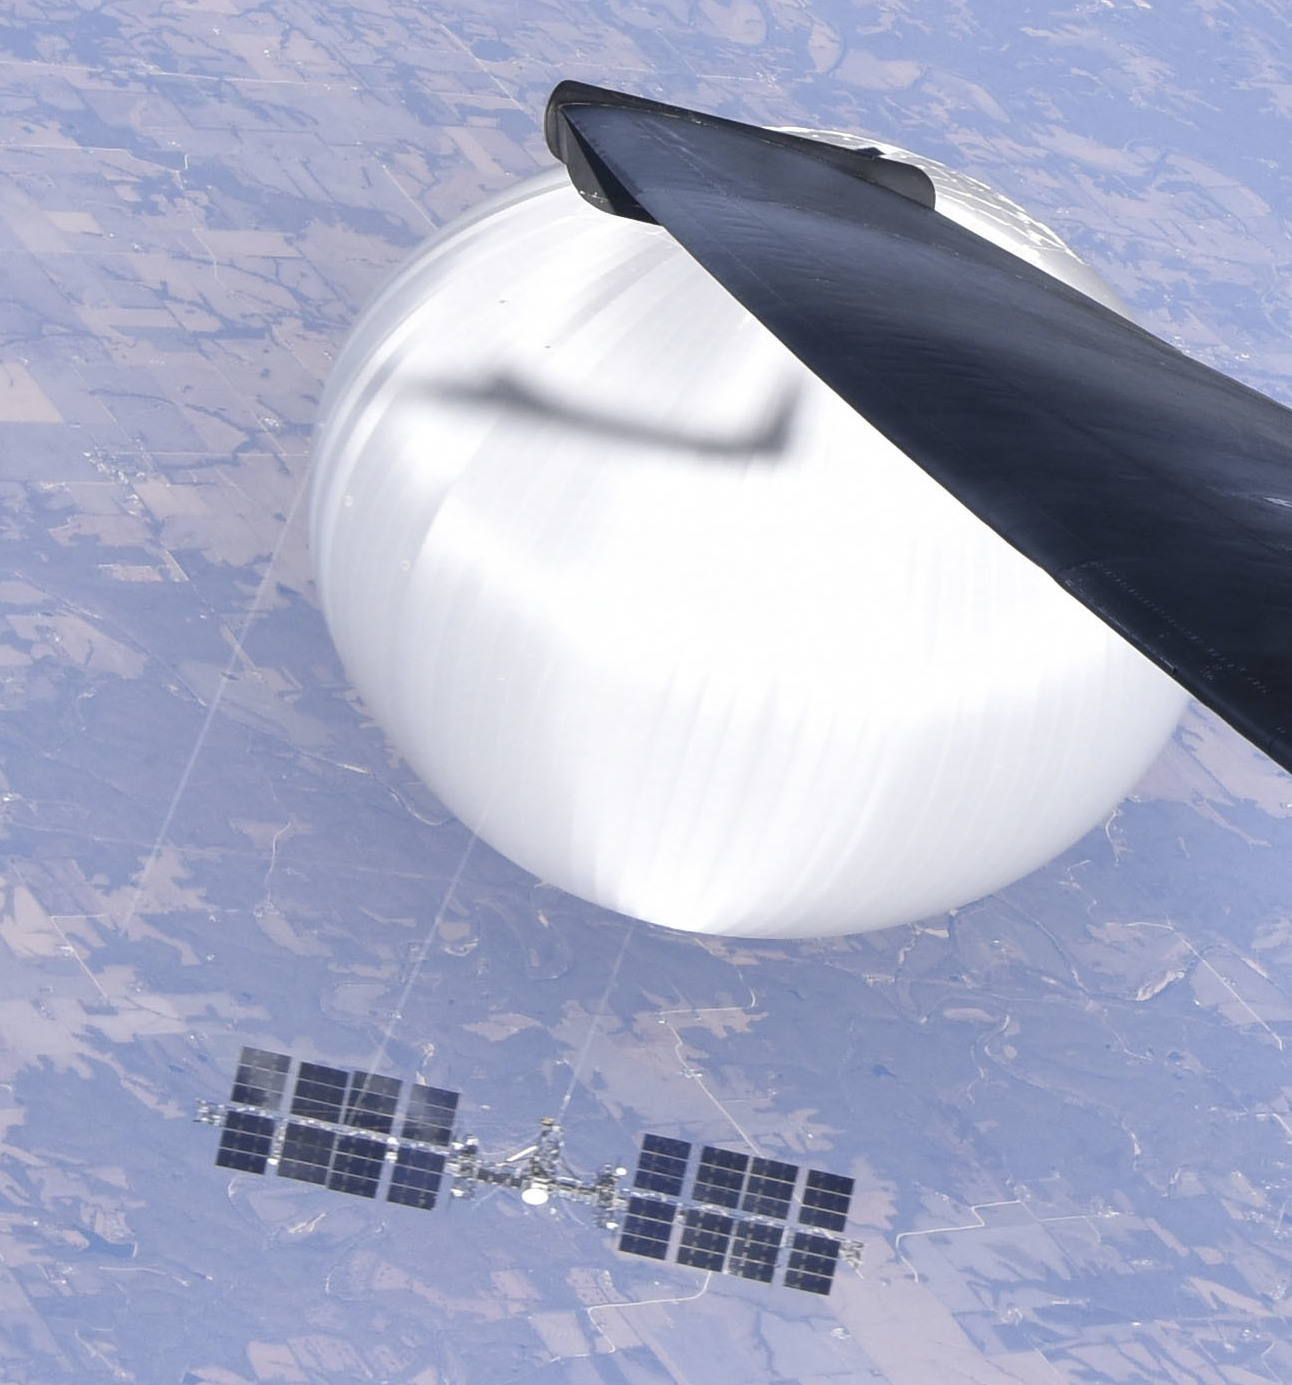
\includegraphics[width=70mm]{figures/U-2_Pilot_over_Central_Continental_United_States_(7644960)_(cropped).jpg}
  \caption{Chinese surveillance balloon over the Central United States as photographed from a U.S. Air Force U-2 on February 3. High altitude balloons have potential for aerial signals intelligence due to their low radar cross section and the wide area of coverage arising from their stratospheric cruising altitude \cite{tomme2005paradigm}.}
  \label{fig-chinese-balloon}
\end{figure}

High altitude balloons are also an interesting platform type when considering their applicability for signals intelligence. These systems are mainly interesting due to their low radar cross section and the wide area of coverage enabled by their relatively high stratospheric cruising altitude \cite{tomme2005paradigm}. Figure \ref{fig-chinese-balloon} shows the Chinese surveillance balloon flting over the Continental United States as photographed from a U.S. Air Force U-2 during an widely reported incident in early 2023.

The goal of the experimental portion of this thesis is to evaluate vulnerability of VSATs to airborne adversaries. Key factors for the evaluation are the ones that define an aircraft's performance: cruising speed and altitude, as well as payload mass, endurance and maneuverability. The latter is especially interesting, as it can greatly vary between platform types. For example, lighter than air crafts, such as high altitude balloons have relatively limited maneuverability, as they rely on athmospheric air currents to carry them around.

\subsection{Communications security}
\subsubsection{Theory of secure communications channels}
Fundamentally, secure communications rely on two core objectives being fulfilled.
The intended receiver should be able to recover the original message without errors, while nobody else should be able to acquire any of the contained information.
As is customary in cryptography, the transmitter is often referred to as Alice, the receiver as Bob and the eavesdropper as Eve.
\cite{bloch2011physical} 
This core principle of secure communications was formalised by Shannon \cite{shannon1949communication} in his seminal 1949 paper through the notion of perfect secrecy achieved through a one-time pad.
Shannon's secrecy system assumes that both the intended recipient and the eavesdropper acquire the encoded codeword without any degradation, i.e. the communication channel is error-free.
This theoretical assumption applies very rarely to real world systems, where some noise is almost always present.
\cite{bloch2011physical}

Wyner \cite{wyner1975thewiretap} expanded on Shannon's original system by exploring the role of noise in the context of secure communications through the channel model called \textit{degraded wiretap channel} (DWTC).
The model assumes a situation where the sender (Alice) attempts to communicate with the legitimate recipient (Bob) over a noisy channel.
Simultaneously an eavesdropper (Eve) observes a degraded version of the signal received by the legitimate recipient.
\cite{barros2006secrecy}
Wyner's wiretap channel introduced many mathematical tools for modelling information-theoretic security without the added complexity of fully general channel models.
One of these important concepts is the secrecy capacity of the channel, which describes the greatest amount of information that can be confidentially communicated between the legitimate transmitter and receiver from the information-theoretic secrecy perspective.
\cite{bloch2011physical}

Csiszár and Körner \cite{csiszar1978broadcast} developed a more general approach that they termed the \textit{broadcast model with confidential messages}.

These seminal works form the foundation for physical layer security research.

Experimental portion of the thesis will examine security of 

% TODO: Sidosteisuutta muuhun tekstiin, physical security, cia triad.

\subsubsection{Signals intelligence: ELINT, COMINT and FISINT}
U.S. Department of Defense (DoD) terminology serves as the foundational framework for discussions on diverse facets within the realm of signals intelligence.
Essential principles of doctrine, guiding the coordinated and integrated application of U.S. military force, are detailed in Joint Publications (JPs) published by the U.S. Joint Chiefs of Staff.
These publications establish foundational doctrinal framework, ensuring standardized procedures for planning, executing, and evaluating military operations, playing an integral role in facilitating a common understanding and synchronized efforts across various branches of the U.S. military.

Within this landscape, intelligence practices are covered in the JP 2-0 Intelligence Series.
JP 2-0 \cite{jp2-0}, titled \textit{Joint Intelligence} and serving as the keystone document of the series, provides the doctrinal foundation and fundamental principles guiding joint and national intelligence products, services, and assessments in support of joint operations.
In JP 2-0, the domain of signals intelligence (SIGINT) is categorized into three distinct subdomains. Communications Intelligence (COMINT) involves gathering intelligence from intercepted foreign communications via radio, wire, or electromagnetic means, extending to encoded imagery.
Electronic Intelligence (ELINT) focuses on non-communications emitters like radar, with operational electronic intelligence emphasizing operationally relevant information and technical electronic intelligence delving into technical aspects of the target systems.
Lastly, Foreign Instrumentation Signals Intelligence (FISINT) analyzes data from foreign equipment and control systems, offering insights into telemetry, electronic interrogators, and command systems, providing a comprehensive understanding of foreign technological capabilities.
In other SIGINT methodologies \cite{kosola2013digitaalinen}, FISINT is often grouped together into ELINT when its definition is taken in the broader non-communications sense.

Signals intelligence (SIGINT) is intelligence gathering through the exploitation of communication systems and noncommunications emitters.
Based on the nature of the target system, the discipline of SIGINT can be further subdivided into the sub-disciplines of communications intelligence (COMINT) and electronic intelligence (ELINT) \cite{national2015bulk} [JP 1-02, JP 2-0 (2013), JP 3-85].

Considering satellite communication systems, the two disciplines of signals intelligence provide a wide range of tools for intelligence gathering at different levels of abstraction.
On the most resource-intense end, we have the interception and extraction of user traffic, the defined scope of COMINT.
However, less sophisticated methods, such as signal detection and fingerprinting, direction finding (DF) and radiopositiong may still yield valuable insights into the nature of the utilized systems, the user organisations, use patterns.
As no 

Interception of user traffic in satellite networks falls under the discipline COMINT. On  based on methods such as time of 

\subsubsection{Electronic warfare: attack, protection and support}

\begin{figure}[h]
  \centering
  \begin{tikzpicture}[
 declare function={
   boxunit=1cm;
   boxsep=0.2cm;
   bigboxW=boxunit*4 + 3*boxsep;
   midboxW=boxunit*2 + boxsep;
 },
 box/.style={draw,minimum width=#1},
 box/.default={boxunit}
]

\node [box=bigboxW,name=1] {1};

\begin{scope}[
  start chain=r1,
  node distance=boxsep-\pgflinewidth,
  every node/.style={box=boxunit, on chain}
]

\node [below=boxsep-\pgflinewidth of 1.south west,anchor=north west] {2};
\node {3};
\node {4};
\node {5};
\end{scope}

\begin{scope}[
  start chain=r2,
  node distance=boxsep-\pgflinewidth,
  every node/.style={box=boxunit, on chain}
]

\node [below=boxsep of r1-1.south west,anchor=north west] {6};
\node {7};
\node {8};
\node {9};
\end{scope}

\begin{scope}[
  start chain=c1 going below,
  node distance=boxsep-\pgflinewidth,
  every node/.style={box=midboxW, on chain}
]

\node [below=boxsep of r2-1.south west,anchor=north west] {10};
\node {12};
\node {14};
\end{scope}

\begin{scope}[
  start chain=c2 going below,
  node distance=boxsep-\pgflinewidth,
  every node/.style={box=midboxW, on chain}
]

\node [below=boxsep of r2-3.south west,anchor=north west] {11};
\node {13};
\node {15};
\end{scope}

\node [inner sep=boxsep,fit=(1)(c2-3),draw] {};

\end{tikzpicture}
  \caption{Electronic warfare taxonomy based on \cite{kosola2013digitaalinen}.}
  \label{fig-electronic-warfare}
\end{figure}

EW involves military actions leveraging Electromagnetic (EM) and Directed Energy (DE) to either control the Electromagnetic Spectrum (EMS) or to launch attacks against the enemy. This multifaceted domain comprises three distinct divisions: Electronic Attack (EA), Electromagnetic Support (ES), and Electromagnetic Protection (EP).

ES involves actions to search for, intercept, identify, and locate or localize sources of intentional and unintentional radiated electromagnetic energy. It serves immediate threat recognition, aids in targeting, contributes to planning, and supports the conduct of future operations on a tactical level. Despite the similarities, ES is a separate discipline from SIGINT. The distinction between the two is delineated by purpose, scope, and context. While ES is focused on immediate operational needs, it shares commonalities with SIGINT, with both potentially using the same assets to simultaneously collect information meeting operational and intelligence requirements.
To quote JP3-85 \cite{jp3-85}, "it can be said that information collected from the EMS has “two lives.” The first is as ES, unprocessed information used by operational forces to develop and maintain SA for an operationally defined period of time. The second is as SIGINT, retained and processed under appropriate intelligence authorities in response to specified intelligence requirements." % TODO: Example methods include eavesdropping, direction finding and z.

Electronic Attack (EA) constitutes another key facet of EW, deploying electromagnetic energy, directed energy, or antiradiation weapons to attack enemy personnel, facilities, or equipment. The intent is to degrade, neutralize, or destroy the combat capability of the adversary. This division, also known as EA, is considered a form of fires within the military context, illustrating its role in directly influencing and diminishing enemy combat effectiveness.

The third division, Electromagnetic Protection (EP), encompasses actions taken to shield personnel, facilities, and equipment from the detrimental effects of friendly or enemy use of the electromagnetic spectrum. EP is essential for maintaining the integrity and functionality of friendly combat capability in the face of electromagnetic threats.

On the practical side, ES is often intelligence gathering and dissemination while EA is direct actions like jamming. EP not concerned with affecting a target system or gaining information, but rather protecting systems from external elec threats.

\subsubsection{TRANSEC and physical layer constraints}
%TODO: Transec 

\subsubsection{Signal detection}
%TODO: Digitaistelukentästä jotain? Siuppaus, ilmaisu etc. ketju? Linkkibudjetti lähtökohtana, spread spectrum?

\subsubsection{Direction finding and radiopositioning}
Geolocating fixed VSAT terminals implemented as phased arrays, different direction finding techniques can be assessed for their suitability based on several factors.
Some of the modern techniques include:

Angle of Arrival (AoA): AoA techniques can be suitable for geolocating VSAT terminals.
By measuring the angles from which the signals arrive at the aircraft's direction finding array, the azimuth and elevation of the terminals can be estimated.
AoA techniques like beamforming, MUSIC, or ESPRIT can be effective in estimating the angles of arrival, especially if the phased array terminals have discernible sidelobes or beam characteristics.

Time Difference of Arrival (TDOA): TDOA relies on measuring the time delays between signals received at multiple spatially separated sensors.

Frequency Difference of Arrival (FDOA): FDOA relies on measuring the frequency differences of signals arriving at different sensors or antennas.
FDOA techniques may provide useful information if the signals have specific frequency characteristics or modulation patterns that can be exploited.

Beamforming: Since phased array VSATs employ beamforming, the listeners direction finding array can analyze the received signals' phase and amplitude information to estimate the direction of arrival.

Additionally, multiple techinques can be combined into a hybrid approach if the complexity and capabilities of the direction finding array permit.
For example, combining AoA and beamforming techniques can enhance the accuracy and robustness of geolocation estimates, especially if the phased array terminals exhibit unique radiation patterns or have challenging sidelobe characteristics.

\clearpage

\subsection{Critical communications}
\subsubsection{Narrowband-to-broadband evolution}
Critical communications are entering a major paradigm shift. Thus far, national authorities have relied globally on dedicated, purpose-built narrowband technologies such as TETRA, Tetrapol and P25 in their operational communications. Broadband standardisation initiated by The Critical Communications Association (TCCA) Critical Communications Broadband Group (CCBG) in 2012 and developed in a working group of 3GPP’s Technical Specification Group since 2015 have adapted the commercial 4G/5G standards to the strict requirements of critical communications. Roll-out of systems built around these standards is currently ongoing in many countries, for example through migration projects such as VIRVE2 in Finland, RRF in France or ESN in the United Kingdom.

The evolution is not limited to just wireless communication technology. In the public safety context, the shift to the more versatile broadband ecosystem enables transitioning from the current voice-only operating model to a more diverse one with voice, video and data capabilities. The higher versatility necessitates reliable access to magnitudes greater bandwidth for them to function. In narrowband networks, building coverage was often the main factor to be considered. On the other hand, ensuring adequate capacity alongside coverage requires additional consideration in broadband networks \cite{saynevirta2021satellite}.

The broadband transition also means a shift from custom technology solutions to more mainstream ones. Critical communications segment places strict requirements on availability, reliability, security, and coverage. For example, the coverage requirement for a national critical communications network can be close to 100 percent of the geographic coverage, while commercial networks are built based on a business case primarily driven by population density. In general, this leads to coverage figures far from 100 percent \cite{saynevirta2021satellite}.

\subsubsection{Use cases and scenarios}
% FIGURE CRITICAL COMMS ARKKITEHTUURI AGNET OVER SATCOM.

Critical communications service operators see satellite systems as a complementary coverage and capacity solution, where the main use cases can be characterised through how long lasting and planned the events requiring response are.
On a high level, the coverage and capacity needs can be either permanent, planned temporary or unplanned temporary in nature.
Prevalent geographic conditions and duration of active use tend to be the determining factors that decide which of the cases is the most applicable in each situation.

Permanent applications tend to be the most obivious when it comes to the typical locations. They encompass the traditionally difficult-to-serve regions.
For example, sparcely populated rural areas and maritime settings have been typically rather poorly served by mobile network operators due to their limited commercial potential.
On the other hand, the temporary use cases tend to be more varied in terms of the potential types of locations. While coverage augmentation is typically still needed only in underserved locations, capacity needs may arise in areas with normally sufficient terrestrial coverage.
For example, large events are a typical example of temporary use cases that can be planned for in advance. These include mass events like sports and concerts and political events like state visits and summits \cite{erve2018trump, tcca2021airbus, airbus2023bahrain}.
Unplanned events can be both man-made or acts of nature and can range from localised to widespread in affected area. For example, natural disasters, like earthquakes, floods, or forest fires, can lead to widespread infrastructure damage, while man-made disasters like airplane crashes or multiple vehicle collisions are usually more limited in terms of the affected area \cite{firstnet2021wildfire, firstnet2021nashville}.

Another differenciating factor of the above mentioned events is their forecastability and typical duration. Both planned and unplanned events can last from days to months, with the duration having different implications for the choice of the best suited technological solution. Satellite connectivity may even be needed permanently when it comes to backhaul applications in very remote locations to where building terrestrial connectivity might be simply unfeasible.
The cut to planned and unplanned events is also not really black-and-white, but these notions exist on a spectrum of different tones of grey. For example, natural disasters such as earthquakes might cause unplanned damage that requires immediate response. On the other hand, some weather events, such as hurricanes and forest fires may be forecasted to differing extents.

All in all, satellite connectivity does not replace the traditional terrestrial networks but complements them. If deployed to their envisioned state, broadband satellite systems may work as a cost-efficient way to serve these regions and events. Thanks to their truly global coverage pattern, while the lower user density in these regions is still within the load carrying capacity of these networks.

\subsubsection{Requirements}

Public Safety users have stringent data security requirements for their communications due to the sensitive nature of these exchanges. Satellite links bring new considerations in the transit of the data through other nations, as the networks are inherently global in nature. In the commercial operating model the constellations downlink data at sites that are most convenient for their operation, which means that the data will often transit through other sovereign countries before arriving at its final destination. Over-the-air transmission of data presents also questions on the jamming resilience of the satellite links.

This poses challenges during situations where a nation is under an external threat, be it a military conflict or an act of a rogue organisation, as sensitive operational information needs to remain only in the hands of its intended users. In addition to these general architectural considerations, the technical solutions themselves should be verifiable on the national or at least at the EU level for both the hardware and software.

Preparedness is a key aspect in the operating model of public safety organisations. It covers the actions required for ensuring the smooth execution of tasks central to the overall safety of a nation in large emergency situations and societal disruptions. Preparedness actions include contingency planning, continuity management, advance preparations, training of operatives and readiness exercises. The concept revolves around the goal of anticipating threats rather than having to react to them [12].

In the case of public safety communications, this leads to high requirements for availability even in a state of emergency. Similarly to more traditional terrestrial solutions, the requirements apply also to the emerging satellite links, which will most likely serve as a back-up solution in the case of larger scale failures of other options.

Satellite links are likely the best suited to natural disasters and major accidents but open questions remain related to human-made threat situations, like terrorist attacks and military conflicts, where external actors may deliberately interfere with the communications links. This raises questions on the political regimes where these current and future constellations are owned and operated. Nationally controlled satellite communications solutions would be the most optimal but are unfeasible for most of the World’s nations to implement. This is due to the immense capital requirements, especially when considering LEO options, which require at minimum hundreds and often thousands of satellites.

These budgetary requirements lead to a situation where most nations need to rely on satellite services that are provided by operators from foreign countries. As discussed later, many of the emerging new operators are either US or UK based, while the EU has also been considering entering the constellation sector with its own alternative. In the EU member state context the latter is probably the most attractive option, especially from the point of critical communications. Control over the constellation and its ground segment will be as close to the national level as is feasible with the capital intensive satellite systems. US and UK based solutions might be also in this sense allowable but are likely to require significant legislative work when used by governmental public safety users.

Straightforward usability of the systems is highly critical from the perspective of public safety users based on the interviews with Finnish Public Safety actors. The success rate in emergency situations depends heavily on the timeliness of the response, which means that the communication systems used in field activities need to be available on a standby-basis. Thus, the future satellite link would need to be highly integrated with the existing communications infrastructure for it to be effective, so that it can be used when necessary.

Considering these usability requirements, an ideal user terminal would be a handset with integrated satellite communication capabilities, but this is not feasible with the current satellite terminal sizes. The more feasible alternative in the near-term would be the integration of the terminal to the vehicles used by the authorities in daily activities.

In addition to conveniently sized and well integrated user terminals, satellite services should be agnostic to the applications that are run through the link they provide. Currently used applications include PTT, data and video, while in future the systems should be able to accommodate more complex applications, like the verified positioning services provided by the Galileo Public Regulated Service (PRS). This may though require special arrangements in timing critical applications, as satellite systems have longer end-to-end delay times compared to terrestrial systems.

Cost considerations are another important point of discussion as they have been a limiting factor for the adoption of the existing satellite services. The new constellations need to achieve significantly lower per user costs for the solutions to gain widespread adoption. The public safety sector is a niche market from the point of view of the constellation operators, which is especially the case for smaller countries like Finland. Volume based pricing models are a possible way of achieving cost advantages but are likely to require the tendering processes to include multiple possible user groups. One straightforward model for providing satellite access to the user organisations could be to include it to the services provided by a national critical communications operator (e.g. Erillisverkot in Finland).

For the solutions to become widely used, their monthly cost should be tens of euros for an individual user terminal. If implemented as a vehicular solution, these kinds of monthly costs would lead to a country wide cost in millions of euros.

\subsubsection{Technical considerations}

Implementation-wise, permanent use cases are maybe the most straight forward, as they are can be implemented as a simple FSS backhaul link of an individual base station site. Direct satellite connectivity is also something that may be feasible in these regions long-term, but as was discussed in chapter \ref{ch-constellation-characteristics}, its technological maturity remains relatively low. 

Implementation-wise, satellite networks are in the short-to-medium term envisioned to integrate into the terrestrial networks through portable tactical bubbles, where the satellite link serves as a backhaul solution for a local (?100 meters to kilometers?) wireless connectivity bubble. In practice, current equipment form factor and cost supports best a vehicular deployment model. For example the French RRF envisions satellite networks as one backhaul option for its vehicular relay (\textit{relais véhiculaire}), an emergency vehicle with a tactical bubble for local coverage and capacity. On the other hand, integration point for satellite systems in the Finnish VIRVE2 has been envisioned as command vehicles of fire, rescue and police forces \cite{RRF_VIITE,saynevirta2021satellite}.

Long-term, evolution towards direct-to-smartphone type solutions is a potential development path. 3GPP has been working towards integrating satellite connectivity as one of the options in the 5G Non-terrestial networks (NTN), a development item also present on the longer-reaching 6G roadmaps \cite{6G_ROADMAP, 3GPP_NTN_PAPERS}. It is though worth noting, that these solutions remain rather low in terms of their technological maturity. In-orbit demonstrations of the technology have been very limited in number and work has focused more on the theoretical standardisation work %TODO: \cite{AST_TESTIT, LYNK_TESTIT, SPACEX_TESTIT, PAPEREITA}

Heikkilän taulukko

\begin{table}[]
  \centering
  \caption{Essential requirements for tactical bubbles \cite{heikkila2021field}.}
  \begin{tabular}{@{}lll@{}}
  \toprule
  Communication type            & Requirement category  & Identified requirements \\ \midrule
  Generic                       & Availability          & 99\% to 99.999\%        \\
                                & Start-up time         & 0 to few minutes        \\
                                & Configuration efforts & Zero-configuration      \\
  Combined user traffic (avg.)  & Downlink / user       & 50 Mbps                 \\
                                & Uplink / user         & 25 Mbps                 \\
  Push to talk                  & Packet delay          & 75 ms                   \\
  Group video                   & Packet delay          & 100 ms                  \\
  Virtual reality (4K GC video) & Data rate             & 50 to 200 Mbps          \\
                                & Latency               & \textless 16 ms         \\
  Sensor data                   & Sensor amount / cell  & 0 to massive            \\
  Machine remote control (UAV)  & Latency               & 40 ms to 1 s            \\ \bottomrule
  \end{tabular}
  \label{table-mcx-requirements}
\end{table}

% Yarali. Tästä voisi vääntää CIA-kolmion

In this section, we address the important security features of the TETRA network.
Here the scope of coverage spans the authentication, encryption mechanisms, and the key management of TETRA.
It dictates that a secure communication network needs to provide (Stavroulakis, 2007):

    Confidentiality
    Integrity
    Reliability
    Non‐repudiation
    Authentication.

6.7.8.1 Confidentiality

    Only authorized personnel or people should have access to the information being passed along.

6.7.8.2 Integrity

    This refers to the requirement that states that only authorized users need to be able to make any modifications to the information in exchange.

6.7.8.3 Reliability

    This refers to the requirement that the resources and the services are not denied and are available to the authorized users to accomplish various tasks.

6.7.8.4 Non‐repudiation

This requires that the sender cannot deny that he/she sent the message.
6.7.8.5 Authentication

    This refers to the requirement that the sender's identity is verifiable by the recipient.

\clearpage

\section{Research material and methods}

\subsection{Methodology}

\begin{figure}[h]
  \centering
  \usetikzlibrary{trees}

\tikzstyle{bag} = [align=center]

\begin{tikzpicture}[level distance=1.5cm,
    level 1/.style={sibling distance=4cm},
    level 2/.style={sibling distance=8cm},
    level 3/.style={sibling distance=4cm}]
  \node {research}
    child {node [bag] {approaches \\ studying reality}
      child {node [bag] {research stressing \\ what is}
        child {node [bag] {\textbf{conceptual-analytical} \\ \textbf{approaches}}}
        child {node [bag] {approaches for \\ empirical studies}
          child [bag] {node {theory-testing \\ approaches}}
          child [bag] {node {theory-creating \\ approaches}}
        }
      }
      child [bag] {node {research stressing \\ utility of}
        child [bag] {node {innovation-building \\ approaches}}
        child [bag] {node {innovation-evaluation \\ approaches}}
      }
    }
    child {node [bag] {mathematical \\ approaches}};
\end{tikzpicture}
  \caption{Research approach taxonomy of Järvinen \cite{jarvinen2011tutkimustyon, jarvinen2004research}. Conceptual-analytical approach followed in this thesis is highlighted.}
  \label{fig-research-taxonomy}
\end{figure}

Järvinen \cite{jarvinen2011tutkimustyon, jarvinen2004research} offers a comprehensive framework for categorizing research approaches, building upon the foundation laid by March and Smith \cite{march1995design}. This taxonomy constitutes six distinct research approaches: mathematical, conceptual-analytical, theory-testing, theory-creating, innovation-building, and innovation-evaluating. Mathematical approaches primarily engage with abstract concepts detached from the constraints of the real world, while research approaches studying reality fall into two main categories—natural and social science approaches (conceptual-analytical, theory-testing, and theory-creating) and design science approaches (innovation-building and innovation-evaluating). The taxonomy proposed by Järvinen in \cite{jarvinen2011tutkimustyon, jarvinen2004research} is presented in figure \ref{fig-research-taxonomy}.

Within the taxonomy, this thesis falls under the conceptual-analytical research approach, the scope being technology-oriented in nature. This approach relies on logical reasoning and draws extensively from prior research and established theories. Conceptual-analytical approaches within the natural and social sciences do not necessarily rely on empirical data, while theory-testing and theory-creating approaches use data to either validate existing theories or formulate new ones. The primary objective of conceptual-analytical research is to generate new creating theoretical concepts or analysing existing theories.

In practical terms, the modelling approach in this thesis is grounded on theoretical background of RF systems and more specifically concepts related to electronic warfare and signals intelligence. Threat model builds upon theory discussed in \cite{kosola2013digitaalinen} and \cite{wiley2006elint}. Target systems are explored through a parametric study of an analyitical model comprised of multiple submodels that incorporate relevant parameters for aerial signals intelligence platforms and both space and ground segments of a satellite communications system.

\subsection{Data sources}

% TODO: Data sources satellite systems: FCC filings for space segment and user terminals, UT product data sheets, 

% TODO: Datalähteet: ilma-alusket, uas, manned, balloon

\section{Results}

\subsection{Threat model}
The core goal of this thesis is to assess whether the presence of airborne eavesdroppers poses a risk to the uplink communications of emerging NGSO VSAT networks.
The research applies quantitative analysis by building a threat model focusing on a Walker-type LEO megaconstellation, fixed Very Small Aperture Terminals (VSAT) and airborne eavesdroppers.
The threat model is built around a set of four smaller submodels, each examining analytically a relevant dependent variable against a number of independent ones.
The models are first introduced in a deductive manner tying reality to the underlying theoretical concepts.
Individual submodels are then parametrically studied in a range of starting conditions mirroring the relevant characteristics of the platforms under evaluation.
Descriptions for the submodels are given in table \ref{table-sub-model-descriptions} while their independent and dependent variables of the parametric study are introduced in table \ref{table-sub-model-variables}.

The models explore the target system from first principles using geometric and kinematic analysis, as well as link budgets based on an example hardware configuration.
First principles thinking is a powerful problem-solving approach that involves breaking down a problem or a concept into its elemental parts.
In this sense, each submodel helps us understand potential strengths and vulnerability of different satcom systems through an elemental understanding of the underlying physical phenomena. %% TODO: Miksi relevantteja tutkittavia asioita? DONE?

Critical communications users place high expectations on the communications solutions that they utilise.
Satcom solutions have seen previously somewhat limited especially in the public safety sector, while at the same time commercial systems have turned out to be not the most robust when it comes to to fundamental concepts of security, such as confidentiality, integrity and availability.
With the recent drive to integrate satcom into both commercial and critical use cases, it is paramount to understand the underlying factors of the systems.
Physics-driven analysis helps us to evaluate the limits of a systems in a way that allows for sufficient risk mitigations to be engineered. %% TODO: Miten liittyy public safety caseen? DONE?

\begin{table}[h]
  \centering
  \caption{Descriptions for the sub-models.}
  \begin{tabular}{@{}cl@{}}
  \toprule
  \multicolumn{1}{l}{sub-model} & target metric                              \\ \midrule
  1                             & maximum interception range                 \\
  2a                            & beam tracking potential, equatorial orbits \\
  2b                            & beam tracking potential, inclined orbits   \\
  3                             & listening window                           \\
  4                             & jamming link budget                        \\ \bottomrule
  \end{tabular}
  \label{table-sub-model-descriptions}
\end{table}

Submodel 1 examines the maximum interception range of a fixed satellite terminal.
This metric helps us to evaluate the potential maximal area where a single satellite terminal is vulnerable to airborne eavesdroppers.
Airborne platforms may listen to transmissions from great distances, for example flying in an airspace of another country.
Submodels 2 and 3 examine an aircraft's ability to track an UT's RF beam.
VSATs have typically a relatively narrow beam pattern of a few degrees of half power beamwidth.
Relative motion between the beam and an intercepting aircraft is a major consideration when it comes to evaluating the vulnerability of different satellite systems.
Submodel 4 examines the a jammer's ability to interfere with a legitimate UT interfacing with a LEO megaconstellation.
Link budget for an uplink connection from an UT to a satellite is computed.
In the scenario, the jammer competes with the legitimate transmitter in RF signal power received by the satellite.

\begin{table}[h]
  \centering
  \caption{Independent and dependent variables of the sub-models.}
  \begin{tabular}{@{}cll@{}}
  \toprule
  Sub-model &
    Dependent variable &
    Independent variables \\ \midrule
  1 &
    interception range (m) &
    \begin{tabular}[c]{@{}l@{}}minimum elevation angle (deg)\\ eavesdropper’s altitude (m)\end{tabular} \\ \addlinespace[0.5em]
  2a &
    \begin{tabular}[c]{@{}l@{}}velocity of the sub-satellite point,\\ equatorial (m/s)\end{tabular} &
    orbital altitude (m) \\ \addlinespace[0.5em]
  2b &
    \begin{tabular}[c]{@{}l@{}}velocity of the sub-satellite point,\\ inclined (m/s)\end{tabular} &
    \begin{tabular}[c]{@{}l@{}}orbital altitude (m)\\ inclination (deg)\end{tabular} \\ \addlinespace[0.5em]
  3 &
    listening window (s) &
    \begin{tabular}[c]{@{}l@{}}orbital altitude (m)\\ inclination (deg)\\ eavesdropper’s velocity (m/s)\end{tabular} \\ \addlinespace[0.5em]
  4 &
    required jamming power (dBW) &
    target SJNR at RX (dB)
     \\ \bottomrule
  \end{tabular}
  \label{table-sub-model-variables}
\end{table}

\subsection{Submodel 1: Maximum interception range} \label{ch-results-submodel-1-range}
% TODO: Scenario description: häritsijän sijainti, muuttujat -> orientoiva
In order to eavesdrop a target transmitter, an eavesdropper need to be able to intercept sufficiently strong uplink signal. 
Being firmly out of range of an earth station, in other words inside a white zone, is the most fundamental limit to an eavesdropper's ability to eavesdrop. 
This can be thought as  arise where eavesdropping is either simply impossible or a very tough uphill battle:

\begin{enumerate}
  \item The VSAT earth station falls behind the radio horizon of the eavesdropper.
  \item The eavesdropper falls outside the main lobe of the VSAT earth station.
\end{enumerate}

As presented in appendix \ref{appendix-constellation-comparison}, broadband VSAT systems both existing and under development tend to operate in the Ku and Ka bands (12--18 and 26.5--40 GHz respectively), with the former being the more commonly used in user links between the orbiting satellite and user terminal and vice-versa, although some systems, such as Amazon's Project Kuiper deviate from this "rule". % TODO: Parempi termi
In terms frequencies, both bands fall under super high (SHF, 3-30 GHz) to extremely high frequencies (EHF, 30-300 GHz), where the principal propagation mode is line-of-sight propagation.
In this mode, the radio horizon of a transmitter can be derived from the Pythagorean theorem, assuming a perfectly spherical planetary body.

Going into the geometry of the problem, line-of-sight distance $d$ and radius of the body $R$ form the legs of a right triangle, while the transmitter's distance from the centre of the body $(R+h)$ is the hypotenuse \cite{seybold2005introduction}.
The relationship between the quantities is visualised in figure \ref{fig-interception-range-vacuum}.

% TODO: SELITÄ MIKSI VOIDAAN APROKSIMOIDA TOISESSA VIRKKEESSÄ

\begin{equation*}
  d^2=(R+h)^{2}-R^2= 2R \cdot h + h^2 \\
\end{equation*}

In case of the Earth, the height of both surface-bound and airborne transmitters $h$ is rather insignificant compared to the radius of the body $R$. Thus, we can simplify the line-of-sight equation to

\begin{equation} \label{eq-radio-horizon-vac}
  d \approx \sqrt{2R \cdot h}
\end{equation}

It is worth noting that equation (\ref{eq-radio-horizon-vac}) applies only in vacuum.
Vertical pressure variation of an athmosphere refracts passing electromagnetic waves. In practice, the waves deviate from a straight line down towards the surface. This deviation can be accounted for by applying a factor $k$ to equation (\ref{eq-radio-horizon-vac}). In case of the Earth, an effective radius of $4/3$ is usually applied \cite{seybold2005introduction}.

\begin{equation} \label{eq-radio-horizon-ath}
  d \approx \sqrt{2 k \cdot R \cdot h}
\end{equation}

Radio horizon allows us to examine situations where the transmitting antenna is either isotropic or pointed deliberately in the direction of the horizon.
This is not always the case with highly directional VSAT terminals, thus requiring additional factors being taken into account.
Here, one of the most important parameters is the minimum elevation angle of the satellite system in question.
Similar to radio horizon, maximum VSAT interception range can be examined through a trigonometric approximation model.

As discussed regarding the characteristics of the terminals, typical minimum elevation angles range from 20 to 55 degrees in the recent broadband megaconstellations in LEO.
As the operational altitude of the eavesdropper is known, theoretical maximum interception range can be computed for a range of the minimum elevation angles.
The measurands form an orthogonal triangle with the minimum elevation as the acute angle opposite to the height of the triangle.
The operational altitude of the eavesdropper is the height of the triangle, while the base is formed by the theoretical interception range of the system.
Lastly, the hypotenuse is the line-of-sight (LOS) distance between the VSAT site and the airborne eavesdropper.

Trigonometric tangent function of the interception range triangle is

\begin{equation} \label{eq-range-1}
  \tan(e_{Alice}) = \frac{h_{Eve}}{d_{Eve}}
\end{equation}

\noindent
where $e_{Alice}$ is the minimum elevation angle of the user terminal, $h_{Eve}$ is the operational altitude of the intercepting airborne platform and $d_{Eve}$ is its distance from Alice on the ground, in essence the interception range.
Rearranging (\ref{eq-range-1}) for $d_{Eve}$ gives

\begin{align} \label{eq-range-2}
  d_{Eve} = \frac{h_{Eve}}{\tan(e_{Alice})}
\end{align}

\begin{figure}[h]
  \centering
  % This file was created by matlab2tikz.
%
%The latest updates can be retrieved from
%  http://www.mathworks.com/matlabcentral/fileexchange/22022-matlab2tikz-matlab2tikz
%where you can also make suggestions and rate matlab2tikz.
%
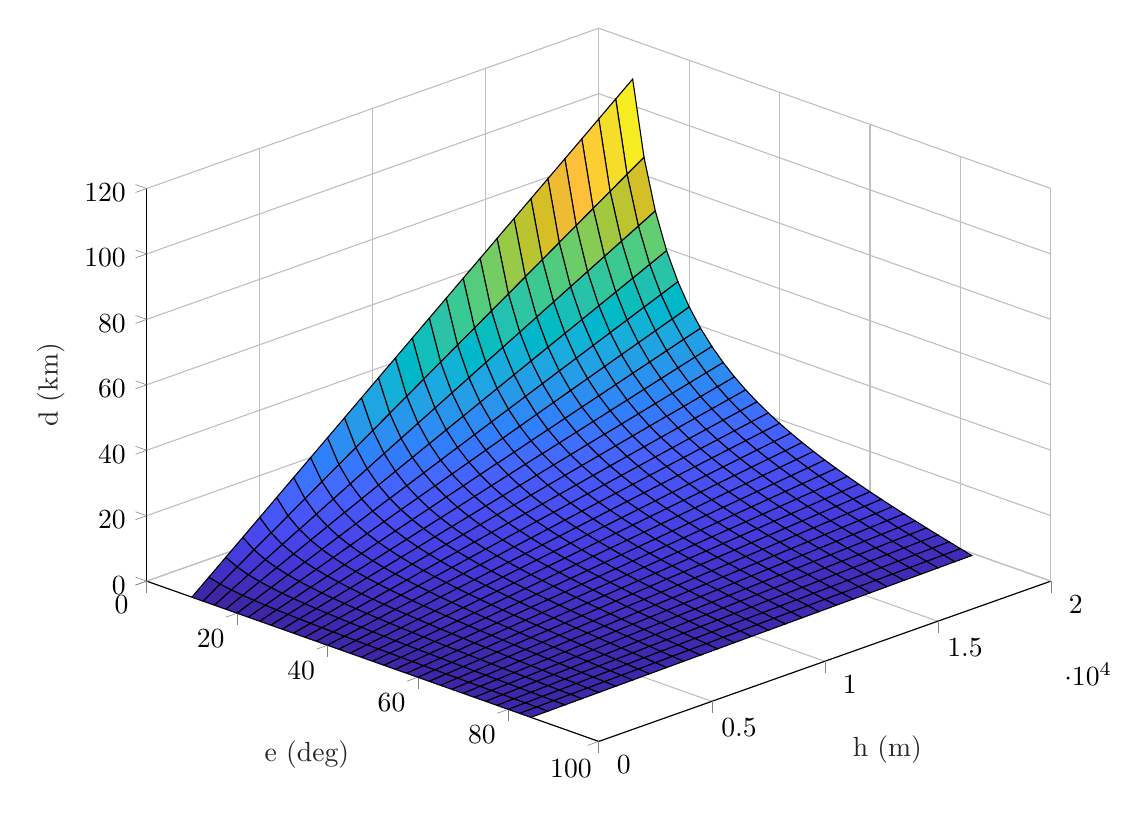
\begin{tikzpicture}

\begin{axis}[%
width=4.521in,
height=3.566in,
at={(0.758in,0.481in)},
scale only axis,
xmin=0,
xmax=100,
tick align=outside,
xlabel style={font=\color{white!15!black}},
xlabel={e (deg)},
ymin=0,
ymax=20000,
ylabel style={font=\color{white!15!black}},
ylabel={h (m)},
zmin=0,
zmax=120,
zlabel style={font=\color{white!15!black}},
zlabel={d (km)},
view={45}{30},
axis background/.style={fill=white},
axis x line*=bottom,
axis y line*=left,
axis z line*=left,
xmajorgrids,
ymajorgrids,
zmajorgrids
]

\addplot3[%
surf,
shader=flat corner, draw=black, z buffer=sort, colormap={mymap}{[1pt] rgb(0pt)=(0.2422,0.1504,0.6603); rgb(1pt)=(0.2444,0.1534,0.6728); rgb(2pt)=(0.2464,0.1569,0.6847); rgb(3pt)=(0.2484,0.1607,0.6961); rgb(4pt)=(0.2503,0.1648,0.7071); rgb(5pt)=(0.2522,0.1689,0.7179); rgb(6pt)=(0.254,0.1732,0.7286); rgb(7pt)=(0.2558,0.1773,0.7393); rgb(8pt)=(0.2576,0.1814,0.7501); rgb(9pt)=(0.2594,0.1854,0.761); rgb(11pt)=(0.2628,0.1932,0.7828); rgb(12pt)=(0.2645,0.1972,0.7937); rgb(13pt)=(0.2661,0.2011,0.8043); rgb(14pt)=(0.2676,0.2052,0.8148); rgb(15pt)=(0.2691,0.2094,0.8249); rgb(16pt)=(0.2704,0.2138,0.8346); rgb(17pt)=(0.2717,0.2184,0.8439); rgb(18pt)=(0.2729,0.2231,0.8528); rgb(19pt)=(0.274,0.228,0.8612); rgb(20pt)=(0.2749,0.233,0.8692); rgb(21pt)=(0.2758,0.2382,0.8767); rgb(22pt)=(0.2766,0.2435,0.884); rgb(23pt)=(0.2774,0.2489,0.8908); rgb(24pt)=(0.2781,0.2543,0.8973); rgb(25pt)=(0.2788,0.2598,0.9035); rgb(26pt)=(0.2794,0.2653,0.9094); rgb(27pt)=(0.2798,0.2708,0.915); rgb(28pt)=(0.2802,0.2764,0.9204); rgb(29pt)=(0.2806,0.2819,0.9255); rgb(30pt)=(0.2809,0.2875,0.9305); rgb(31pt)=(0.2811,0.293,0.9352); rgb(32pt)=(0.2813,0.2985,0.9397); rgb(33pt)=(0.2814,0.304,0.9441); rgb(34pt)=(0.2814,0.3095,0.9483); rgb(35pt)=(0.2813,0.315,0.9524); rgb(36pt)=(0.2811,0.3204,0.9563); rgb(37pt)=(0.2809,0.3259,0.96); rgb(38pt)=(0.2807,0.3313,0.9636); rgb(39pt)=(0.2803,0.3367,0.967); rgb(40pt)=(0.2798,0.3421,0.9702); rgb(41pt)=(0.2791,0.3475,0.9733); rgb(42pt)=(0.2784,0.3529,0.9763); rgb(43pt)=(0.2776,0.3583,0.9791); rgb(44pt)=(0.2766,0.3638,0.9817); rgb(45pt)=(0.2754,0.3693,0.984); rgb(46pt)=(0.2741,0.3748,0.9862); rgb(47pt)=(0.2726,0.3804,0.9881); rgb(48pt)=(0.271,0.386,0.9898); rgb(49pt)=(0.2691,0.3916,0.9912); rgb(50pt)=(0.267,0.3973,0.9924); rgb(51pt)=(0.2647,0.403,0.9935); rgb(52pt)=(0.2621,0.4088,0.9946); rgb(53pt)=(0.2591,0.4145,0.9955); rgb(54pt)=(0.2556,0.4203,0.9965); rgb(55pt)=(0.2517,0.4261,0.9974); rgb(56pt)=(0.2473,0.4319,0.9983); rgb(57pt)=(0.2424,0.4378,0.9991); rgb(58pt)=(0.2369,0.4437,0.9996); rgb(59pt)=(0.2311,0.4497,0.9995); rgb(60pt)=(0.225,0.4559,0.9985); rgb(61pt)=(0.2189,0.462,0.9968); rgb(62pt)=(0.2128,0.4682,0.9948); rgb(63pt)=(0.2066,0.4743,0.9926); rgb(64pt)=(0.2006,0.4803,0.9906); rgb(65pt)=(0.195,0.4861,0.9887); rgb(66pt)=(0.1903,0.4919,0.9867); rgb(67pt)=(0.1869,0.4975,0.9844); rgb(68pt)=(0.1847,0.503,0.9819); rgb(69pt)=(0.1831,0.5084,0.9793); rgb(70pt)=(0.1818,0.5138,0.9766); rgb(71pt)=(0.1806,0.5191,0.9738); rgb(72pt)=(0.1795,0.5244,0.9709); rgb(73pt)=(0.1785,0.5296,0.9677); rgb(74pt)=(0.1778,0.5349,0.9641); rgb(75pt)=(0.1773,0.5401,0.9602); rgb(76pt)=(0.1768,0.5452,0.956); rgb(77pt)=(0.1764,0.5504,0.9516); rgb(78pt)=(0.1755,0.5554,0.9473); rgb(79pt)=(0.174,0.5605,0.9432); rgb(80pt)=(0.1716,0.5655,0.9393); rgb(81pt)=(0.1686,0.5705,0.9357); rgb(82pt)=(0.1649,0.5755,0.9323); rgb(83pt)=(0.161,0.5805,0.9289); rgb(84pt)=(0.1573,0.5854,0.9254); rgb(85pt)=(0.154,0.5902,0.9218); rgb(86pt)=(0.1513,0.595,0.9182); rgb(87pt)=(0.1492,0.5997,0.9147); rgb(88pt)=(0.1475,0.6043,0.9113); rgb(89pt)=(0.1461,0.6089,0.908); rgb(90pt)=(0.1446,0.6135,0.905); rgb(91pt)=(0.1429,0.618,0.9022); rgb(92pt)=(0.1408,0.6226,0.8998); rgb(93pt)=(0.1383,0.6272,0.8975); rgb(94pt)=(0.1354,0.6317,0.8953); rgb(95pt)=(0.1321,0.6363,0.8932); rgb(96pt)=(0.1288,0.6408,0.891); rgb(97pt)=(0.1253,0.6453,0.8887); rgb(98pt)=(0.1219,0.6497,0.8862); rgb(99pt)=(0.1185,0.6541,0.8834); rgb(100pt)=(0.1152,0.6584,0.8804); rgb(101pt)=(0.1119,0.6627,0.877); rgb(102pt)=(0.1085,0.6669,0.8734); rgb(103pt)=(0.1048,0.671,0.8695); rgb(104pt)=(0.1009,0.675,0.8653); rgb(105pt)=(0.0964,0.6789,0.8609); rgb(106pt)=(0.0914,0.6828,0.8562); rgb(107pt)=(0.0855,0.6865,0.8513); rgb(108pt)=(0.0789,0.6902,0.8462); rgb(109pt)=(0.0713,0.6938,0.8409); rgb(110pt)=(0.0628,0.6972,0.8355); rgb(111pt)=(0.0535,0.7006,0.8299); rgb(112pt)=(0.0433,0.7039,0.8242); rgb(113pt)=(0.0328,0.7071,0.8183); rgb(114pt)=(0.0234,0.7103,0.8124); rgb(115pt)=(0.0155,0.7133,0.8064); rgb(116pt)=(0.0091,0.7163,0.8003); rgb(117pt)=(0.0046,0.7192,0.7941); rgb(118pt)=(0.0019,0.722,0.7878); rgb(119pt)=(0.0009,0.7248,0.7815); rgb(120pt)=(0.0018,0.7275,0.7752); rgb(121pt)=(0.0046,0.7301,0.7688); rgb(122pt)=(0.0094,0.7327,0.7623); rgb(123pt)=(0.0162,0.7352,0.7558); rgb(124pt)=(0.0253,0.7376,0.7492); rgb(125pt)=(0.0369,0.74,0.7426); rgb(126pt)=(0.0504,0.7423,0.7359); rgb(127pt)=(0.0638,0.7446,0.7292); rgb(128pt)=(0.077,0.7468,0.7224); rgb(129pt)=(0.0899,0.7489,0.7156); rgb(130pt)=(0.1023,0.751,0.7088); rgb(131pt)=(0.1141,0.7531,0.7019); rgb(132pt)=(0.1252,0.7552,0.695); rgb(133pt)=(0.1354,0.7572,0.6881); rgb(134pt)=(0.1448,0.7593,0.6812); rgb(135pt)=(0.1532,0.7614,0.6741); rgb(136pt)=(0.1609,0.7635,0.6671); rgb(137pt)=(0.1678,0.7656,0.6599); rgb(138pt)=(0.1741,0.7678,0.6527); rgb(139pt)=(0.1799,0.7699,0.6454); rgb(140pt)=(0.1853,0.7721,0.6379); rgb(141pt)=(0.1905,0.7743,0.6303); rgb(142pt)=(0.1954,0.7765,0.6225); rgb(143pt)=(0.2003,0.7787,0.6146); rgb(144pt)=(0.2061,0.7808,0.6065); rgb(145pt)=(0.2118,0.7828,0.5983); rgb(146pt)=(0.2178,0.7849,0.5899); rgb(147pt)=(0.2244,0.7869,0.5813); rgb(148pt)=(0.2318,0.7887,0.5725); rgb(149pt)=(0.2401,0.7905,0.5636); rgb(150pt)=(0.2491,0.7922,0.5546); rgb(151pt)=(0.2589,0.7937,0.5454); rgb(152pt)=(0.2695,0.7951,0.536); rgb(153pt)=(0.2809,0.7964,0.5266); rgb(154pt)=(0.2929,0.7975,0.517); rgb(155pt)=(0.3052,0.7985,0.5074); rgb(156pt)=(0.3176,0.7994,0.4975); rgb(157pt)=(0.3301,0.8002,0.4876); rgb(158pt)=(0.3424,0.8009,0.4774); rgb(159pt)=(0.3548,0.8016,0.4669); rgb(160pt)=(0.3671,0.8021,0.4563); rgb(161pt)=(0.3795,0.8026,0.4454); rgb(162pt)=(0.3921,0.8029,0.4344); rgb(163pt)=(0.405,0.8031,0.4233); rgb(164pt)=(0.4184,0.803,0.4122); rgb(165pt)=(0.4322,0.8028,0.4013); rgb(166pt)=(0.4463,0.8024,0.3904); rgb(167pt)=(0.4608,0.8018,0.3797); rgb(168pt)=(0.4753,0.8011,0.3691); rgb(169pt)=(0.4899,0.8002,0.3586); rgb(170pt)=(0.5044,0.7993,0.348); rgb(171pt)=(0.5187,0.7982,0.3374); rgb(172pt)=(0.5329,0.797,0.3267); rgb(173pt)=(0.547,0.7957,0.3159); rgb(175pt)=(0.5748,0.7929,0.2941); rgb(176pt)=(0.5886,0.7913,0.2833); rgb(177pt)=(0.6024,0.7896,0.2726); rgb(178pt)=(0.6161,0.7878,0.2622); rgb(179pt)=(0.6297,0.7859,0.2521); rgb(180pt)=(0.6433,0.7839,0.2423); rgb(181pt)=(0.6567,0.7818,0.2329); rgb(182pt)=(0.6701,0.7796,0.2239); rgb(183pt)=(0.6833,0.7773,0.2155); rgb(184pt)=(0.6963,0.775,0.2075); rgb(185pt)=(0.7091,0.7727,0.1998); rgb(186pt)=(0.7218,0.7703,0.1924); rgb(187pt)=(0.7344,0.7679,0.1852); rgb(188pt)=(0.7468,0.7654,0.1782); rgb(189pt)=(0.759,0.7629,0.1717); rgb(190pt)=(0.771,0.7604,0.1658); rgb(191pt)=(0.7829,0.7579,0.1608); rgb(192pt)=(0.7945,0.7554,0.157); rgb(193pt)=(0.806,0.7529,0.1546); rgb(194pt)=(0.8172,0.7505,0.1535); rgb(195pt)=(0.8281,0.7481,0.1536); rgb(196pt)=(0.8389,0.7457,0.1546); rgb(197pt)=(0.8495,0.7435,0.1564); rgb(198pt)=(0.86,0.7413,0.1587); rgb(199pt)=(0.8703,0.7392,0.1615); rgb(200pt)=(0.8804,0.7372,0.165); rgb(201pt)=(0.8903,0.7353,0.1695); rgb(202pt)=(0.9,0.7336,0.1749); rgb(203pt)=(0.9093,0.7321,0.1815); rgb(204pt)=(0.9184,0.7308,0.189); rgb(205pt)=(0.9272,0.7298,0.1973); rgb(206pt)=(0.9357,0.729,0.2061); rgb(207pt)=(0.944,0.7285,0.2151); rgb(208pt)=(0.9523,0.7284,0.2237); rgb(209pt)=(0.9606,0.7285,0.2312); rgb(210pt)=(0.9689,0.7292,0.2373); rgb(211pt)=(0.977,0.7304,0.2418); rgb(212pt)=(0.9842,0.733,0.2446); rgb(213pt)=(0.99,0.7365,0.2429); rgb(214pt)=(0.9946,0.7407,0.2394); rgb(215pt)=(0.9966,0.7458,0.2351); rgb(216pt)=(0.9971,0.7513,0.2309); rgb(217pt)=(0.9972,0.7569,0.2267); rgb(218pt)=(0.9971,0.7626,0.2224); rgb(219pt)=(0.9969,0.7683,0.2181); rgb(220pt)=(0.9966,0.774,0.2138); rgb(221pt)=(0.9962,0.7798,0.2095); rgb(222pt)=(0.9957,0.7856,0.2053); rgb(223pt)=(0.9949,0.7915,0.2012); rgb(224pt)=(0.9938,0.7974,0.1974); rgb(225pt)=(0.9923,0.8034,0.1939); rgb(226pt)=(0.9906,0.8095,0.1906); rgb(227pt)=(0.9885,0.8156,0.1875); rgb(228pt)=(0.9861,0.8218,0.1846); rgb(229pt)=(0.9835,0.828,0.1817); rgb(230pt)=(0.9807,0.8342,0.1787); rgb(231pt)=(0.9778,0.8404,0.1757); rgb(232pt)=(0.9748,0.8467,0.1726); rgb(233pt)=(0.972,0.8529,0.1695); rgb(234pt)=(0.9694,0.8591,0.1665); rgb(235pt)=(0.9671,0.8654,0.1636); rgb(236pt)=(0.9651,0.8716,0.1608); rgb(237pt)=(0.9634,0.8778,0.1582); rgb(238pt)=(0.9619,0.884,0.1557); rgb(239pt)=(0.9608,0.8902,0.1532); rgb(240pt)=(0.9601,0.8963,0.1507); rgb(241pt)=(0.9596,0.9023,0.148); rgb(242pt)=(0.9595,0.9084,0.145); rgb(243pt)=(0.9597,0.9143,0.1418); rgb(244pt)=(0.9601,0.9203,0.1382); rgb(245pt)=(0.9608,0.9262,0.1344); rgb(246pt)=(0.9618,0.932,0.1304); rgb(247pt)=(0.9629,0.9379,0.1261); rgb(248pt)=(0.9642,0.9437,0.1216); rgb(249pt)=(0.9657,0.9494,0.1168); rgb(250pt)=(0.9674,0.9552,0.1116); rgb(251pt)=(0.9692,0.9609,0.1061); rgb(252pt)=(0.9711,0.9667,0.1001); rgb(253pt)=(0.973,0.9724,0.0938); rgb(254pt)=(0.9749,0.9782,0.0872); rgb(255pt)=(0.9769,0.9839,0.0805)}, mesh/rows=27]
table[row sep=crcr, point meta=\thisrow{c}] {%
%
x	y	z	c\\
10	0	0	0\\
12.5	0	0	0\\
15	0	0	0\\
17.5	0	0	0\\
20	0	0	0\\
22.5	0	0	0\\
25	0	0	0\\
27.5	0	0	0\\
30	0	0	0\\
32.5	0	0	0\\
35	0	0	0\\
37.5	0	0	0\\
40	0	0	0\\
42.5	0	0	0\\
45	0	0	0\\
47.5	0	0	0\\
50	0	0	0\\
52.5	0	0	0\\
55	0	0	0\\
57.5	0	0	0\\
60	0	0	0\\
62.5	0	0	0\\
65	0	0	0\\
67.5	0	0	0\\
70	0	0	0\\
72.5	0	0	0\\
75	0	0	0\\
77.5	0	0	0\\
80	0	0	0\\
82.5	0	0	0\\
85	0	0	0\\
10	750	4.25346136471328	4.25346136471328\\
12.5	750	3.38303137774654	3.38303137774654\\
15	750	2.79903810567666	2.79903810567666\\
17.5	750	2.37869610177241	2.37869610177241\\
20	750	2.06060806459097	2.06060806459097\\
22.5	750	1.81066017177982	1.81066017177982\\
25	750	1.60838019038217	1.60838019038217\\
27.5	750	1.44073659522837	1.44073659522837\\
30	750	1.29903810567666	1.29903810567666\\
32.5	750	1.17726418283812	1.17726418283812\\
35	750	1.07111100505659	1.07111100505659\\
37.5	750	0.977419029630904	0.977419029630904\\
40	750	0.893815194445657	0.893815194445657\\
42.5	750	0.818481375801953	0.818481375801953\\
45	750	0.75	0.75\\
47.5	750	0.687248380513068	0.687248380513068\\
50	750	0.62932472338296	0.62932472338296\\
52.5	750	0.57549524098422	0.57549524098422\\
55	750	0.525155653657282	0.525155653657282\\
57.5	750	0.47780269560562	0.47780269560562\\
60	750	0.433012701892219	0.433012701892219\\
62.5	750	0.39042528791381	0.39042528791381\\
65	750	0.349730743616249	0.349730743616249\\
67.5	750	0.310660171779821	0.310660171779821\\
70	750	0.272977675699652	0.272977675699652\\
72.5	750	0.236474091659238	0.236474091659238\\
75	750	0.200961894323342	0.200961894323342\\
77.5	750	0.166270996982205	0.166270996982205\\
80	750	0.132245235531349	0.132245235531349\\
82.5	750	0.0987393731905469	0.0987393731905469\\
85	750	0.065616497644443	0.065616497644443\\
10	1500	8.50692272942656	8.50692272942656\\
12.5	1500	6.76606275549308	6.76606275549308\\
15	1500	5.59807621135332	5.59807621135332\\
17.5	1500	4.75739220354482	4.75739220354482\\
20	1500	4.12121612918193	4.12121612918193\\
22.5	1500	3.62132034355964	3.62132034355964\\
25	1500	3.21676038076434	3.21676038076434\\
27.5	1500	2.88147319045675	2.88147319045675\\
30	1500	2.59807621135332	2.59807621135332\\
32.5	1500	2.35452836567624	2.35452836567624\\
35	1500	2.14222201011317	2.14222201011317\\
37.5	1500	1.95483805926181	1.95483805926181\\
40	1500	1.78763038889131	1.78763038889131\\
42.5	1500	1.63696275160391	1.63696275160391\\
45	1500	1.5	1.5\\
47.5	1500	1.37449676102614	1.37449676102614\\
50	1500	1.25864944676592	1.25864944676592\\
52.5	1500	1.15099048196844	1.15099048196844\\
55	1500	1.05031130731456	1.05031130731456\\
57.5	1500	0.95560539121124	0.95560539121124\\
60	1500	0.866025403784439	0.866025403784439\\
62.5	1500	0.780850575827619	0.780850575827619\\
65	1500	0.699461487232498	0.699461487232498\\
67.5	1500	0.621320343559643	0.621320343559643\\
70	1500	0.545955351399304	0.545955351399304\\
72.5	1500	0.472948183318475	0.472948183318475\\
75	1500	0.401923788646684	0.401923788646684\\
77.5	1500	0.33254199396441	0.33254199396441\\
80	1500	0.264490471062697	0.264490471062697\\
82.5	1500	0.197478746381094	0.197478746381094\\
85	1500	0.131232995288886	0.131232995288886\\
10	2250	12.7603840941398	12.7603840941398\\
12.5	2250	10.1490941332396	10.1490941332396\\
15	2250	8.39711431702997	8.39711431702997\\
17.5	2250	7.13608830531723	7.13608830531723\\
20	2250	6.1818241937729	6.1818241937729\\
22.5	2250	5.43198051533946	5.43198051533946\\
25	2250	4.82514057114651	4.82514057114651\\
27.5	2250	4.32220978568512	4.32220978568512\\
30	2250	3.89711431702997	3.89711431702997\\
32.5	2250	3.53179254851435	3.53179254851435\\
35	2250	3.21333301516976	3.21333301516976\\
37.5	2250	2.93225708889271	2.93225708889271\\
40	2250	2.68144558333697	2.68144558333697\\
42.5	2250	2.45544412740586	2.45544412740586\\
45	2250	2.25	2.25\\
47.5	2250	2.0617451415392	2.0617451415392\\
50	2250	1.88797417014888	1.88797417014888\\
52.5	2250	1.72648572295266	1.72648572295266\\
55	2250	1.57546696097185	1.57546696097185\\
57.5	2250	1.43340808681686	1.43340808681686\\
60	2250	1.29903810567666	1.29903810567666\\
62.5	2250	1.17127586374143	1.17127586374143\\
65	2250	1.04919223084875	1.04919223084875\\
67.5	2250	0.931980515339464	0.931980515339464\\
70	2250	0.818933027098955	0.818933027098955\\
72.5	2250	0.709422274977713	0.709422274977713\\
75	2250	0.602885682970026	0.602885682970026\\
77.5	2250	0.498812990946615	0.498812990946615\\
80	2250	0.396735706594046	0.396735706594046\\
82.5	2250	0.296218119571641	0.296218119571641\\
85	2250	0.196849492933329	0.196849492933329\\
10	3000	17.0138454588531	17.0138454588531\\
12.5	3000	13.5321255109862	13.5321255109862\\
15	3000	11.1961524227066	11.1961524227066\\
17.5	3000	9.51478440708964	9.51478440708964\\
20	3000	8.24243225836387	8.24243225836387\\
22.5	3000	7.24264068711929	7.24264068711929\\
25	3000	6.43352076152868	6.43352076152868\\
27.5	3000	5.7629463809135	5.7629463809135\\
30	3000	5.19615242270663	5.19615242270663\\
32.5	3000	4.70905673135247	4.70905673135247\\
35	3000	4.28444402022634	4.28444402022634\\
37.5	3000	3.90967611852362	3.90967611852362\\
40	3000	3.57526077778263	3.57526077778263\\
42.5	3000	3.27392550320781	3.27392550320781\\
45	3000	3	3\\
47.5	3000	2.74899352205227	2.74899352205227\\
50	3000	2.51729889353184	2.51729889353184\\
52.5	3000	2.30198096393688	2.30198096393688\\
55	3000	2.10062261462913	2.10062261462913\\
57.5	3000	1.91121078242248	1.91121078242248\\
60	3000	1.73205080756888	1.73205080756888\\
62.5	3000	1.56170115165524	1.56170115165524\\
65	3000	1.398922974465	1.398922974465\\
67.5	3000	1.24264068711929	1.24264068711929\\
70	3000	1.09191070279861	1.09191070279861\\
72.5	3000	0.945896366636951	0.945896366636951\\
75	3000	0.803847577293368	0.803847577293368\\
77.5	3000	0.66508398792882	0.66508398792882\\
80	3000	0.528980942125395	0.528980942125395\\
82.5	3000	0.394957492762188	0.394957492762188\\
85	3000	0.262465990577772	0.262465990577772\\
10	3750	21.2673068235664	21.2673068235664\\
12.5	3750	16.9151568887327	16.9151568887327\\
15	3750	13.9951905283833	13.9951905283833\\
17.5	3750	11.893480508862	11.893480508862\\
20	3750	10.3030403229548	10.3030403229548\\
22.5	3750	9.05330085889911	9.05330085889911\\
25	3750	8.04190095191085	8.04190095191085\\
27.5	3750	7.20368297614187	7.20368297614187\\
30	3750	6.49519052838329	6.49519052838329\\
32.5	3750	5.88632091419059	5.88632091419059\\
35	3750	5.35555502528293	5.35555502528293\\
37.5	3750	4.88709514815452	4.88709514815452\\
40	3750	4.46907597222829	4.46907597222829\\
42.5	3750	4.09240687900977	4.09240687900977\\
45	3750	3.75	3.75\\
47.5	3750	3.43624190256534	3.43624190256534\\
50	3750	3.1466236169148	3.1466236169148\\
52.5	3750	2.8774762049211	2.8774762049211\\
55	3750	2.62577826828641	2.62577826828641\\
57.5	3750	2.3890134780281	2.3890134780281\\
60	3750	2.1650635094611	2.1650635094611\\
62.5	3750	1.95212643956905	1.95212643956905\\
65	3750	1.74865371808124	1.74865371808124\\
67.5	3750	1.55330085889911	1.55330085889911\\
70	3750	1.36488837849826	1.36488837849826\\
72.5	3750	1.18237045829619	1.18237045829619\\
75	3750	1.00480947161671	1.00480947161671\\
77.5	3750	0.831354984911025	0.831354984911025\\
80	3750	0.661226177656744	0.661226177656744\\
82.5	3750	0.493696865952734	0.493696865952734\\
85	3750	0.328082488222215	0.328082488222215\\
10	4500	25.5207681882797	25.5207681882797\\
12.5	4500	20.2981882664793	20.2981882664793\\
15	4500	16.7942286340599	16.7942286340599\\
17.5	4500	14.2721766106345	14.2721766106345\\
20	4500	12.3636483875458	12.3636483875458\\
22.5	4500	10.8639610306789	10.8639610306789\\
25	4500	9.65028114229301	9.65028114229301\\
27.5	4500	8.64441957137024	8.64441957137024\\
30	4500	7.79422863405995	7.79422863405995\\
32.5	4500	7.06358509702871	7.06358509702871\\
35	4500	6.42666603033952	6.42666603033952\\
37.5	4500	5.86451417778543	5.86451417778543\\
40	4500	5.36289116667395	5.36289116667395\\
42.5	4500	4.91088825481172	4.91088825481172\\
45	4500	4.5	4.5\\
47.5	4500	4.12349028307841	4.12349028307841\\
50	4500	3.77594834029776	3.77594834029776\\
52.5	4500	3.45297144590532	3.45297144590532\\
55	4500	3.15093392194369	3.15093392194369\\
57.5	4500	2.86681617363372	2.86681617363372\\
60	4500	2.59807621135332	2.59807621135332\\
62.5	4500	2.34255172748286	2.34255172748286\\
65	4500	2.09838446169749	2.09838446169749\\
67.5	4500	1.86396103067893	1.86396103067893\\
70	4500	1.63786605419791	1.63786605419791\\
72.5	4500	1.41884454995543	1.41884454995543\\
75	4500	1.20577136594005	1.20577136594005\\
77.5	4500	0.99762598189323	0.99762598189323\\
80	4500	0.793471413188092	0.793471413188092\\
82.5	4500	0.592436239143281	0.592436239143281\\
85	4500	0.393698985866658	0.393698985866658\\
10	5250	29.774229552993	29.774229552993\\
12.5	5250	23.6812196442258	23.6812196442258\\
15	5250	19.5932667397366	19.5932667397366\\
17.5	5250	16.6508727124069	16.6508727124069\\
20	5250	14.4242564521368	14.4242564521368\\
22.5	5250	12.6746212024587	12.6746212024587\\
25	5250	11.2586613326752	11.2586613326752\\
27.5	5250	10.0851561665986	10.0851561665986\\
30	5250	9.09326673973661	9.09326673973661\\
32.5	5250	8.24084927986683	8.24084927986683\\
35	5250	7.4977770353961	7.4977770353961\\
37.5	5250	6.84193320741633	6.84193320741633\\
40	5250	6.2567063611196	6.2567063611196\\
42.5	5250	5.72936963061367	5.72936963061367\\
45	5250	5.25	5.25\\
47.5	5250	4.81073866359147	4.81073866359147\\
50	5250	4.40527306368072	4.40527306368072\\
52.5	5250	4.02846668688954	4.02846668688954\\
55	5250	3.67608957560098	3.67608957560098\\
57.5	5250	3.34461886923934	3.34461886923934\\
60	5250	3.03108891324554	3.03108891324554\\
62.5	5250	2.73297701539667	2.73297701539667\\
65	5250	2.44811520531374	2.44811520531374\\
67.5	5250	2.17462120245875	2.17462120245875\\
70	5250	1.91084372989756	1.91084372989756\\
72.5	5250	1.65531864161466	1.65531864161466\\
75	5250	1.40673326026339	1.40673326026339\\
77.5	5250	1.16389697887543	1.16389697887543\\
80	5250	0.925716648719441	0.925716648719441\\
82.5	5250	0.691175612333828	0.691175612333828\\
85	5250	0.459315483511101	0.459315483511101\\
10	6000	34.0276909177063	34.0276909177063\\
12.5	6000	27.0642510219723	27.0642510219723\\
15	6000	22.3923048454133	22.3923048454133\\
17.5	6000	19.0295688141793	19.0295688141793\\
20	6000	16.4848645167277	16.4848645167277\\
22.5	6000	14.4852813742386	14.4852813742386\\
25	6000	12.8670415230574	12.8670415230574\\
27.5	6000	11.525892761827	11.525892761827\\
30	6000	10.3923048454133	10.3923048454133\\
32.5	6000	9.41811346270494	9.41811346270494\\
35	6000	8.56888804045269	8.56888804045269\\
37.5	6000	7.81935223704723	7.81935223704723\\
40	6000	7.15052155556526	7.15052155556526\\
42.5	6000	6.54785100641563	6.54785100641563\\
45	6000	6	6\\
47.5	6000	5.49798704410454	5.49798704410454\\
50	6000	5.03459778706368	5.03459778706368\\
52.5	6000	4.60396192787376	4.60396192787376\\
55	6000	4.20124522925826	4.20124522925826\\
57.5	6000	3.82242156484496	3.82242156484496\\
60	6000	3.46410161513775	3.46410161513775\\
62.5	6000	3.12340230331048	3.12340230331048\\
65	6000	2.79784594892999	2.79784594892999\\
67.5	6000	2.48528137423857	2.48528137423857\\
70	6000	2.18382140559721	2.18382140559721\\
72.5	6000	1.8917927332739	1.8917927332739\\
75	6000	1.60769515458674	1.60769515458674\\
77.5	6000	1.33016797585764	1.33016797585764\\
80	6000	1.05796188425079	1.05796188425079\\
82.5	6000	0.789914985524375	0.789914985524375\\
85	6000	0.524931981155544	0.524931981155544\\
10	6750	38.2811522824195	38.2811522824195\\
12.5	6750	30.4472823997189	30.4472823997189\\
15	6750	25.1913429510899	25.1913429510899\\
17.5	6750	21.4082649159517	21.4082649159517\\
20	6750	18.5454725813187	18.5454725813187\\
22.5	6750	16.2959415460184	16.2959415460184\\
25	6750	14.4754217134395	14.4754217134395\\
27.5	6750	12.9666293570554	12.9666293570554\\
30	6750	11.6913429510899	11.6913429510899\\
32.5	6750	10.5953776455431	10.5953776455431\\
35	6750	9.63999904550927	9.63999904550927\\
37.5	6750	8.79677126667814	8.79677126667814\\
40	6750	8.04433675001092	8.04433675001092\\
42.5	6750	7.36633238221758	7.36633238221758\\
45	6750	6.75	6.75\\
47.5	6750	6.18523542461761	6.18523542461761\\
50	6750	5.66392251044664	5.66392251044664\\
52.5	6750	5.17945716885798	5.17945716885798\\
55	6750	4.72640088291554	4.72640088291554\\
57.5	6750	4.30022426045058	4.30022426045058\\
60	6750	3.89711431702997	3.89711431702997\\
62.5	6750	3.51382759122429	3.51382759122429\\
65	6750	3.14757669254624	3.14757669254624\\
67.5	6750	2.79594154601839	2.79594154601839\\
70	6750	2.45679908129687	2.45679908129687\\
72.5	6750	2.12826682493314	2.12826682493314\\
75	6750	1.80865704891008	1.80865704891008\\
77.5	6750	1.49643897283984	1.49643897283984\\
80	6750	1.19020711978214	1.19020711978214\\
82.5	6750	0.888654358714922	0.888654358714922\\
85	6750	0.590548478799987	0.590548478799987\\
10	7500	42.5346136471328	42.5346136471328\\
12.5	7500	33.8303137774654	33.8303137774654\\
15	7500	27.9903810567666	27.9903810567666\\
17.5	7500	23.7869610177241	23.7869610177241\\
20	7500	20.6060806459097	20.6060806459097\\
22.5	7500	18.1066017177982	18.1066017177982\\
25	7500	16.0838019038217	16.0838019038217\\
27.5	7500	14.4073659522837	14.4073659522837\\
30	7500	12.9903810567666	12.9903810567666\\
32.5	7500	11.7726418283812	11.7726418283812\\
35	7500	10.7111100505659	10.7111100505659\\
37.5	7500	9.77419029630904	9.77419029630904\\
40	7500	8.93815194445657	8.93815194445657\\
42.5	7500	8.18481375801953	8.18481375801953\\
45	7500	7.5	7.5\\
47.5	7500	6.87248380513068	6.87248380513068\\
50	7500	6.2932472338296	6.2932472338296\\
52.5	7500	5.7549524098422	5.7549524098422\\
55	7500	5.25155653657282	5.25155653657282\\
57.5	7500	4.7780269560562	4.7780269560562\\
60	7500	4.33012701892219	4.33012701892219\\
62.5	7500	3.9042528791381	3.9042528791381\\
65	7500	3.49730743616249	3.49730743616249\\
67.5	7500	3.10660171779821	3.10660171779821\\
70	7500	2.72977675699652	2.72977675699652\\
72.5	7500	2.36474091659238	2.36474091659238\\
75	7500	2.00961894323342	2.00961894323342\\
77.5	7500	1.66270996982205	1.66270996982205\\
80	7500	1.32245235531349	1.32245235531349\\
82.5	7500	0.987393731905469	0.987393731905469\\
85	7500	0.65616497644443	0.65616497644443\\
10	8250	46.7880750118461	46.7880750118461\\
12.5	8250	37.213345155212	37.213345155212\\
15	8250	30.7894191624432	30.7894191624432\\
17.5	8250	26.1656571194965	26.1656571194965\\
20	8250	22.6666887105006	22.6666887105006\\
22.5	8250	19.917261889578	19.917261889578\\
25	8250	17.6921820942039	17.6921820942039\\
27.5	8250	15.8481025475121	15.8481025475121\\
30	8250	14.2894191624432	14.2894191624432\\
32.5	8250	12.9499060112193	12.9499060112193\\
35	8250	11.7822210556224	11.7822210556224\\
37.5	8250	10.7516093259399	10.7516093259399\\
40	8250	9.83196713890223	9.83196713890223\\
42.5	8250	9.00329513382149	9.00329513382149\\
45	8250	8.25	8.25\\
47.5	8250	7.55973218564374	7.55973218564374\\
50	8250	6.92257195721256	6.92257195721256\\
52.5	8250	6.33044765082642	6.33044765082642\\
55	8250	5.77671219023011	5.77671219023011\\
57.5	8250	5.25582965166182	5.25582965166182\\
60	8250	4.76313972081441	4.76313972081441\\
62.5	8250	4.29467816705191	4.29467816705191\\
65	8250	3.84703817977874	3.84703817977874\\
67.5	8250	3.41726188957803	3.41726188957803\\
70	8250	3.00275443269617	3.00275443269617\\
72.5	8250	2.60121500825161	2.60121500825161\\
75	8250	2.21058083755676	2.21058083755676\\
77.5	8250	1.82898096680425	1.82898096680425\\
80	8250	1.45469759084484	1.45469759084484\\
82.5	8250	1.08613310509602	1.08613310509602\\
85	8250	0.721781474088873	0.721781474088873\\
10	9000	51.0415363765594	51.0415363765594\\
12.5	9000	40.5963765329585	40.5963765329585\\
15	9000	33.5884572681199	33.5884572681199\\
17.5	9000	28.5443532212689	28.5443532212689\\
20	9000	24.7272967750916	24.7272967750916\\
22.5	9000	21.7279220613579	21.7279220613579\\
25	9000	19.300562284586	19.300562284586\\
27.5	9000	17.2888391427405	17.2888391427405\\
30	9000	15.5884572681199	15.5884572681199\\
32.5	9000	14.1271701940574	14.1271701940574\\
35	9000	12.853332060679	12.853332060679\\
37.5	9000	11.7290283555709	11.7290283555709\\
40	9000	10.7257823333479	10.7257823333479\\
42.5	9000	9.82177650962344	9.82177650962344\\
45	9000	9	9\\
47.5	9000	8.24698056615681	8.24698056615681\\
50	9000	7.55189668059552	7.55189668059552\\
52.5	9000	6.90594289181064	6.90594289181064\\
55	9000	6.30186784388739	6.30186784388739\\
57.5	9000	5.73363234726744	5.73363234726744\\
60	9000	5.19615242270663	5.19615242270663\\
62.5	9000	4.68510345496572	4.68510345496572\\
65	9000	4.19676892339499	4.19676892339499\\
67.5	9000	3.72792206135786	3.72792206135786\\
70	9000	3.27573210839582	3.27573210839582\\
72.5	9000	2.83768909991085	2.83768909991085\\
75	9000	2.4115427318801	2.4115427318801\\
77.5	9000	1.99525196378646	1.99525196378646\\
80	9000	1.58694282637618	1.58694282637618\\
82.5	9000	1.18487247828656	1.18487247828656\\
85	9000	0.787397971733316	0.787397971733316\\
10	9750	55.2949977412727	55.2949977412727\\
12.5	9750	43.9794079107051	43.9794079107051\\
15	9750	36.3874953737966	36.3874953737966\\
17.5	9750	30.9230493230413	30.9230493230413\\
20	9750	26.7879048396826	26.7879048396826\\
22.5	9750	23.5385822331377	23.5385822331377\\
25	9750	20.9089424749682	20.9089424749682\\
27.5	9750	18.7295757379689	18.7295757379689\\
30	9750	16.8874953737966	16.8874953737966\\
32.5	9750	15.3044343768955	15.3044343768955\\
35	9750	13.9244430657356	13.9244430657356\\
37.5	9750	12.7064473852018	12.7064473852018\\
40	9750	11.6195975277935	11.6195975277935\\
42.5	9750	10.6402578854254	10.6402578854254\\
45	9750	9.75	9.75\\
47.5	9750	8.93422894666988	8.93422894666988\\
50	9750	8.18122140397848	8.18122140397848\\
52.5	9750	7.48143813279486	7.48143813279486\\
55	9750	6.82702349754467	6.82702349754467\\
57.5	9750	6.21143504287306	6.21143504287306\\
60	9750	5.62916512459885	5.62916512459885\\
62.5	9750	5.07552874287953	5.07552874287953\\
65	9750	4.54649966701124	4.54649966701124\\
67.5	9750	4.03858223313768	4.03858223313768\\
70	9750	3.54870978409547	3.54870978409547\\
72.5	9750	3.07416319157009	3.07416319157009\\
75	9750	2.61250462620345	2.61250462620345\\
77.5	9750	2.16152296076866	2.16152296076866\\
80	9750	1.71918806190753	1.71918806190753\\
82.5	9750	1.28361185147711	1.28361185147711\\
85	9750	0.853014469377759	0.853014469377759\\
10	10500	59.548459105986	59.548459105986\\
12.5	10500	47.3624392884516	47.3624392884516\\
15	10500	39.1865334794732	39.1865334794732\\
17.5	10500	33.3017454248137	33.3017454248137\\
20	10500	28.8485129042735	28.8485129042735\\
22.5	10500	25.3492424049175	25.3492424049175\\
25	10500	22.5173226653504	22.5173226653504\\
27.5	10500	20.1703123331972	20.1703123331972\\
30	10500	18.1865334794732	18.1865334794732\\
32.5	10500	16.4816985597337	16.4816985597337\\
35	10500	14.9955540707922	14.9955540707922\\
37.5	10500	13.6838664148327	13.6838664148327\\
40	10500	12.5134127222392	12.5134127222392\\
42.5	10500	11.4587392612273	11.4587392612273\\
45	10500	10.5	10.5\\
47.5	10500	9.62147732718295	9.62147732718295\\
50	10500	8.81054612736144	8.81054612736144\\
52.5	10500	8.05693337377908	8.05693337377908\\
55	10500	7.35217915120195	7.35217915120195\\
57.5	10500	6.68923773847868	6.68923773847868\\
60	10500	6.06217782649107	6.06217782649107\\
62.5	10500	5.46595403079334	5.46595403079334\\
65	10500	4.89623041062748	4.89623041062748\\
67.5	10500	4.3492424049175	4.3492424049175\\
70	10500	3.82168745979512	3.82168745979512\\
72.5	10500	3.31063728322933	3.31063728322933\\
75	10500	2.81346652052679	2.81346652052679\\
77.5	10500	2.32779395775087	2.32779395775087\\
80	10500	1.85143329743888	1.85143329743888\\
82.5	10500	1.38235122466766	1.38235122466766\\
85	10500	0.918630967022202	0.918630967022202\\
10	11250	63.8019204706992	63.8019204706992\\
12.5	11250	50.7454706661981	50.7454706661981\\
15	11250	41.9855715851499	41.9855715851499\\
17.5	11250	35.6804415265861	35.6804415265861\\
20	11250	30.9091209688645	30.9091209688645\\
22.5	11250	27.1599025766973	27.1599025766973\\
25	11250	24.1257028557325	24.1257028557325\\
27.5	11250	21.6110489284256	21.6110489284256\\
30	11250	19.4855715851499	19.4855715851499\\
32.5	11250	17.6589627425718	17.6589627425718\\
35	11250	16.0666650758488	16.0666650758488\\
37.5	11250	14.6612854444636	14.6612854444636\\
40	11250	13.4072279166849	13.4072279166849\\
42.5	11250	12.2772206370293	12.2772206370293\\
45	11250	11.25	11.25\\
47.5	11250	10.308725707696	10.308725707696\\
50	11250	9.4398708507444	9.4398708507444\\
52.5	11250	8.6324286147633	8.6324286147633\\
55	11250	7.87733480485923	7.87733480485923\\
57.5	11250	7.1670404340843	7.1670404340843\\
60	11250	6.49519052838329	6.49519052838329\\
62.5	11250	5.85637931870715	5.85637931870715\\
65	11250	5.24596115424373	5.24596115424373\\
67.5	11250	4.65990257669732	4.65990257669732\\
70	11250	4.09466513549478	4.09466513549478\\
72.5	11250	3.54711137488856	3.54711137488856\\
75	11250	3.01442841485013	3.01442841485013\\
77.5	11250	2.49406495473307	2.49406495473307\\
80	11250	1.98367853297023	1.98367853297023\\
82.5	11250	1.4810905978582	1.4810905978582\\
85	11250	0.984247464666645	0.984247464666645\\
10	12000	68.0553818354125	68.0553818354125\\
12.5	12000	54.1285020439447	54.1285020439447\\
15	12000	44.7846096908265	44.7846096908265\\
17.5	12000	38.0591376283586	38.0591376283586\\
20	12000	32.9697290334555	32.9697290334555\\
22.5	12000	28.9705627484771	28.9705627484771\\
25	12000	25.7340830461147	25.7340830461147\\
27.5	12000	23.051785523654	23.051785523654\\
30	12000	20.7846096908265	20.7846096908265\\
32.5	12000	18.8362269254099	18.8362269254099\\
35	12000	17.1377760809054	17.1377760809054\\
37.5	12000	15.6387044740945	15.6387044740945\\
40	12000	14.3010431111305	14.3010431111305\\
42.5	12000	13.0957020128313	13.0957020128313\\
45	12000	12	12\\
47.5	12000	10.9959740882091	10.9959740882091\\
50	12000	10.0691955741274	10.0691955741274\\
52.5	12000	9.20792385574752	9.20792385574752\\
55	12000	8.40249045851652	8.40249045851652\\
57.5	12000	7.64484312968992	7.64484312968992\\
60	12000	6.92820323027551	6.92820323027551\\
62.5	12000	6.24680460662096	6.24680460662096\\
65	12000	5.59569189785998	5.59569189785998\\
67.5	12000	4.97056274847714	4.97056274847714\\
70	12000	4.36764281119443	4.36764281119443\\
72.5	12000	3.7835854665478	3.7835854665478\\
75	12000	3.21539030917347	3.21539030917347\\
77.5	12000	2.66033595171528	2.66033595171528\\
80	12000	2.11592376850158	2.11592376850158\\
82.5	12000	1.57982997104875	1.57982997104875\\
85	12000	1.04986396231109	1.04986396231109\\
10	12750	72.3088432001258	72.3088432001258\\
12.5	12750	57.5115334216912	57.5115334216912\\
15	12750	47.5836477965032	47.5836477965032\\
17.5	12750	40.437833730131	40.437833730131\\
20	12750	35.0303370980464	35.0303370980464\\
22.5	12750	30.781222920257	30.781222920257\\
25	12750	27.3424632364969	27.3424632364969\\
27.5	12750	24.4925221188824	24.4925221188824\\
30	12750	22.0836477965032	22.0836477965032\\
32.5	12750	20.013491108248	20.013491108248\\
35	12750	18.208887085962	18.208887085962\\
37.5	12750	16.6161235037254	16.6161235037254\\
40	12750	15.1948583055762	15.1948583055762\\
42.5	12750	13.9141833886332	13.9141833886332\\
45	12750	12.75	12.75\\
47.5	12750	11.6832224687221	11.6832224687221\\
50	12750	10.6985202975103	10.6985202975103\\
52.5	12750	9.78341909673174	9.78341909673174\\
55	12750	8.9276461121738	8.9276461121738\\
57.5	12750	8.12264582529554	8.12264582529554\\
60	12750	7.36121593216773	7.36121593216773\\
62.5	12750	6.63722989453477	6.63722989453477\\
65	12750	5.94542264147623	5.94542264147623\\
67.5	12750	5.28122292025696	5.28122292025696\\
70	12750	4.64062048689408	4.64062048689408\\
72.5	12750	4.02005955820704	4.02005955820704\\
75	12750	3.41635220349681	3.41635220349681\\
77.5	12750	2.82660694869748	2.82660694869748\\
80	12750	2.24816900403293	2.24816900403293\\
82.5	12750	1.6785693442393	1.6785693442393\\
85	12750	1.11548045995553	1.11548045995553\\
10	13500	76.5623045648391	76.5623045648391\\
12.5	13500	60.8945647994378	60.8945647994378\\
15	13500	50.3826859021798	50.3826859021798\\
17.5	13500	42.8165298319034	42.8165298319034\\
20	13500	37.0909451626374	37.0909451626374\\
22.5	13500	32.5918830920368	32.5918830920368\\
25	13500	28.950843426879	28.950843426879\\
27.5	13500	25.9332587141107	25.9332587141107\\
30	13500	23.3826859021798	23.3826859021798\\
32.5	13500	21.1907552910861	21.1907552910861\\
35	13500	19.2799980910185	19.2799980910185\\
37.5	13500	17.5935425333563	17.5935425333563\\
40	13500	16.0886735000218	16.0886735000218\\
42.5	13500	14.7326647644352	14.7326647644352\\
45	13500	13.5	13.5\\
47.5	13500	12.3704708492352	12.3704708492352\\
50	13500	11.3278450208933	11.3278450208933\\
52.5	13500	10.358914337716	10.358914337716\\
55	13500	9.45280176583108	9.45280176583108\\
57.5	13500	8.60044852090116	8.60044852090116\\
60	13500	7.79422863405995	7.79422863405995\\
62.5	13500	7.02765518244857	7.02765518244857\\
65	13500	6.29515338509248	6.29515338509248\\
67.5	13500	5.59188309203678	5.59188309203678\\
70	13500	4.91359816259373	4.91359816259373\\
72.5	13500	4.25653364986628	4.25653364986628\\
75	13500	3.61731409782016	3.61731409782016\\
77.5	13500	2.99287794567969	2.99287794567969\\
80	13500	2.38041423956428	2.38041423956428\\
82.5	13500	1.77730871742984	1.77730871742984\\
85	13500	1.18109695759997	1.18109695759997\\
10	14250	80.8157659295524	80.8157659295524\\
12.5	14250	64.2775961771843	64.2775961771843\\
15	14250	53.1817240078565	53.1817240078565\\
17.5	14250	45.1952259336758	45.1952259336758\\
20	14250	39.1515532272284	39.1515532272284\\
22.5	14250	34.4025432638166	34.4025432638166\\
25	14250	30.5592236172612	30.5592236172612\\
27.5	14250	27.3739953093391	27.3739953093391\\
30	14250	24.6817240078565	24.6817240078565\\
32.5	14250	22.3680194739242	22.3680194739242\\
35	14250	20.3511090960751	20.3511090960751\\
37.5	14250	18.5709615629872	18.5709615629872\\
40	14250	16.9824886944675	16.9824886944675\\
42.5	14250	15.5511461402371	15.5511461402371\\
45	14250	14.25	14.25\\
47.5	14250	13.0577192297483	13.0577192297483\\
50	14250	11.9571697442762	11.9571697442762\\
52.5	14250	10.9344095787002	10.9344095787002\\
55	14250	9.97795741948836	9.97795741948836\\
57.5	14250	9.07825121650678	9.07825121650678\\
60	14250	8.22724133595217	8.22724133595217\\
62.5	14250	7.41808047036239	7.41808047036239\\
65	14250	6.64488412870873	6.64488412870873\\
67.5	14250	5.9025432638166	5.9025432638166\\
70	14250	5.18657583829338	5.18657583829338\\
72.5	14250	4.49300774152552	4.49300774152552\\
75	14250	3.8182759921435	3.8182759921435\\
77.5	14250	3.15914894266189	3.15914894266189\\
80	14250	2.51265947509563	2.51265947509563\\
82.5	14250	1.87604809062039	1.87604809062039\\
85	14250	1.24671345524442	1.24671345524442\\
10	15000	85.0692272942656	85.0692272942656\\
12.5	15000	67.6606275549309	67.6606275549309\\
15	15000	55.9807621135332	55.9807621135332\\
17.5	15000	47.5739220354482	47.5739220354482\\
20	15000	41.2121612918193	41.2121612918193\\
22.5	15000	36.2132034355964	36.2132034355964\\
25	15000	32.1676038076434	32.1676038076434\\
27.5	15000	28.8147319045675	28.8147319045675\\
30	15000	25.9807621135332	25.9807621135332\\
32.5	15000	23.5452836567624	23.5452836567624\\
35	15000	21.4222201011317	21.4222201011317\\
37.5	15000	19.5483805926181	19.5483805926181\\
40	15000	17.8763038889131	17.8763038889131\\
42.5	15000	16.3696275160391	16.3696275160391\\
45	15000	15	15\\
47.5	15000	13.7449676102614	13.7449676102614\\
50	15000	12.5864944676592	12.5864944676592\\
52.5	15000	11.5099048196844	11.5099048196844\\
55	15000	10.5031130731456	10.5031130731456\\
57.5	15000	9.5560539121124	9.5560539121124\\
60	15000	8.66025403784439	8.66025403784439\\
62.5	15000	7.80850575827619	7.80850575827619\\
65	15000	6.99461487232498	6.99461487232498\\
67.5	15000	6.21320343559643	6.21320343559643\\
70	15000	5.45955351399304	5.45955351399304\\
72.5	15000	4.72948183318475	4.72948183318475\\
75	15000	4.01923788646684	4.01923788646684\\
77.5	15000	3.3254199396441	3.3254199396441\\
80	15000	2.64490471062697	2.64490471062697\\
82.5	15000	1.97478746381094	1.97478746381094\\
85	15000	1.31232995288886	1.31232995288886\\
10	15750	89.3226886589789	89.3226886589789\\
12.5	15750	71.0436589326774	71.0436589326774\\
15	15750	58.7798002192098	58.7798002192098\\
17.5	15750	49.9526181372206	49.9526181372206\\
20	15750	43.2727693564103	43.2727693564103\\
22.5	15750	38.0238636073762	38.0238636073762\\
25	15750	33.7759839980256	33.7759839980256\\
27.5	15750	30.2554684997959	30.2554684997959\\
30	15750	27.2798002192098	27.2798002192098\\
32.5	15750	24.7225478396005	24.7225478396005\\
35	15750	22.4933311061883	22.4933311061883\\
37.5	15750	20.525799622249	20.525799622249\\
40	15750	18.7701190833588	18.7701190833588\\
42.5	15750	17.188108891841	17.188108891841\\
45	15750	15.75	15.75\\
47.5	15750	14.4322159907744	14.4322159907744\\
50	15750	13.2158191910422	13.2158191910422\\
52.5	15750	12.0854000606686	12.0854000606686\\
55	15750	11.0282687268029	11.0282687268029\\
57.5	15750	10.033856607718	10.033856607718\\
60	15750	9.09326673973661	9.09326673973661\\
62.5	15750	8.19893104619	8.19893104619\\
65	15750	7.34434561594123	7.34434561594123\\
67.5	15750	6.52386360737625	6.52386360737625\\
70	15750	5.73253118969269	5.73253118969269\\
72.5	15750	4.96595592484399	4.96595592484399\\
75	15750	4.22019978079018	4.22019978079018\\
77.5	15750	3.4916909366263	3.4916909366263\\
80	15750	2.77714994615832	2.77714994615832\\
82.5	15750	2.07352683700148	2.07352683700148\\
85	15750	1.3779464505333	1.3779464505333\\
10	16500	93.5761500236922	93.5761500236922\\
12.5	16500	74.426690310424	74.426690310424\\
15	16500	61.5788383248865	61.5788383248865\\
17.5	16500	52.331314238993	52.331314238993\\
20	16500	45.3333774210013	45.3333774210013\\
22.5	16500	39.8345237791561	39.8345237791561\\
25	16500	35.3843641884077	35.3843641884077\\
27.5	16500	31.6962050950242	31.6962050950242\\
30	16500	28.5788383248865	28.5788383248865\\
32.5	16500	25.8998120224386	25.8998120224386\\
35	16500	23.5644421112449	23.5644421112449\\
37.5	16500	21.5032186518799	21.5032186518799\\
40	16500	19.6639342778045	19.6639342778045\\
42.5	16500	18.006590267643	18.006590267643\\
45	16500	16.5	16.5\\
47.5	16500	15.1194643712875	15.1194643712875\\
50	16500	13.8451439144251	13.8451439144251\\
52.5	16500	12.6608953016528	12.6608953016528\\
55	16500	11.5534243804602	11.5534243804602\\
57.5	16500	10.5116593033236	10.5116593033236\\
60	16500	9.52627944162882	9.52627944162882\\
62.5	16500	8.58935633410381	8.58935633410381\\
65	16500	7.69407635955748	7.69407635955748\\
67.5	16500	6.83452377915607	6.83452377915607\\
70	16500	6.00550886539234	6.00550886539234\\
72.5	16500	5.20243001650323	5.20243001650323\\
75	16500	4.42116167511352	4.42116167511352\\
77.5	16500	3.65796193360851	3.65796193360851\\
80	16500	2.90939518168967	2.90939518168967\\
82.5	16500	2.17226621019203	2.17226621019203\\
85	16500	1.44356294817775	1.44356294817775\\
10	17250	97.8296113884055	97.8296113884055\\
12.5	17250	77.8097216881705	77.8097216881705\\
15	17250	64.3778764305631	64.3778764305631\\
17.5	17250	54.7100103407654	54.7100103407654\\
20	17250	47.3939854855922	47.3939854855922\\
22.5	17250	41.6451839509359	41.6451839509359\\
25	17250	36.9927443787899	36.9927443787899\\
27.5	17250	33.1369416902526	33.1369416902526\\
30	17250	29.8778764305631	29.8778764305631\\
32.5	17250	27.0770762052767	27.0770762052767\\
35	17250	24.6355531163015	24.6355531163015\\
37.5	17250	22.4806376815108	22.4806376815108\\
40	17250	20.5577494722501	20.5577494722501\\
42.5	17250	18.8250716434449	18.8250716434449\\
45	17250	17.25	17.25\\
47.5	17250	15.8067127518006	15.8067127518006\\
50	17250	14.4744686378081	14.4744686378081\\
52.5	17250	13.2363905426371	13.2363905426371\\
55	17250	12.0785800341175	12.0785800341175\\
57.5	17250	10.9894619989293	10.9894619989293\\
60	17250	9.95929214352105	9.95929214352105\\
62.5	17250	8.97978162201762	8.97978162201762\\
65	17250	8.04380710317372	8.04380710317372\\
67.5	17250	7.14518395093589	7.14518395093589\\
70	17250	6.27848654109199	6.27848654109199\\
72.5	17250	5.43890410816247	5.43890410816247\\
75	17250	4.62212356943687	4.62212356943687\\
77.5	17250	3.82423293059071	3.82423293059071\\
80	17250	3.04164041722102	3.04164041722102\\
82.5	17250	2.27100558338258	2.27100558338258\\
85	17250	1.50917944582219	1.50917944582219\\
10	18000	102.083072753119	102.083072753119\\
12.5	18000	81.192753065917	81.192753065917\\
15	18000	67.1769145362398	67.1769145362398\\
17.5	18000	57.0887064425378	57.0887064425378\\
20	18000	49.4545935501832	49.4545935501832\\
22.5	18000	43.4558441227157	43.4558441227157\\
25	18000	38.6011245691721	38.6011245691721\\
27.5	18000	34.577678285481	34.577678285481\\
30	18000	31.1769145362398	31.1769145362398\\
32.5	18000	28.2543403881148	28.2543403881148\\
35	18000	25.7066641213581	25.7066641213581\\
37.5	18000	23.4580567111417	23.4580567111417\\
40	18000	21.4515646666958	21.4515646666958\\
42.5	18000	19.6435530192469	19.6435530192469\\
45	18000	18	18\\
47.5	18000	16.4939611323136	16.4939611323136\\
50	18000	15.103793361191	15.103793361191\\
52.5	18000	13.8118857836213	13.8118857836213\\
55	18000	12.6037356877748	12.6037356877748\\
57.5	18000	11.4672646945349	11.4672646945349\\
60	18000	10.3923048454133	10.3923048454133\\
62.5	18000	9.37020690993143	9.37020690993143\\
65	18000	8.39353784678998	8.39353784678998\\
67.5	18000	7.45584412271571	7.45584412271571\\
70	18000	6.55146421679164	6.55146421679164\\
72.5	18000	5.6753781998217	5.6753781998217\\
75	18000	4.82308546376021	4.82308546376021\\
77.5	18000	3.99050392757292	3.99050392757292\\
80	18000	3.17388565275237	3.17388565275237\\
82.5	18000	2.36974495657313	2.36974495657313\\
85	18000	1.57479594346663	1.57479594346663\\
10	18750	106.336534117832	106.336534117832\\
12.5	18750	84.5757844436636	84.5757844436636\\
15	18750	69.9759526419165	69.9759526419165\\
17.5	18750	59.4674025443102	59.4674025443102\\
20	18750	51.5152016147742	51.5152016147742\\
22.5	18750	45.2665042944955	45.2665042944955\\
25	18750	40.2095047595542	40.2095047595542\\
27.5	18750	36.0184148807094	36.0184148807094\\
30	18750	32.4759526419165	32.4759526419165\\
32.5	18750	29.4316045709529	29.4316045709529\\
35	18750	26.7777751264146	26.7777751264146\\
37.5	18750	24.4354757407726	24.4354757407726\\
40	18750	22.3453798611414	22.3453798611414\\
42.5	18750	20.4620343950488	20.4620343950488\\
45	18750	18.75	18.75\\
47.5	18750	17.1812095128267	17.1812095128267\\
50	18750	15.733118084574	15.733118084574\\
52.5	18750	14.3873810246055	14.3873810246055\\
55	18750	13.1288913414321	13.1288913414321\\
57.5	18750	11.9450673901405	11.9450673901405\\
60	18750	10.8253175473055	10.8253175473055\\
62.5	18750	9.76063219784524	9.76063219784524\\
65	18750	8.74326859040622	8.74326859040622\\
67.5	18750	7.76650429449553	7.76650429449553\\
70	18750	6.82444189249129	6.82444189249129\\
72.5	18750	5.91185229148094	5.91185229148094\\
75	18750	5.02404735808355	5.02404735808355\\
77.5	18750	4.15677492455512	4.15677492455512\\
80	18750	3.30613088828372	3.30613088828372\\
82.5	18750	2.46848432976367	2.46848432976367\\
85	18750	1.64041244111108	1.64041244111108\\
10	19500	110.589995482545	110.589995482545\\
12.5	19500	87.9588158214101	87.9588158214101\\
15	19500	72.7749907475931	72.7749907475931\\
17.5	19500	61.8460986460826	61.8460986460826\\
20	19500	53.5758096793651	53.5758096793651\\
22.5	19500	47.0771644662754	47.0771644662754\\
25	19500	41.8178849499364	41.8178849499364\\
27.5	19500	37.4591514759377	37.4591514759377\\
30	19500	33.7749907475931	33.7749907475931\\
32.5	19500	30.6088687537911	30.6088687537911\\
35	19500	27.8488861314712	27.8488861314712\\
37.5	19500	25.4128947704035	25.4128947704035\\
40	19500	23.2391950555871	23.2391950555871\\
42.5	19500	21.2805157708508	21.2805157708508\\
45	19500	19.5	19.5\\
47.5	19500	17.8684578933398	17.8684578933398\\
50	19500	16.362442807957	16.362442807957\\
52.5	19500	14.9628762655897	14.9628762655897\\
55	19500	13.6540469950893	13.6540469950893\\
57.5	19500	12.4228700857461	12.4228700857461\\
60	19500	11.2583302491977	11.2583302491977\\
62.5	19500	10.1510574857591	10.1510574857591\\
65	19500	9.09299933402247	9.09299933402247\\
67.5	19500	8.07716446627535	8.07716446627535\\
70	19500	7.09741956819095	7.09741956819095\\
72.5	19500	6.14832638314018	6.14832638314018\\
75	19500	5.22500925240689	5.22500925240689\\
77.5	19500	4.32304592153733	4.32304592153733\\
80	19500	3.43837612381507	3.43837612381507\\
82.5	19500	2.56722370295422	2.56722370295422\\
85	19500	1.70602893875552	1.70602893875552\\
};
\end{axis}
\end{tikzpicture}%
  \caption{Interception range ($d$) as a function of minimum elevation angle ($e$) and operational altitude of the eavesdropper ($h$).}
  \label{fig-interception-range}
\end{figure}

%\noindent
Figure \ref{fig-interception-range} shows the interception range $d_{Eve}$ in the range $e_{Alice} = [10^\circ, 85^\circ], h_{Eve} = [100,20000]$.
In the resulting 3D plot, the dependent variable or the interception range ($d_{Eve}$) of the airborne eavesdropper is on the vertical axis.
Independent variables or the minimum elevation angle of the terminal ($e_{Alice}$) and opertional altitude of the airborne eavesdropper ($h_{Eve}$) are on the horizontal axes.

The convex surface exhebits linear growth in relation to altitude $h_{Eve}$ and accelerating tangential growth in relation to $e_{Alice}$.
Therefore, we can deduce that the minimum elevation angle is in most cases the driving factor of the maximum interception range of a VSAT ground station.
The influence of $h_{Eve}$ on $d_{Eve}$ is markedly smaller but still significant, especially when considering terminals with small $e_{Alice}$.
The tangent function has asymptotes at $e_{Alice} = \pi / 2 + n\pi$. Within the given limits, the asymptotes are not reached and the resulting surface is smooth and continuous.

%% TODO: Takaisin reaalimaailmaan alamallin osalta

\subsection{Submodel 2a: Beam tracking potential in equatorial orbits} \label{ch-results-submodel-2a-tracking-equatorial}

\begin{figure}[h]
  \centering
  
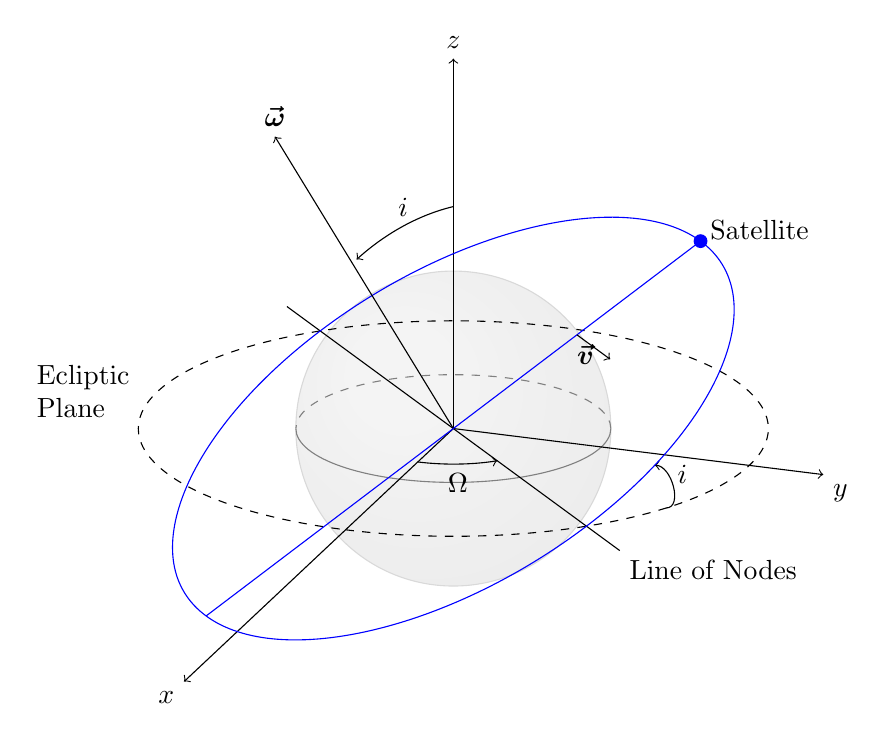
\begin{tikzpicture}[scale=5]
  \pgfmathsetmacro{\r}{.8}
  \pgfmathsetmacro{\O}{45} % right ascension of ascending node [deg]
  \pgfmathsetmacro{\i}{30} % inclination [deg]
  \pgfmathsetmacro{\f}{35} % true anomaly [deg]

  \coordinate (O) at (0,0,0);

  \pgfmathsetmacro{\Re}{0.4}
  \fill[ball color=gray!10, opacity=0.045] (0,0,0) circle ({\Re}); % 3D lighting effect
  \tdplotsetmaincoords{70}{110}
  \begin{scope}[tdplot_main_coords, shift={(0,0)}]

    % ball perimeter, gray
    \pgfmathsetmacro{\thetavec}{70}
    \pgfmathsetmacro{\phivec}{20}
    \tdplotsetrotatedcoords{\phivec}{\thetavec}{0}
    \tdplotdrawarc[tdplot_rotated_coords,color=gray!30]{(O)}{\Re}{0}{360}{}{}

    % equator
    \pgfmathsetmacro{\thetavec}{0}
    \pgfmathsetmacro{\phivec}{0}
    \tdplotsetrotatedcoords{\phivec}{\thetavec}{0}
    \tdplotdrawarc[tdplot_rotated_coords,color=black!50]{(O)}{\Re}{-70}{110}{}{}
    \tdplotdrawarc[tdplot_rotated_coords,color=black!50, dashed]{(O)}{\Re}{110}{290}{}{}

    \draw [->] (O) -- (2,0,0) node[anchor=north east] {$x$};
    \draw [->] (O) -- (0,1,0) node[anchor=north west] {$y$};
    \draw [->] (O) -- (0,0,1) node[anchor=south] {$z$};

    \node at (0,-\r,0) [left,text width=4em] {Ecliptic Plane};

    \tdplotdrawarc[dashed]{(O)}{\r}{0}{360}{}{}

    \tdplotsetrotatedcoords{\O}{0}{0}

    \draw [tdplot_rotated_coords] (-1,0,0) -- (1,0,0) node [below right] {Line of Nodes};
    \tdplotdrawarc[->]{(O)}{.33*\r}{0}{\O}{anchor=north}{$\Omega$}

    \tdplotsetrotatedcoords{-\O}{\i}{0}
    \pgfmathsetmacro{\alpha}{62.5}
    \pgfmathsetmacro{\p}{45}
    \path ({\r * cos(\alpha)},{\r * sin(\alpha)},{0}) coordinate (I1);
    \path[tdplot_rotated_coords] ({\r * cos(\alpha+\p)},{\r * sin(\alpha+\p)},{0}) coordinate (I2);
    \draw[->] (I1) to[out=360,in=0] node[pos=0.7,right] {$i$} (I2);
    \tdplotdrawarc[tdplot_rotated_coords,color=blue]{(O)}{\r}{0}{360}{}{} 
 
    \begin{scope}[tdplot_rotated_coords]
      \draw[->] (O) -- (0,0,1) node [above] {$\bm{\vec{\omega}}$};
      \draw[color=blue] (-\r,0,0) -- (\r,0,0);
      \fill[color=blue] (-\r,0,0) circle (0.5pt);
      \node[yshift=4pt,right] at (-\r,0,0) {Satellite};
      %\fill (-\r,0,0) circle[color=blue,radius=0.5pt] \node {Satellite};
      \coordinate (P) at (180:\Re);
      %\draw (O) -- (P);
      %\tdplotdrawarc[->]{(O)}{.33*\r}{180}{180+\f}{anchor=south west}{$\nu$}
    \end{scope}

    \tdplotsetrotatedcoords{-\O}{\i}{0}
    \tdplotsetrotatedcoordsorigin{(P)}
    \begin{scope}[tdplot_rotated_coords,scale=.2]
      %\draw [->] (P) -- (-1,0,0) node [right] {$\hat{r}$};
      \draw [->] (P) -- (0,1,0) node [pos=0.8,left] {$\bm{\vec{v}}$};
      %\draw [->] (P) -- (0,0,1) node [above] {$\hat{k}$};
      
    \end{scope}

  \end{scope}

  \tdplotsetthetaplanecoords{-\f}
  \tdplotdrawarc[tdplot_rotated_coords,->]{(O)}{.75*\r}{0}{\i}{anchor=south}{$i$} % not accurate :(
\end{tikzpicture}

  \caption{Geometry of a circular Earth orbit.}
  \label{fig-orbit-geometry}
\end{figure}

In addition to being aligned along the line-of-sight of the VSAT's main lobe, the eavesdropper needs to be able to intercept sufficiently long transmission to be able to %ilmaista lähettäjän olemus. 
This time dimension brings another point to consider when evaluating the risk of eavesdropping.
Different durations of interception have varying implications for the legitimate transmitter.
As an practical example, millisecond-level signal capture may be enough for DF applications, while in COMINT monitoring the signal for longer periods ranging all the way from seconds to days would be useful for gathering enough data. % TODO: parempi ilmaus tähän

Maximum duration of signal interception is set by the ability of the airborne platform to track the main lobe of the earth station.
The beam movement is primarily driven by the motion of the receiving satellite in orbit, which is in turn governed by Kepler's laws of orbital motion.
Tracking capability of the aircraft can be evaluated by analysing the velocity of the sub-satellite point at the eavesdropper's operational altitude (point x on figure \ref{fig-orbit-geometry}).
If this velocity exceeds the cruise speed of the eavesdropper, the airborne platform is not able to continuously follow the uplink RF beam, which limits the time window into individual satellite passes.

Communication satellites reside often in circular orbits, which are a special case when evaluating Kepler's laws of orbital motion.
Here, the velocity of the sub-satellite point can be computed by solving Kepler's third law for the orbital velocity at a set altitude.
In equatorial orbits, Earth's rotation can be directly substracted from the angular velocity of the satellite, as both share roughly the same rotational axis.

\begin{equation} \label{eq-kepler-3}
  T^2 = (\frac{4\pi^2}{GM})r^3
\end{equation}

where $T$ is the orbital period, $G$ is the gravitational constant, $M$ is the mass of the orbited body and $r$ is the radius of the orbit %measured from the centre of mass of the orbited body.

In essence, the aircraft can be modeled as a low-flying athmospheric satellite.
This allows for the same equations to be used in modeling its kinematic characteristics.
Solving the required velocity for successful beam tracking can be computed by equating the required orbital period of the aircraft to the one of the space-borne satellite.

Orbital period is related to the angular velocity of the satellite $\omega_{sat}$ through the equation

\begin{equation} \label{eq-ang-vel-1}
  \omega_{sat} = \frac{2\pi}{T}
\end{equation}

\noindent
which can be used to solve the tangential velocity component at a set altitude $v_r$

\begin{equation} \label{eq-ang-vel-2}
  v_r = \omega r
\end{equation}

\noindent
As $\omega_{sat} = \omega_{air}$ in the case that the aircraft is able to continuosly track the satellite, the velocity of the sub-satellite point at the cruising altitude of the aircraft $v_{r, air}$ can be solved by combining equations (\ref{eq-kepler-3}), (\ref{eq-ang-vel-1}) and (\ref{eq-ang-vel-2}).
Rearranging Kepler's third law to solve for $v_{r, air}$ gives

\begin{equation} \label{eq-v-air-equatorial}
  v_{r, air} = r_{air} \sqrt{\frac{G M_E}{r_{sat}^3}}
\end{equation}

\noindent
Variables $r_{air}$ and $r_{sat}$ are the orbital radiuses of the eavesdropping aircraft and the receiving satellite measured from the center of the Earth while $M_E$ is the mass of the Earth.
Equation (\ref{eq-v-air-equatorial}) gives $v_{r, air}$ in the ECI coordinate frame.
To compute the actual movement of the sub-satellite point relative to the surface of the Earth, the velocity figure needs to be converted to the ECF coordinate system.
For circular equatorial orbits, this can be simply achieved by substracting the spin of the Earth from $v_{r, air}$.

\begin{equation}
  v_{r, ECF} = v_{r, air} - \omega_E r_{air}
\end{equation}

\noindent
$\omega_E$ is the angular velocity of the Earth at the equator.

\begin{figure}[h]
  \centering
  % This file was created by matlab2tikz.
%
%The latest updates can be retrieved from
%  http://www.mathworks.com/matlabcentral/fileexchange/22022-matlab2tikz-matlab2tikz
%where you can also make suggestions and rate matlab2tikz.
%
\definecolor{mycolor1}{rgb}{0.00000,0.44700,0.74100}%
%
\begin{tikzpicture}

\begin{axis}[%
width=4.521in,
height=3.566in,
at={(0.758in,0.481in)},
scale only axis,
xmin=0,
xmax=40000000,
ymin=0,
ymax=8000,
axis background/.style={fill=white}
]
\addplot [color=mycolor1, forget plot]
  table[row sep=crcr]{%
500000	7072.71764129545\\
1000000	6365.41441116611\\
1500000	5768.61401343729\\
2000000	5259.57169914256\\
2500000	4821.22680484161\\
3000000	4440.55812330651\\
3500000	4107.47348810996\\
4000000	3814.04289796006\\
4500000	3553.95812701838\\
5000000	3322.14500116304\\
5500000	3114.480651329\\
6000000	2927.58426192998\\
6500000	2758.66012043392\\
7000000	2605.37844395658\\
7500000	2465.78386645891\\
8000000	2338.22443445674\\
8500000	2221.29598506997\\
9000000	2113.7981854881\\
9500000	2014.69950110221\\
10000000	1923.10906331822\\
10500000	1838.25391523213\\
11000000	1759.46048288005\\
11500000	1686.13939180947\\
12000000	1617.77295091573\\
12500000	1553.90477714283\\
13000000	1494.13114936631\\
13500000	1438.093767251\\
14000000	1385.47365808604\\
14500000	1335.98602660745\\
15000000	1289.37588333773\\
15500000	1245.41431874345\\
16000000	1203.89531557571\\
16500000	1164.63301164729\\
17000000	1127.45934116856\\
17500000	1092.22199549238\\
18000000	1058.7826543787\\
18500000	1027.01544720074\\
19000000	996.805610277406\\
19500000	968.048312044218\\
20000000	940.647622311633\\
20500000	914.515605598319\\
21000000	889.57152161971\\
21500000	865.741118580401\\
22000000	842.956007059067\\
22500000	821.153104064185\\
23000000	800.274138340326\\
23500000	780.265209268467\\
24000000	761.076392770707\\
24500000	742.661388533194\\
25000000	724.977203628275\\
25500000	707.983868270195\\
26000000	691.644179996502\\
26500000	675.923473044846\\
27000000	660.789410104709\\
27500000	646.211793976132\\
28000000	632.162396971571\\
28500000	618.614806159755\\
29000000	605.544282778029\\
29500000	592.927634337247\\
30000000	580.743098115126\\
30500000	568.970234883794\\
31000000	557.589831848052\\
31500000	546.583813885374\\
32000000	535.935162279006\\
32500000	525.627840223627\\
33000000	515.646724460593\\
33500000	505.97754246809\\
34000000	496.606814691834\\
34500000	487.521801355257\\
35000000	478.710453435377\\
35500000	470.161367432379\\
36000000	461.863743598168\\
36500000	453.807347322214\\
37000000	445.982473402509\\
};
\end{axis}
\end{tikzpicture}%
  \caption{Sub-satellite velocity as a function of orbital altitude (m) in equatiorial orbits.}
  \label{fig-subsat-velocity-equatiorial}
\end{figure}

Figure \ref{fig-subsat-velocity-equatiorial} shows the sub-satellite velocity ($v_{r, air}$) of a satellite in equatorial orbit as a function of orbital height $h_{sat} = r_{sat} - R_{E}$, where $R_{E}$ is the radius of the Earth.
Velocities are examined in orbits ranging from LEO to GEO, which corresponds to the range $h_{sat} = [5 \cdot 10^5, 3.7 \cdot 10^7]$.
In the resulting graph, the dependent variable or the sub-satellite velocity ($v_{r, air}$) is on the vertical axis, while the independent variable of the orbital height $h_{sat}$ is on the horizontal axis.
The graph can be observed approaching the rotational velocity of the Earth when $h_{sat}$ approaches the height of GEO 36000 km.
As the graph is computed in the ECF coordinate frame, we can se sub-satellite velocity approaching zero, which means that the satellite appears fixed in its position in the sky.
Cubically decreasing nature of $v_{sat}$ leads to radically higher values for LEO with $v_{sat}$ values ranging roughly between 5 and 7\ km/s in orbital altitudes between $h_{sat} = [5 \cdot 10^5, 2 \cdot 10^6]$.

\subsection{Submodel 2b: Beam tracking potential in inclined orbits} \label{ch-results-submodel-2b-tracking-inclined}

Circular equatorial orbits are a good starting point for listening window analysis but their real world applications are somewhat in limited when considering relationship of orbital altitude to coverage and latency.
As discussed in chapter \ref{ch-constellation-characteristics}, modern satellite megaconstellations, such as the systems in appendix \ref{appendix-constellation-comparison}, aim to achieve worldwide coverage by placing a number of satellites into inclined circular Earth orbits.
Common configurations include the Walker Star and Delta constellation configurations, the advantages and disadvantages of which are discussed in more detail in the aforementioned chapter.

The same analysis methods remain valid for inclined orbits but some additional factors need to be considered.
Equatorial orbits have only a single velocity component parallel to the xy-plane in both ECI and ECF coordinate frames.
On the other hand, any inclination induces additional velocity component perpendicular to this original equatorial component.
This velocity component is visualised by $v_z$ in figure \ref{fig-inclined-v-components}. % TODO: Kuvaaja puuttuu

Transitioning from the simple scalar representation into a vector space makes analyzing inclined orbital motion less cumbersome.
Here, angular velocity is a very useful abstraction, as it allows to sum different rotational speed components together.
As angular velocity does not vary in in circular motion, examining the magnitude of the sum of the angular velocity vectors allows us to gauge the tracking potential of differently inclined orbits at the desired range of altitudes.

The ECI coordinate frame is a natural starting point for evaluating orbital motion.
Angular velocity pseudovector of a circular orbit follows the right hand rule, being perpendicular to the rotational plane.
Rotational motion in the equatorial plane can be represented with angular velocity pseudovector $\bm{\vec{\omega}} = [0,0,\omega]^T$.
Inclined orbits can be generated by rotating this equatorial orbit about its diameter, which can be achieved with multiplying the pseudovector with a suitable three-dimensional rotational matrix.
To rotate the orbits about the y-axis of the ECI coordinate frame by $\theta$ degrees, rotation matrix $\bm{R_y}$ can be used.

\begin{equation*}
  \bm{R_y}(\theta) = \begin{bmatrix}
    \cos \theta & -\sin \theta & 0 \\[3pt]
    \sin \theta &  \cos \theta & 0 \\[3pt]
    0           &  0           & 1 \\
    \end{bmatrix}
\end{equation*}

Multiplying the vector by matrix $\bm{R_y}(\theta)$ and substracting the rotation vector of the Earth gives angular velocity vector in the ECF coordinate frame.
This can be in turn be converted to the velocity of the sub-satellite by taking the norm of the angular velocity pseudovector

\begin{equation*}
  \omega_{ECF} =
  ||\bm{R_y}(\theta)\ \bm{\vec{\omega_{sat, i}}} - \bm{\vec{\omega_{E}}}||
\end{equation*}

$\omega_{ECF}$ is the scalar angular velocity of the satellite in the ECF coordinate frame.
$\bm{\vec{\omega_{sat, i}}}$ and $\bm{\vec{\omega_{E}}}$ are the angular velocity vectors of the inclined satellite orbit and the spin of the Earth.
Finally, the sub-satellite velocity figure can be solved based on the scalar angular velocity by applying equation (\ref{eq-ang-vel-2}), as the altitude of the airborne platform $h_{air}$ and the mean radius of the Earth $R_E$ are known.

\begin{equation}
  v_{air} = \omega_{ECF}\ (h_{air} + R_E)
\end{equation}

\begin{figure}[h]
  \centering
  % This file was created by matlab2tikz.
%
%The latest updates can be retrieved from
%  http://www.mathworks.com/matlabcentral/fileexchange/22022-matlab2tikz-matlab2tikz
%where you can also make suggestions and rate matlab2tikz.
%
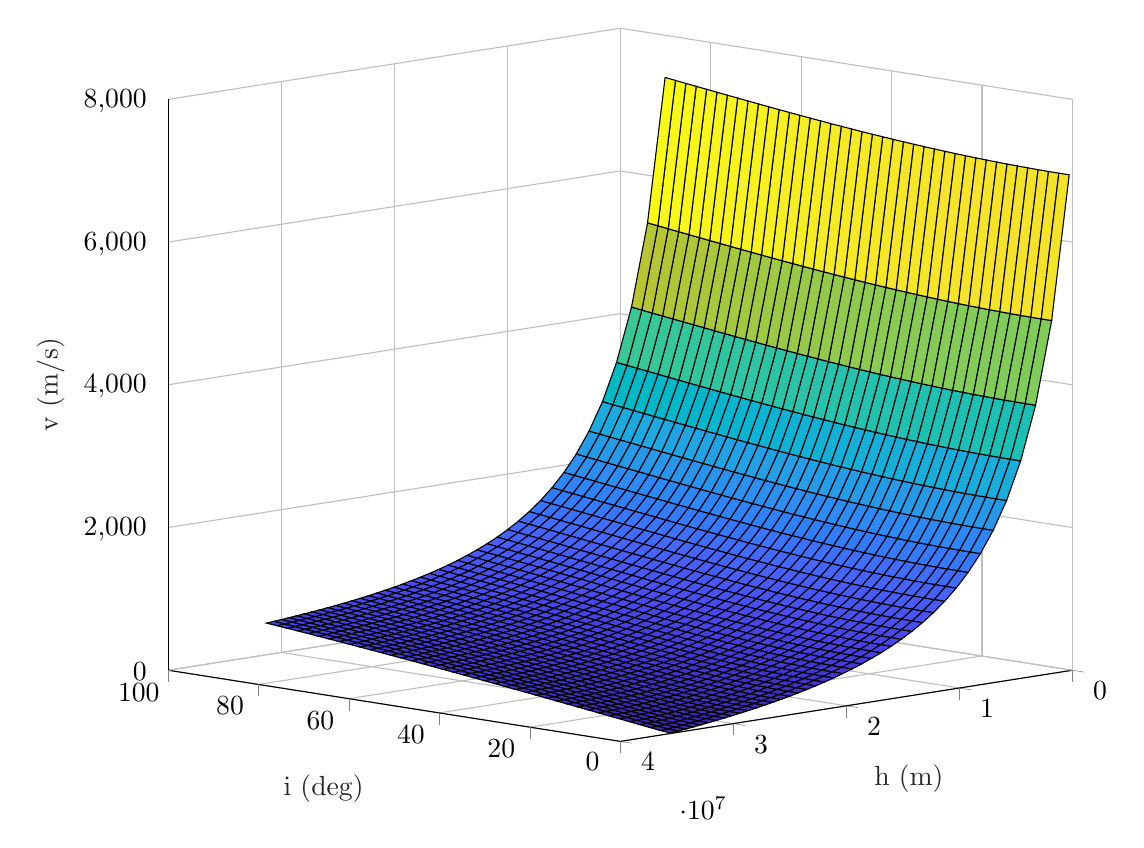
\begin{tikzpicture}

\begin{axis}[%
width=4.521in,
height=3.566in,
at={(0.758in,0.481in)},
scale only axis,
xmin=0,
xmax=100,
tick align=outside,
xlabel style={font=\color{white!15!black}},
xlabel={i (deg)},
ymin=0,
ymax=40000000,
ylabel style={font=\color{white!15!black}},
ylabel={h (m)},
zmin=0,
zmax=8000,
zlabel style={font=\color{white!15!black}},
zlabel={v (m/s)},
view={-135}{10},
axis background/.style={fill=white},
axis x line*=bottom,
axis y line*=left,
axis z line*=left,
xmajorgrids,
ymajorgrids,
zmajorgrids
]

\addplot3[%
surf,
shader=flat corner, draw=black, z buffer=sort, colormap={mymap}{[1pt] rgb(0pt)=(0.2422,0.1504,0.6603); rgb(1pt)=(0.2444,0.1534,0.6728); rgb(2pt)=(0.2464,0.1569,0.6847); rgb(3pt)=(0.2484,0.1607,0.6961); rgb(4pt)=(0.2503,0.1648,0.7071); rgb(5pt)=(0.2522,0.1689,0.7179); rgb(6pt)=(0.254,0.1732,0.7286); rgb(7pt)=(0.2558,0.1773,0.7393); rgb(8pt)=(0.2576,0.1814,0.7501); rgb(9pt)=(0.2594,0.1854,0.761); rgb(11pt)=(0.2628,0.1932,0.7828); rgb(12pt)=(0.2645,0.1972,0.7937); rgb(13pt)=(0.2661,0.2011,0.8043); rgb(14pt)=(0.2676,0.2052,0.8148); rgb(15pt)=(0.2691,0.2094,0.8249); rgb(16pt)=(0.2704,0.2138,0.8346); rgb(17pt)=(0.2717,0.2184,0.8439); rgb(18pt)=(0.2729,0.2231,0.8528); rgb(19pt)=(0.274,0.228,0.8612); rgb(20pt)=(0.2749,0.233,0.8692); rgb(21pt)=(0.2758,0.2382,0.8767); rgb(22pt)=(0.2766,0.2435,0.884); rgb(23pt)=(0.2774,0.2489,0.8908); rgb(24pt)=(0.2781,0.2543,0.8973); rgb(25pt)=(0.2788,0.2598,0.9035); rgb(26pt)=(0.2794,0.2653,0.9094); rgb(27pt)=(0.2798,0.2708,0.915); rgb(28pt)=(0.2802,0.2764,0.9204); rgb(29pt)=(0.2806,0.2819,0.9255); rgb(30pt)=(0.2809,0.2875,0.9305); rgb(31pt)=(0.2811,0.293,0.9352); rgb(32pt)=(0.2813,0.2985,0.9397); rgb(33pt)=(0.2814,0.304,0.9441); rgb(34pt)=(0.2814,0.3095,0.9483); rgb(35pt)=(0.2813,0.315,0.9524); rgb(36pt)=(0.2811,0.3204,0.9563); rgb(37pt)=(0.2809,0.3259,0.96); rgb(38pt)=(0.2807,0.3313,0.9636); rgb(39pt)=(0.2803,0.3367,0.967); rgb(40pt)=(0.2798,0.3421,0.9702); rgb(41pt)=(0.2791,0.3475,0.9733); rgb(42pt)=(0.2784,0.3529,0.9763); rgb(43pt)=(0.2776,0.3583,0.9791); rgb(44pt)=(0.2766,0.3638,0.9817); rgb(45pt)=(0.2754,0.3693,0.984); rgb(46pt)=(0.2741,0.3748,0.9862); rgb(47pt)=(0.2726,0.3804,0.9881); rgb(48pt)=(0.271,0.386,0.9898); rgb(49pt)=(0.2691,0.3916,0.9912); rgb(50pt)=(0.267,0.3973,0.9924); rgb(51pt)=(0.2647,0.403,0.9935); rgb(52pt)=(0.2621,0.4088,0.9946); rgb(53pt)=(0.2591,0.4145,0.9955); rgb(54pt)=(0.2556,0.4203,0.9965); rgb(55pt)=(0.2517,0.4261,0.9974); rgb(56pt)=(0.2473,0.4319,0.9983); rgb(57pt)=(0.2424,0.4378,0.9991); rgb(58pt)=(0.2369,0.4437,0.9996); rgb(59pt)=(0.2311,0.4497,0.9995); rgb(60pt)=(0.225,0.4559,0.9985); rgb(61pt)=(0.2189,0.462,0.9968); rgb(62pt)=(0.2128,0.4682,0.9948); rgb(63pt)=(0.2066,0.4743,0.9926); rgb(64pt)=(0.2006,0.4803,0.9906); rgb(65pt)=(0.195,0.4861,0.9887); rgb(66pt)=(0.1903,0.4919,0.9867); rgb(67pt)=(0.1869,0.4975,0.9844); rgb(68pt)=(0.1847,0.503,0.9819); rgb(69pt)=(0.1831,0.5084,0.9793); rgb(70pt)=(0.1818,0.5138,0.9766); rgb(71pt)=(0.1806,0.5191,0.9738); rgb(72pt)=(0.1795,0.5244,0.9709); rgb(73pt)=(0.1785,0.5296,0.9677); rgb(74pt)=(0.1778,0.5349,0.9641); rgb(75pt)=(0.1773,0.5401,0.9602); rgb(76pt)=(0.1768,0.5452,0.956); rgb(77pt)=(0.1764,0.5504,0.9516); rgb(78pt)=(0.1755,0.5554,0.9473); rgb(79pt)=(0.174,0.5605,0.9432); rgb(80pt)=(0.1716,0.5655,0.9393); rgb(81pt)=(0.1686,0.5705,0.9357); rgb(82pt)=(0.1649,0.5755,0.9323); rgb(83pt)=(0.161,0.5805,0.9289); rgb(84pt)=(0.1573,0.5854,0.9254); rgb(85pt)=(0.154,0.5902,0.9218); rgb(86pt)=(0.1513,0.595,0.9182); rgb(87pt)=(0.1492,0.5997,0.9147); rgb(88pt)=(0.1475,0.6043,0.9113); rgb(89pt)=(0.1461,0.6089,0.908); rgb(90pt)=(0.1446,0.6135,0.905); rgb(91pt)=(0.1429,0.618,0.9022); rgb(92pt)=(0.1408,0.6226,0.8998); rgb(93pt)=(0.1383,0.6272,0.8975); rgb(94pt)=(0.1354,0.6317,0.8953); rgb(95pt)=(0.1321,0.6363,0.8932); rgb(96pt)=(0.1288,0.6408,0.891); rgb(97pt)=(0.1253,0.6453,0.8887); rgb(98pt)=(0.1219,0.6497,0.8862); rgb(99pt)=(0.1185,0.6541,0.8834); rgb(100pt)=(0.1152,0.6584,0.8804); rgb(101pt)=(0.1119,0.6627,0.877); rgb(102pt)=(0.1085,0.6669,0.8734); rgb(103pt)=(0.1048,0.671,0.8695); rgb(104pt)=(0.1009,0.675,0.8653); rgb(105pt)=(0.0964,0.6789,0.8609); rgb(106pt)=(0.0914,0.6828,0.8562); rgb(107pt)=(0.0855,0.6865,0.8513); rgb(108pt)=(0.0789,0.6902,0.8462); rgb(109pt)=(0.0713,0.6938,0.8409); rgb(110pt)=(0.0628,0.6972,0.8355); rgb(111pt)=(0.0535,0.7006,0.8299); rgb(112pt)=(0.0433,0.7039,0.8242); rgb(113pt)=(0.0328,0.7071,0.8183); rgb(114pt)=(0.0234,0.7103,0.8124); rgb(115pt)=(0.0155,0.7133,0.8064); rgb(116pt)=(0.0091,0.7163,0.8003); rgb(117pt)=(0.0046,0.7192,0.7941); rgb(118pt)=(0.0019,0.722,0.7878); rgb(119pt)=(0.0009,0.7248,0.7815); rgb(120pt)=(0.0018,0.7275,0.7752); rgb(121pt)=(0.0046,0.7301,0.7688); rgb(122pt)=(0.0094,0.7327,0.7623); rgb(123pt)=(0.0162,0.7352,0.7558); rgb(124pt)=(0.0253,0.7376,0.7492); rgb(125pt)=(0.0369,0.74,0.7426); rgb(126pt)=(0.0504,0.7423,0.7359); rgb(127pt)=(0.0638,0.7446,0.7292); rgb(128pt)=(0.077,0.7468,0.7224); rgb(129pt)=(0.0899,0.7489,0.7156); rgb(130pt)=(0.1023,0.751,0.7088); rgb(131pt)=(0.1141,0.7531,0.7019); rgb(132pt)=(0.1252,0.7552,0.695); rgb(133pt)=(0.1354,0.7572,0.6881); rgb(134pt)=(0.1448,0.7593,0.6812); rgb(135pt)=(0.1532,0.7614,0.6741); rgb(136pt)=(0.1609,0.7635,0.6671); rgb(137pt)=(0.1678,0.7656,0.6599); rgb(138pt)=(0.1741,0.7678,0.6527); rgb(139pt)=(0.1799,0.7699,0.6454); rgb(140pt)=(0.1853,0.7721,0.6379); rgb(141pt)=(0.1905,0.7743,0.6303); rgb(142pt)=(0.1954,0.7765,0.6225); rgb(143pt)=(0.2003,0.7787,0.6146); rgb(144pt)=(0.2061,0.7808,0.6065); rgb(145pt)=(0.2118,0.7828,0.5983); rgb(146pt)=(0.2178,0.7849,0.5899); rgb(147pt)=(0.2244,0.7869,0.5813); rgb(148pt)=(0.2318,0.7887,0.5725); rgb(149pt)=(0.2401,0.7905,0.5636); rgb(150pt)=(0.2491,0.7922,0.5546); rgb(151pt)=(0.2589,0.7937,0.5454); rgb(152pt)=(0.2695,0.7951,0.536); rgb(153pt)=(0.2809,0.7964,0.5266); rgb(154pt)=(0.2929,0.7975,0.517); rgb(155pt)=(0.3052,0.7985,0.5074); rgb(156pt)=(0.3176,0.7994,0.4975); rgb(157pt)=(0.3301,0.8002,0.4876); rgb(158pt)=(0.3424,0.8009,0.4774); rgb(159pt)=(0.3548,0.8016,0.4669); rgb(160pt)=(0.3671,0.8021,0.4563); rgb(161pt)=(0.3795,0.8026,0.4454); rgb(162pt)=(0.3921,0.8029,0.4344); rgb(163pt)=(0.405,0.8031,0.4233); rgb(164pt)=(0.4184,0.803,0.4122); rgb(165pt)=(0.4322,0.8028,0.4013); rgb(166pt)=(0.4463,0.8024,0.3904); rgb(167pt)=(0.4608,0.8018,0.3797); rgb(168pt)=(0.4753,0.8011,0.3691); rgb(169pt)=(0.4899,0.8002,0.3586); rgb(170pt)=(0.5044,0.7993,0.348); rgb(171pt)=(0.5187,0.7982,0.3374); rgb(172pt)=(0.5329,0.797,0.3267); rgb(173pt)=(0.547,0.7957,0.3159); rgb(175pt)=(0.5748,0.7929,0.2941); rgb(176pt)=(0.5886,0.7913,0.2833); rgb(177pt)=(0.6024,0.7896,0.2726); rgb(178pt)=(0.6161,0.7878,0.2622); rgb(179pt)=(0.6297,0.7859,0.2521); rgb(180pt)=(0.6433,0.7839,0.2423); rgb(181pt)=(0.6567,0.7818,0.2329); rgb(182pt)=(0.6701,0.7796,0.2239); rgb(183pt)=(0.6833,0.7773,0.2155); rgb(184pt)=(0.6963,0.775,0.2075); rgb(185pt)=(0.7091,0.7727,0.1998); rgb(186pt)=(0.7218,0.7703,0.1924); rgb(187pt)=(0.7344,0.7679,0.1852); rgb(188pt)=(0.7468,0.7654,0.1782); rgb(189pt)=(0.759,0.7629,0.1717); rgb(190pt)=(0.771,0.7604,0.1658); rgb(191pt)=(0.7829,0.7579,0.1608); rgb(192pt)=(0.7945,0.7554,0.157); rgb(193pt)=(0.806,0.7529,0.1546); rgb(194pt)=(0.8172,0.7505,0.1535); rgb(195pt)=(0.8281,0.7481,0.1536); rgb(196pt)=(0.8389,0.7457,0.1546); rgb(197pt)=(0.8495,0.7435,0.1564); rgb(198pt)=(0.86,0.7413,0.1587); rgb(199pt)=(0.8703,0.7392,0.1615); rgb(200pt)=(0.8804,0.7372,0.165); rgb(201pt)=(0.8903,0.7353,0.1695); rgb(202pt)=(0.9,0.7336,0.1749); rgb(203pt)=(0.9093,0.7321,0.1815); rgb(204pt)=(0.9184,0.7308,0.189); rgb(205pt)=(0.9272,0.7298,0.1973); rgb(206pt)=(0.9357,0.729,0.2061); rgb(207pt)=(0.944,0.7285,0.2151); rgb(208pt)=(0.9523,0.7284,0.2237); rgb(209pt)=(0.9606,0.7285,0.2312); rgb(210pt)=(0.9689,0.7292,0.2373); rgb(211pt)=(0.977,0.7304,0.2418); rgb(212pt)=(0.9842,0.733,0.2446); rgb(213pt)=(0.99,0.7365,0.2429); rgb(214pt)=(0.9946,0.7407,0.2394); rgb(215pt)=(0.9966,0.7458,0.2351); rgb(216pt)=(0.9971,0.7513,0.2309); rgb(217pt)=(0.9972,0.7569,0.2267); rgb(218pt)=(0.9971,0.7626,0.2224); rgb(219pt)=(0.9969,0.7683,0.2181); rgb(220pt)=(0.9966,0.774,0.2138); rgb(221pt)=(0.9962,0.7798,0.2095); rgb(222pt)=(0.9957,0.7856,0.2053); rgb(223pt)=(0.9949,0.7915,0.2012); rgb(224pt)=(0.9938,0.7974,0.1974); rgb(225pt)=(0.9923,0.8034,0.1939); rgb(226pt)=(0.9906,0.8095,0.1906); rgb(227pt)=(0.9885,0.8156,0.1875); rgb(228pt)=(0.9861,0.8218,0.1846); rgb(229pt)=(0.9835,0.828,0.1817); rgb(230pt)=(0.9807,0.8342,0.1787); rgb(231pt)=(0.9778,0.8404,0.1757); rgb(232pt)=(0.9748,0.8467,0.1726); rgb(233pt)=(0.972,0.8529,0.1695); rgb(234pt)=(0.9694,0.8591,0.1665); rgb(235pt)=(0.9671,0.8654,0.1636); rgb(236pt)=(0.9651,0.8716,0.1608); rgb(237pt)=(0.9634,0.8778,0.1582); rgb(238pt)=(0.9619,0.884,0.1557); rgb(239pt)=(0.9608,0.8902,0.1532); rgb(240pt)=(0.9601,0.8963,0.1507); rgb(241pt)=(0.9596,0.9023,0.148); rgb(242pt)=(0.9595,0.9084,0.145); rgb(243pt)=(0.9597,0.9143,0.1418); rgb(244pt)=(0.9601,0.9203,0.1382); rgb(245pt)=(0.9608,0.9262,0.1344); rgb(246pt)=(0.9618,0.932,0.1304); rgb(247pt)=(0.9629,0.9379,0.1261); rgb(248pt)=(0.9642,0.9437,0.1216); rgb(249pt)=(0.9657,0.9494,0.1168); rgb(250pt)=(0.9674,0.9552,0.1116); rgb(251pt)=(0.9692,0.9609,0.1061); rgb(252pt)=(0.9711,0.9667,0.1001); rgb(253pt)=(0.973,0.9724,0.0938); rgb(254pt)=(0.9749,0.9782,0.0872); rgb(255pt)=(0.9769,0.9839,0.0805)}, mesh/rows=40]
table[row sep=crcr, point meta=\thisrow{c}] {%
%
x	y	z	c\\
0	281546.901327529	6949.69251459581	6949.69251459581\\
0	1836546.6625824	4946.17755543305	4946.17755543305\\
0	3255701.78304605	3795.22215336083	3795.22215336083\\
0	4576851.50661658	3048.1107520157	3048.1107520157\\
0	5822514.48405775	2524.01767943032	2524.01767943032\\
0	7007462.56915398	2136.05267764633	2136.05267764633\\
0	8142046.33651562	1837.27503259429	1837.27503259429\\
0	9233873.58196417	1600.10102569732	1600.10102569732\\
0	10288743.0632444	1407.25860887454	1407.25860887454\\
0	11311202.8495916	1247.38070774797	1247.38070774797\\
0	12304903.4233899	1112.68042884605	1112.68042884605\\
0	13272831.2041727	997.644424236381	997.644424236381\\
0	14217468.7555663	898.259576716465	898.259576716465\\
0	15140908.1083929	811.535219326474	811.535219326474\\
0	16044933.0269694	735.197012522111	735.197012522111\\
0	16931080.0757445	667.484591797337	667.484591797337\\
0	17800684.8353919	607.014141203555	607.014141203555\\
0	18654917.4786671	552.682822649751	552.682822649751\\
0	19494810.5699212	503.600906854769	503.600906854769\\
0	20321281.0804964	459.0426699349	459.0426699349\\
0	21135148.0337524	418.410268867002	418.410268867002\\
0	21937146.8010128	381.20676240399	381.20676240399\\
0	22727940.7981413	347.015685614096	347.015685614096\\
0	23508131.1411504	315.485393010186	315.485393010186\\
0	24278264.6822812	286.316920076981	286.316920076981\\
0	25038840.7484865	259.254474070361	259.254474070361\\
0	25790316.8309764	234.077912802878	234.077912802878\\
0	26533113.4198486	210.59674286654	210.59674286654\\
0	27267618.136637	188.645290841363	188.645290841363\\
0	27994189.2862084	168.078788470771	168.078788470771\\
0	28713158.9252824	148.770176153427	148.770176153427\\
0	29424835.5260808	130.607475546311	130.607475546311\\
0	30129506.2989211	113.491616472746	113.491616472746\\
0	30827439.2259617	97.3346290559636	97.3346290559636\\
0	31518884.8490843	82.0581314166625	82.0581314166625\\
0	32204077.8475048	67.5920580553085	67.5920580553085\\
0	32883238.4347494	53.8735853844636	53.8735853844636\\
0	33556573.5997965	40.8462196491777	40.8462196491777\\
0	34224278.2132461	28.4590193062891	28.4590193062891\\
0	34886536.0161399	16.6659292915967	16.6659292915967\\
0	35543520.5063905	5.42520883262747	5.42520883262747\\
2.29183118052329	281546.901327529	6950.08781092702	6950.08781092702\\
2.29183118052329	1836546.6625824	4946.58285418764	4946.58285418764\\
2.29183118052329	3255701.78304605	3795.63797361308	3795.63797361308\\
2.29183118052329	4576851.50661658	3048.53765430012	3048.53765430012\\
2.29183118052329	5822514.48405775	2524.45627027531	2524.45627027531\\
2.29183118052329	7007462.56915398	2136.50361474458	2136.50361474458\\
2.29183118052329	8142046.33651562	1837.73903072023	1837.73903072023\\
2.29183118052329	9233873.58196417	1600.5788635049	1600.5788635049\\
2.29183118052329	10288743.0632444	1407.75113673736	1407.75113673736\\
2.29183118052329	11311202.8495916	1247.88885683923	1247.88885683923\\
2.29183118052329	12304903.4233899	1113.20522170128	1113.20522170128\\
2.29183118052329	13272831.2041727	998.186987098976	998.186987098976\\
2.29183118052329	14217468.7555663	898.821154039383	898.821154039383\\
2.29183118052329	15140908.1083929	812.117190897951	812.117190897951\\
2.29183118052329	16044933.0269694	735.800913805821	735.800913805821\\
2.29183118052329	16931080.0757445	668.112138238443	668.112138238443\\
2.29183118052329	17800684.8353919	607.667257464963	607.667257464963\\
2.29183118052329	18654917.4786671	553.363678027675	553.363678027675\\
2.29183118052329	19494810.5699212	504.311958507563	504.311958507563\\
2.29183118052329	20321281.0804964	459.786716085613	459.786716085613\\
2.29183118052329	21135148.0337524	419.190514869358	419.190514869358\\
2.29183118052329	21937146.8010128	382.026903585825	382.026903585825\\
2.29183118052329	22727940.7981413	347.880012272648	347.880012272648\\
2.29183118052329	23508131.1411504	316.398925050174	316.398925050174\\
2.29183118052329	24278264.6822812	287.285581905454	287.285581905454\\
2.29183118052329	25038840.7484865	260.285325062513	260.285325062513\\
2.29183118052329	25790316.8309764	235.179455883239	235.179455883239\\
2.29183118052329	26533113.4198486	211.779345145609	211.779345145609\\
2.29183118052329	27267618.136637	189.921768703247	189.921768703247\\
2.29183118052329	27994189.2862084	169.465240323871	169.465240323871\\
2.29183118052329	28713158.9252824	150.287199324064	150.287199324064\\
2.29183118052329	29424835.5260808	132.281999576515	132.281999576515\\
2.29183118052329	30129506.2989211	115.359765295938	115.359765295938\\
2.29183118052329	30827439.2259617	99.4463818671021	99.4463818671021\\
2.29183118052329	31518884.8490843	84.4853053410356	84.4853053410356\\
2.29183118052329	32204077.8475048	70.4428415167709	70.4428415167709\\
2.29183118052329	32883238.4347494	57.321048976057	57.321048976057\\
2.29183118052329	33556573.5997965	45.1895696763823	45.1895696763823\\
2.29183118052329	34224278.2132461	34.2697813507757	34.2697813507757\\
2.29183118052329	34886536.0161399	25.1697094686952	25.1697094686952\\
2.29183118052329	35543520.5063905	19.4129422125864	19.4129422125864\\
4.58366236104659	281546.901327529	6951.27293278139	6951.27293278139\\
4.58366236104659	1836546.6625824	4947.7979030455	4947.7979030455\\
4.58366236104659	3255701.78304605	3796.88449616679	3796.88449616679\\
4.58366236104659	4576851.50661658	3049.81731999797	3049.81731999797\\
4.58366236104659	5822514.48405775	2525.77088462673	2525.77088462673\\
4.58366236104659	7007462.56915398	2137.85513447261	2137.85513447261\\
4.58366236104659	8142046.33651562	1839.12958107669	1839.12958107669\\
4.58366236104659	9233873.58196417	1602.01075812823	1602.01075812823\\
4.58366236104659	10288743.0632444	1409.22690051297	1409.22690051297\\
4.58366236104659	11311202.8495916	1249.41125232198	1249.41125232198\\
4.58366236104659	12304903.4233899	1114.77727978458	1114.77727978458\\
4.58366236104659	13272831.2041727	999.812042772889	999.812042772889\\
4.58366236104659	14217468.7555663	900.502888280684	900.502888280684\\
4.58366236104659	15140908.1083929	813.859679991832	813.859679991832\\
4.58366236104659	16044933.0269694	737.608687730194	737.608687730194\\
4.58366236104659	16931080.0757445	669.990250172372	669.990250172372\\
4.58366236104659	17800684.8353919	609.621367047487	609.621367047487\\
4.58366236104659	18654917.4786671	555.400151740425	555.400151740425\\
4.58366236104659	19494810.5699212	506.437991552778	506.437991552778\\
4.58366236104659	20321281.0804964	462.010481478262	462.010481478262\\
4.58366236104659	21135148.0337524	421.52134730003	421.52134730003\\
4.58366236104659	21937146.8010128	384.475528147697	384.475528147697\\
4.58366236104659	22727940.7981413	350.4588316903	350.4588316903\\
4.58366236104659	23508131.1411504	319.122384065856	319.122384065856\\
4.58366236104659	24278264.6822812	290.170634681539	290.170634681539\\
4.58366236104659	25038840.7484865	263.352041952125	263.352041952125\\
4.58366236104659	25790316.8309764	238.451821444975	238.451821444975\\
4.58366236104659	26533113.4198486	215.286322615028	215.286322615028\\
4.58366236104659	27267618.136637	193.698741789259	193.698741789259\\
4.58366236104659	27994189.2862084	173.555998538986	173.555998538986\\
4.58366236104659	28713158.9252824	154.746720153123	154.746720153123\\
4.58366236104659	29424835.5260808	137.180419129051	137.180419129051\\
4.58366236104659	30129506.2989211	120.788148480897	120.788148480897\\
4.58366236104659	30827439.2259617	105.525241670065	105.525241670065\\
4.58366236104659	31518884.8490843	91.3772936669789	91.3772936669789\\
4.58366236104659	32204077.8475048	78.3714694205789	78.3714694205789\\
4.58366236104659	32883238.4347494	66.5966046805683	66.5966046805683\\
4.58366236104659	33556573.5997965	56.2365542800952	56.2365542800952\\
4.58366236104659	34224278.2132461	47.6166062423044	47.6166062423044\\
4.58366236104659	34886536.0161399	41.2338254309168	41.2338254309168\\
4.58366236104659	35543520.5063905	37.6642378893188	37.6642378893188\\
6.87549354156988	281546.901327529	6953.24558105936	6953.24558105936\\
6.87549354156988	1836546.6625824	4949.82016290485	4949.82016290485\\
6.87549354156988	3255701.78304605	3798.95891055346	3798.95891055346\\
6.87549354156988	4576851.50661658	3051.94663109814	3051.94663109814\\
6.87549354156988	5822514.48405775	2527.958055075	2527.958055075\\
6.87549354156988	7007462.56915398	2140.10337143484	2140.10337143484\\
6.87549354156988	8142046.33651562	1841.4423636834	1841.4423636834\\
6.87549354156988	9233873.58196417	1604.39186882829	1604.39186882829\\
6.87549354156988	10288743.0632444	1411.68046103214	1411.68046103214\\
6.87549354156988	11311202.8495916	1251.94176505266	1251.94176505266\\
6.87549354156988	12304903.4233899	1117.38967560931	1117.38967560931\\
6.87549354156988	13272831.2041727	1002.51173654327	1002.51173654327\\
6.87549354156988	14217468.7555663	903.295843448913	903.295843448913\\
6.87549354156988	15140908.1083929	816.752484238527	816.752484238527\\
6.87549354156988	16044933.0269694	740.608641872371	740.608641872371\\
6.87549354156988	16931080.0757445	673.105473196241	673.105473196241\\
6.87549354156988	17800684.8353919	612.860920830745	612.860920830745\\
6.87549354156988	18654917.4786671	558.774189958032	558.774189958032\\
6.87549354156988	19494810.5699212	509.957938467194	509.957938467194\\
6.87549354156988	20321281.0804964	465.689247891831	465.689247891831\\
6.87549354156988	21135148.0337524	425.373593018422	425.373593018422\\
6.87549354156988	21937146.8010128	388.517983037404	388.517983037404\\
6.87549354156988	22727940.7981413	354.710691036362	354.710691036362\\
6.87549354156988	23508131.1411504	323.605798747396	323.605798747396\\
6.87549354156988	24278264.6822812	294.911323067288	294.911323067288\\
6.87549354156988	25038840.7484865	268.380058842564	268.380058842564\\
6.87549354156988	25790316.8309764	243.802530347734	243.802530347734\\
6.87549354156988	26533113.4198486	221.001631474537	221.001631474537\\
6.87549354156988	27267618.136637	199.828678664694	199.828678664694\\
6.87549354156988	27994189.2862084	180.160720298651	180.160720298651\\
6.87549354156988	28713158.9252824	161.899056412169	161.899056412169\\
6.87549354156988	29424835.5260808	144.969034581755	144.969034581755\\
6.87549354156988	30129506.2989211	129.321306573199	129.321306573199\\
6.87549354156988	30827439.2259617	114.934842317042	114.934842317042\\
6.87549354156988	31518884.8490843	101.822035234926	101.822035234926\\
6.87549354156988	32204077.8475048	90.0359851899436	90.0359851899436\\
6.87549354156988	32883238.4347494	79.6789790158276	79.6789790158276\\
6.87549354156988	33556573.5997965	70.9082482043018	70.9082482043018\\
6.87549354156988	34224278.2132461	63.9291573884123	63.9291573884123\\
6.87549354156988	34886536.0161399	58.9592141989404	58.9592141989404\\
6.87549354156988	35543520.5063905	56.1512583333558	56.1512583333558\\
9.16732472209317	281546.901327529	6956.00193164115	6956.00193164115\\
9.16732472209317	1836546.6625824	4952.64541229004	4952.64541229004\\
9.16732472209317	3255701.78304605	3801.85654641746	3801.85654641746\\
9.16732472209317	4576851.50661658	3054.92040902971	3054.92040902971\\
9.16732472209317	5822514.48405775	2531.01202629999	2531.01202629999\\
9.16732472209317	7007462.56915398	2143.2419141555	2143.2419141555\\
9.16732472209317	8142046.33651562	1844.67021860216	1844.67021860216\\
9.16732472209317	9233873.58196417	1607.71417952918	1607.71417952918\\
9.16732472209317	10288743.0632444	1415.10282001917	1415.10282001917\\
9.16732472209317	11311202.8495916	1255.47026639738	1255.47026639738\\
9.16732472209317	12304903.4233899	1121.03097534556	1121.03097534556\\
9.16732472209317	13272831.2041727	1006.27312217368	1006.27312217368\\
9.16732472209317	14217468.7555663	907.185314204155	907.185314204155\\
9.16732472209317	15140908.1083929	820.778844069189	820.778844069189\\
9.16732472209317	16044933.0269694	744.78160756808	744.78160756808\\
9.16732472209317	16931080.0757445	677.435800535987	677.435800535987\\
9.16732472209317	17800684.8353919	617.360552292093	617.360552292093\\
9.16732472209317	18654917.4786671	563.456428275743	563.456428275743\\
9.16732472209317	19494810.5699212	514.837651259574	514.837651259574\\
9.16732472209317	20321281.0804964	470.783109691392	470.783109691392\\
9.16732472209317	21135148.0337524	430.700372370218	430.700372370218\\
9.16732472209317	21937146.8010128	394.098883861308	394.098883861308\\
9.16732472209317	22727940.7981413	360.569759138376	360.569759138376\\
9.16732472209317	23508131.1411504	329.770406061032	329.770406061032\\
9.16732472209317	24278264.6822812	301.41274356253	301.41274356253\\
9.16732472209317	25038840.7484865	275.254150327301	275.254150327301\\
9.16732472209317	25790316.8309764	251.09053414325	251.09053414325\\
9.16732472209317	26533113.4198486	228.751094330685	228.751094330685\\
9.16732472209317	27267618.136637	208.094482875396	208.094482875396\\
9.16732472209317	27994189.2862084	189.006168641576	189.006168641576\\
9.16732472209317	28713158.9252824	171.396879666721	171.396879666721\\
9.16732472209317	29424835.5260808	155.20203793903	155.20203793903\\
9.16732472209317	30129506.2989211	140.38209183456	140.38209183456\\
9.16732472209317	30827439.2259617	126.923552777158	126.923552777158\\
9.16732472209317	31518884.8490843	114.84027937174	114.84027937174\\
9.16732472209317	32204077.8475048	104.174015683844	104.174015683844\\
9.16732472209317	32883238.4347494	94.9923001032316	94.9923001032316\\
9.16732472209317	33556573.5997965	87.3807861968883	87.3807861968883\\
9.16732472209317	34224278.2132461	81.4266226212532	81.4266226212532\\
9.16732472209317	34886536.0161399	77.1916760702258	77.1916760702258\\
9.16732472209317	35543520.5063905	74.6806179329134	74.6806179329134\\
11.4591559026165	281546.901327529	6959.53664690397	6959.53664690397\\
11.4591559026165	1836546.6625824	4956.26776280182	4956.26776280182\\
11.4591559026165	3255701.78304605	3805.57089400374	3805.57089400374\\
11.4591559026165	4576851.50661658	3058.73144159345	3058.73144159345\\
11.4591559026165	5822514.48405775	2534.92479024039	2534.92479024039\\
11.4591559026165	7007462.56915398	2147.26185078059	2147.26185078059\\
11.4591559026165	8142046.33651562	1848.80320511414	1848.80320511414\\
11.4591559026165	9233873.58196417	1611.96657525606	1611.96657525606\\
11.4591559026165	10288743.0632444	1419.48151867665	1419.48151867665\\
11.4591559026165	11311202.8495916	1259.98275529452	1259.98275529452\\
11.4591559026165	12304903.4233899	1125.68540259862	1125.68540259862\\
11.4591559026165	13272831.2041727	1011.07837316835	1011.07837316835\\
11.4591559026165	14217468.7555663	912.15109874912	912.15109874912\\
11.4591559026165	15140908.1083929	825.915795916003	825.915795916003\\
11.4591559026165	16044933.0269694	750.101398233737	750.101398233737\\
11.4591559026165	16931080.0757445	682.951269652249	682.951269652249\\
11.4591559026165	17800684.8353919	623.085857011037	623.085857011037\\
11.4591559026165	18654917.4786671	569.407214564657	569.407214564657\\
11.4591559026165	19494810.5699212	521.031250183739	521.031250183739\\
11.4591559026165	20321281.0804964	477.238761944229	477.238761944229\\
11.4591559026165	21135148.0337524	437.439484251636	437.439484251636\\
11.4591559026165	21937146.8010128	401.145317430752	401.145317430752\\
11.4591559026165	22727940.7981413	367.950158050766	367.950158050766\\
11.4591559026165	23508131.1411504	337.514556087407	337.514556087407\\
11.4591559026165	24278264.6822812	309.553962111119	309.553962111119\\
11.4591559026165	25038840.7484865	283.829690969206	283.829690969206\\
11.4591559026165	25790316.8309764	260.141977898482	260.141977898482\\
11.4591559026165	26533113.4198486	238.324675664459	238.324675664459\\
11.4591559026165	27267618.136637	218.241259500005	218.241259500005\\
11.4591559026165	27994189.2862084	199.781882434168	199.781882434168\\
11.4591559026165	28713158.9252824	182.861261105307	182.861261105307\\
11.4591559026165	29424835.5260808	167.417168127135	167.417168127135\\
11.4591559026165	30129506.2989211	153.409251877956	153.409251877956\\
11.4591559026165	30827439.2259617	140.817785627499	140.817785627499\\
11.4591559026165	31518884.8490843	129.641761093132	129.641761093132\\
11.4591559026165	32204077.8475048	119.895518488089	119.895518488089\\
11.4591559026165	32883238.4347494	111.602960513846	111.602960513846\\
11.4591559026165	33556573.5997965	104.788573408821	104.788573408821\\
11.4591559026165	34224278.2132461	99.4652978761543	99.4652978761543\\
11.4591559026165	34886536.0161399	95.6208912867266	95.6208912867266\\
11.4591559026165	35543520.5063905	93.2062723789583	93.2062723789583\\
13.7509870831398	281546.901327529	6963.842891743	6963.842891743\\
13.7509870831398	1836546.6625824	4960.67968056782	4960.67968056782\\
13.7509870831398	3255701.78304605	3810.09363254334	3810.09363254334\\
13.7509870831398	4576851.50661658	3063.37052019139	3063.37052019139\\
13.7509870831398	5822514.48405775	2539.6861345929	2539.6861345929\\
13.7509870831398	7007462.56915398	2152.1518319336	2152.1518319336\\
13.7509870831398	8142046.33651562	1853.82868286979	1853.82868286979\\
13.7509870831398	9233873.58196417	1617.13494661485	1617.13494661485\\
13.7509870831398	10288743.0632444	1424.80077195294	1424.80077195294\\
13.7509870831398	11311202.8495916	1265.46153061777	1265.46153061777\\
13.7509870831398	12304903.4233899	1131.33305959057	1131.33305959057\\
13.7509870831398	13272831.2041727	1016.9050666632	1016.9050666632\\
13.7509870831398	14217468.7555663	918.167863493222	918.167863493222\\
13.7509870831398	15140908.1083929	832.134641235789	832.134641235789\\
13.7509870831398	16044933.0269694	756.535413679068	756.535413679068\\
13.7509870831398	16931080.0757445	689.614742581744	689.614742581744\\
13.7509870831398	17800684.8353919	629.994402947326	629.994402947326\\
13.7509870831398	18654917.4786671	576.577920851407	576.577920851407\\
13.7509870831398	19494810.5699212	528.482832932702	528.482832932702\\
13.7509870831398	20321281.0804964	484.991735334172	484.991735334172\\
13.7509870831398	21135148.0337524	445.516339729894	445.516339729894\\
13.7509870831398	21937146.8010128	409.570707973364	409.570707973364\\
13.7509870831398	22727940.7981413	376.751078920473	376.751078920473\\
13.7509870831398	23508131.1411504	346.720507857821	346.720507857821\\
13.7509870831398	24278264.6822812	319.197073205887	319.197073205887\\
13.7509870831398	25038840.7484865	293.944764374166	293.944764374166\\
13.7509870831398	25790316.8309764	270.766408457792	270.766408457792\\
13.7509870831398	26533113.4198486	249.498158604326	249.498158604326\\
13.7509870831398	27267618.136637	230.005175769878	230.005175769878\\
13.7509870831398	27994189.2862084	212.178201461241	212.178201461241\\
13.7509870831398	28713158.9252824	195.930749330993	195.930749330993\\
13.7509870831398	29424835.5260808	181.19664263201	181.19664263201\\
13.7509870831398	30129506.2989211	167.927597746753	167.927597746753\\
13.7509870831398	30827439.2259617	156.090512759691	156.090512759691\\
13.7509870831398	31518884.8490843	145.664089865874	145.664089865874\\
13.7509870831398	32204077.8475048	136.634448344438	136.634448344438\\
13.7509870831398	32883238.4347494	128.989537888813	128.989537888813\\
13.7509870831398	33556573.5997965	122.712501195733	122.712501195733\\
13.7509870831398	34224278.2132461	117.774652662451	117.774652662451\\
13.7509870831398	34886536.0161399	114.129286014426	114.129286014426\\
13.7509870831398	35543520.5063905	111.707795970054	111.707795970054\\
16.0428182636631	281546.901327529	6968.91235399442	6968.91235399442\\
16.0428182636631	1836546.6625824	4965.87201351686	4965.87201351686\\
16.0428182636631	3255701.78304605	3815.41466624615	3815.41466624615\\
16.0428182636631	4576851.50661658	3068.82648689386	3068.82648689386\\
16.0428182636631	5822514.48405775	2545.28370392806	2545.28370392806\\
16.0428182636631	7007462.56915398	2157.89814964174	2157.89814964174\\
16.0428182636631	8142046.33651562	1859.73141338947	1859.73141338947\\
16.0428182636631	9233873.58196417	1623.20231991172	1623.20231991172\\
16.0428182636631	10288743.0632444	1431.04163496399	1431.04163496399\\
16.0428182636631	11311202.8495916	1271.88540368786	1271.88540368786\\
16.0428182636631	12304903.4233899	1137.95019825757	1137.95019825757\\
16.0428182636631	13272831.2041727	1023.72652909788	1023.72652909788\\
16.0428182636631	14217468.7555663	925.205583806431	925.205583806431\\
16.0428182636631	15140908.1083929	839.401508706993	839.401508706993\\
16.0428182636631	16044933.0269694	764.045357708168	764.045357708168\\
16.0428182636631	16931080.0757445	697.382822779529	697.382822779529\\
16.0428182636631	17800684.8353919	638.036903201057	638.036903201057\\
16.0428182636631	18654917.4786671	584.912445351335	584.912445351335\\
16.0428182636631	19494810.5699212	537.128400912429	537.128400912429\\
16.0428182636631	20321281.0804964	493.968869512419	493.968869512419\\
16.0428182636631	21135148.0337524	454.847140941408	454.847140941408\\
16.0428182636631	21937146.8010128	419.278904977088	419.278904977088\\
16.0428182636631	22727940.7981413	386.862037536701	386.862037536701\\
16.0428182636631	23508131.1411504	357.261177006825	357.261177006825\\
16.0428182636631	24278264.6822812	330.195836653172	330.195836653172\\
16.0428182636631	25038840.7484865	305.431155633134	305.431155633134\\
16.0428182636631	25790316.8309764	282.770632197448	282.770632197448\\
16.0428182636631	26533113.4198486	262.050345508622	262.050345508622\\
16.0428182636631	27267618.136637	243.134280825953	243.134280825953\\
16.0428182636631	27994189.2862084	225.91044219185	225.91044219185\\
16.0428182636631	28713158.9252824	210.287478439291	210.287478439291\\
16.0428182636631	29424835.5260808	196.191572227724	196.191572227724\\
16.0428182636631	30129506.2989211	183.563359158466	183.563359158466\\
16.0428182636631	30827439.2259617	172.354669595806	172.354669595806\\
16.0428182636631	31518884.8490843	162.524938434547	162.524938434547\\
16.0428182636631	32204077.8475048	154.03722719817	154.03722719817\\
16.0428182636631	32883238.4347494	146.853959126221	146.853959126221\\
16.0428182636631	33556573.5997965	140.932667695215	140.932667695215\\
16.0428182636631	34224278.2132461	136.222250998794	136.222250998794\\
16.0428182636631	34886536.0161399	132.660323711498	132.660323711498\\
16.0428182636631	35543520.5063905	130.17218196205	130.17218196205\\
18.3346494441863	281546.901327529	6974.73526913198	6974.73526913198\\
18.3346494441863	1836546.6625824	4971.83402425504	4971.83402425504\\
18.3346494441863	3255701.78304605	3821.52216753772	3821.52216753772\\
18.3346494441863	4576851.50661658	3075.08629076976	3075.08629076976\\
18.3346494441863	5822514.48405775	2551.70307253964	2551.70307253964\\
18.3346494441863	7007462.56915398	2164.48483100039	2164.48483100039\\
18.3346494441863	8142046.33651562	1866.4936799346	1866.4936799346\\
18.3346494441863	9233873.58196417	1630.14901000211	1630.14901000211\\
18.3346494441863	10288743.0632444	1438.18219733131	1438.18219733131\\
18.3346494441863	11311202.8495916	1279.22994480566	1279.22994480566\\
18.3346494441863	12304903.4233899	1145.50953245417	1145.50953245417\\
18.3346494441863	13272831.2041727	1031.51223106266	1031.51223106266\\
18.3346494441863	14217468.7555663	933.230042886827	933.230042886827\\
18.3346494441863	15140908.1083929	847.677984041673	847.677984041673\\
18.3346494441863	16044933.0269694	772.588032757684	772.588032757684\\
18.3346494441863	16931080.0757445	706.206857153253	706.206857153253\\
18.3346494441863	17800684.8353919	647.158478782143	647.158478782143\\
18.3346494441863	18654917.4786671	594.34880251593	594.34880251593\\
18.3346494441863	19494810.5699212	546.897859034804	546.897859034804\\
18.3346494441863	20321281.0804964	504.090823834792	504.090823834792\\
18.3346494441863	21135148.0337524	465.342025141703	465.342025141703\\
18.3346494441863	21937146.8010128	430.168105260681	430.168105260681\\
18.3346494441863	22727940.7981413	398.16773969967	398.16773969967\\
18.3346494441863	23508131.1411504	369.006122624446	369.006122624446\\
18.3346494441863	24278264.6822812	342.402958444578	342.402958444578\\
18.3346494441863	25038840.7484865	318.123055535783	318.123055535783\\
18.3346494441863	25790316.8309764	295.968859650935	295.968859650935\\
18.3346494441863	26533113.4198486	275.77442959626	275.77442959626\\
18.3346494441863	27267618.136637	257.400471119487	257.400471119487\\
18.3346494441863	27994189.2862084	240.730123745029	240.730123745029\\
18.3346494441863	28713158.9252824	225.665252260675	225.665252260675\\
18.3346494441863	29424835.5260808	212.123040407123	212.123040407123\\
18.3346494441863	30129506.2989211	200.032728896507	200.032728896507\\
18.3346494441863	30827439.2259617	189.332392231042	189.332392231042\\
18.3346494441863	31518884.8490843	179.965715657903	179.965715657903\\
18.3346494441863	32204077.8475048	171.87881633968	171.87881633968\\
18.3346494441863	32883238.4347494	165.017243554746	165.017243554746\\
18.3346494441863	33556573.5997965	159.323372138287	159.323372138287\\
18.3346494441863	34224278.2132461	154.734443614927	154.734443614927\\
18.3346494441863	34886536.0161399	151.181484584516	151.181484584516\\
18.3346494441863	35543520.5063905	148.589232880082	148.589232880082\\
20.6264806247096	281546.901327529	6981.3004490832	6981.3004490832\\
20.6264806247096	1836546.6625824	4978.55342827929	4978.55342827929\\
20.6264806247096	3255701.78304605	3828.40262710999	3828.40262710999\\
20.6264806247096	4576851.50661658	3082.13505280609	3082.13505280609\\
20.6264806247096	5822514.48405775	2558.92782799818	2558.92782799818\\
20.6264806247096	7007462.56915398	2171.89374503544	2171.89374503544\\
20.6264806247096	8142046.33651562	1874.09542347951	1874.09542347951\\
20.6264806247096	9233873.58196417	1637.95279256721	1637.95279256721\\
20.6264806247096	10288743.0632444	1446.19780068094	1446.19780068094\\
20.6264806247096	11311202.8495916	1287.46775701597	1287.46775701597\\
20.6264806247096	12304903.4233899	1153.98058163697	1153.98058163697\\
20.6264806247096	13272831.2041727	1040.22821775593	1040.22821775593\\
20.6264806247096	14217468.7555663	942.20336973914	942.20336973914\\
20.6264806247096	15140908.1083929	856.921780932477	856.921780932477\\
20.6264806247096	16044933.0269694	782.116174868046	782.116174868046\\
20.6264806247096	16931080.0757445	716.03397269781	716.03397269781\\
20.6264806247096	17800684.8353919	657.299942092267	657.299942092267\\
20.6264806247096	18654917.4786671	604.82070688293	604.82070688293\\
20.6264806247096	19494810.5699212	557.716962137082	557.716962137082\\
20.6264806247096	20321281.0804964	515.274456649348	515.274456649348\\
20.6264806247096	21135148.0337524	476.907952965424	476.907952965424\\
20.6264806247096	21937146.8010128	442.134326873095	442.134326873095\\
20.6264806247096	22727940.7981413	410.55220790049	410.55220790049\\
20.6264806247096	23508131.1411504	381.826366626234	381.826366626234\\
20.6264806247096	24278264.6822812	355.67558635302	355.67558635302\\
20.6264806247096	25038840.7484865	331.86311417076	331.86311417076\\
20.6264806247096	25790316.8309764	310.189030416983	310.189030416983\\
20.6264806247096	26533113.4198486	290.484044641827	290.484044641827\\
20.6264806247096	27267618.136637	272.604345719424	272.604345719424\\
20.6264806247096	27994189.2862084	256.427220996811	256.427220996811\\
20.6264806247096	28713158.9252824	241.847226695043	241.847226695043\\
20.6264806247096	29424835.5260808	228.772748337506	228.772748337506\\
20.6264806247096	30129506.2989211	217.122842437454	217.122842437454\\
20.6264806247096	30827439.2259617	206.824303061018	206.824303061018\\
20.6264806247096	31518884.8490843	197.808949905951	197.808949905951\\
20.6264806247096	32204077.8475048	190.011184852057	190.011184852057\\
20.6264806247096	32883238.4347494	183.365904144313	183.365904144313\\
20.6264806247096	33556573.5997965	177.806873638219	177.806873638219\\
20.6264806247096	34224278.2132461	173.265666205096	173.265666205096\\
20.6264806247096	34886536.0161399	169.6712206055	169.6712206055\\
20.6264806247096	35543520.5063905	166.950016316234	166.950016316234\\
22.9183118052329	281546.901327529	6988.59531498791	6988.59531498791\\
22.9183118052329	1836546.6625824	4986.01643722617	4986.01643722617\\
22.9183118052329	3255701.78304605	3836.04091029783	3836.04091029783\\
22.9183118052329	4576851.50661658	3089.95613865736	3089.95613865736\\
22.9183118052329	5822514.48405775	2566.93966425985	2566.93966425985\\
22.9183118052329	7007462.56915398	2180.10472106064	2180.10472106064\\
22.9183118052329	8142046.33651562	1882.51439230304	1882.51439230304\\
22.9183118052329	9233873.58196417	1646.58909225145	1646.58909225145\\
22.9183118052329	10288743.0632444	1455.06127423551	1455.06127423551\\
22.9183118052329	11311202.8495916	1296.56876997385	1296.56876997385\\
22.9183118052329	12304903.4233899	1163.33003609255	1163.33003609255\\
22.9183118052329	13272831.2041727	1049.83756132211	1049.83756132211\\
22.9183118052329	14217468.7555663	952.08459744767	952.08459744767\\
22.9183118052329	15140908.1083929	867.08742756718	867.08742756718\\
22.9183118052329	16044933.0269694	792.57929456726	792.57929456726\\
22.9183118052329	16931080.0757445	726.808101874832	726.808101874832\\
22.9183118052329	17800684.8353919	668.399040787428	668.399040787428\\
22.9183118052329	18654917.4786671	616.259072574962	616.259072574962\\
22.9183118052329	19494810.5699212	569.509108816716	569.509108816716\\
22.9183118052329	20321281.0804964	527.434950634308	527.434950634308\\
22.9183118052329	21135148.0337524	489.451195596704	489.451195596704\\
22.9183118052329	21937146.8010128	455.074273026515	455.074273026515\\
22.9183118052329	22727940.7981413	423.902008417629	423.902008417629\\
22.9183118052329	23508131.1411504	395.597922682303	395.597922682303\\
22.9183118052329	24278264.6822812	369.879004957893	369.879004957893\\
22.9183118052329	25038840.7484865	346.506057134185	346.506057134185\\
22.9183118052329	25790316.8309764	325.275955038235	325.275955038235\\
22.9183118052329	26533113.4198486	306.015344001508	306.015344001508\\
22.9183118052329	27267618.136637	288.575410502416	288.575410502416\\
22.9183118052329	27994189.2862084	272.82746350416	272.82746350416\\
22.9183118052329	28713158.9252824	258.659130341174	258.659130341174\\
22.9183118052329	29424835.5260808	245.971030107944	245.971030107944\\
22.9183118052329	30129506.2989211	234.673837066779	234.673837066779\\
22.9183118052329	30827439.2259617	224.685689610621	224.685689610621\\
22.9183118052329	31518884.8490843	215.929936433181	215.929936433181\\
22.9183118052329	32204077.8475048	208.333238523724	208.333238523724\\
22.9183118052329	32883238.4347494	201.824060232744	201.824060232744\\
22.9183118052329	33556573.5997965	196.331582297845	196.331582297845\\
22.9183118052329	34224278.2132461	191.78505392484	191.78505392484\\
22.9183118052329	34886536.0161399	188.113572725629	188.113572725629\\
22.9183118052329	35543520.5063905	185.246246861952	185.246246861952\\
25.2101429857562	281546.901327529	6996.60593370043	6996.60593370043\\
25.2101429857562	1836546.6625824	4994.20780681977	4994.20780681977\\
25.2101429857562	3255701.78304605	3844.42031924374	3844.42031924374\\
25.2101429857562	4576851.50661658	3098.53123839675	3098.53123839675\\
25.2101429857562	5822514.48405775	2575.71848309013	2575.71848309013\\
25.2101429857562	7007462.56915398	2189.09567671358	2189.09567671358\\
25.2101429857562	8142046.33651562	1891.72630258627	1891.72630258627\\
25.2101429857562	9233873.58196417	1656.03118295804	1656.03118295804\\
25.2101429857562	10288743.0632444	1464.74318332255	1464.74318332255\\
25.2101429857562	11311202.8495916	1306.5005467629	1306.5005467629\\
25.2101429857562	12304903.4233899	1173.52213394579	1173.52213394579\\
25.2101429857562	13272831.2041727	1060.30082189028	1060.30082189028\\
25.2101429857562	14217468.7555663	962.830224163218	962.830224163218\\
25.2101429857562	15140908.1083929	878.12694556303	878.12694556303\\
25.2101429857562	16044933.0269694	803.924493638031	803.924493638031\\
25.2101429857562	16931080.0757445	738.470958467479	738.470958467479\\
25.2101429857562	17800684.8353919	680.391614329171	680.391614329171\\
25.2101429857562	18654917.4786671	628.593370749396	628.593370749396\\
25.2101429857562	19494810.5699212	582.196915740308	582.196915740308\\
25.2101429857562	20321281.0804964	540.487611353833	540.487611353833\\
25.2101429857562	21135148.0337524	502.879350056452	502.879350056452\\
25.2101429857562	21937146.8010128	468.887532830529	468.887532830529\\
25.2101429857562	22727940.7981413	438.108570589274	438.108570589274\\
25.2101429857562	23508131.1411504	410.204116519353	410.204116519353\\
25.2101429857562	24278264.6822812	384.888771366816	384.888771366816\\
25.2101429857562	25038840.7484865	361.920364886225	361.920364886225\\
25.2101429857562	25790316.8309764	341.092165541113	341.092165541113\\
25.2101429857562	26533113.4198486	322.226545550159	322.226545550159\\
25.2101429857562	27267618.136637	305.169754313631	305.169754313631\\
25.2101429857562	27994189.2862084	289.787546322357	289.787546322357\\
25.2101429857562	28713158.9252824	275.961480420243	275.961480420243\\
25.2101429857562	29424835.5260808	263.5857624779	263.5857624779\\
25.2101429857562	30129506.2989211	252.564547072901	252.564547072901\\
25.2101429857562	30827439.2259617	242.809647548457	242.809647548457\\
25.2101429857562	31518884.8490843	234.238628317756	234.238628317756\\
25.2101429857562	32204077.8475048	226.773268259973	226.773268259973\\
25.2101429857562	32883238.4347494	220.338389327036	220.338389327036\\
25.2101429857562	33556573.5997965	214.861040633964	214.861040633964\\
25.2101429857562	34224278.2132461	210.270017187529	210.270017187529\\
25.2101429857562	34886536.0161399	206.495677158758	206.495677158758\\
25.2101429857562	35543520.5063905	203.470006156701	203.470006156701\\
27.5019741662795	281546.901327529	7005.31705781739	7005.31705781739\\
27.5019741662795	1836546.6625824	5003.11088915409	5003.11088915409\\
27.5019741662795	3255701.78304605	3853.52266027298	3853.52266027298\\
27.5019741662795	4576851.50661658	3107.84045238885	3107.84045238885\\
27.5019741662795	5822514.48405775	2585.24250250077	2585.24250250077\\
27.5019741662795	7007462.56915398	2198.842753789	2198.842753789\\
27.5019741662795	8142046.33651562	1901.70500735072	1901.70500735072\\
27.5019741662795	9233873.58196417	1666.2503965882	1666.2503965882\\
27.5019741662795	10288743.0632444	1475.21208570318	1475.21208570318\\
27.5019741662795	11311202.8495916	1317.2285967766	1317.2285967766\\
27.5019741662795	12304903.4233899	1184.51904077189	1184.51904077189\\
27.5019741662795	13272831.2041727	1071.57650527464	1071.57650527464\\
27.5019741662795	14217468.7555663	974.394761273285	974.394761273285\\
27.5019741662795	15140908.1083929	889.990501669548	889.990501669548\\
27.5019741662795	16044933.0269694	816.097233478993	816.097233478993\\
27.5019741662795	16931080.0757445	750.962934775481	750.962934775481\\
27.5019741662795	17800684.8353919	693.212629676486	693.212629676486\\
27.5019741662795	18654917.4786671	641.752808639938	641.752808639938\\
27.5019741662795	19494810.5699212	595.703536829927	595.703536829927\\
27.5019741662795	20321281.0804964	554.349310911898	554.349310911898\\
27.5019741662795	21135148.0337524	517.102873422828	517.102873422828\\
27.5019741662795	21937146.8010128	483.478146830701	483.478146830701\\
27.5019741662795	22727940.7981413	453.069690823799	453.069690823799\\
27.5019741662795	23508131.1411504	425.536893320769	425.536893320769\\
27.5019741662795	24278264.6822812	400.591641163779	400.591641163779\\
27.5019741662795	25038840.7484865	377.988578793123	377.988578793123\\
27.5019741662795	25790316.8309764	357.517313108385	357.517313108385\\
27.5019741662795	26533113.4198486	338.996098433473	338.996098433473\\
27.5019741662795	27267618.136637	322.266661496821	322.266661496821\\
27.5019741662795	27994189.2862084	307.189918442096	307.189918442096\\
27.5019741662795	28713158.9252824	293.642404337733	293.642404337733\\
27.5019741662795	29424835.5260808	281.513286990588	281.513286990588\\
27.5019741662795	30129506.2989211	270.701875143347	270.701875143347\\
27.5019741662795	30827439.2259617	261.115558784264	261.115558784264\\
27.5019741662795	31518884.8490843	252.668137820057	252.668137820057\\
27.5019741662795	32204077.8475048	245.278505882493	245.278505882493\\
27.5019741662795	32883238.4347494	238.869659751857	238.869659751857\\
27.5019741662795	33556573.5997965	233.368003333832	233.368003333832\\
27.5019741662795	34224278.2132461	228.702910281042	228.702910281042\\
27.5019741662795	34886536.0161399	224.806503412599	224.806503412599\\
27.5019741662795	35543520.5063905	221.613604166703	221.613604166703\\
29.7938053468028	281546.901327529	7014.71216899693	7014.71216899693\\
29.7938053468028	1836546.6625824	5012.70768892148	5012.70768892148\\
29.7938053468028	3255701.78304605	3863.32831587117	3863.32831587117\\
29.7938053468028	4576851.50661658	3117.86238236968	3117.86238236968\\
29.7938053468028	5822514.48405775	2595.48837086602	2595.48837086602\\
29.7938053468028	7007462.56915398	2209.32045997156	2209.32045997156\\
29.7938053468028	8142046.33651562	1912.4226710933	1912.4226710933\\
29.7938053468028	9233873.58196417	1677.21633661209	1677.21633661209\\
29.7938053468028	10288743.0632444	1486.43479087465	1486.43479087465\\
29.7938053468028	11311202.8495916	1328.7166882759	1328.7166882759\\
29.7938053468028	12304903.4233899	1196.28122355225	1196.28122355225\\
29.7938053468028	13272831.2041727	1083.62150687354	1083.62150687354\\
29.7938053468028	14217468.7555663	986.731255815728	986.731255815728\\
29.7938053468028	15140908.1083929	902.62701670034	902.62701670034\\
29.7938053468028	16044933.0269694	829.042037101461	829.042037101461\\
29.7938053468028	16931080.0757445	764.223900492185	764.223900492185\\
29.7938053468028	17800684.8353919	706.797076367196	706.797076367196\\
29.7938053468028	18654917.4786671	655.66731333193	655.66731333193\\
29.7938053468028	19494810.5699212	609.953718386378	609.953718386378\\
29.7938053468028	20321281.0804964	568.939583569164	568.939583569164\\
29.7938053468028	21135148.0337524	532.036170337241	532.036170337241\\
29.7938053468028	21937146.8010128	498.755615538974	498.755615538974\\
29.7938053468028	22727940.7981413	468.690364849462	468.690364849462\\
29.7938053468028	23508131.1411504	441.497347102478	441.497347102478\\
29.7938053468028	24278264.6822812	416.885638998612	416.885638998612\\
29.7938053468028	25038840.7484865	394.606732429366	394.606732429366\\
29.7938053468028	25790316.8309764	374.446766694478	374.446766694478\\
29.7938053468028	26533113.4198486	356.220263270625	356.220263270625\\
29.7938053468028	27267618.136637	339.765025823614	339.765025823614\\
29.7938053468028	27994189.2862084	324.937958550066	324.937958550066\\
29.7938053468028	28713158.9252824	311.611621909491	311.611621909491\\
29.7938053468028	29424835.5260808	299.671393042541	299.671393042541\\
29.7938053468028	30129506.2989211	289.013133065844	289.013133065844\\
29.7938053468028	30827439.2259617	279.54128796537	279.54128796537\\
29.7938053468028	31518884.8490843	271.167366136653	271.167366136653\\
29.7938053468028	32204077.8475048	263.808745497105	263.808745497105\\
29.7938053468028	32883238.4347494	257.387768137265	257.387768137265\\
29.7938053468028	33556573.5997965	251.831082269782	251.831082269782\\
29.7938053468028	34224278.2132461	247.069191317558	247.069191317558\\
29.7938053468028	34886536.0161399	243.036169743267	243.036169743267\\
29.7938053468028	35543520.5063905	239.669505750951	239.669505750951\\
32.0856365273261	281546.901327529	7024.77352432064	7024.77352432064\\
32.0856365273261	1836546.6625824	5022.97892318055	5022.97892318055\\
32.0856365273261	3255701.78304605	3873.81632063616	3873.81632063616\\
32.0856365273261	4576851.50661658	3128.57422680235	3128.57422680235\\
32.0856365273261	5822514.48405775	2606.43128538043	2606.43128538043\\
32.0856365273261	7007462.56915398	2220.50181459782	2220.50181459782\\
32.0856365273261	8142046.33651562	1923.84994756421	1923.84994756421\\
32.0856365273261	9233873.58196417	1688.89709305985	1688.89709305985\\
32.0856365273261	10288743.0632444	1498.37661788689	1498.37661788689\\
32.0856365273261	11311202.8495916	1340.92715492233	1340.92715492233\\
32.0856365273261	12304903.4233899	1208.76781186436	1208.76781186436\\
32.0856365273261	13272831.2041727	1096.39153315048	1096.39153315048\\
32.0856365273261	14217468.7555663	999.791777057159	999.791777057159\\
32.0856365273261	15140908.1083929	915.984720451711	915.984720451711\\
32.0856365273261	16044933.0269694	842.703113067839	842.703113067839\\
32.0856365273261	16931080.0757445	778.193892466198	778.193892466198\\
32.0856365273261	17800684.8353919	721.080713366835	721.080713366835\\
32.0856365273261	18654917.4786671	670.26831940035	670.26831940035\\
32.0856365273261	19494810.5699212	624.874601317719	624.874601317719\\
32.0856365273261	20321281.0804964	584.181403938202	584.181403938202\\
32.0856365273261	21135148.0337524	547.598293662883	547.598293662883\\
32.0856365273261	21937146.8010128	514.635452216953	514.635452216953\\
32.0856365273261	22727940.7981413	484.883104626845	484.883104626845\\
32.0856365273261	23508131.1411504	457.995697261291	457.995697261291\\
32.0856365273261	24278264.6822812	433.679577923402	433.679577923402\\
32.0856365273261	25038840.7484865	411.68329262641	411.68329262641\\
32.0856365273261	25790316.8309764	391.789863295392	391.789863295392\\
32.0856365273261	26533113.4198486	373.810585206076	373.810585206076\\
32.0856365273261	27267618.136637	357.580006776456	357.580006776456\\
32.0856365273261	27994189.2862084	342.951843106293	342.951843106293\\
32.0856365273261	28713158.9252824	329.795638754078	329.795638754078\\
32.0856365273261	29424835.5260808	317.994041546119	317.994041546119\\
32.0856365273261	30129506.2989211	307.440582425812	307.440582425812\\
32.0856365273261	30827439.2259617	298.037879786204	298.037879786204\\
32.0856365273261	31518884.8490843	289.696202845936	289.696202845936\\
32.0856365273261	32204077.8475048	282.332339369941	282.332339369941\\
32.0856365273261	32883238.4347494	275.868720016629	275.868720016629\\
32.0856365273261	33556573.5997965	270.232756183125	270.232756183125\\
32.0856365273261	34224278.2132461	265.356351556476	265.356351556476\\
32.0856365273261	34886536.0161399	261.175550540072	261.175550540072\\
32.0856365273261	35543520.5063905	257.630289903365	257.630289903365\\
34.3774677078494	281546.901327529	7035.4822054385	7035.4822054385\\
34.3774677078494	1836546.6625824	5033.90408424425	5033.90408424425\\
34.3774677078494	3255701.78304605	3884.96444056539	3884.96444056539\\
34.3774677078494	4576851.50661658	3139.95187957627	3139.95187957627\\
34.3774677078494	5822514.48405775	2618.04511354324	2618.04511354324\\
34.3774677078494	7007462.56915398	2232.35849664526	2232.35849664526\\
34.3774677078494	8142046.33651562	1935.95615828237	1935.95615828237\\
34.3774677078494	9233873.58196417	1701.25945580287	1701.25945580287\\
34.3774677078494	10288743.0632444	1511.00164770551	1511.00164770551\\
34.3774677078494	11311202.8495916	1353.82119139868	1353.82119139868\\
34.3774677078494	12304903.4233899	1221.93694048137	1221.93694048137\\
34.3774677078494	13272831.2041727	1109.84149403992	1109.84149403992\\
34.3774677078494	14217468.7555663	1013.52786004714	1013.52786004714\\
34.3774677078494	15140908.1083929	930.011645492757	930.011645492757\\
34.3774677078494	16044933.0269694	857.024895380846	857.024895380846\\
34.3774677078494	16931080.0757445	792.813692152881	792.813692152881\\
34.3774677078494	17800684.8353919	736.000669781031	736.000669781031\\
34.3774677078494	18654917.4786671	685.489371322403	685.489371322403\\
34.3774677078494	19494810.5699212	640.396294923568	640.396294923568\\
34.3774677078494	20321281.0804964	600.001691716872	600.001691716872\\
34.3774677078494	21135148.0337524	563.713328798356	563.713328798356\\
34.3774677078494	21937146.8010128	531.03938447252	531.03938447252\\
34.3774677078494	22727940.7981413	501.567885374781	501.567885374781\\
34.3774677078494	23508131.1411504	474.950902867734	474.950902867734\\
34.3774677078494	24278264.6822812	450.89226206111	450.89226206111\\
34.3774677078494	25038840.7484865	429.137879039344	429.137879039344\\
34.3774677078494	25790316.8309764	409.468090845731	409.468090845731\\
34.3774677078494	26533113.4198486	391.691516465185	391.691516465185\\
34.3774677078494	27267618.136637	375.640109787115	375.640109787115\\
34.3774677078494	27994189.2862084	361.165153143687	361.165153143687\\
34.3774677078494	28713158.9252824	348.134002983112	348.134002983112\\
34.3774677078494	29424835.5260808	336.427444617942	336.427444617942\\
34.3774677078494	30129506.2989211	325.93754566038	325.93754566038\\
34.3774677078494	30827439.2259617	316.565921183514	316.565921183514\\
34.3774677078494	31518884.8490843	308.222340372569	308.222340372569\\
34.3774677078494	32204077.8475048	300.823616381787	300.823616381787\\
34.3774677078494	32883238.4347494	294.292729782899	294.292729782899\\
34.3774677078494	33556573.5997965	288.558142534949	288.558142534949\\
34.3774677078494	34224278.2132461	283.55326468999	283.55326468999\\
34.3774677078494	34886536.0161399	279.216040684487	279.216040684487\\
34.3774677078494	35543520.5063905	275.48862643061	275.48862643061\\
36.6692988883727	281546.901327529	7046.81817022813	7046.81817022813\\
36.6692988883727	1836546.6625824	5045.46150526082	5045.46150526082\\
36.6692988883727	3255701.78304605	3896.74925503877	3896.74925503877\\
36.6692988883727	4576851.50661658	3151.97003113238	3151.97003113238\\
36.6692988883727	5822514.48405775	2630.30251640068	2630.30251640068\\
36.6692988883727	7007462.56915398	2244.86099324869	2244.86099324869\\
36.6692988883727	8142046.33651562	1948.70946957823	1948.70946957823\\
36.6692988883727	9233873.58196417	1714.2691233365	1714.2691233365\\
36.6692988883727	10288743.0632444	1524.27296671517	1524.27296671517\\
36.6692988883727	11311202.8495916	1367.3591341113	1367.3591341113\\
36.6692988883727	12304903.4233899	1235.7460688877	1235.7460688877\\
36.6692988883727	13272831.2041727	1123.92586155774	1123.92586155774\\
36.6692988883727	14217468.7555663	1027.89090168362	1027.89090168362\\
36.6692988883727	15140908.1083929	944.656056409019	944.656056409019\\
36.6692988883727	16044933.0269694	871.952498158008	871.952498158008\\
36.6692988883727	16931080.0757445	808.025293575201	808.025293575201\\
36.6692988883727	17800684.8353919	751.495908597706	751.495908597706\\
36.6692988883727	18654917.4786671	701.266559229477	701.266559229477\\
36.6692988883727	19494810.5699212	656.452253912581	656.452253912581\\
36.6692988883727	20321281.0804964	616.331591943963	616.331591943963\\
36.6692988883727	21135148.0337524	580.310532192364	580.310532192364\\
36.6692988883727	21937146.8010128	547.895300355218	547.895300355218\\
36.6692988883727	22727940.7981413	518.671845316895	518.671845316895\\
36.6692988883727	23508131.1411504	492.290062733035	492.290062733035\\
36.6692988883727	24278264.6822812	468.451539562521	468.451539562521\\
36.6692988883727	25038840.7484865	446.899935005644	446.899935005644\\
36.6692988883727	25790316.8309764	427.41336164934	427.41336164934\\
36.6692988883727	26533113.4198486	409.798303602941	409.798303602941\\
36.6692988883727	27267618.136637	393.884730412691	393.884730412691\\
36.6692988883727	27994189.2862084	379.522152484464	379.522152484464\\
36.6692988883727	28713158.9252824	366.576426197192	366.576426197192\\
36.6692988883727	29424835.5260808	354.927162016833	354.927162016833\\
36.6692988883727	30129506.2989211	344.465621673593	344.465621673593\\
36.6692988883727	30827439.2259617	335.093014342267	335.093014342267\\
36.6692988883727	31518884.8490843	326.719119291776	326.719119291776\\
36.6692988883727	32204077.8475048	319.261175498208	319.261175498208\\
36.6692988883727	32883238.4347494	312.642988614392	312.642988614392\\
36.6692988883727	33556573.5997965	306.794213461891	306.794213461891\\
36.6692988883727	34224278.2132461	301.64977657387	301.64977657387\\
36.6692988883727	34886536.0161399	297.149408754741	297.149408754741\\
36.6692988883727	35543520.5063905	293.237262436804	293.237262436804\\
38.961130068896	281546.901327529	7058.76030669401	7058.76030669401\\
38.961130068896	1836546.6625824	5057.62842805846	5057.62842805846\\
38.961130068896	3255701.78304605	3909.14624086507	3909.14624086507\\
38.961130068896	4576851.50661658	3164.60227112592	3164.60227112592\\
38.961130068896	5822514.48405775	2643.17507234453	2643.17507234453\\
38.961130068896	7007462.56915398	2257.97874717511	2257.97874717511\\
38.961130068896	8142046.33651562	1962.07706618484	1962.07706618484\\
38.961130068896	9233873.58196417	1727.89090465732	1727.89090465732\\
38.961130068896	10288743.0632444	1538.15289855614	1538.15289855614\\
38.961130068896	11311202.8495916	1381.50072386722	1381.50072386722\\
38.961130068896	12304903.4233899	1250.15227451621	1250.15227451621\\
38.961130068896	13272831.2041727	1138.59899170492	1138.59899170492\\
38.961130068896	14217468.7555663	1042.83250724668	1042.83250724668\\
38.961130068896	15140908.1083929	959.866814190926	959.866814190926\\
38.961130068896	16044933.0269694	887.432087724966	887.432087724966\\
38.961130068896	16931080.0757445	823.77226896979	823.77226896979\\
38.961130068896	17800684.8353919	767.507567184746	767.507567184746\\
38.961130068896	18654917.4786671	717.538810641993	717.538810641993\\
38.961130068896	19494810.5699212	672.979492795761	672.979492795761\\
38.961130068896	20321281.0804964	633.106578924661	633.106578924661\\
38.961130068896	21135148.0337524	597.324288174874	597.324288174874\\
38.961130068896	21937146.8010128	565.137019790417	565.137019790417\\
38.961130068896	22727940.7981413	536.128834429934	536.128834429934\\
38.961130068896	23508131.1411504	509.947708737669	509.947708737669\\
38.961130068896	24278264.6822812	486.293316555476	486.293316555476\\
38.961130068896	25038840.7484865	464.907451456479	464.907451456479\\
38.961130068896	25790316.8309764	445.566453145272	445.566453145272\\
38.961130068896	26533113.4198486	428.075172784146	428.075172784146\\
38.961130068896	27267618.136637	412.26213390681	412.26213390681\\
38.961130068896	27994189.2862084	397.975632243609	397.975632243609\\
38.961130068896	28713158.9252824	385.080580134664	385.080580134664\\
38.961130068896	29424835.5260808	373.455946450094	373.455946450094\\
38.961130068896	30129506.2989211	362.992676033957	362.992676033957\\
38.961130068896	30827439.2259617	353.59199712145	353.59199712145\\
38.961130068896	31518884.8490843	345.164043422758	345.164043422758\\
38.961130068896	32204077.8475048	337.626731399358	337.626731399358\\
38.961130068896	32883238.4347494	330.904843958852	330.904843958852\\
38.961130068896	33556573.5997965	324.92928027698	324.92928027698\\
38.961130068896	34224278.2132461	319.636438361693	319.636438361693\\
38.961130068896	34886536.0161399	314.967702741343	314.967702741343\\
38.961130068896	35543520.5063905	310.86901457261	310.86901457261\\
41.2529612494193	281546.901327529	7071.28648882874	7071.28648882874\\
41.2529612494193	1836546.6625824	5070.38107282655	5070.38107282655\\
41.2529612494193	3255701.78304605	3922.12985777527	3922.12985777527\\
41.2529612494193	4576851.50661658	3177.82119177911	3177.82119177911\\
41.2529612494193	5822514.48405775	2656.63340034929	2656.63340034929\\
41.2529612494193	7007462.56915398	2271.68030184039	2271.68030184039\\
41.2529612494193	8142046.33651562	1976.02531965318	1976.02531965318\\
41.2529612494193	9233873.58196417	1742.08891223065	1742.08891223065\\
41.2529612494193	10288743.0632444	1552.60322209203	1552.60322209203\\
41.2529612494193	11311202.8495916	1396.20534829208	1396.20534829208\\
41.2529612494193	12304903.4233899	1265.11251772012	1265.11251772012\\
41.2529612494193	13272831.2041727	1153.81540835593	1153.81540835593\\
41.2529612494193	14217468.7555663	1058.30478739317	1058.30478739317\\
41.2529612494193	15140908.1083929	975.593677910327	975.593677910327\\
41.2529612494193	16044933.0269694	903.411177521029	903.411177521029\\
41.2529612494193	16931080.0757445	840.000042109471	840.000042109471\\
41.2529612494193	17800684.8353919	783.979190682181	783.979190682181\\
41.2529612494193	18654917.4786671	734.24806211567	734.24806211567\\
41.2529612494193	19494810.5699212	689.918670910864	689.918670910864\\
41.2529612494193	20321281.0804964	650.266427542001	650.266427542001\\
41.2529612494193	21135148.0337524	614.69393860961	614.69393860961\\
41.2529612494193	21937146.8010128	582.703955682409	582.703955682409\\
41.2529612494193	22727940.7981413	553.878883588545	553.878883588545\\
41.2529612494193	23508131.1411504	527.86506590011	527.86506590011\\
41.2529612494193	24278264.6822812	504.360600258164	504.360600258164\\
41.2529612494193	25038840.7484865	483.105797155976	483.105797155976\\
41.2529612494193	25790316.8309764	463.875643363285	463.875643363285\\
41.2529612494193	26533113.4198486	446.473803449049	446.473803449049\\
41.2529612494193	27267618.136637	430.727814317407	430.727814317407\\
41.2529612494193	27994189.2862084	416.485214314164	416.485214314164\\
41.2529612494193	28713158.9252824	403.610410937328	403.610410937328\\
41.2529612494193	29424835.5260808	391.982136697883	391.982136697883\\
41.2529612494193	30129506.2989211	381.491376174823	381.491376174823\\
41.2529612494193	30827439.2259617	372.039672238137	372.039672238137\\
41.2529612494193	31518884.8490843	363.537738202694	363.537738202694\\
41.2529612494193	32204077.8475048	355.904317047132	355.904317047132\\
41.2529612494193	32883238.4347494	349.065240010103	349.065240010103\\
41.2529612494193	33556573.5997965	342.952645730471	342.952645730471\\
41.2529612494193	34224278.2132461	337.504328239816	337.504328239816\\
41.2529612494193	34886536.0161399	332.663187970302	332.663187970302\\
41.2529612494193	35543520.5063905	328.37676480094	328.37676480094\\
43.5447924299426	281546.901327529	7084.37363415776	7084.37363415776\\
43.5447924299426	1836546.6625824	5083.69470921371	5083.69470921371\\
43.5447924299426	3255701.78304605	3935.67363476973	3935.67363476973\\
43.5447924299426	4576851.50661658	3191.59849112773	3191.59849112773\\
43.5447924299426	5822514.48405775	2670.64728162775	2670.64728162775\\
43.5447924299426	7007462.56915398	2285.93344261831	2285.93344261831\\
43.5447924299426	8142046.33651562	1990.51995013538	1990.51995013538\\
43.5447924299426	9233873.58196417	1756.82674444962	1756.82674444962\\
43.5447924299426	10288743.0632444	1567.58537389401	1567.58537389401\\
43.5447924299426	11311202.8495916	1411.43226256619	1411.43226256619\\
43.5447924299426	12304903.4233899	1280.58387756676	1280.58387756676\\
43.5447924299426	13272831.2041727	1169.53004917852	1169.53004917852\\
43.5447924299426	14217468.7555663	1074.26060722243	1074.26060722243\\
43.5447924299426	15140908.1083929	991.787547626374	991.787547626374\\
43.5447924299426	16044933.0269694	919.838853013935	919.838853013935\\
43.5447924299426	16931080.0757445	856.656080796882	856.656080796882\\
43.5447924299426	17800684.8353919	800.856875160587	800.856875160587\\
43.5447924299426	18654917.4786671	751.339334031259	751.339334031259\\
43.5447924299426	19494810.5699212	707.214078363447	707.214078363447\\
43.5447924299426	20321281.0804964	667.755089444691	667.755089444691\\
43.5447924299426	21135148.0337524	632.363529380817	632.363529380817\\
43.5447924299426	21937146.8010128	600.540713412205	600.540713412205\\
43.5447924299426	22727940.7981413	571.867644373306	571.867644373306\\
43.5447924299426	23508131.1411504	545.989326366125	545.989326366125\\
43.5447924299426	24278264.6822812	522.602609402967	522.602609402967\\
43.5447924299426	25038840.7484865	501.446677553731	501.446677553731\\
43.5447924299426	25790316.8309764	482.29554055873	482.29554055873\\
43.5447924299426	26533113.4198486	464.952061075955	464.952061075955\\
43.5447924299426	27267618.136637	449.243171211243	449.243171211243\\
43.5447924299426	27994189.2862084	435.016018742267	435.016018742267\\
43.5447924299426	28713158.9252824	422.134846138667	422.134846138667\\
43.5447924299426	29424835.5260808	410.478451290433	410.478451290433\\
43.5447924299426	30129506.2989211	399.938112709525	399.938112709525\\
43.5447924299426	30827439.2259617	390.415887280566	390.415887280566\\
43.5447924299426	31518884.8490843	381.823207797729	381.823207797729\\
43.5447924299426	32204077.8475048	374.079722224657	374.079722224657\\
43.5447924299426	32883238.4347494	367.112328049524	367.112328049524\\
43.5447924299426	33556573.5997965	360.854364127898	360.854364127898\\
43.5447924299426	34224278.2132461	355.244929615966	355.244929615966\\
43.5447924299426	34886536.0161399	350.228305424663	350.228305424663\\
43.5447924299426	35543520.5063905	345.753458376825	345.753458376825\\
45.8366236104659	281546.901327529	7097.99776269065	7097.99776269065\\
45.8366236104659	1836546.6625824	5097.54372843393	5097.54372843393\\
45.8366236104659	3255701.78304605	3949.75025675537	3949.75025675537\\
45.8366236104659	4576851.50661658	3205.90507542528	3205.90507542528\\
45.8366236104659	5822514.48405775	2685.1857787918	2685.1857787918\\
45.8366236104659	7007462.56915398	2300.7053333682	2300.7053333682\\
45.8366236104659	8142046.33651562	2005.52618035018	2005.52618035018\\
45.8366236104659	9233873.58196417	1772.06765638227	1772.06765638227\\
45.8366236104659	10288743.0632444	1583.06063417474	1583.06063417474\\
45.8366236104659	11311202.8495916	1427.14078778302	1427.14078778302\\
45.8366236104659	12304903.4233899	1296.52375845536	1296.52375845536\\
45.8366236104659	13272831.2041727	1185.69847471979	1185.69847471979\\
45.8366236104659	14217468.7555663	1090.6537902259	1090.6537902259\\
45.8366236104659	15140908.1083929	1008.40065365974	1008.40065365974\\
45.8366236104659	16044933.0269694	936.665934807969	936.665934807969\\
45.8366236104659	16931080.0757445	873.690020491862	873.690020491862\\
45.8366236104659	17800684.8353919	818.089336942385	818.089336942385\\
45.8366236104659	18654917.4786671	768.760729807801	768.760729807801\\
45.8366236104659	19494810.5699212	724.813549129863	724.813549129863\\
45.8366236104659	20321281.0804964	685.520504854302	685.520504854302\\
45.8366236104659	21135148.0337524	650.281507760038	650.281507760038\\
45.8366236104659	21937146.8010128	618.59666401893	618.59666401893\\
45.8366236104659	22727940.7981413	590.045833099842	590.045833099842\\
45.8366236104659	23508131.1411504	564.272965342071	564.272965342071\\
45.8366236104659	24278264.6822812	540.973970088484	540.973970088484\\
45.8366236104659	25038840.7484865	519.887225972161	519.887225972161\\
45.8366236104659	25790316.8309764	500.78609235503	500.78609235503\\
45.8366236104659	26533113.4198486	483.472953168338	483.472953168338\\
45.8366236104659	27267618.136637	467.774445995002	467.774445995002\\
45.8366236104659	27994189.2862084	453.53761617022	453.53761617022\\
45.8366236104659	28713158.9252824	440.62679859407	440.62679859407\\
45.8366236104659	29424835.5260808	428.921076020135	428.921076020135\\
45.8366236104659	30129506.2989211	418.312196710468	418.312196710468\\
45.8366236104659	30827439.2259617	408.702859920893	408.702859920893\\
45.8366236104659	31518884.8490843	400.005297072122	400.005297072122\\
45.8366236104659	32204077.8475048	392.140091341464	392.140091341464\\
45.8366236104659	32883238.4347494	385.03518996203	385.03518996203\\
45.8366236104659	33556573.5997965	378.625072586403	378.625072586403\\
45.8366236104659	34224278.2132461	372.850046265868	372.850046265868\\
45.8366236104659	34886536.0161399	367.655643351639	367.655643351639\\
45.8366236104659	35543520.5063905	362.99210325919	362.99210325919\\
48.1284547909892	281546.901327529	7112.13405700602	7112.13405700602\\
48.1284547909892	1836546.6625824	5111.90171598744	5111.90171598744\\
48.1284547909892	3255701.78304605	3964.33165094362	3964.33165094362\\
48.1284547909892	4576851.50661658	3220.71116003482	3220.71116003482\\
48.1284547909892	5822514.48405775	2700.21735171818	2700.21735171818\\
48.1284547909892	7007462.56915398	2315.96264728602	2315.96264728602\\
48.1284547909892	8142046.33651562	2021.00888080937	2021.00888080937\\
48.1284547909892	9233873.58196417	1787.77471797433	1787.77471797433\\
48.1284547909892	10288743.0632444	1598.990295601	1598.990295601\\
48.1284547909892	11311202.8495916	1443.2904868601	1443.2904868601\\
48.1284547909892	12304903.4233899	1312.89006830693	1312.89006830693\\
48.1284547909892	13272831.2041727	1202.27704261858	1202.27704261858\\
48.1284547909892	14217468.7555663	1107.43928075632	1107.43928075632\\
48.1284547909892	15140908.1083929	1025.38669805554	1025.38669805554\\
48.1284547909892	16044933.0269694	953.845088464807	953.845088464807\\
48.1284547909892	16931080.0757445	891.053730745829	891.053730745829\\
48.1284547909892	17800684.8353919	835.627923222185	835.627923222185\\
48.1284547909892	18654917.4786671	786.463378195319	786.463378195319\\
48.1284547909892	19494810.5699212	742.668323185168	742.668323185168\\
48.1284547909892	20321281.0804964	703.514374267572	703.514374267572\\
48.1284547909892	21135148.0337524	668.400395980951	668.400395980951\\
48.1284547909892	21937146.8010128	636.825515489142	636.825515489142\\
48.1284547909892	22727940.7981413	608.368700091683	608.368700091683\\
48.1284547909892	23508131.1411504	582.67311371199	582.67311371199\\
48.1284547909892	24278264.6822812	559.434002522309	559.434002522309\\
48.1284547909892	25038840.7484865	538.389220573546	538.389220573546\\
48.1284547909892	25790316.8309764	519.311753755481	519.311753755481\\
48.1284547909892	26533113.4198486	502.003772763967	502.003772763967\\
48.1284547909892	27267618.136637	486.291867483938	486.291867483938\\
48.1284547909892	27994189.2862084	472.023202308614	472.023202308614\\
48.1284547909892	28713158.9252824	459.062395028056	459.062395028056\\
48.1284547909892	29424835.5260808	447.288968190903	447.288968190903\\
48.1284547909892	30129506.2989211	436.59525615877	436.59525615877\\
48.1284547909892	30827439.2259617	426.884676810381	426.884676810381\\
48.1284547909892	31518884.8490843	418.070296370494	418.070296370494\\
48.1284547909892	32204077.8475048	410.073630799853	410.073630799853\\
48.1284547909892	32883238.4347494	402.823638768539	402.823638768539\\
48.1284547909892	33556573.5997965	396.255870293385	396.255870293385\\
48.1284547909892	34224278.2132461	390.311742262081	390.311742262081\\
48.1284547909892	34886536.0161399	384.937917738114	384.937917738114\\
48.1284547909892	35543520.5063905	380.085770469729	380.085770469729\\
50.4202859715124	281546.901327529	7126.75692320304	7126.75692320304\\
50.4202859715124	1836546.6625824	5126.74152462071	5126.74152462071\\
50.4202859715124	3255701.78304605	3979.38907251914	3979.38907251914\\
50.4202859715124	4576851.50661658	3235.98636820906	3235.98636820906\\
50.4202859715124	5822514.48405775	2715.70996943508	2715.70996943508\\
50.4202859715124	7007462.56915398	2331.67169135969	2331.67169135969\\
50.4202859715124	8142046.33651562	2036.93270563583	2036.93270563583\\
50.4202859715124	9233873.58196417	1803.910959215	1803.910959215\\
50.4202859715124	10288743.0632444	1615.33581484671	1615.33581484671\\
50.4202859715124	11311202.8495916	1459.84131845222	1459.84131845222\\
50.4202859715124	12304903.4233899	1329.64136965316	1329.64136965316\\
50.4202859715124	13272831.2041727	1219.2230494862	1219.2230494862\\
50.4202859715124	14217468.7555663	1124.57326914339	1124.57326914339\\
50.4202859715124	15140908.1083929	1042.7009543182	1042.7009543182\\
50.4202859715124	16044933.0269694	971.330889404534	971.330889404534\\
50.4202859715124	16931080.0757445	908.701335319415	908.701335319415\\
50.4202859715124	17800684.8353919	853.426577420669	853.426577420669\\
50.4202859715124	18654917.4786671	804.401334435781	804.401334435781\\
50.4202859715124	19494810.5699212	760.732875268665	760.732875268665\\
50.4202859715124	20321281.0804964	721.691908578521	721.691908578521\\
50.4202859715124	21135148.0337524	686.676459146756	686.676459146756\\
50.4202859715124	21937146.8010128	655.184898199258	655.184898199258\\
50.4202859715124	22727940.7981413	626.795536215282	626.795536215282\\
50.4202859715124	23508131.1411504	601.150993281644	601.150993281644\\
50.4202859715124	24278264.6822812	577.946096600403	577.946096600403\\
50.4202859715124	25038840.7484865	556.918415523038	556.918415523038\\
50.4202859715124	25790316.8309764	537.840792030173	537.840792030173\\
50.4202859715124	26533113.4198486	520.515397044073	520.515397044073\\
50.4202859715124	27267618.136637	504.768964831463	504.768964831463\\
50.4202859715124	27994189.2862084	490.448945015045	490.448945015045\\
50.4202859715124	28713158.9252824	477.420374974324	477.420374974324\\
50.4202859715124	29424835.5260808	465.56332182581	465.56332182581\\
50.4202859715124	30129506.2989211	454.770777606378	454.770777606378\\
50.4202859715124	30827439.2259617	444.946917111	444.946917111\\
50.4202859715124	31518884.8490843	436.005647410864	436.005647410864\\
50.4202859715124	32204077.8475048	427.869393061226	427.869393061226\\
50.4202859715124	32883238.4347494	420.468072583624	420.468072583624\\
50.4202859715124	33556573.5997965	413.738230825472	413.738230825472\\
50.4202859715124	34224278.2132461	407.622298879209	407.622298879209\\
50.4202859715124	34886536.0161399	402.067958835906	402.067958835906\\
50.4202859715124	35543520.5063905	397.027595089851	397.027595089851\\
52.7121171520357	281546.901327529	7141.8400524609	7141.8400524609\\
52.7121171520357	1836546.6625824	5142.03534717168	5142.03534717168\\
52.7121171520357	3255701.78304605	3994.89318913112	3994.89318913112\\
52.7121171520357	4576851.50661658	3251.69982723265	3251.69982723265\\
52.7121171520357	5822514.48405775	2731.63121746072	2731.63121746072\\
52.7121171520357	7007462.56915398	2347.79852387881	2347.79852387881\\
52.7121171520357	8142046.33651562	2053.26221853628	2053.26221853628\\
52.7121171520357	9233873.58196417	1820.43950207426	1820.43950207426\\
52.7121171520357	10288743.0632444	1632.05894711427	1632.05894711427\\
52.7121171520357	11311202.8495916	1476.75376972916	1476.75376972916\\
52.7121171520357	12304903.4233899	1346.73700537254	1346.73700537254\\
52.7121171520357	13272831.2041727	1236.49484336461	1236.49484336461\\
52.7121171520357	14217468.7555663	1142.0132838011	1142.0132838011\\
52.7121171520357	15140908.1083929	1060.3003314444	1060.3003314444\\
52.7121171520357	16044933.0269694	989.079850765052	989.079850765052\\
52.7121171520357	16931080.0757445	926.589195762057	926.589195762057\\
52.7121171520357	17800684.8353919	871.441770822779	871.441770822779\\
52.7121171520357	18654917.4786671	822.531453260371	822.531453260371\\
52.7121171520357	19494810.5699212	778.964724053963	778.964724053963\\
52.7121171520357	20321281.0804964	740.011571290778	740.011571290778\\
52.7121171520357	21135148.0337524	705.069379892413	705.069379892413\\
52.7121171520357	21937146.8010128	673.635974339773	673.635974339773\\
52.7121171520357	22727940.7981413	645.289222479238	645.289222479238\\
52.7121171520357	23508131.1411504	619.671415049505	619.671415049505\\
52.7121171520357	24278264.6822812	596.477170172964	596.477170172964\\
52.7121171520357	25038840.7484865	575.443972898478	575.443972898478\\
52.7121171520357	25790316.8309764	556.344707525786	556.344707525786\\
52.7121171520357	26533113.4198486	538.98171302016	538.98171302016\\
52.7121171520357	27267618.136637	523.18201381196	523.18201381196\\
52.7121171520357	27994189.2862084	508.793465649778	508.793465649778\\
52.7121171520357	28713158.9252824	495.681619541015	495.681619541015\\
52.7121171520357	29424835.5260808	483.727153309135	483.727153309135\\
52.7121171520357	30129506.2989211	472.823754794462	472.823754794462\\
52.7121171520357	30827439.2259617	462.876366591755	462.876366591755\\
52.7121171520357	31518884.8490843	453.799721805809	453.799721805809\\
52.7121171520357	32204077.8475048	445.517115278629	445.517115278629\\
52.7121171520357	32883238.4347494	437.959366284734	437.959366284734\\
52.7121171520357	33556573.5997965	431.063937660586	431.063937660586\\
52.7121171520357	34224278.2132461	424.774183352643	424.774183352643\\
52.7121171520357	34886536.0161399	419.038701894146	419.038701894146\\
52.7121171520357	35543520.5063905	413.81077769374	413.81077769374\\
55.003948332559	281546.901327529	7157.35648295678	7157.35648295678\\
55.003948332559	1836546.6625824	5157.75478896906	5157.75478896906\\
55.003948332559	3255701.78304605	4010.81416380369	4010.81416380369\\
55.003948332559	4576851.50661658	3267.82026147458	3267.82026147458\\
55.003948332559	5822514.48405775	2747.9484001377	2747.9484001377\\
55.003948332559	7007462.56915398	2364.3090646082	2364.3090646082\\
55.003948332559	8142046.33651562	2069.96200870257	2069.96200870257\\
55.003948332559	9233873.58196417	1837.32367928064	1837.32367928064\\
55.003948332559	10288743.0632444	1649.12186415052	1649.12186415052\\
55.003948332559	11311202.8495916	1493.98896919229	1493.98896919229\\
55.003948332559	12304903.4233899	1364.137201104	1364.137201104\\
55.003948332559	13272831.2041727	1254.05190985736	1254.05190985736\\
55.003948332559	14217468.7555663	1159.71825467619	1159.71825467619\\
55.003948332559	15140908.1083929	1078.14340799326	1078.14340799326\\
55.003948332559	16044933.0269694	1007.05042139801	1007.05042139801\\
55.003948332559	16931080.0757445	944.675866994036	944.675866994036\\
55.003948332559	17800684.8353919	889.632410166519	889.632410166519\\
55.003948332559	18654917.4786671	840.8132440921	840.8132440921\\
55.003948332559	19494810.5699212	797.324232175758	797.324232175758\\
55.003948332559	20321281.0804964	758.434822551976	758.434822551976\\
55.003948332559	21135148.0337524	723.541947865731	723.541947865731\\
55.003948332559	21937146.8010128	692.143076695198	692.143076695198\\
55.003948332559	22727940.7981413	663.815824379655	663.815824379655\\
55.003948332559	23508131.1411504	638.20233762535	638.20233762535\\
55.003948332559	24278264.6822812	614.997201935182	614.997201935182\\
55.003948332559	25038840.7484865	593.937981832472	593.937981832472\\
55.003948332559	25790316.8309764	574.797751581335	574.797751581335\\
55.003948332559	26533113.4198486	557.379146775371	557.379146775371\\
55.003948332559	27267618.136637	541.509589239098	541.509589239098\\
55.003948332559	27994189.2862084	527.037425137716	527.037425137716\\
55.003948332559	28713158.9252824	513.828779618815	513.828779618815\\
55.003948332559	29424835.5260808	501.764977850407	501.764977850407\\
55.003948332559	30129506.2989211	490.740416843343	490.740416843343\\
55.003948332559	30827439.2259617	480.660798319123	480.660798319123\\
55.003948332559	31518884.8490843	471.441652460605	471.441652460605\\
55.003948332559	32204077.8475048	463.007097328123	463.007097328123\\
55.003948332559	32883238.4347494	455.288790227087	455.288790227087\\
55.003948332559	33556573.5997965	448.22503623444	448.22503623444\\
55.003948332559	34224278.2132461	441.760026057153	441.760026057153\\
55.003948332559	34886536.0161399	435.843180867692	435.843180867692\\
55.003948332559	35543520.5063905	430.428586082515	430.428586082515\\
57.2957795130823	281546.901327529	7173.27866190465	7173.27866190465\\
57.2957795130823	1836546.6625824	5173.87093948011	5173.87093948011\\
57.2957795130823	3255701.78304605	4027.12173590746	4027.12173590746\\
57.2957795130823	4576851.50661658	3284.31608197193	3284.31608197193\\
57.2957795130823	5822514.48405775	2764.62863761485	2764.62863761485\\
57.2957795130823	7007462.56915398	2381.16919738114	2381.16919738114\\
57.2957795130823	8142046.33651562	2086.99679660052	2086.99679660052\\
57.2957795130823	9233873.58196417	1854.52714022593	1854.52714022593\\
57.2957795130823	10288743.0632444	1666.48725651735	1666.48725651735\\
57.2957795130823	11311202.8495916	1511.50878092379	1511.50878092379\\
57.2957795130823	12304903.4233899	1381.80314652874	1381.80314652874\\
57.2957795130823	13272831.2041727	1271.85493507053	1271.85493507053\\
57.2957795130823	14217468.7555663	1177.64855223213	1177.64855223213\\
57.2957795130823	15140908.1083929	1096.19044149535	1096.19044149535\\
57.2957795130823	16044933.0269694	1025.20296036883	1025.20296036883\\
57.2957795130823	16931080.0757445	962.922032168476	962.922032168476\\
57.2957795130823	17800684.8353919	907.959729078956	907.959729078956\\
57.2957795130823	18654917.4786671	859.208716535979	859.208716535979\\
57.2957795130823	19494810.5699212	815.774404812261	815.774404812261\\
57.2957795130823	20321281.0804964	776.925871647524	776.925871647524\\
57.2957795130823	21135148.0337524	742.059768861334	742.059768861334\\
57.2957795130823	21937146.8010128	710.673379068976	710.673379068976\\
57.2957795130823	22727940.7981413	682.344230071028	682.344230071028\\
57.2957795130823	23508131.1411504	656.714481156897	656.714481156897\\
57.2957795130823	24278264.6822812	633.478830304025	633.478830304025\\
57.2957795130823	25038840.7484865	612.375052251263	612.375052251263\\
57.2957795130823	25790316.8309764	593.176525228977	593.176525228977\\
57.2957795130823	26533113.4198486	575.686276864681	575.686276864681\\
57.2957795130823	27267618.136637	559.732201913773	559.732201913773\\
57.2957795130823	27994189.2862084	545.163191962193	545.163191962193\\
57.2957795130823	28713158.9252824	531.845980707758	531.845980707758\\
57.2957795130823	29424835.5260808	519.662554984352	519.662554984352\\
57.2957795130823	30129506.2989211	508.508016218623	508.508016218623\\
57.2957795130823	30827439.2259617	498.288802869675	498.288802869675\\
57.2957795130823	31518884.8490843	488.92120395503	488.92120395503\\
57.2957795130823	32204077.8475048	480.33010867827	480.33010867827\\
57.2957795130823	32883238.4347494	472.44794863823	472.44794863823\\
57.2957795130823	33556573.5997965	465.213797978589	465.213797978589\\
57.2957795130823	34224278.2132461	458.572603759433	458.572603759433\\
57.2957795130823	34886536.0161399	452.474524262787	452.474524262787\\
57.2957795130823	35543520.5063905	446.874357227316	446.874357227316\\
59.5876106936056	281546.901327529	7189.57850748909	7189.57850748909\\
59.5876106936056	1836546.6625824	5190.35444292745	5190.35444292745\\
59.5876106936056	3255701.78304605	4043.78529988025	4043.78529988025\\
59.5876106936056	4576851.50661658	3301.1554722376	3301.1554722376\\
59.5876106936056	5822514.48405775	2781.6389572288	2781.6389572288\\
59.5876106936056	7007462.56915398	2398.34486499965	2398.34486499965\\
59.5876106936056	8142046.33651562	2104.33152976489	2104.33152976489\\
59.5876106936056	9233873.58196417	1872.01394445939	1872.01394445939\\
59.5876106936056	10288743.0632444	1684.11842104977	1684.11842104977\\
59.5876106936056	11311202.8495916	1529.27588180117	1529.27588180117\\
59.5876106936056	12304903.4233899	1399.69705777319	1399.69705777319\\
59.5876106936056	13272831.2041727	1289.86584842998	1289.86584842998\\
59.5876106936056	14217468.7555663	1195.76600589849	1195.76600589849\\
59.5876106936056	15140908.1083929	1114.40335797679	1114.40335797679\\
59.5876106936056	16044933.0269694	1043.49969348262	1043.49969348262\\
59.5876106936056	16931080.0757445	981.290422880693	981.290422880693\\
59.5876106936056	17800684.8353919	926.387169666609	926.387169666609\\
59.5876106936056	18654917.4786671	877.682222296051	877.682222296051\\
59.5876106936056	19494810.5699212	834.280692302312	834.280692302312\\
59.5876106936056	20321281.0804964	795.451442226389	795.451442226389\\
59.5876106936056	21135148.0337524	760.590996117225	760.590996117225\\
59.5876106936056	21937146.8010128	729.196598586158	729.196598586158\\
59.5876106936056	22727940.7981413	700.845829902942	700.845829902942\\
59.5876106936056	23508131.1411504	675.180991347992	675.180991347992\\
59.5876106936056	24278264.6822812	651.897009836202	651.897009836202\\
59.5876106936056	25038840.7484865	630.731971881721	630.731971881721\\
59.5876106936056	25790316.8309764	611.45964482918	611.45964482918\\
59.5876106936056	26533113.4198486	593.883516056961	593.883516056961\\
59.5876106936056	27267618.136637	577.832003022517	577.832003022517\\
59.5876106936056	27994189.2862084	563.154574538954	563.154574538954\\
59.5876106936056	28713158.9252824	549.718587141855	549.718587141855\\
59.5876106936056	29424835.5260808	537.406686960966	537.406686960966\\
59.5876106936056	30129506.2989211	526.114662024385	526.114662024385\\
59.5876106936056	30827439.2259617	515.749655762539	515.749655762539\\
59.5876106936056	31518884.8490843	506.228672004019	506.228672004019\\
59.5876106936056	32204077.8475048	497.477316635011	497.477316635011\\
59.5876106936056	32883238.4347494	489.428732523799	489.428732523799\\
59.5876106936056	33556573.5997965	482.022693155791	482.022693155791\\
59.5876106936056	34224278.2132461	475.204827313795	475.204827313795\\
59.5876106936056	34886536.0161399	468.925952538093	468.925952538093\\
59.5876106936056	35543520.5063905	463.141499357166	463.141499357166\\
61.8794418741289	281546.901327529	7206.22747048244	7206.22747048244\\
61.8794418741289	1836546.6625824	5207.17556762252	5207.17556762252\\
61.8794418741289	3255701.78304605	4060.77398143072	4060.77398143072\\
61.8794418741289	4576851.50661658	3318.30647005273	3318.30647005273\\
61.8794418741289	5822514.48405775	2798.94637913058	2798.94637913058\\
61.8794418741289	7007462.56915398	2415.80215644596	2415.80215644596\\
61.8794418741289	8142046.33651562	2121.93146885175	2121.93146885175\\
61.8794418741289	9233873.58196417	1889.74864337112	1889.74864337112\\
61.8794418741289	10288743.0632444	1701.97933455335	1701.97933455335\\
61.8794418741289	11311202.8495916	1547.25382328036	1547.25382328036\\
61.8794418741289	12304903.4233899	1417.78222316806	1417.78222316806\\
61.8794418741289	13272831.2041727	1308.04784829067	1308.04784829067\\
61.8794418741289	14217468.7555663	1214.03390558123	1214.03390558123\\
61.8794418741289	15140908.1083929	1132.74572581145	1132.74572581145\\
61.8794418741289	16044933.0269694	1061.90465652979	1061.90465652979\\
61.8794418741289	16931080.0757445	999.745729682503	999.745729682503\\
61.8794418741289	17800684.8353919	944.880259186958	944.880259186958\\
61.8794418741289	18654917.4786671	896.200298053509	896.200298053509\\
61.8794418741289	19494810.5699212	852.810800531525	852.810800531525\\
61.8794418741289	20321281.0804964	813.980552770534	813.980552770534\\
61.8794418741289	21135148.0337524	779.106084661876	779.106084661876\\
61.8794418741289	21937146.8010128	747.684728799013	747.684728799013\\
61.8794418741289	22727940.7981413	719.29423404682	719.29423404682\\
61.8794418741289	23508131.1411504	693.577147986121	693.577147986121\\
61.8794418741289	24278264.6822812	670.228717346278	670.228717346278\\
61.8794418741289	25038840.7484865	648.987416633159	648.987416633159\\
61.8794418741289	25790316.8309764	629.62746304899	629.62746304899\\
61.8794418741289	26533113.4198486	611.952848604941	611.952848604941\\
61.8794418741289	27267618.136637	595.792542506264	595.792542506264\\
61.8794418741289	27994189.2862084	580.996604413806	580.996604413806\\
61.8794418741289	28713158.9252824	567.433012651104	567.433012651104\\
61.8794418741289	29424835.5260808	554.985057969242	554.985057969242\\
61.8794418741289	30129506.2989211	543.549187975422	543.549187975422\\
61.8794418741289	30827439.2259617	533.03321314655	533.03321314655\\
61.8794418741289	31518884.8490843	523.354804846386	523.354804846386\\
61.8794418741289	32204077.8475048	514.440230615538	514.440230615538\\
61.8794418741289	32883238.4347494	506.223283404457	506.223283404457\\
61.8794418741289	33556573.5997965	498.644370236093	498.644370236093\\
61.8794418741289	34224278.2132461	491.649732649156	491.649732649156\\
61.8794418741289	34886536.0161399	485.190776650869	485.190776650869\\
61.8794418741289	35543520.5063905	479.223494146163	479.223494146163\\
64.1712730546522	281546.901327529	7223.19659534747	7223.19659534747\\
64.1712730546522	1836546.6625824	5224.30427379118	5224.30427379118\\
64.1712730546522	3255701.78304605	4078.0567110032	4078.0567110032\\
64.1712730546522	4576851.50661658	3335.73704506857	3335.73704506857\\
64.1712730546522	5822514.48405775	2816.51799608629	2816.51799608629\\
64.1712730546522	7007462.56915398	2433.50738650877	2433.50738650877\\
64.1712730546522	8142046.33651562	2139.76226430792	2139.76226430792\\
64.1712730546522	9233873.58196417	1907.69635076468	1907.69635076468\\
64.1712730546522	10288743.0632444	1720.03471486481	1720.03471486481\\
64.1712730546522	11311202.8495916	1565.40707936489	1565.40707936489\\
64.1712730546522	12304903.4233899	1436.023034522	1436.023034522\\
64.1712730546522	13272831.2041727	1326.36541304753	1326.36541304753\\
64.1712730546522	14217468.7555663	1232.41698945916	1232.41698945916\\
64.1712730546522	15140908.1083929	1151.18271754958	1151.18271754958\\
64.1712730546522	16044933.0269694	1080.383629169	1080.383629169\\
64.1712730546522	16931080.0757445	1018.25450687428	1018.25450687428\\
64.1712730546522	17800684.8353919	963.406485560705	963.406485560705\\
64.1712730546522	18654917.4786671	914.731512545265	914.731512545265\\
64.1712730546522	19494810.5699212	871.334511481856	871.334511481856\\
64.1712730546522	20321281.0804964	832.484313541825	832.484313541825\\
64.1712730546522	21135148.0337524	797.57756850797	797.57756850797\\
64.1712730546522	21937146.8010128	766.111801744401	766.111801744401\\
64.1712730546522	22727940.7981413	737.665024596899	737.665024596899\\
64.1712730546522	23508131.1411504	711.880112591088	711.880112591088\\
64.1712730546522	24278264.6822812	688.452700673748	688.452700673748\\
64.1712730546522	25038840.7484865	667.121705861766	667.121705861766\\
64.1712730546522	25790316.8309764	647.661835569581	647.661835569581\\
64.1712730546522	26533113.4198486	629.877612699208	629.877612699208\\
64.1712730546522	27267618.136637	613.598570757012	613.598570757012\\
64.1712730546522	27994189.2862084	598.67535977907	598.67535977907\\
64.1712730546522	28713158.9252824	584.976567299678	584.976567299678\\
64.1712730546522	29424835.5260808	572.386105122801	572.386105122801\\
64.1712730546522	30129506.2989211	560.801047128603	560.801047128603\\
64.1712730546522	30827439.2259617	550.129829138863	550.129829138863\\
64.1712730546522	31518884.8490843	540.290741337846	540.290741337846\\
64.1712730546522	32204077.8475048	531.210658571776	531.210658571776\\
64.1712730546522	32883238.4347494	522.823965228111	522.823965228111\\
64.1712730546522	33556573.5997965	515.071640191777	515.071640191777\\
64.1712730546522	34224278.2132461	507.900474221779	507.900474221779\\
64.1712730546522	34886536.0161399	501.26239745464	501.26239745464\\
64.1712730546522	35543520.5063905	495.113898967239	495.113898967239\\
66.4631042351755	281546.901327529	7240.45658064285	7240.45658064285\\
66.4631042351755	1836546.6625824	5241.71027969416	5241.71027969416\\
66.4631042351755	3255701.78304605	4095.60229432478	4095.60229432478\\
66.4631042351755	4576851.50661658	3353.41517210228	3353.41517210228\\
66.4631042351755	5822514.48405775	2834.32104745543	2834.32104745543\\
66.4631042351755	7007462.56915398	2451.42716801281	2451.42716801281\\
66.4631042351755	8142046.33651562	2157.79002410069	2157.79002410069\\
66.4631042351755	9233873.58196417	1925.82280308768	1925.82280308768\\
66.4631042351755	10288743.0632444	1738.2500704316	1738.2500704316\\
66.4631042351755	11311202.8495916	1583.70108234914	1583.70108234914\\
66.4631042351755	12304903.4233899	1454.38500594767	1454.38500594767\\
66.4631042351755	13272831.2041727	1344.78430021917	1344.78430021917\\
66.4631042351755	14217468.7555663	1250.88142090979	1250.88142090979\\
66.4631042351755	15140908.1083929	1169.68106282999	1169.68106282999\\
66.4631042351755	16044933.0269694	1098.90406266187	1098.90406266187\\
66.4631042351755	16931080.0757445	1036.78507469602	1036.78507469602\\
66.4631042351755	17800684.8353919	981.935174519508	981.935174519508\\
66.4631042351755	18654917.4786671	933.246320059451	933.246320059451\\
66.4631042351755	19494810.5699212	889.823515332501	889.823515332501\\
66.4631042351755	20321281.0804964	850.935740338595	850.935740338595\\
66.4631042351755	21135148.0337524	815.979859787292	815.979859787292\\
66.4631042351755	21937146.8010128	784.453676692292	784.453676692292\\
66.4631042351755	22727940.7981413	755.935538491362	755.935538491362\\
66.4631042351755	23508131.1411504	730.068710185817	730.068710185817\\
66.4631042351755	24278264.6822812	706.549263889901	706.549263889901\\
66.4631042351755	25038840.7484865	685.116595311131	685.116595311131\\
66.4631042351755	25790316.8309764	665.545925593745	665.545925593745\\
66.4631042351755	26533113.4198486	647.642319768848	647.642319768848\\
66.4631042351755	27267618.136637	631.235875227294	631.235875227294\\
66.4631042351755	27994189.2862084	616.177821136382	616.177821136382\\
66.4631042351755	28713158.9252824	602.337333157717	602.337333157717\\
66.4631042351755	29424835.5260808	589.598914329685	589.598914329685\\
66.4631042351755	30129506.2989211	577.86022742971	577.86022742971\\
66.4631042351755	30827439.2259617	567.030289902112	567.030289902112\\
66.4631042351755	31518884.8490843	557.027961889733	557.027961889733\\
66.4631042351755	32204077.8475048	547.780672714926	547.780672714926\\
66.4631042351755	32883238.4347494	539.22334251648	539.22334251648\\
66.4631042351755	33556573.5997965	531.297464530102	531.297464530102\\
66.4631042351755	34224278.2132461	523.950320334111	523.950320334111\\
66.4631042351755	34886536.0161399	517.134305735248	517.134305735248\\
66.4631042351755	35543520.5063905	510.806349188481	510.806349188481\\
68.7549354156988	281546.901327529	7257.97783856423	7257.97783856423\\
68.7549354156988	1836546.6625824	5259.36312587219	5259.36312587219\\
68.7549354156988	3255701.78304605	4113.37947989654	4113.37947989654\\
68.7549354156988	4576851.50661658	3371.3089000648	3371.3089000648\\
68.7549354156988	5822514.48405775	2852.32298741518	2852.32298741518\\
68.7549354156988	7007462.56915398	2469.52847690856	2469.52847690856\\
68.7549354156988	8142046.33651562	2175.98137301375	2175.98137301375\\
68.7549354156988	9233873.58196417	1944.09441012976	1944.09441012976\\
68.7549354156988	10288743.0632444	1756.59173956604	1756.59173956604\\
68.7549354156988	11311202.8495916	1602.10224786025	1602.10224786025\\
68.7549354156988	12304903.4233899	1472.83478213011	1472.83478213011\\
68.7549354156988	13272831.2041727	1363.2715357208	1363.2715357208\\
68.7549354156988	14217468.7555663	1269.39475703271	1269.39475703271\\
68.7549354156988	15140908.1083929	1188.2089949811	1188.2089949811\\
68.7549354156988	16044933.0269694	1117.43500405184	1117.43500405184\\
68.7549354156988	16931080.0757445	1055.30742131822	1055.30742131822\\
68.7549354156988	17800684.8353919	1000.43737040164	1000.43737040164\\
68.7549354156988	18654917.4786671	951.716921772068	951.716921772068\\
68.7549354156988	19494810.5699212	908.251254761288	908.251254761288\\
68.7549354156988	20321281.0804964	869.309584779131	869.309584779131\\
68.7549354156988	21135148.0337524	834.289068500542	834.289068500542\\
68.7549354156988	21937146.8010128	802.687853161631	802.687853161631\\
68.7549354156988	22727940.7981413	774.084677743084	774.084677743084\\
68.7549354156988	23508131.1411504	748.123240669201	748.123240669201\\
68.7549354156988	24278264.6822812	724.500083554216	724.500083554216\\
68.7549354156988	25038840.7484865	702.955101659739	702.955101659739\\
68.7549354156988	25790316.8309764	683.264039634311	683.264039634311\\
68.7549354156988	26533113.4198486	665.232503908938	665.232503908938\\
68.7549354156988	27267618.136637	648.691145282416	648.691145282416\\
68.7549354156988	27994189.2862084	633.491752719952	633.491752719952\\
68.7549354156988	28713158.9252824	619.504062807625	619.504062807625\\
68.7549354156988	29424835.5260808	606.613135793115	606.613135793115\\
68.7549354156988	30129506.2989211	594.717183576697	594.717183576697\\
68.7549354156988	30827439.2259617	583.725760769653	583.725760769653\\
68.7549354156988	31518884.8490843	573.558249373447	573.558249373447\\
68.7549354156988	32204077.8475048	564.142582426119	564.142582426119\\
68.7549354156988	32883238.4347494	555.41416331095	555.41416331095\\
68.7549354156988	33556573.5997965	547.314946193433	547.314946193433\\
68.7549354156988	34224278.2132461	539.792649878645	539.792649878645\\
68.7549354156988	34886536.0161399	532.80008272859	532.80008272859\\
68.7549354156988	35543520.5063905	526.294560494135	526.294560494135\\
71.0467665962221	281546.901327529	7275.7305534689	7275.7305534689\\
71.0467665962221	1836546.6625824	5277.23223737231	5277.23223737231\\
71.0467665962221	3255701.78304605	4131.35702332873	4131.35702332873\\
71.0467665962221	4576851.50661658	3389.38641650814	3389.38641650814\\
71.0467665962221	5822514.48405775	2870.49154755441	2870.49154755441\\
71.0467665962221	7007462.56915398	2487.77871053407	2487.77871053407\\
71.0467665962221	8142046.33651562	2194.30350405791	2194.30350405791\\
71.0467665962221	9233873.58196417	1962.47829701375	1962.47829701375\\
71.0467665962221	10288743.0632444	1775.02692050327	1775.02692050327\\
71.0467665962221	11311202.8495916	1620.57799063647	1620.57799063647\\
71.0467665962221	12304903.4233899	1491.34013776175	1491.34013776175\\
71.0467665962221	13272831.2041727	1381.79539528642	1381.79539528642\\
71.0467665962221	14217468.7555663	1287.92591088284	1287.92591088284\\
71.0467665962221	15140908.1083929	1206.73619346303	1206.73619346303\\
71.0467665962221	16044933.0269694	1135.94701884175	1135.94701884175\\
71.0467665962221	16931080.0757445	1073.79310643484	1073.79310643484\\
71.0467665962221	17800684.8353919	1018.88572198503	1018.88572198503\\
71.0467665962221	18654917.4786671	970.117135747213	970.117135747213\\
71.0467665962221	19494810.5699212	926.592781567277	926.592781567277\\
71.0467665962221	20321281.0804964	887.582180428153	887.582180428153\\
71.0467665962221	21135148.0337524	852.482841332592	852.482841332592\\
71.0467665962221	21937146.8010128	820.793305776295	820.793305776295\\
71.0467665962221	22727940.7981413	792.092743714025	792.092743714025\\
71.0467665962221	23508131.1411504	766.025315775036	766.025315775036\\
71.0467665962221	24278264.6822812	742.288051386379	742.288051386379\\
71.0467665962221	25038840.7484865	720.621353589366	720.621353589366\\
71.0467665962221	25790316.8309764	700.801489232322	700.801489232322\\
71.0467665962221	26533113.4198486	682.63459601338	682.63459601338\\
71.0467665962221	27267618.136637	665.951859992625	665.951859992625\\
71.0467665962221	27994189.2862084	650.605604666934	650.605604666934\\
71.0467665962221	28713158.9252824	636.4660961037	636.4660961037\\
71.0467665962221	29424835.5260808	623.418915101689	623.418915101689\\
71.0467665962221	30129506.2989211	611.362781765731	611.362781765731\\
71.0467665962221	30827439.2259617	600.207743621408	600.207743621408\\
71.0467665962221	31518884.8490843	589.873657819968	589.873657819968\\
71.0467665962221	32204077.8475048	580.288912766559	580.288912766559\\
71.0467665962221	32883238.4347494	571.389345845137	571.389345845137\\
71.0467665962221	33556573.5997965	563.117322677907	563.117322677907\\
71.0467665962221	34224278.2132461	555.420950178622	555.420950178622\\
71.0467665962221	34886536.0161399	548.253401003464	548.253401003464\\
71.0467665962221	35543520.5063905	541.572331216794	541.572331216794\\
73.3385977767454	281546.901327529	7293.68473924789	7293.68473924789\\
73.3385977767454	1836546.6625824	5295.28698383687	5295.28698383687\\
73.3385977767454	3255701.78304605	4149.50374845529	4149.50374845529\\
73.3385977767454	4576851.50661658	3407.61610782221	3407.61610782221\\
73.3385977767454	5822514.48405775	2888.79479400697	2888.79479400697\\
73.3385977767454	7007462.56915398	2506.14573940159	2506.14573940159\\
73.3385977767454	8142046.33651562	2212.72422257095	2212.72422257095\\
73.3385977767454	9233873.58196417	1980.94233830375	1980.94233830375\\
73.3385977767454	10288743.0632444	1793.52369334689	1793.52369334689\\
73.3385977767454	11311202.8495916	1639.09673237637	1639.09673237637\\
73.3385977767454	12304903.4233899	1509.86996969608	1509.86996969608\\
73.3385977767454	13272831.2041727	1400.32537975035	1400.32537975035\\
73.3385977767454	14217468.7555663	1306.4451091975	1306.4451091975\\
73.3385977767454	15140908.1083929	1225.2337239024	1225.2337239024\\
73.3385977767454	16044933.0269694	1154.41211376729	1154.41211376729\\
73.3385977767454	16931080.0757445	1092.21516777154	1092.21516777154\\
73.3385977767454	17800684.8353919	1037.25437425937	1037.25437425937\\
73.3385977767454	18654917.4786671	988.422275975531	988.422275975531\\
73.3385977767454	19494810.5699212	944.824625368889	944.824625368889\\
73.3385977767454	20321281.0804964	905.731303837694	905.731303837694\\
73.3385977767454	21135148.0337524	870.54021789583	870.54021789583\\
73.3385977767454	21937146.8010128	838.750338629053	838.750338629053\\
73.3385977767454	22727940.7981413	809.941292460133	809.941292460133\\
73.3385977767454	23508131.1411504	783.757718092432	783.757718092432\\
73.3385977767454	24278264.6822812	759.897139396965	759.897139396965\\
73.3385977767454	25038840.7484865	738.100465124956	738.100465124956\\
73.3385977767454	25790316.8309764	718.14447421379	718.14447421379\\
73.3385977767454	26533113.4198486	699.835818231324	699.835818231324\\
73.3385977767454	27267618.136637	683.006194634792	683.006194634792\\
73.3385977767454	27994189.2862084	667.508431980081	667.508431980081\\
73.3385977767454	28713158.9252824	653.213291606092	653.213291606092\\
73.3385977767454	29424835.5260808	640.006836777848	640.006836777848\\
73.3385977767454	30129506.2989211	627.788254678736	627.788254678736\\
73.3385977767454	30827439.2259617	616.468042371521	616.468042371521\\
73.3385977767454	31518884.8490843	605.966487263264	605.966487263264\\
73.3385977767454	32204077.8475048	596.212387385281	596.212387385281\\
73.3385977767454	32883238.4347494	587.141968134317	587.141968134317\\
73.3385977767454	33556573.5997965	578.697960881997	578.697960881997\\
73.3385977767454	34224278.2132461	570.828815678742	570.828815678742\\
73.3385977767454	34886536.0161399	563.488025621784	563.488025621784\\
73.3385977767454	35543520.5063905	556.633544670381	556.633544670381\\
75.6304289572687	281546.901327529	7311.81029542471	7311.81029542471\\
75.6304289572687	1836546.6625824	5313.49673736131	5313.49673736131\\
75.6304289572687	3255701.78304605	4167.78860519505	4167.78860519505\\
75.6304289572687	4576851.50661658	3425.9666151488	3425.9666151488\\
75.6304289572687	5822514.48405775	2907.20117933139	2907.20117933139\\
75.6304289572687	7007462.56915398	2524.59795289156	2524.59795289156\\
75.6304289572687	8142046.33651562	2231.21198359256	2231.21198359256\\
75.6304289572687	9233873.58196417	1999.45518503486	1999.45518503486\\
75.6304289572687	10288743.0632444	1812.05103492595	1812.05103492595\\
75.6304289572687	11311202.8495916	1657.62790288163	1657.62790288163\\
75.6304289572687	12304903.4233899	1528.39428319975	1528.39428319975\\
75.6304289572687	13272831.2041727	1418.83218566215	1418.83218566215\\
75.6304289572687	14217468.7555663	1324.92384710407	1324.92384710407\\
75.6304289572687	15140908.1083929	1243.67397712283	1243.67397712283\\
75.6304289572687	16044933.0269694	1172.80366088088	1172.80366088088\\
75.6304289572687	16931080.0757445	1110.54803142926	1110.54803142926\\
75.6304289572687	17800684.8353919	1055.5188666636	1055.5188666636\\
75.6304289572687	18654917.4786671	1006.60904049997	1006.60904049997\\
75.6304289572687	19494810.5699212	962.924673888223	962.924673888223\\
75.6304289572687	20321281.0804964	923.73604944123	923.73604944123\\
75.6304289572687	21135148.0337524	888.441502766277	888.441502766277\\
75.6304289572687	21937146.8010128	856.540456973429	856.540456973429\\
75.6304289572687	22727940.7981413	827.613008480976	827.613008480976\\
75.6304289572687	23508131.1411504	801.304279080917	801.304279080917\\
75.6304289572687	24278264.6822812	777.312284113032	777.312284113032\\
75.6304289572687	25038840.7484865	755.378427701299	755.378427701299\\
75.6304289572687	25790316.8309764	735.279983879618	735.279983879618\\
75.6304289572687	26533113.4198486	716.824095197681	716.824095197681\\
75.6304289572687	27267618.136637	699.84294251615	699.84294251615\\
75.6304289572687	27994189.2862084	684.189827147488	684.189827147488\\
75.6304289572687	28713158.9252824	669.73596987633	669.73596987633\\
75.6304289572687	29424835.5260808	656.367877842199	656.367877842199\\
75.6304289572687	30129506.2989211	643.985164665419	643.985164665419\\
75.6304289572687	30827439.2259617	632.498734919184	632.498734919184\\
75.6304289572687	31518884.8490843	621.829263460653	621.829263460653\\
75.6304289572687	32204077.8475048	611.90591490573	611.90591490573\\
75.6304289572687	32883238.4347494	602.66525986447	602.66525986447\\
75.6304289572687	33556573.5997965	594.050353313233	594.050353313233\\
75.6304289572687	34224278.2132461	586.009947298305	586.009947298305\\
75.6304289572687	34886536.0161399	578.497815509391	578.497815509391\\
75.6304289572687	35543520.5063905	571.472171475836	571.472171475836\\
77.922260137792	281546.901327529	7330.07706187489	7330.07706187489\\
77.922260137792	1836546.6625824	5331.8309280494	5331.8309280494\\
77.922260137792	3255701.78304605	4186.1807241564	4186.1807241564\\
77.922260137792	4576851.50661658	3444.40688611246	3444.40688611246\\
77.922260137792	5822514.48405775	2925.6795893732	2925.6795893732\\
77.922260137792	7007462.56915398	2543.10429925492	2543.10429925492\\
77.922260137792	8142046.33651562	2249.73592309911	2249.73592309911\\
77.922260137792	9233873.58196417	2017.9862854395	2017.9862854395\\
77.922260137792	10288743.0632444	1830.57882751792	1830.57882751792\\
77.922260137792	11311202.8495916	1676.14193559977	1676.14193559977\\
77.922260137792	12304903.4233899	1546.88417351561	1546.88417351561\\
77.922260137792	13272831.2041727	1437.2876724912	1437.2876724912\\
77.922260137792	14217468.7555663	1343.33484103158	1343.33484103158\\
77.922260137792	15140908.1083929	1262.03060827654	1262.03060827654\\
77.922260137792	16044933.0269694	1191.09632384496	1191.09632384496\\
77.922260137792	16931080.0757445	1128.76742667091	1128.76742667091\\
77.922260137792	17800684.8353919	1073.65603803135	1073.65603803135\\
77.922260137792	18654917.4786671	1024.65540844794	1024.65540844794\\
77.922260137792	19494810.5699212	980.87206417998	980.87206417998\\
77.922260137792	20321281.0804964	941.576717185943	941.576717185943\\
77.922260137792	21135148.0337524	906.168151736445	906.168151736445\\
77.922260137792	21937146.8010128	874.146254243727	874.146254243727\\
77.922260137792	22727940.7981413	845.091594509798	845.091594509798\\
77.922260137792	23508131.1411504	818.649773428068	818.649773428068\\
77.922260137792	24278264.6822812	794.519287047485	794.519287047485\\
77.922260137792	25038840.7484865	772.442018001448	772.442018001448\\
77.922260137792	25790316.8309764	752.19571316482	752.19571316482\\
77.922260137792	26533113.4198486	733.587979154596	733.587979154596\\
77.922260137792	27267618.136637	716.451449397089	716.451449397089\\
77.922260137792	27994189.2862084	700.639863921813	700.639863921813\\
77.922260137792	28713158.9252824	686.024866411095	686.024866411095\\
77.922260137792	29424835.5260808	672.493369476072	672.493369476072\\
77.922260137792	30129506.2989211	659.945373521833	659.945373521833\\
77.922260137792	30827439.2259617	648.292150282044	648.292150282044\\
77.922260137792	31518884.8490843	637.454721510005	637.454721510005\\
77.922260137792	32204077.8475048	627.362578082776	627.362578082776\\
77.922260137792	32883238.4347494	617.952596106218	617.952596106218\\
77.922260137792	33556573.5997965	609.168115367776	609.168115367776\\
77.922260137792	34224278.2132461	600.958152302949	600.958152302949\\
77.922260137792	34886536.0161399	593.276724986213	593.276724986213\\
77.922260137792	35543520.5063905	586.082271873102	586.082271873102\\
80.2140913183153	281546.901327529	7348.45487207555	7348.45487207555\\
80.2140913183153	1836546.6625824	5350.25909721614	5350.25909721614\\
80.2140913183153	3255701.78304605	4204.64946800793	4204.64946800793\\
80.2140913183153	4576851.50661658	3462.90622249455	3462.90622249455\\
80.2140913183153	5822514.48405775	2944.19938536802	2944.19938536802\\
80.2140913183153	7007462.56915398	2561.63432033454	2561.63432033454\\
80.2140913183153	8142046.33651562	2268.26588367256	2268.26588367256\\
80.2140913183153	9233873.58196417	2036.5059001056	2036.5059001056\\
80.2140913183153	10288743.0632444	1849.07786231701	1849.07786231701\\
80.2140913183153	11311202.8495916	1694.61025855752	1694.61025855752\\
80.2140913183153	12304903.4233899	1565.31180379112	1565.31180379112\\
80.2140913183153	13272831.2041727	1455.66482747866	1455.66482747866\\
80.2140913183153	14217468.7555663	1361.65198081862	1361.65198081862\\
80.2140913183153	15140908.1083929	1280.27847693032	1280.27847693032\\
80.2140913183153	16044933.0269694	1209.26598707653	1209.26598707653\\
80.2140913183153	16931080.0757445	1146.85030551582	1146.85030551582\\
80.2140913183153	17800684.8353919	1091.64393827703	1091.64393827703\\
80.2140913183153	18654917.4786671	1042.54054563234	1042.54054563234\\
80.2140913183153	19494810.5699212	998.647084077935	998.647084077935\\
80.2140913183153	20321281.0804964	959.234711787554	959.234711787554\\
80.2140913183153	21135148.0337524	923.702670802311	923.702670802311\\
80.2140913183153	21937146.8010128	891.551312593703	891.551312593703\\
80.2140913183153	22727940.7981413	862.361675263479	862.361675263479\\
80.2140913183153	23508131.1411504	835.779827465767	835.779827465767\\
80.2140913183153	24278264.6822812	811.504728999683	811.504728999683\\
80.2140913183153	25038840.7484865	789.278719102808	789.278719102808\\
80.2140913183153	25790316.8309764	768.879991326331	768.879991326331\\
80.2140913183153	26533113.4198486	750.116586615211	750.116586615211\\
80.2140913183153	27267618.136637	732.821558315328	732.821558315328\\
80.2140913183153	27994189.2862084	716.849050259492	716.849050259492\\
80.2140913183153	28713158.9252824	702.071092446892	702.071092446892\\
80.2140913183153	29424835.5260808	688.374965267268	688.374965267268\\
80.2140913183153	30129506.2989211	675.661017609596	675.661017609596\\
80.2140913183153	30827439.2259617	663.840849910128	663.840849910128\\
80.2140913183153	31518884.8490843	652.835792599721	652.835792599721\\
80.2140913183153	32204077.8475048	642.575625179547	642.575625179547\\
80.2140913183153	32883238.4347494	632.997492485559	632.997492485559\\
80.2140913183153	33556573.5997965	624.044983461879	624.044983461879\\
80.2140913183153	34224278.2132461	615.66734458361	615.66734458361\\
80.2140913183153	34886536.0161399	607.818805415939	607.818805415939\\
80.2140913183153	35543520.5063905	600.457998014254	600.457998014254\\
82.5059224988385	281546.901327529	7366.91360480801	7366.91360480801\\
82.5059224988385	1836546.6625824	5368.75094820781	5368.75094820781\\
82.5059224988385	3255701.78304605	4223.16447966028	4223.16447966028\\
82.5059224988385	4576851.50661658	3481.4343239987	3481.4343239987\\
82.5059224988385	5822514.48405775	2962.73044155851	2962.73044155851\\
82.5059224988385	7007462.56915398	2580.15818141846	2580.15818141846\\
82.5059224988385	8142046.33651562	2286.77243515928	2286.77243515928\\
82.5059224988385	9233873.58196417	2054.98511225678	2054.98511225678\\
82.5059224988385	10288743.0632444	1867.51983844978	1867.51983844978\\
82.5059224988385	11311202.8495916	1713.00528156339	1713.00528156339\\
82.5059224988385	12304903.4233899	1583.65038028005	1583.65038028005\\
82.5059224988385	13272831.2041727	1473.93772901827	1473.93772901827\\
82.5059224988385	14217468.7555663	1379.8502818109	1379.8502818109\\
82.5059224988385	15140908.1083929	1298.39358874948	1298.39358874948\\
82.5059224988385	16044933.0269694	1227.28968817849	1227.28968817849\\
82.5059224988385	16931080.0757445	1164.7747673191	1164.7747673191\\
82.5059224988385	17800684.8353919	1109.46174670377	1109.46174670377\\
82.5059224988385	18654917.4786671	1060.24471828316	1060.24471828316\\
82.5059224988385	19494810.5699212	1016.23108309434	1016.23108309434\\
82.5059224988385	20321281.0804964	976.692452526945	976.692452526945\\
82.5059224988385	21135148.0337524	941.028526513485	941.028526513485\\
82.5059224988385	21937146.8010128	908.740115332782	908.740115332782\\
82.5059224988385	22727940.7981413	879.408713332056	879.408713332056\\
82.5059224988385	23508131.1411504	852.680839683952	852.680839683952\\
82.5059224988385	24278264.6822812	828.25589614752	828.25589614752\\
82.5059224988385	25038840.7484865	805.876652874666	805.876652874666\\
82.5059224988385	25790316.8309764	785.321721145412	785.321721145412\\
82.5059224988385	26533113.4198486	766.39954465032	766.39954465032\\
82.5059224988385	27267618.136637	748.943563030646	748.943563030646\\
82.5059224988385	27994189.2862084	732.808288811637	732.808288811637\\
82.5059224988385	28713158.9252824	717.866102223018	717.866102223018\\
82.5059224988385	29424835.5260808	704.004614834685	704.004614834685\\
82.5059224988385	30129506.2989211	691.124487322184	691.124487322184\\
82.5059224988385	30827439.2259617	679.13761239073	679.13761239073\\
82.5059224988385	31518884.8490843	667.965593291407	667.965593291407\\
82.5059224988385	32204077.8475048	657.538463132811	657.538463132811\\
82.5059224988385	32883238.4347494	647.793601523628	647.793601523628\\
82.5059224988385	33556573.5997965	638.674813842788	638.674813842788\\
82.5059224988385	34224278.2132461	630.131545255806	630.131545255806\\
82.5059224988385	34886536.0161399	622.118206944063	622.118206944063\\
82.5059224988385	35543520.5063905	614.593596233567	614.593596233567\\
84.7977536793618	281546.901327529	7385.42323425043	7385.42323425043\\
84.7977536793618	1836546.6625824	5387.27639482733	5387.27639482733\\
84.7977536793618	3255701.78304605	4241.69572732451	4241.69572732451\\
84.7977536793618	4576851.50661658	3499.96132827294	3499.96132827294\\
84.7977536793618	5822514.48405775	2981.24317860787	2981.24317860787\\
84.7977536793618	7007462.56915398	2598.64669663296	2598.64669663296\\
84.7977536793618	8142046.33651562	2305.22689084992	2305.22689084992\\
84.7977536793618	9233873.58196417	2073.39583379495	2073.39583379495\\
84.7977536793618	10288743.0632444	1885.87735826232	1885.87735826232\\
84.7977536793618	11311202.8495916	1731.30038045073	1731.30038045073\\
84.7977536793618	12304903.4233899	1601.87412559092	1601.87412559092\\
84.7977536793618	13272831.2041727	1492.08150929079	1492.08150929079\\
84.7977536793618	14217468.7555663	1397.90583757198	1397.90583757198\\
84.7977536793618	15140908.1083929	1316.35303925029	1316.35303925029\\
84.7977536793618	16044933.0269694	1245.14555392951	1245.14555392951\\
84.7977536793618	16931080.0757445	1182.51998837242	1182.51998837242\\
84.7977536793618	17800684.8353919	1127.08969670845	1127.08969670845\\
84.7977536793618	18654917.4786671	1077.74921441201	1077.74921441201\\
84.7977536793618	19494810.5699212	1033.60639200358	1033.60639200358\\
84.7977536793618	20321281.0804964	993.933292564388	993.933292564388\\
84.7977536793618	21135148.0337524	958.130066434643	958.130066434643\\
84.7977536793618	21937146.8010128	925.697969818041	925.697969818041\\
84.7977536793618	22727940.7981413	896.218935621538	896.218935621538\\
84.7977536793618	23508131.1411504	869.339911660919	869.339911660919\\
84.7977536793618	24278264.6822812	844.760716206606	844.760716206606\\
84.7977536793618	25038840.7484865	822.224521909122	822.224521909122\\
84.7977536793618	25790316.8309764	801.510326978841	801.510326978841\\
84.7977536793618	26533113.4198486	782.426945224285	782.426945224285\\
84.7977536793618	27267618.136637	764.808168641267	764.808168641267\\
84.7977536793618	27994189.2862084	748.508843666734	748.508843666734\\
84.7977536793618	28713158.9252824	733.401665567799	733.401665567799\\
84.7977536793618	29424835.5260808	719.374541869046	719.374541869046\\
84.7977536793618	30129506.2989211	706.32841010738	706.32841010738\\
84.7977536793618	30827439.2259617	694.175420918005	694.175420918005\\
84.7977536793618	31518884.8490843	682.83741686075	682.83741686075\\
84.7977536793618	32204077.8475048	672.244652166715	672.244652166715\\
84.7977536793618	32883238.4347494	662.334709918914	662.334709918914\\
84.7977536793618	33556573.5997965	653.051581943362	653.051581943362\\
84.7977536793618	34224278.2132461	644.344883510852	644.344883510852\\
84.7977536793618	34886536.0161399	636.169180299658	636.169180299658\\
84.7977536793618	35543520.5063905	628.483409291024	628.483409291024\\
87.0895848598851	281546.901327529	7403.95387840993	7403.95387840993\\
87.0895848598851	1836546.6625824	5405.80560736868	5405.80560736868\\
87.0895848598851	3255701.78304605	4260.21354652845	4260.21354652845\\
87.0895848598851	4576851.50661658	3518.45784736687	3518.45784736687\\
87.0895848598851	5822514.48405775	2999.70859309661	2999.70859309661\\
87.0895848598851	7007462.56915398	2617.07135027359	2617.07135027359\\
87.0895848598851	8142046.33651562	2323.60131968317	2323.60131968317\\
87.0895848598851	9233873.58196417	2091.7108076948	2091.7108076948\\
87.0895848598851	10288743.0632444	1904.12391952753	1904.12391952753\\
87.0895848598851	11311202.8495916	1749.46987903327	1749.46987903327\\
87.0895848598851	12304903.4233899	1619.95825063535	1619.95825063535\\
87.0895848598851	13272831.2041727	1510.07231674116	1510.07231674116\\
87.0895848598851	14217468.7555663	1415.79577368702	1415.79577368702\\
87.0895848598851	15140908.1083929	1334.13495995022	1334.13495995022\\
87.0895848598851	16044933.0269694	1262.81273997634	1262.81273997634\\
87.0895848598851	16931080.0757445	1200.06615645785	1200.06615645785\\
87.0895848598851	17800684.8353919	1144.50900658852	1144.50900658852\\
87.0895848598851	18654917.4786671	1095.03627228303	1095.03627228303\\
87.0895848598851	19494810.5699212	1050.75625036014	1050.75625036014\\
87.0895848598851	20321281.0804964	1010.94144681627	1010.94144681627\\
87.0895848598851	21135148.0337524	974.992448585659	974.992448585659\\
87.0895848598851	21937146.8010128	942.410939526722	942.410939526722\\
87.0895848598851	22727940.7981413	912.779268971764	912.779268971764\\
87.0895848598851	23508131.1411504	885.744787970867	885.744787970867\\
87.0895848598851	24278264.6822812	861.007703198143	861.007703198143\\
87.0895848598851	25038840.7484865	838.311559547718	838.311559547718\\
87.0895848598851	25790316.8309764	817.435710277601	817.435710277601\\
87.0895848598851	26533113.4198486	798.189306285758	798.189306285758\\
87.0895848598851	27267618.136637	780.406458188303	780.406458188303\\
87.0895848598851	27994189.2862084	763.94231228978	763.94231228978\\
87.0895848598851	28713158.9252824	748.669844891396	748.669844891396\\
87.0895848598851	29424835.5260808	734.477225815653	734.477225815653\\
87.0895848598851	30129506.2989211	721.265636412496	721.265636412496\\
87.0895848598851	30827439.2259617	708.947453027418	708.947453027418\\
87.0895848598851	31518884.8490843	697.444726318867	697.444726318867\\
87.0895848598851	32204077.8475048	686.687901584624	686.687901584624\\
87.0895848598851	32883238.4347494	676.614736592205	676.614736592205\\
87.0895848598851	33556573.5997965	667.169382172912	667.169382172912\\
87.0895848598851	34224278.2132461	658.301597664756	658.301597664756\\
87.0895848598851	34886536.0161399	649.96607864124	649.96607864124\\
87.0895848598851	35543520.5063905	642.121878586339	642.121878586339\\
89.3814160404084	281546.901327529	7422.47584585616	7422.47584585616\\
89.3814160404084	1836546.6625824	5424.30905627915	5424.30905627915\\
89.3814160404084	3255701.78304605	4278.68867918706	4278.68867918706\\
89.3814160404084	4576851.50661658	3536.89500081136	3536.89500081136\\
89.3814160404084	5822514.48405775	3018.09828338911	3018.09828338911\\
89.3814160404084	7007462.56915398	2635.40431445863	2635.40431445863\\
89.3814160404084	8142046.33651562	2341.86855494407	2341.86855494407\\
89.3814160404084	9233873.58196417	2109.90360728776	2109.90360728776\\
89.3814160404084	10288743.0632444	1922.23390514839	1922.23390514839\\
89.3814160404084	11311202.8495916	1767.48902935277	1767.48902935277\\
89.3814160404084	12304903.4233899	1637.87892582158	1637.87892582158\\
89.3814160404084	13272831.2041727	1527.88727886995	1527.88727886995\\
89.3814160404084	14217468.7555663	1433.49820301975	1433.49820301975\\
89.3814160404084	15140908.1083929	1351.71846713199	1351.71846713199\\
89.3814160404084	16044933.0269694	1280.27137427358	1280.27137427358\\
89.3814160404084	16931080.0757445	1217.39441021212	1217.39441021212\\
89.3814160404084	17800684.8353919	1161.70181611159	1161.70181611159\\
89.3814160404084	18654917.4786671	1112.08901545688	1112.08901545688\\
89.3814160404084	19494810.5699212	1067.66474123427	1067.66474123427\\
89.3814160404084	20321281.0804964	1027.70192751419	1027.70192751419\\
89.3814160404084	21135148.0337524	991.60157884297	991.60157884297\\
89.3814160404084	21937146.8010128	958.86578418583	958.86578418583\\
89.3814160404084	22727940.7981413	929.077283754024	929.077283754024\\
89.3814160404084	23508131.1411504	901.883803836753	901.883803836753\\
89.3814160404084	24278264.6822812	876.985909591067	876.985909591067\\
89.3814160404084	25038840.7484865	854.12748679842	854.12748679842\\
89.3814160404084	25790316.8309764	833.08821142469	833.08821142469\\
89.3814160404084	26533113.4198486	813.677538544773	813.677538544773\\
89.3814160404084	27267618.136637	795.729864277585	795.729864277585\\
89.3814160404084	27994189.2862084	779.100601797081	779.100601797081\\
89.3814160404084	28713158.9252824	763.662975841137	763.662975841137\\
89.3814160404084	29424835.5260808	749.305386573542	749.305386573542\\
89.3814160404084	30129506.2989211	735.929228042242	735.929228042242\\
89.3814160404084	30827439.2259617	723.447072193662	723.447072193662\\
89.3814160404084	31518884.8490843	711.78114881159	711.78114881159\\
89.3814160404084	32204077.8475048	700.862066523043	700.862066523043\\
89.3814160404084	32883238.4347494	690.627731350778	690.627731350778\\
89.3814160404084	33556573.5997965	681.022428058422	681.022428058422\\
89.3814160404084	34224278.2132461	671.996036361483	671.996036361483\\
89.3814160404084	34886536.0161399	663.503359430943	663.503359430943\\
89.3814160404084	35543520.5063905	655.50354634098	655.50354634098\\
};
\end{axis}
\end{tikzpicture}%
  \caption{Sub-satellite velocity (m/s) as a function of orbital altitude (m) and inclination (rad KORJAA ASTEET).} % TODO: korjaa asteiksi 
  \label{fig-subsat-velocity-inclined}
\end{figure}

\subsection{Sub-model 3: Listening window} \label{ch-results-submodel-3-window}

Listening window is the time that an airborne eavesdropper is able to intercept the uplink RF transmission from a user terminal on the ground.
Analysing this window is somewhat more complex in terms of the model required and potential input parameters that need to be considered.
On a high level, the window is primarily influenced by the relative motion between the uplink RF beam of the terminal and the kinematic characteristics of the airborne eavesdropper.
The latter include qualities such as cruise speed, operational altitude, manoeuvrability and controllability.
They define the ability of the aircraft to keep a lock on the moving RF beam.
These are in turn defined by the characteristics of the platform, a topic discussed in more detail in section \ref{ch-aerial-platforms}.
As demonstrated by the inclination-orbital altitude analysis, aircraft kinematics have very little effect at LEO satellite altitudes ranging from hundreds to couple thousand kilometers. In practice, the great disparity between the velocities makes it possible to abstract away the movement of the aircraft and assume it to be stationary for the sake of analysis.

Assuming a stationary eavesdropper, the listening window ${t_{pass}}$ can be computed by dividing the beamwidth of the satellite terminal $\theta_{beam}$ with the angular velocity of the satellite in the ECF coordinate frame $\omega_{ECF}$.

\begin{equation}
  t_{pass} = \frac{\theta_{beam}}{\omega_{ECF}}
\end{equation}

Evaluation in smaller domain, $T_{orbit} = [5400, 42400]$. Around GEO grows to infinity as the sub-satellite velocity matches the aircraft's velocity as the satellite fixed in the sky.
\begin{figure}[h]
  \centering
  % This file was created by matlab2tikz.
%
%The latest updates can be retrieved from
%  http://www.mathworks.com/matlabcentral/fileexchange/22022-matlab2tikz-matlab2tikz
%where you can also make suggestions and rate matlab2tikz.
%
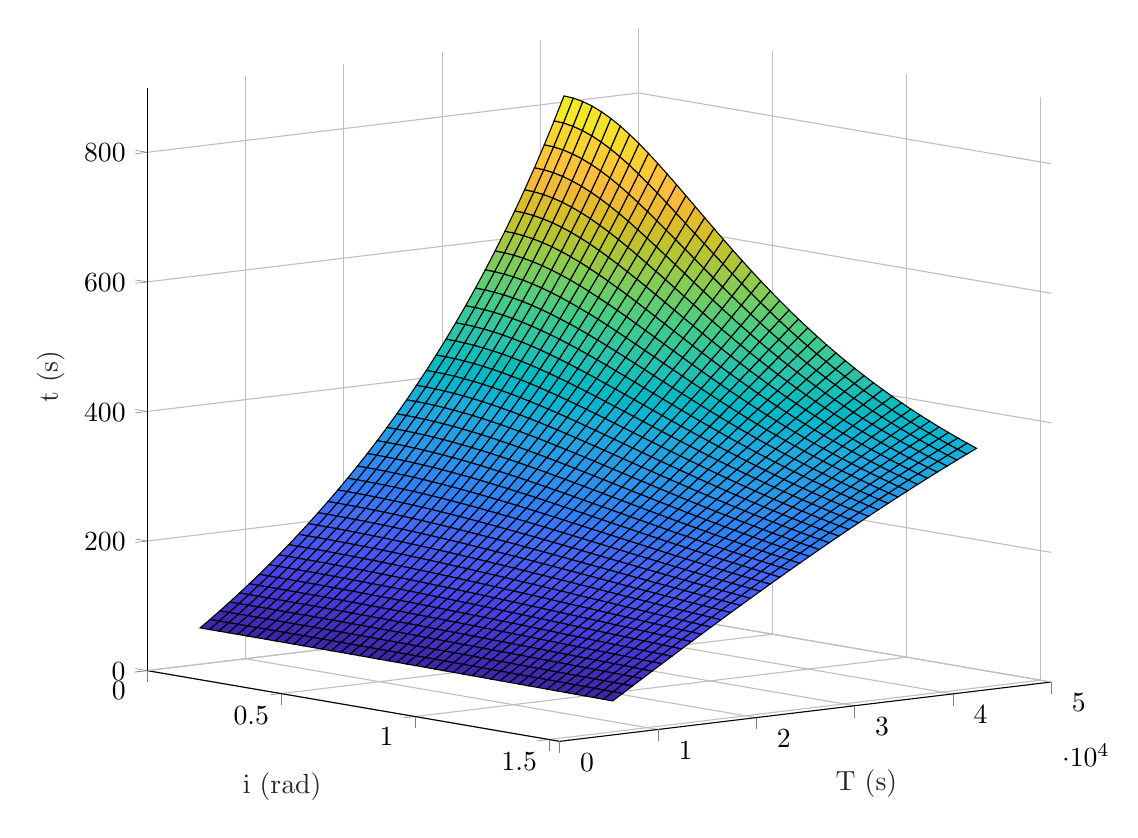
\begin{tikzpicture}

\begin{axis}[%
width=4.521in,
height=3.566in,
at={(0.758in,0.481in)},
scale only axis,
xmin=0,
xmax=1.54,
tick align=outside,
xlabel style={font=\color{white!15!black}},
xlabel={i (rad)},
ymin=0,
ymax=50000,
ylabel style={font=\color{white!15!black}},
ylabel={T (s)},
zmin=0,
zmax=900,
zlabel style={font=\color{white!15!black}},
zlabel={t (s)},
view={-310}{9},
axis background/.style={fill=white},
axis x line*=bottom,
axis y line*=left,
axis z line*=left,
xmajorgrids,
ymajorgrids,
zmajorgrids
]

\addplot3[%
surf,
shader=flat corner, draw=black, z buffer=sort, colormap={mymap}{[1pt] rgb(0pt)=(0.2422,0.1504,0.6603); rgb(1pt)=(0.2444,0.1534,0.6728); rgb(2pt)=(0.2464,0.1569,0.6847); rgb(3pt)=(0.2484,0.1607,0.6961); rgb(4pt)=(0.2503,0.1648,0.7071); rgb(5pt)=(0.2522,0.1689,0.7179); rgb(6pt)=(0.254,0.1732,0.7286); rgb(7pt)=(0.2558,0.1773,0.7393); rgb(8pt)=(0.2576,0.1814,0.7501); rgb(9pt)=(0.2594,0.1854,0.761); rgb(11pt)=(0.2628,0.1932,0.7828); rgb(12pt)=(0.2645,0.1972,0.7937); rgb(13pt)=(0.2661,0.2011,0.8043); rgb(14pt)=(0.2676,0.2052,0.8148); rgb(15pt)=(0.2691,0.2094,0.8249); rgb(16pt)=(0.2704,0.2138,0.8346); rgb(17pt)=(0.2717,0.2184,0.8439); rgb(18pt)=(0.2729,0.2231,0.8528); rgb(19pt)=(0.274,0.228,0.8612); rgb(20pt)=(0.2749,0.233,0.8692); rgb(21pt)=(0.2758,0.2382,0.8767); rgb(22pt)=(0.2766,0.2435,0.884); rgb(23pt)=(0.2774,0.2489,0.8908); rgb(24pt)=(0.2781,0.2543,0.8973); rgb(25pt)=(0.2788,0.2598,0.9035); rgb(26pt)=(0.2794,0.2653,0.9094); rgb(27pt)=(0.2798,0.2708,0.915); rgb(28pt)=(0.2802,0.2764,0.9204); rgb(29pt)=(0.2806,0.2819,0.9255); rgb(30pt)=(0.2809,0.2875,0.9305); rgb(31pt)=(0.2811,0.293,0.9352); rgb(32pt)=(0.2813,0.2985,0.9397); rgb(33pt)=(0.2814,0.304,0.9441); rgb(34pt)=(0.2814,0.3095,0.9483); rgb(35pt)=(0.2813,0.315,0.9524); rgb(36pt)=(0.2811,0.3204,0.9563); rgb(37pt)=(0.2809,0.3259,0.96); rgb(38pt)=(0.2807,0.3313,0.9636); rgb(39pt)=(0.2803,0.3367,0.967); rgb(40pt)=(0.2798,0.3421,0.9702); rgb(41pt)=(0.2791,0.3475,0.9733); rgb(42pt)=(0.2784,0.3529,0.9763); rgb(43pt)=(0.2776,0.3583,0.9791); rgb(44pt)=(0.2766,0.3638,0.9817); rgb(45pt)=(0.2754,0.3693,0.984); rgb(46pt)=(0.2741,0.3748,0.9862); rgb(47pt)=(0.2726,0.3804,0.9881); rgb(48pt)=(0.271,0.386,0.9898); rgb(49pt)=(0.2691,0.3916,0.9912); rgb(50pt)=(0.267,0.3973,0.9924); rgb(51pt)=(0.2647,0.403,0.9935); rgb(52pt)=(0.2621,0.4088,0.9946); rgb(53pt)=(0.2591,0.4145,0.9955); rgb(54pt)=(0.2556,0.4203,0.9965); rgb(55pt)=(0.2517,0.4261,0.9974); rgb(56pt)=(0.2473,0.4319,0.9983); rgb(57pt)=(0.2424,0.4378,0.9991); rgb(58pt)=(0.2369,0.4437,0.9996); rgb(59pt)=(0.2311,0.4497,0.9995); rgb(60pt)=(0.225,0.4559,0.9985); rgb(61pt)=(0.2189,0.462,0.9968); rgb(62pt)=(0.2128,0.4682,0.9948); rgb(63pt)=(0.2066,0.4743,0.9926); rgb(64pt)=(0.2006,0.4803,0.9906); rgb(65pt)=(0.195,0.4861,0.9887); rgb(66pt)=(0.1903,0.4919,0.9867); rgb(67pt)=(0.1869,0.4975,0.9844); rgb(68pt)=(0.1847,0.503,0.9819); rgb(69pt)=(0.1831,0.5084,0.9793); rgb(70pt)=(0.1818,0.5138,0.9766); rgb(71pt)=(0.1806,0.5191,0.9738); rgb(72pt)=(0.1795,0.5244,0.9709); rgb(73pt)=(0.1785,0.5296,0.9677); rgb(74pt)=(0.1778,0.5349,0.9641); rgb(75pt)=(0.1773,0.5401,0.9602); rgb(76pt)=(0.1768,0.5452,0.956); rgb(77pt)=(0.1764,0.5504,0.9516); rgb(78pt)=(0.1755,0.5554,0.9473); rgb(79pt)=(0.174,0.5605,0.9432); rgb(80pt)=(0.1716,0.5655,0.9393); rgb(81pt)=(0.1686,0.5705,0.9357); rgb(82pt)=(0.1649,0.5755,0.9323); rgb(83pt)=(0.161,0.5805,0.9289); rgb(84pt)=(0.1573,0.5854,0.9254); rgb(85pt)=(0.154,0.5902,0.9218); rgb(86pt)=(0.1513,0.595,0.9182); rgb(87pt)=(0.1492,0.5997,0.9147); rgb(88pt)=(0.1475,0.6043,0.9113); rgb(89pt)=(0.1461,0.6089,0.908); rgb(90pt)=(0.1446,0.6135,0.905); rgb(91pt)=(0.1429,0.618,0.9022); rgb(92pt)=(0.1408,0.6226,0.8998); rgb(93pt)=(0.1383,0.6272,0.8975); rgb(94pt)=(0.1354,0.6317,0.8953); rgb(95pt)=(0.1321,0.6363,0.8932); rgb(96pt)=(0.1288,0.6408,0.891); rgb(97pt)=(0.1253,0.6453,0.8887); rgb(98pt)=(0.1219,0.6497,0.8862); rgb(99pt)=(0.1185,0.6541,0.8834); rgb(100pt)=(0.1152,0.6584,0.8804); rgb(101pt)=(0.1119,0.6627,0.877); rgb(102pt)=(0.1085,0.6669,0.8734); rgb(103pt)=(0.1048,0.671,0.8695); rgb(104pt)=(0.1009,0.675,0.8653); rgb(105pt)=(0.0964,0.6789,0.8609); rgb(106pt)=(0.0914,0.6828,0.8562); rgb(107pt)=(0.0855,0.6865,0.8513); rgb(108pt)=(0.0789,0.6902,0.8462); rgb(109pt)=(0.0713,0.6938,0.8409); rgb(110pt)=(0.0628,0.6972,0.8355); rgb(111pt)=(0.0535,0.7006,0.8299); rgb(112pt)=(0.0433,0.7039,0.8242); rgb(113pt)=(0.0328,0.7071,0.8183); rgb(114pt)=(0.0234,0.7103,0.8124); rgb(115pt)=(0.0155,0.7133,0.8064); rgb(116pt)=(0.0091,0.7163,0.8003); rgb(117pt)=(0.0046,0.7192,0.7941); rgb(118pt)=(0.0019,0.722,0.7878); rgb(119pt)=(0.0009,0.7248,0.7815); rgb(120pt)=(0.0018,0.7275,0.7752); rgb(121pt)=(0.0046,0.7301,0.7688); rgb(122pt)=(0.0094,0.7327,0.7623); rgb(123pt)=(0.0162,0.7352,0.7558); rgb(124pt)=(0.0253,0.7376,0.7492); rgb(125pt)=(0.0369,0.74,0.7426); rgb(126pt)=(0.0504,0.7423,0.7359); rgb(127pt)=(0.0638,0.7446,0.7292); rgb(128pt)=(0.077,0.7468,0.7224); rgb(129pt)=(0.0899,0.7489,0.7156); rgb(130pt)=(0.1023,0.751,0.7088); rgb(131pt)=(0.1141,0.7531,0.7019); rgb(132pt)=(0.1252,0.7552,0.695); rgb(133pt)=(0.1354,0.7572,0.6881); rgb(134pt)=(0.1448,0.7593,0.6812); rgb(135pt)=(0.1532,0.7614,0.6741); rgb(136pt)=(0.1609,0.7635,0.6671); rgb(137pt)=(0.1678,0.7656,0.6599); rgb(138pt)=(0.1741,0.7678,0.6527); rgb(139pt)=(0.1799,0.7699,0.6454); rgb(140pt)=(0.1853,0.7721,0.6379); rgb(141pt)=(0.1905,0.7743,0.6303); rgb(142pt)=(0.1954,0.7765,0.6225); rgb(143pt)=(0.2003,0.7787,0.6146); rgb(144pt)=(0.2061,0.7808,0.6065); rgb(145pt)=(0.2118,0.7828,0.5983); rgb(146pt)=(0.2178,0.7849,0.5899); rgb(147pt)=(0.2244,0.7869,0.5813); rgb(148pt)=(0.2318,0.7887,0.5725); rgb(149pt)=(0.2401,0.7905,0.5636); rgb(150pt)=(0.2491,0.7922,0.5546); rgb(151pt)=(0.2589,0.7937,0.5454); rgb(152pt)=(0.2695,0.7951,0.536); rgb(153pt)=(0.2809,0.7964,0.5266); rgb(154pt)=(0.2929,0.7975,0.517); rgb(155pt)=(0.3052,0.7985,0.5074); rgb(156pt)=(0.3176,0.7994,0.4975); rgb(157pt)=(0.3301,0.8002,0.4876); rgb(158pt)=(0.3424,0.8009,0.4774); rgb(159pt)=(0.3548,0.8016,0.4669); rgb(160pt)=(0.3671,0.8021,0.4563); rgb(161pt)=(0.3795,0.8026,0.4454); rgb(162pt)=(0.3921,0.8029,0.4344); rgb(163pt)=(0.405,0.8031,0.4233); rgb(164pt)=(0.4184,0.803,0.4122); rgb(165pt)=(0.4322,0.8028,0.4013); rgb(166pt)=(0.4463,0.8024,0.3904); rgb(167pt)=(0.4608,0.8018,0.3797); rgb(168pt)=(0.4753,0.8011,0.3691); rgb(169pt)=(0.4899,0.8002,0.3586); rgb(170pt)=(0.5044,0.7993,0.348); rgb(171pt)=(0.5187,0.7982,0.3374); rgb(172pt)=(0.5329,0.797,0.3267); rgb(173pt)=(0.547,0.7957,0.3159); rgb(175pt)=(0.5748,0.7929,0.2941); rgb(176pt)=(0.5886,0.7913,0.2833); rgb(177pt)=(0.6024,0.7896,0.2726); rgb(178pt)=(0.6161,0.7878,0.2622); rgb(179pt)=(0.6297,0.7859,0.2521); rgb(180pt)=(0.6433,0.7839,0.2423); rgb(181pt)=(0.6567,0.7818,0.2329); rgb(182pt)=(0.6701,0.7796,0.2239); rgb(183pt)=(0.6833,0.7773,0.2155); rgb(184pt)=(0.6963,0.775,0.2075); rgb(185pt)=(0.7091,0.7727,0.1998); rgb(186pt)=(0.7218,0.7703,0.1924); rgb(187pt)=(0.7344,0.7679,0.1852); rgb(188pt)=(0.7468,0.7654,0.1782); rgb(189pt)=(0.759,0.7629,0.1717); rgb(190pt)=(0.771,0.7604,0.1658); rgb(191pt)=(0.7829,0.7579,0.1608); rgb(192pt)=(0.7945,0.7554,0.157); rgb(193pt)=(0.806,0.7529,0.1546); rgb(194pt)=(0.8172,0.7505,0.1535); rgb(195pt)=(0.8281,0.7481,0.1536); rgb(196pt)=(0.8389,0.7457,0.1546); rgb(197pt)=(0.8495,0.7435,0.1564); rgb(198pt)=(0.86,0.7413,0.1587); rgb(199pt)=(0.8703,0.7392,0.1615); rgb(200pt)=(0.8804,0.7372,0.165); rgb(201pt)=(0.8903,0.7353,0.1695); rgb(202pt)=(0.9,0.7336,0.1749); rgb(203pt)=(0.9093,0.7321,0.1815); rgb(204pt)=(0.9184,0.7308,0.189); rgb(205pt)=(0.9272,0.7298,0.1973); rgb(206pt)=(0.9357,0.729,0.2061); rgb(207pt)=(0.944,0.7285,0.2151); rgb(208pt)=(0.9523,0.7284,0.2237); rgb(209pt)=(0.9606,0.7285,0.2312); rgb(210pt)=(0.9689,0.7292,0.2373); rgb(211pt)=(0.977,0.7304,0.2418); rgb(212pt)=(0.9842,0.733,0.2446); rgb(213pt)=(0.99,0.7365,0.2429); rgb(214pt)=(0.9946,0.7407,0.2394); rgb(215pt)=(0.9966,0.7458,0.2351); rgb(216pt)=(0.9971,0.7513,0.2309); rgb(217pt)=(0.9972,0.7569,0.2267); rgb(218pt)=(0.9971,0.7626,0.2224); rgb(219pt)=(0.9969,0.7683,0.2181); rgb(220pt)=(0.9966,0.774,0.2138); rgb(221pt)=(0.9962,0.7798,0.2095); rgb(222pt)=(0.9957,0.7856,0.2053); rgb(223pt)=(0.9949,0.7915,0.2012); rgb(224pt)=(0.9938,0.7974,0.1974); rgb(225pt)=(0.9923,0.8034,0.1939); rgb(226pt)=(0.9906,0.8095,0.1906); rgb(227pt)=(0.9885,0.8156,0.1875); rgb(228pt)=(0.9861,0.8218,0.1846); rgb(229pt)=(0.9835,0.828,0.1817); rgb(230pt)=(0.9807,0.8342,0.1787); rgb(231pt)=(0.9778,0.8404,0.1757); rgb(232pt)=(0.9748,0.8467,0.1726); rgb(233pt)=(0.972,0.8529,0.1695); rgb(234pt)=(0.9694,0.8591,0.1665); rgb(235pt)=(0.9671,0.8654,0.1636); rgb(236pt)=(0.9651,0.8716,0.1608); rgb(237pt)=(0.9634,0.8778,0.1582); rgb(238pt)=(0.9619,0.884,0.1557); rgb(239pt)=(0.9608,0.8902,0.1532); rgb(240pt)=(0.9601,0.8963,0.1507); rgb(241pt)=(0.9596,0.9023,0.148); rgb(242pt)=(0.9595,0.9084,0.145); rgb(243pt)=(0.9597,0.9143,0.1418); rgb(244pt)=(0.9601,0.9203,0.1382); rgb(245pt)=(0.9608,0.9262,0.1344); rgb(246pt)=(0.9618,0.932,0.1304); rgb(247pt)=(0.9629,0.9379,0.1261); rgb(248pt)=(0.9642,0.9437,0.1216); rgb(249pt)=(0.9657,0.9494,0.1168); rgb(250pt)=(0.9674,0.9552,0.1116); rgb(251pt)=(0.9692,0.9609,0.1061); rgb(252pt)=(0.9711,0.9667,0.1001); rgb(253pt)=(0.973,0.9724,0.0938); rgb(254pt)=(0.9749,0.9782,0.0872); rgb(255pt)=(0.9769,0.9839,0.0805)}, mesh/rows=45]
table[row sep=crcr, point meta=\thisrow{c}] {%
%
x	y	z	c\\
0	5400	56	56\\
0	6400	67.2	67.2\\
0	7400	78.6835443037975	78.6835443037975\\
0	8400	90.4615384615385	90.4615384615385\\
0	9400	102.545454545455	102.545454545455\\
0	10400	114.947368421053	114.947368421053\\
0	11400	127.68	127.68\\
0	12400	140.756756756757	140.756756756757\\
0	13400	154.191780821918	154.191780821918\\
0	14400	168	168\\
0	15400	182.197183098592	182.197183098592\\
0	16400	196.8	196.8\\
0	17400	211.826086956522	211.826086956522\\
0	18400	227.294117647059	227.294117647059\\
0	19400	243.223880597015	243.223880597015\\
0	20400	259.636363636364	259.636363636364\\
0	21400	276.553846153846	276.553846153846\\
0	22400	294	294\\
0	23400	312	312\\
0	24400	330.58064516129	330.58064516129\\
0	25400	349.770491803279	349.770491803279\\
0	26400	369.6	369.6\\
0	27400	390.101694915254	390.101694915254\\
0	28400	411.310344827586	411.310344827586\\
0	29400	433.263157894737	433.263157894737\\
0	30400	456	456\\
0	31400	479.563636363636	479.563636363636\\
0	32400	504	504\\
0	33400	529.358490566038	529.358490566038\\
0	34400	555.692307692308	555.692307692308\\
0	35400	583.058823529412	583.058823529412\\
0	36400	611.52	611.52\\
0	37400	641.142857142857	641.142857142857\\
0	38400	672	672\\
0	39400	704.170212765958	704.170212765958\\
0	40400	737.739130434783	737.739130434783\\
0	41400	772.8	772.8\\
0	42400	809.454545454546	809.454545454546\\
0.035	5400	55.9975612971825	55.9975612971825\\
0.035	6400	67.1964444212269	67.1964444212269\\
0.035	7400	78.6786080658929	78.6786080658929\\
0.035	8400	90.4549302800604	90.4549302800604\\
0.035	9400	102.536852857731	102.536852857731\\
0.035	10400	114.93641830738	114.93641830738\\
0.035	11400	127.666309766816	127.666309766816\\
0.035	12400	140.739894140764	140.739894140764\\
0.035	13400	154.171268768654	154.171268768654\\
0.035	14400	167.97531196397	167.97531196397\\
0.035	15400	182.167737804823	182.167737804823\\
0.035	16400	196.765155598438	196.765155598438\\
0.035	17400	211.785134490994	211.785134490994\\
0.035	18400	227.24627374928	227.24627374928\\
0.035	19400	243.168279303091	243.168279303091\\
0.035	20400	259.572047208099	259.572047208099\\
0.035	21400	276.479754769559	276.479754769559\\
0.035	22400	293.914960158995	293.914960158995\\
0.035	23400	311.902711460816	311.902711460816\\
0.035	24400	330.469666205732	330.469666205732\\
0.035	25400	349.64422258516	349.64422258516\\
0.035	26400	369.456663698677	369.456663698677\\
0.035	27400	389.939316368122	389.939316368122\\
0.035	28400	411.126726261444	411.126726261444\\
0.035	29400	433.055851311588	433.055851311588\\
0.035	30400	455.766275696301	455.766275696301\\
0.035	31400	479.300446970774	479.300446970774\\
0.035	32400	503.703939324655	503.703939324655\\
0.035	33400	529.025746378203	529.025746378203\\
0.035	34400	555.318607451279	555.318607451279\\
0.035	35400	582.639371848002	582.639371848002\\
0.035	36400	611.049406417077	611.049406417077\\
0.035	37400	640.615052494642	640.615052494642\\
0.035	38400	671.408139339471	671.408139339471\\
0.035	39400	703.50656236223	703.50656236223\\
0.035	40400	736.994935871291	736.994935871291\\
0.035	41400	771.965331757367	771.965331757367\\
0.035	42400	808.518117579786	808.518117579786\\
0.07	5400	55.9902500856498	55.9902500856498\\
0.07	6400	67.1857854229613	67.1857854229613\\
0.07	7400	78.6638109667858	78.6638109667858\\
0.07	8400	90.4351225092879	90.4351225092879\\
0.07	9400	102.511071302908	102.511071302908\\
0.07	10400	114.903600132277	114.903600132277\\
0.07	11400	127.62528222447	127.62528222447\\
0.07	12400	140.689363260666	140.689363260666\\
0.07	13400	154.109806780432	154.109806780432\\
0.07	14400	167.901343301379	167.901343301379\\
0.07	15400	182.079523512399	182.079523512399\\
0.07	16400	196.6607759385	196.6607759385\\
0.07	17400	211.662469520195	211.662469520195\\
0.07	18400	227.102981600988	227.102981600988\\
0.07	19400	243.001771873729	243.001771873729\\
0.07	20400	259.379462901368	259.379462901368\\
0.07	21400	276.257927900991	276.257927900991\\
0.07	22400	293.660386563375	293.660386563375\\
0.07	23400	311.611509775064	311.611509775064\\
0.07	24400	330.13753421795	330.13753421795\\
0.07	25400	349.266387944626	349.266387944626\\
0.07	26400	369.027828168733	369.027828168733\\
0.07	27400	389.453592671063	389.453592671063\\
0.07	28400	410.577566407613	410.577566407613\\
0.07	29400	432.435965119123	432.435965119123\\
0.07	30400	455.067537987527	455.067537987527\\
0.07	31400	478.51379166887	478.51379166887\\
0.07	32400	502.819238361074	502.819238361074\\
0.07	33400	528.031670946632	528.031670946632\\
0.07	34400	554.202468694044	554.202468694044\\
0.07	35400	581.386937519266	581.386937519266\\
0.07	36400	609.644689412965	609.644689412965\\
0.07	37400	639.040066347644	639.040066347644\\
0.07	38400	669.642614810532	669.642614810532\\
0.07	39400	701.527618087564	701.527618087564\\
0.07	40400	734.776694580318	734.776694580318\\
0.07	41400	769.478471806897	769.478471806897\\
0.07	42400	805.729347363441	805.729347363441\\
0.105	5400	55.978081036663	55.978081036663\\
0.105	6400	67.1680461843939	67.1680461843939\\
0.105	7400	78.6391877913849	78.6391877913849\\
0.105	8400	90.402165375552	90.402165375552\\
0.105	9400	102.468180259482	102.468180259482\\
0.105	10400	114.849010173229	114.849010173229\\
0.105	11400	127.557046521536	127.557046521536\\
0.105	12400	140.605334555809	140.605334555809\\
0.105	13400	154.007616716012	154.007616716012\\
0.105	14400	167.778379435435	167.778379435435\\
0.105	15400	181.932903732259	181.932903732259\\
0.105	16400	196.487319946619	196.487319946619\\
0.105	17400	211.458667020737	211.458667020737\\
0.105	18400	226.864956763402	226.864956763402\\
0.105	19400	242.725243589115	242.725243589115\\
0.105	20400	259.059700277442	259.059700277442\\
0.105	21400	275.8897003603	275.8897003603\\
0.105	22400	293.237907815076	293.237907815076\\
0.105	23400	311.128374820741	311.128374820741\\
0.105	24400	329.586648423768	329.586648423768\\
0.105	25400	348.639887062281	348.639887062281\\
0.105	26400	368.31698801207	368.31698801207\\
0.105	27400	388.648726949036	388.648726949036\\
0.105	28400	409.667910971607	409.667910971607\\
0.105	29400	431.409546596356	431.409546596356\\
0.105	30400	453.911024433757	453.911024433757\\
0.105	31400	477.212322472291	477.212322472291\\
0.105	32400	501.356230152414	501.356230152414\\
0.105	33400	526.388595702141	526.388595702141\\
0.105	34400	552.358599539165	552.358599539165\\
0.105	35400	579.319056927311	579.319056927311\\
0.105	36400	607.32675351579	607.32675351579\\
0.105	37400	636.442817897573	636.442817897573\\
0.105	38400	666.733135909187	666.733135909187\\
0.105	39400	698.26881207119	698.26881207119\\
0.105	40400	731.126684351446	731.126684351446\\
0.105	41400	765.38989933953	765.38989933953\\
0.105	42400	801.148555970364	801.148555970364\\
0.14	5400	55.9610785374807	55.9610785374807\\
0.14	6400	67.1432652212536	67.1432652212536\\
0.14	7400	78.6047963187556	78.6047963187556\\
0.14	8400	90.3561422749416	90.3561422749416\\
0.14	9400	102.408296538235	102.408296538235\\
0.14	10400	114.772808161498	114.772808161498\\
0.14	11400	127.461816833561	127.461816833561\\
0.14	12400	140.488090551553	140.488090551553\\
0.14	13400	153.865066164841	153.865066164841\\
0.14	14400	167.606893044258	167.606893044258\\
0.14	15400	181.728480155603	181.728480155603\\
0.14	16400	196.245546844568	196.245546844568\\
0.14	17400	211.174677671484	211.174677671484\\
0.14	18400	226.533381669108	226.533381669108\\
0.14	19400	242.340156435364	242.340156435364\\
0.14	20400	258.614557516123	258.614557516123\\
0.14	21400	275.377273581188	275.377273581188\\
0.14	22400	292.650207950336	292.650207950336\\
0.14	23400	310.456567086161	310.456567086161\\
0.14	24400	328.820956737413	328.820956737413\\
0.14	25400	347.769486491317	347.769486491317\\
0.14	26400	367.329883577031	367.329883577031\\
0.14	27400	387.531616855953	387.531616855953\\
0.14	28400	408.406032039352	408.406032039352\\
0.14	29400	429.986499290957	429.986499290957\\
0.14	30400	452.308574503359	452.308574503359\\
0.14	31400	475.41017568386	475.41017568386\\
0.14	32400	499.33177604962	499.33177604962\\
0.14	33400	524.116615615569	524.116615615569\\
0.14	34400	549.810933263572	549.810933263572\\
0.14	35400	576.464221510101	576.464221510101\\
0.14	36400	604.129506444303	604.129506444303\\
0.14	37400	632.863655591267	632.863655591267\\
0.14	38400	662.727716768475	662.727716768475\\
0.14	39400	693.787291348845	693.787291348845\\
0.14	40400	726.112945722563	726.112945722563\\
0.14	41400	759.780665162457	759.780665162457\\
0.14	42400	794.872354742718	794.872354742718\\
0.175	5400	55.9392765946292	55.9392765946292\\
0.175	6400	67.1114962125119	67.1114962125119\\
0.175	7400	78.5607170304984	78.5607170304984\\
0.175	8400	90.2971693052713	90.2971693052713\\
0.175	9400	102.331582658423	102.331582658423\\
0.175	10400	114.675216195595	114.675216195595\\
0.175	11400	127.339890771425	127.339890771425\\
0.175	12400	140.338023574689	140.338023574689\\
0.175	13400	153.682665223722	153.682665223722\\
0.175	14400	167.387539579316	167.387539579316\\
0.175	15400	181.467086501166	181.467086501166\\
0.175	16400	195.936507794495	195.936507794495\\
0.175	17400	210.811816616121	210.811816616121\\
0.175	18400	226.109890633938	226.109890633938\\
0.175	19400	241.848529260918	241.848529260918\\
0.175	20400	258.046515314365	258.046515314365\\
0.175	21400	274.723681483632	274.723681483632\\
0.175	22400	291.90098202493	291.90098202493\\
0.175	23400	309.6005701406	309.6005701406\\
0.175	24400	327.845881542345	327.845881542345\\
0.175	25400	346.66172474387	346.66172474387\\
0.175	26400	366.074378678136	366.074378678136\\
0.175	27400	386.111698288377	386.111698288377\\
0.175	28400	406.803228800178	406.803228800178\\
0.175	29400	428.18032944434	428.18032944434\\
0.175	30400	450.276307466969	450.276307466969\\
0.175	31400	473.126563333927	473.126563333927\\
0.175	32400	496.768748111155	496.768748111155\\
0.175	33400	521.242934079586	521.242934079586\\
0.175	34400	546.591799722454	546.591799722454\\
0.175	35400	572.860830301919	572.860830301919\\
0.175	36400	600.0985353189	600.0985353189\\
0.175	37400	628.356684221351	628.356684221351\\
0.175	38400	657.690561787405	657.690561787405\\
0.175	39400	688.159244654548	688.159244654548\\
0.175	40400	719.825900485765	719.825900485765\\
0.175	41400	752.758111247094	752.758111247094\\
0.175	42400	787.028222002904	787.028222002904\\
0.21	5400	55.9127186995428	55.9127186995428\\
0.21	6400	67.0728077599265	67.0728077599265\\
0.21	7400	78.5070527065501	78.5070527065501\\
0.21	8400	90.2253946180906	90.2253946180906\\
0.21	9400	102.238245846803	102.238245846803\\
0.21	10400	114.556517240507	114.556517240507\\
0.21	11400	127.191647185601	127.191647185601\\
0.21	12400	140.155632605815	140.155632605815\\
0.21	13400	153.461062061811	153.461062061811\\
0.21	14400	167.121151107901	167.121151107901\\
0.21	15400	181.149780074066	181.149780074066\\
0.21	16400	195.561534454195	195.561534454195\\
0.21	17400	210.371748095012	210.371748095012\\
0.21	18400	225.596549394508	225.596549394508\\
0.21	19400	241.252910733879	241.252910733879\\
0.21	20400	257.358701382909	257.358701382909\\
0.21	21400	273.932744135347	273.932744135347\\
0.21	22400	290.994875948102	290.994875948102\\
0.21	23400	308.566012875714	308.566012875714\\
0.21	24400	326.668219609468	326.668219609468\\
0.21	25400	345.324783948328	345.324783948328\\
0.21	26400	364.560296546173	364.560296546173\\
0.21	27400	384.400736296072	384.400736296072\\
0.21	28400	404.873561726888	404.873561726888\\
0.21	29400	426.007808799284	426.007808799284\\
0.21	30400	447.834195496167	447.834195496167\\
0.21	31400	470.385233605069	470.385233605069\\
0.21	32400	493.695348085042	493.695348085042\\
0.21	33400	517.801004395743	517.801004395743\\
0.21	34400	542.740844138308	542.740844138308\\
0.21	35400	568.555829312377	568.555829312377\\
0.21	36400	595.289395425935	595.289395425935\\
0.21	37400	622.987613598217	622.987613598217\\
0.21	38400	651.69936166248	651.69936166248\\
0.21	39400	681.476504094854	681.476504094854\\
0.21	40400	712.374080354973	712.374080354973\\
0.21	41400	744.450500907594	744.450500907594\\
0.21	42400	777.767749782096	777.767749782096\\
0.245	5400	55.8814576576189	55.8814576576189\\
0.245	6400	67.0272830825455	67.0272830825455\\
0.245	7400	78.4439279123955	78.4439279123955\\
0.245	8400	90.140997597831	90.140997597831\\
0.245	9400	102.128536771585	102.128536771585\\
0.245	10400	114.417053232492	114.417053232492\\
0.245	11400	127.017543397931	127.017543397931\\
0.245	12400	139.941519317881	139.941519317881\\
0.245	13400	153.201037348964	153.201037348964\\
0.245	14400	166.80872859204	166.80872859204\\
0.245	15400	180.777831202085	180.777831202085\\
0.245	16400	195.122224684163	195.122224684163\\
0.245	17400	209.856466294097	209.856466294097\\
0.245	18400	224.995829666928	224.995829666928\\
0.245	19400	240.556345800111	240.556345800111\\
0.245	20400	256.554846521534	256.554846521534\\
0.245	21400	273.009010574413	273.009010574413\\
0.245	22400	289.937412451758	289.937412451758\\
0.245	23400	307.359574111775	307.359574111775\\
0.245	24400	325.296019701859	325.296019701859\\
0.245	25400	343.768333412033	343.768333412033\\
0.245	26400	362.799220567944	362.799220567944\\
0.245	27400	382.412572057867	382.412572057867\\
0.245	28400	402.633532166335	402.633532166335\\
0.245	29400	423.488569857517	423.488569857517\\
0.245	30400	445.005553512414	445.005553512414\\
0.245	31400	467.213829073194	467.213829073194\\
0.245	32400	490.144301482674	490.144301482674\\
0.245	33400	513.82951922394	513.82951922394\\
0.245	34400	538.303761660226	538.303761660226\\
0.245	35400	563.603128743681	563.603128743681\\
0.245	36400	589.765632497729	589.765632497729\\
0.245	37400	616.831289474208	616.831289474208\\
0.245	38400	644.84221313509	644.84221313509\\
0.245	39400	673.842704799033	673.842704799033\\
0.245	40400	703.879341413388	703.879341413388\\
0.245	41400	735.001057948113	735.001057948113\\
0.245	42400	767.259221642454	767.259221642454\\
0.28	5400	55.8455553820094	55.8455553820094\\
0.28	6400	66.9750196488442	66.9750196488442\\
0.28	7400	78.3714883827108	78.3714883827108\\
0.28	8400	90.0441878769939	90.0441878769939\\
0.28	9400	102.002748026407	102.002748026407\\
0.28	10400	114.257222814203	114.257222814203\\
0.28	11400	126.818111900253	126.818111900253\\
0.28	12400	139.696383361968	139.696383361968\\
0.28	13400	152.903497640263	152.903497640263\\
0.28	14400	166.45143274249	166.45143274249\\
0.28	15400	180.352710753276	180.352710753276\\
0.28	16400	194.62042570231	194.62042570231\\
0.28	17400	209.268272835192	209.268272835192\\
0.28	18400	224.310579329156	224.310579329156\\
0.28	19400	239.762336489595	239.762336489595\\
0.28	20400	255.639233455408	255.639233455408\\
0.28	21400	271.957692430912	271.957692430912\\
0.28	22400	288.734905448842	288.734905448842\\
0.28	23400	305.988872652301	305.988872652301\\
0.28	24400	323.738442062529	323.738442062529\\
0.28	25400	342.003350773419	342.003350773419\\
0.28	26400	360.804267481633	360.804267481633\\
0.28	27400	380.162836221817	380.162836221817\\
0.28	28400	400.101721128474	400.101721128474\\
0.28	29400	420.644651987735	420.644651987735\\
0.28	30400	441.816470271693	441.816470271693\\
0.28	31400	463.643175262884	463.643175262884\\
0.28	32400	486.1519697741	486.1519697741\\
0.28	33400	509.371304846035	509.371304846035\\
0.28	34400	533.330922658482	533.330922658482\\
0.28	35400	558.061896715804	558.061896715804\\
0.28	36400	583.596668159249	583.596668159249\\
0.28	37400	609.969076811732	609.969076811732\\
0.28	38400	637.214385268634	637.214385268634\\
0.28	39400	665.369294003648	665.369294003648\\
0.28	40400	694.471945053656	694.471945053656\\
0.28	41400	724.561911372129	724.561911372129\\
0.28	42400	755.680168386739	755.680168386739\\
0.315	5400	55.8050826537284	55.8050826537284\\
0.315	6400	66.9161287496827	66.9161287496827\\
0.315	7400	78.2899003074018	78.2899003074018\\
0.315	8400	89.93520419793	89.93520419793\\
0.315	9400	101.861212382194	101.861212382194\\
0.315	10400	114.077478729252	114.077478729252\\
0.315	11400	126.593956566066	126.593956566066\\
0.315	12400	139.421016971696	139.421016971696\\
0.315	13400	152.569467824839	152.569467824839\\
0.315	14400	166.050573608629	166.050573608629\\
0.315	15400	179.876075970423	179.876075970423\\
0.315	16400	194.058215026661	194.058215026661\\
0.315	17400	208.609751393592	208.609751393592\\
0.315	18400	223.543988913392	223.543988913392\\
0.315	19400	238.874798031601	238.874798031601\\
0.315	20400	254.616639765468	254.616639765468\\
0.315	21400	270.784590183321	270.784590183321\\
0.315	22400	287.394365291804	287.394365291804\\
0.315	23400	304.462346200218	304.462346200218\\
0.315	24400	322.005604398538	322.005604398538\\
0.315	25400	340.041926947028	340.041926947028\\
0.315	26400	358.589841329905	358.589841329905\\
0.315	27400	377.668639672002	377.668639672002\\
0.315	28400	397.298401954657	397.298401954657\\
0.315	29400	417.500017793645	417.500017793645\\
0.315	30400	438.295206256242	438.295206256242\\
0.315	31400	459.706533094635	459.706533094635\\
0.315	32400	481.757424656848	481.757424656848\\
0.315	33400	504.472177601739	504.472177601739\\
0.315	34400	527.875963389036	527.875963389036\\
0.315	35400	551.994826335983	551.994826335983\\
0.315	36400	576.85567382597	576.85567382597\\
0.315	37400	602.486257018444	602.486257018444\\
0.315	38400	628.915140140119	628.915140140119\\
0.315	39400	656.17165613186	656.17165613186\\
0.315	40400	684.28584608041	684.28584608041\\
0.315	41400	713.288379476866	713.288379476866\\
0.315	42400	743.210451912264	743.210451912264\\
0.35	5400	55.7601188498946	55.7601188498946\\
0.35	6400	66.8507350157404	66.8507350157404\\
0.35	7400	78.1993495268593	78.1993495268593\\
0.35	8400	89.8143131332262	89.8143131332262\\
0.35	9400	101.704300827126	101.704300827126\\
0.35	10400	113.878324909144	113.878324909144\\
0.35	11400	126.345748427172	126.345748427172\\
0.35	12400	139.116298966225	139.116298966225\\
0.35	13400	152.200082759535	152.200082759535\\
0.35	14400	165.607599082678	165.607599082678\\
0.35	15400	179.349754882381	179.349754882381\\
0.35	16400	193.437879579704	193.437879579704\\
0.35	17400	207.883739973449	207.883739973449\\
0.35	18400	222.699555153451	222.699555153451\\
0.35	19400	237.898011314624	237.898011314624\\
0.35	20400	253.49227634083	253.49227634083\\
0.35	21400	269.496014002416	269.496014002416\\
0.35	22400	285.923397582117	285.923397582117\\
0.35	23400	302.789122710379	302.789122710379\\
0.35	24400	320.108419152537	320.108419152537\\
0.35	25400	337.897061245776	337.897061245776\\
0.35	26400	356.171376632915	356.171376632915\\
0.35	27400	374.948252881784	374.948252881784\\
0.35	28400	394.245141512456	394.245141512456\\
0.35	29400	414.080058878939	414.080058878939\\
0.35	30400	434.471583265942	434.471583265942\\
0.35	31400	455.438847464106	455.438847464106\\
0.35	32400	477.001525977286	477.001525977286\\
0.35	33400	499.17981589211	499.17981589211\\
0.35	34400	521.994410301925	521.994410301925\\
0.35	35400	545.466463023378	545.466463023378\\
0.35	36400	569.617543173447	569.617543173447\\
0.35	37400	594.469577987087	594.469577987087\\
0.35	38400	620.044782050722	620.044782050722\\
0.35	39400	646.365570904996	646.365570904996\\
0.35	40400	673.454456732643	673.454456732643\\
0.35	41400	701.333923596643	701.333923596643\\
0.35	42400	730.026279433484	730.026279433484\\
0.385	5400	55.7107516421428	55.7107516421428\\
0.385	6400	66.7789758835011	66.7789758835011\\
0.385	7400	78.1000406439963	78.1000406439963\\
0.385	8400	89.6818076779747	89.6818076779747\\
0.385	9400	101.532420417015	101.532420417015\\
0.385	10400	113.660313288598	113.660313288598\\
0.385	11400	126.074221071854	126.074221071854\\
0.385	12400	138.78318823849	138.78318823849\\
0.385	13400	151.796578217288	151.796578217288\\
0.385	14400	165.124082509424	165.124082509424\\
0.385	15400	178.775729569134	178.775729569134\\
0.385	16400	192.761893349728	192.761893349728\\
0.385	17400	207.093301398385	207.093301398385\\
0.385	18400	221.781042364354	221.781042364354\\
0.385	19400	236.836572763766	236.836572763766\\
0.385	20400	252.271722820034	252.271722820034\\
0.385	21400	268.098701171396	268.098701171396\\
0.385	22400	284.330098206144	284.330098206144\\
0.385	23400	300.978887751204	300.978887751204\\
0.385	24400	318.05842680046	318.05842680046\\
0.385	25400	335.582452925223	335.582452925223\\
0.385	26400	353.565078959994	353.565078959994\\
0.385	27400	372.020784501819	372.020784501819\\
0.385	28400	390.9644037005	390.9644037005\\
0.385	29400	410.411108749466	410.411108749466\\
0.385	30400	430.376388412676	430.376388412676\\
0.385	31400	450.87602084132	450.87602084132\\
0.385	32400	471.92603984514	471.92603984514\\
0.385	33400	493.542693686795	493.542693686795\\
0.385	34400	515.742395364158	515.742395364158\\
0.385	35400	538.541663235176	538.541663235176\\
0.385	36400	561.957050723915	561.957050723915\\
0.385	37400	586.005063726039	586.005063726039\\
0.385	38400	610.702064209321	610.702064209321\\
0.385	39400	636.064158382711	636.064158382711\\
0.385	40400	662.107067689952	662.107067689952\\
0.385	41400	688.845980775778	688.845980775778\\
0.385	42400	716.295384481017	716.295384481017\\
0.42	5400	55.6570766674334	55.6570766674334\\
0.42	6400	66.7010010142282	66.7010010142282\\
0.42	7400	77.9921960612686	77.9921960612686\\
0.42	8400	89.5380057282349	89.5380057282349\\
0.42	9400	101.346011959939	101.346011959939\\
0.42	10400	113.424040387674	113.424040387674\\
0.42	11400	125.780165724592	125.780165724592\\
0.42	12400	138.422716819974	138.422716819974\\
0.42	13400	151.360281286248	151.360281286248\\
0.42	14400	164.601709600275	164.601709600275\\
0.42	15400	178.156118566537	178.156118566537\\
0.42	16400	192.032894014398	192.032894014398\\
0.42	17400	206.241692584224	206.241692584224\\
0.42	18400	220.792442437875	220.792442437875\\
0.42	19400	235.695342707517	235.695342707517\\
0.42	20400	250.960861472858	250.960861472858\\
0.42	21400	266.599732030457	266.599732030457\\
0.42	22400	282.622947189539	282.622947189539\\
0.42	23400	299.041751296605	299.041751296605\\
0.42	24400	315.867629655866	315.867629655866\\
0.42	25400	333.112294973984	333.112294973984\\
0.42	26400	350.787670415684	350.787670415684\\
0.42	27400	368.905868811456	368.905868811456\\
0.42	28400	387.479167509739	387.479167509739\\
0.42	29400	406.519978313869	406.519978313869\\
0.42	30400	426.040811888784	426.040811888784\\
0.42	31400	446.054235964527	446.054235964527\\
0.42	32400	466.572826603419	466.572826603419\\
0.42	33400	487.609111736324	487.609111736324\\
0.42	34400	509.175506111805	509.175506111805\\
0.42	35400	531.284236741616	531.284236741616\\
0.42	36400	553.947257869032	553.947257869032\\
0.42	37400	577.176154435284	577.176154435284\\
0.42	38400	600.982032977137	600.982032977137\\
0.42	39400	625.375398859226	625.375398859226\\
0.42	40400	650.366018732858	650.366018732858\\
0.42	41400	675.962767124248	675.962767124248\\
0.42	42400	702.173456096224	702.173456096224\\
0.455	5400	55.5991971736494	55.5991971736494\\
0.455	6400	66.6169716706676	66.6169716706676\\
0.455	7400	77.8760549513894	77.8760549513894\\
0.455	8400	89.3832484608036	89.3832484608036\\
0.455	9400	101.145547560218	101.145547560218\\
0.455	10400	113.170143700789	113.170143700789\\
0.455	11400	125.464426069458	125.464426069458\\
0.455	12400	138.03598261598	138.03598261598\\
0.455	13400	150.892600358554	150.892600358554\\
0.455	14400	164.042264853165	164.042264853165\\
0.455	15400	177.493158698125	177.493158698125\\
0.455	16400	191.253658930342	191.253658930342\\
0.455	17400	205.332333153449	205.332333153449\\
0.455	18400	219.737934220005	219.737934220005\\
0.455	19400	234.479393270477	234.479393270477\\
0.455	20400	249.565810910566	249.565810910566\\
0.455	21400	265.006446285546	265.006446285546\\
0.455	22400	280.810703785724	280.810703785724\\
0.455	23400	296.988117090779	296.988117090779\\
0.455	24400	313.548330232792	313.548330232792\\
0.455	25400	330.501075328193	330.501075328193\\
0.455	26400	347.85614659794	347.85614659794\\
0.455	27400	365.623370263158	365.623370263158\\
0.455	28400	383.812569870623	383.812569870623\\
0.455	29400	402.433526569353	402.433526569353\\
0.455	30400	421.4959338268	421.4959338268\\
0.455	31400	441.009346041586	441.009346041586\\
0.455	32400	460.983120480359	460.983120480359\\
0.455	33400	481.426351940584	481.426351940584\\
0.455	34400	502.347799520362	502.347799520362\\
0.455	35400	523.755804862753	523.755804862753\\
0.455	36400	545.658201237756	545.658201237756\\
0.455	37400	568.062212832806	568.062212832806\\
0.455	38400	590.974343645563	590.974343645563\\
0.455	39400	614.400255414407	614.400255414407\\
0.455	40400	638.344634086653	638.344634086653\\
0.455	41400	662.811044416459	662.811044416459\\
0.455	42400	687.801772408814	687.801772408814\\
0.49	5400	55.5372236425111	55.5372236425111\\
0.49	6400	66.5270600564618	66.5270600564618\\
0.49	7400	77.7518721708328	77.7518721708328\\
0.49	8400	89.217898629974	89.217898629974\\
0.49	9400	100.93152804755	100.93152804755\\
0.49	10400	112.899297933611	112.899297933611\\
0.49	11400	125.127892880297	125.127892880297\\
0.49	12400	137.624141906021	137.624141906021\\
0.49	13400	150.395014847511	150.395014847511\\
0.49	14400	163.447617677772	163.447617677772\\
0.49	15400	176.789186615774	176.789186615774\\
0.49	16400	190.427080880572	190.427080880572\\
0.49	17400	204.368773928476	204.368773928476\\
0.49	18400	218.621842996938	218.621842996938\\
0.49	19400	233.193956762927	233.193956762927\\
0.49	20400	248.092860906905	248.092860906905\\
0.49	21400	263.32636135601	263.32636135601\\
0.49	22400	278.902304961994	278.902304961994\\
0.49	23400	294.828557350916	294.828557350916\\
0.49	24400	311.112977662761	311.112977662761\\
0.49	25400	327.76338988048	327.76338988048\\
0.49	26400	344.787550429611	344.787550429611\\
0.49	27400	362.19311171227	362.19311171227\\
0.49	28400	379.987581223384	379.987581223384\\
0.49	29400	398.178275883325	398.178275883325\\
0.49	30400	416.772271210421	416.772271210421\\
0.49	31400	435.776344950176	435.776344950176\\
0.49	32400	455.196914776615	455.196914776615\\
0.49	33400	475.039969686387	475.039969686387\\
0.49	34400	495.310994719624	495.310994719624\\
0.49	35400	516.014888664951	516.014888664951\\
0.49	36400	537.155874441429	537.155874441429\\
0.49	37400	558.73740189987	558.73740189987\\
0.49	38400	580.762042852288	580.762042852288\\
0.49	39400	603.231378223827	603.231378223827\\
0.49	40400	626.145877329123	626.145877329123\\
0.49	41400	649.504769407304	649.504769407304\\
0.49	42400	673.305907709565	673.305907709565\\
0.525	5400	55.4712733924448	55.4712733924448\\
0.525	6400	66.431448623432	66.431448623432\\
0.525	7400	77.6199171254827	77.6199171254827\\
0.525	8400	89.0423387972879	89.0423387972879\\
0.525	9400	100.704480317479	100.704480317479\\
0.525	10400	112.612211129023	112.612211129023\\
0.525	11400	124.771498520554	124.771498520554\\
0.525	12400	137.188401702739	137.188401702739\\
0.525	13400	149.869064768812	149.869064768812\\
0.525	14400	162.819708419028	162.819708419028\\
0.525	15400	176.046620318833	176.046620318833\\
0.525	16400	189.556143950242	189.556143950242\\
0.525	17400	203.354665805176	203.354665805176\\
0.525	18400	217.448600758553	217.448600758553\\
0.525	19400	231.844375447705	231.844375447705\\
0.525	20400	246.54840947353	246.54840947353\\
0.525	21400	261.567094227719	261.567094227719\\
0.525	22400	276.906769139699	276.906769139699\\
0.525	23400	292.573695126954	292.573695126954\\
0.525	24400	308.574025023285	308.574025023285\\
0.525	25400	324.913770751979	324.913770751979\\
0.525	26400	341.598767005017	341.598767005017\\
0.525	27400	358.634631186105	358.634631186105\\
0.525	28400	376.026719375018	376.026719375018\\
0.525	29400	393.780078074206	393.780078074206\\
0.525	30400	411.89939150682	411.89939150682\\
0.525	31400	430.388924249052	430.388924249052\\
0.525	32400	449.252459000111	449.252459000111\\
0.525	33400	468.49322932144	468.49322932144\\
0.525	34400	488.113847214117	488.113847214117\\
0.525	35400	508.116225451173	508.116225451173\\
0.525	36400	528.501494641175	528.501494641175\\
0.525	37400	549.269915072297	549.269915072297\\
0.525	38400	570.420783473641	570.420783473641\\
0.525	39400	591.952334934036	591.952334934036\\
0.525	40400	613.861640339227	613.861640339227\\
0.525	41400	636.144499827005	636.144499827005\\
0.525	42400	658.795332917114	658.795332917114\\
0.56	5400	55.4014701641222	55.4014701641222\\
0.56	6400	66.3303293520014	66.3303293520014\\
0.56	7400	77.480472597909	77.480472597909\\
0.56	8400	88.8569695103824	88.8569695103824\\
0.56	9400	100.464954609271	100.464954609271\\
0.56	10400	112.309620722863	112.309620722863\\
0.56	11400	124.396211374259	124.396211374259\\
0.56	12400	136.730012059822	136.730012059822\\
0.56	13400	149.316340315705	149.316340315705\\
0.56	14400	162.160534461579	162.160534461579\\
0.56	15400	175.267940903644	175.267940903644\\
0.56	16400	188.64389987213	188.64389987213\\
0.56	17400	202.293729461651	202.293729461651\\
0.56	18400	216.222707836336	216.222707836336\\
0.56	19400	230.436053455611	230.436053455611\\
0.56	20400	244.93890317114	244.93890317114\\
0.56	21400	259.736288040998	259.736288040998\\
0.56	22400	274.833106703843	274.833106703843\\
0.56	23400	290.234096154095	290.234096154095\\
0.56	24400	305.943799759206	305.943799759206\\
0.56	25400	321.966532362492	321.966532362492\\
0.56	26400	338.306342320152	338.306342320152\\
0.56	27400	354.96697032952	354.96697032952\\
0.56	28400	371.951804917947	371.951804917947\\
0.56	29400	389.263834478522	389.263834478522\\
0.56	30400	406.905595760927	406.905595760927\\
0.56	31400	424.879118753687	424.879118753687\\
0.56	32400	443.18586792879	443.18586792879\\
0.56	33400	461.82667986185	461.82667986185\\
0.56	34400	480.801697291394	480.801697291394\\
0.56	35400	500.110299740331	500.110299740331\\
0.56	36400	519.751030891734	519.751030891734\\
0.56	37400	539.721522990418	539.721522990418\\
0.56	38400	560.018418631724	560.018418631724\\
0.56	39400	580.637290399678	580.637290399678\\
0.56	40400	601.572558928102	601.572558928102\\
0.56	41400	622.817410079826	622.817410079826\\
0.56	42400	644.363712070023	644.363712070023\\
0.595	5400	55.3279436914329	55.3279436914329\\
0.595	6400	66.2239030100841	66.2239030100841\\
0.595	7400	77.3338335457692	77.3338335457692\\
0.595	8400	88.6622074468946	88.6622074468946\\
0.595	9400	100.213521746822	100.213521746822\\
0.595	10400	111.992289568994	111.992289568994\\
0.595	11400	124.003030267306	124.003030267306\\
0.595	12400	136.250258414871	136.250258414871\\
0.595	13400	148.738471550007	148.738471550007\\
0.595	14400	161.472136584208	161.472136584208\\
0.595	15400	174.45567477307	174.45567477307\\
0.595	16400	187.693445147857	187.693445147857\\
0.595	17400	201.189726302684	201.189726302684\\
0.595	18400	214.94869643034	214.94869643034\\
0.595	19400	228.974411498825	228.974411498825\\
0.595	20400	243.270781460851	243.270781460851\\
0.595	21400	257.841544390222	257.841544390222\\
0.595	22400	272.690238442321	272.690238442321\\
0.595	23400	287.820171541329	287.820171541329\\
0.595	24400	303.234388704494	303.234388704494\\
0.595	25400	318.93563692421	318.93563692421\\
0.595	26400	334.926327542257	334.926327542257\\
0.595	27400	351.208496067622	351.208496067622\\
0.595	28400	367.783759410417	367.783759410417\\
0.595	29400	384.65327052992	384.65327052992\\
0.595	30400	401.817670525107	401.817670525107\\
0.595	31400	419.277038231748	419.277038231748\\
0.595	32400	437.030837431477	437.030837431477\\
0.595	33400	455.077861825673	455.077861825673\\
0.595	34400	473.416177980732	473.416177980732\\
0.595	35400	492.04306651149	492.04306651149\\
0.595	36400	510.954961836276	510.954961836276\\
0.595	37400	530.147390910132	530.147390910132\\
0.595	38400	549.614911421754	549.614911421754\\
0.595	39400	569.351050024039	569.351050024039\\
0.595	40400	589.348241256923	589.348241256923\\
0.595	41400	609.597767913007	609.597767913007\\
0.595	42400	630.089703689802	630.089703689802\\
0.63	5400	55.250829260679	55.250829260679\\
0.63	6400	66.1123783957523	66.1123783957523\\
0.63	7400	77.180305880719	77.180305880719\\
0.63	8400	88.4584835390529	88.4584835390529\\
0.63	9400	99.9507703674093	99.9507703674093\\
0.63	10400	111.661001971573	111.661001971573\\
0.63	11400	123.592978934926	123.592978934926\\
0.63	12400	135.75045404737	135.75045404737\\
0.63	13400	148.137118320914	148.137118320914\\
0.63	14400	160.756585716974	160.756585716974\\
0.63	15400	173.612376509847	173.612376509847\\
0.63	16400	186.707899211035	186.707899211035\\
0.63	17400	200.046430980264	200.046430980264\\
0.63	18400	213.631096451229	213.631096451229\\
0.63	19400	227.464844903628	227.464844903628\\
0.63	20400	241.55042571805	241.55042571805\\
0.63	21400	255.890362056972	255.890362056972\\
0.63	22400	270.486922723758	270.486922723758\\
0.63	23400	285.342092162413	285.342092162413\\
0.63	24400	300.457538574116	300.457538574116\\
0.63	25400	315.834580142578	315.834580142578\\
0.63	26400	331.474149379274	331.474149379274\\
0.63	27400	347.376755621851	347.376755621851\\
0.63	28400	363.542445744754	363.542445744754\\
0.63	29400	379.970763170586	379.970763170586\\
0.63	30400	396.660705304076	396.660705304076\\
0.63	31400	413.610679547905	413.610679547905\\
0.63	32400	430.818458101124	430.818458101124\\
0.63	33400	448.28113178638	448.28113178638\\
0.63	34400	465.995063201604	465.995063201604\\
0.63	35400	483.955839544808	483.955839544808\\
0.63	36400	502.158225516873	502.158225516873\\
0.63	37400	520.596116765965	520.596116765965\\
0.63	38400	539.26249439772	539.26249439772\\
0.63	39400	558.149381136541	558.149381136541\\
0.63	40400	577.247799783981	577.247799783981\\
0.63	41400	596.547734678612	596.547734678612\\
0.63	42400	616.038096916426	616.038096916426\\
0.665	5400	55.1702672607664	55.1702672607664\\
0.665	6400	65.9959715689296	65.9959715689296\\
0.665	7400	77.0202052370027	77.0202052370027\\
0.665	8400	88.2462410940419	88.2462410940419\\
0.665	9400	99.6773041619485	99.6773041619485\\
0.665	10400	111.31655976017	111.31655976017\\
0.665	11400	123.167100587234	123.167100587234\\
0.665	12400	135.231932724985	135.231932724985\\
0.665	13400	147.513960512173	147.513960512173\\
0.665	14400	160.015970235597	160.015970235597\\
0.665	15400	172.740612589327	172.740612589327\\
0.665	16400	185.690383855877	185.690383855877\\
0.665	17400	198.867605767619	198.867605767619\\
0.665	18400	212.274404012438	212.274404012438\\
0.665	19400	225.912685354674	225.912685354674\\
0.665	20400	239.784113351112	239.784113351112\\
0.665	21400	253.890082652133	253.890082652133\\
0.665	22400	268.23169189048	268.23169189048\\
0.665	23400	282.809715174421	282.809715174421\\
0.665	24400	297.624572218715	297.624572218715\\
0.665	25400	312.67629716572	312.67629716572\\
0.665	26400	327.964506170439	327.964506170439\\
0.665	27400	343.488363847321	343.488363847321\\
0.665	28400	359.24654870329	359.24654870329\\
0.665	29400	375.237217710798	375.237217710798\\
0.665	30400	391.457970206578	391.457970206578\\
0.665	31400	407.905811336165	407.905811336165\\
0.665	32400	424.577115300851	424.577115300851\\
0.665	33400	441.467588702342	441.467588702342\\
0.665	34400	458.572234320491	458.572234320491\\
0.665	35400	475.885315700539	475.885315700539\\
0.665	36400	493.400322967763	493.400322967763\\
0.665	37400	511.109940328259	511.109940328259\\
0.665	38400	529.006015754039	529.006015754039\\
0.665	39400	547.079533387417	547.079533387417\\
0.665	40400	565.320589232633	565.320589232633\\
0.665	41400	583.718370730362	583.718370730362\\
0.665	42400	602.261140831763	602.261140831763\\
0.7	5400	55.0864027271391	55.0864027271391\\
0.7	6400	65.8749050772344	65.8749050772344\\
0.7	7400	76.8538557385715	76.8538557385715\\
0.7	8400	88.0259339245259	88.0259339245259\\
0.7	9400	99.3937391489992	99.3937391489992\\
0.7	10400	110.95977844075	110.95977844075\\
0.7	11400	122.726452620113	122.726452620113\\
0.7	12400	134.696041603697	134.696041603697\\
0.7	13400	146.870688705677	146.870688705677\\
0.7	14400	159.252383908123	159.252383908123\\
0.7	15400	171.84294607759	171.84294607759\\
0.7	16400	184.644004110995	184.644004110995\\
0.7	17400	197.656977000782	197.656977000782\\
0.7	18400	210.88305281756	210.88305281756\\
0.7	19400	224.323166617974	224.323166617974\\
0.7	20400	237.977977296602	237.977977296602\\
0.7	21400	251.847843413226	251.847843413226\\
0.7	22400	265.932798041078	265.932798041078\\
0.7	23400	280.232522697545	280.232522697545\\
0.7	24400	294.746320436547	294.746320436547\\
0.7	25400	309.473088201199	309.473088201199\\
0.7	26400	324.411288556638	324.411288556638\\
0.7	27400	339.558920945767	339.558920945767\\
0.7	28400	354.913492635237	354.913492635237\\
0.7	29400	370.471989544925	370.471989544925\\
0.7	30400	386.230847181387	386.230847181387\\
0.7	31400	402.185921923892	402.185921923892\\
0.7	32400	418.332462940343	418.332462940343\\
0.7	33400	434.665085039177	434.665085039177\\
0.7	34400	451.177742791735	451.177742791735\\
0.7	35400	467.863706286882	467.863706286882\\
0.7	36400	484.715538905164	484.715538905164\\
0.7	37400	501.72507752272	501.72507752272\\
0.7	38400	518.883415574589	518.883415574589\\
0.7	39400	536.180889422035	536.180889422035\\
0.7	40400	553.607068478086	553.607068478086\\
0.7	41400	571.150749548553	571.150749548553\\
0.7	42400	588.799955841404	588.799955841404\\
0.735	5400	54.9993848821405	54.9993848821405\\
0.735	6400	65.7494071809266	65.7494071809266\\
0.735	7400	76.6815887731746	76.6815887731746\\
0.735	8400	87.7980245028566	87.7980245028566\\
0.735	9400	99.1007010031309	99.1007010031309\\
0.735	10400	110.591483452577	110.591483452577\\
0.735	11400	122.272101513618	122.272101513618\\
0.735	12400	134.144134438932	134.144134438932\\
0.735	13400	146.208995336396	146.208995336396\\
0.735	14400	158.467914588782	158.467914588782\\
0.735	15400	170.921922430911	170.921922430911\\
0.735	16400	183.571830694547	183.571830694547\\
0.735	17400	196.418213739879	196.418213739879\\
0.735	18400	209.461388602121	209.461388602121\\
0.735	19400	222.701394392641	222.701394392641\\
0.735	20400	236.137971006066	236.137971006066\\
0.735	21400	249.770537198096	249.770537198096\\
0.735	22400	263.598168113229	263.598168113229\\
0.735	23400	277.619572357339	277.619572357339\\
0.735	24400	291.833068726859	291.833068726859\\
0.735	25400	306.236562724252	306.236562724252\\
0.735	26400	320.827523008319	320.827523008319\\
0.735	27400	335.602957947558	335.602957947558\\
0.735	28400	350.559392465004	350.559392465004\\
0.735	29400	365.692845383529	365.692845383529\\
0.735	30400	380.998807501182	380.998807501182\\
0.735	31400	396.472220646279	396.472220646279\\
0.735	32400	412.107457981415	412.107457981415\\
0.735	33400	427.898305843648	427.898305843648\\
0.735	34400	443.837947424471	443.837947424471\\
0.735	35400	459.918948607042	459.918948607042\\
0.735	36400	476.133246289071	476.133246289071\\
0.735	37400	492.472139526951	492.472139526951\\
0.735	38400	508.92628383956	508.92628383956\\
0.735	39400	525.485689007973	525.485689007973\\
0.735	40400	542.13972069949	542.13972069949\\
0.735	41400	558.877106230229	558.877106230229\\
0.735	42400	575.68594475962	575.68594475962\\
0.77	5400	54.9093666744045	54.9093666744045\\
0.77	6400	65.619711081695	65.619711081695\\
0.77	7400	76.5037417813773	76.5037417813773\\
0.77	8400	87.5629821515091	87.5629821515091\\
0.77	9400	98.7988224564063	98.7988224564063\\
0.77	10400	110.212506557842	110.212506557842\\
0.77	11400	121.805117954687	121.805117954687\\
0.77	12400	133.577565156198	133.577565156198\\
0.77	13400	145.530566400142	145.530566400142\\
0.77	14400	157.66463373376	157.66463373376\\
0.77	15400	169.980056483127	169.980056483127\\
0.77	16400	182.476884144913	182.476884144913\\
0.77	17400	195.154908743837	195.154908743837\\
0.77	18400	208.013646709249	208.013646709249\\
0.77	19400	221.052320335301	221.052320335301\\
0.77	20400	234.269838901015	234.269838901015\\
0.77	21400	247.664779539203	247.664779539203\\
0.77	22400	261.235367956579	261.235367956579\\
0.77	23400	274.979459121386	274.979459121386\\
0.77	24400	288.894518049442	288.894518049442\\
0.77	25400	302.977600834339	302.977600834339\\
0.77	26400	317.225336082638	317.225336082638\\
0.77	27400	331.633906929925	331.633906929925\\
0.77	28400	346.199033828269	346.199033828269\\
0.77	29400	360.915958309801	360.915958309801\\
0.77	30400	375.779427944261	375.779427944261\\
0.77	31400	390.783682720241	390.783682720241\\
0.77	32400	405.922443090061	405.922443090061\\
0.77	33400	421.188899926191	421.188899926191\\
0.77	34400	436.575706642646	436.575706642646\\
0.77	35400	452.074973737184	452.074973737184\\
0.77	36400	467.678266009101	467.678266009101\\
0.77	37400	483.376602702419	483.376602702419\\
0.77	38400	499.160460814999	499.160460814999\\
0.77	39400	515.019781800039	515.019781800039\\
0.77	40400	530.943981867493	530.943981867493\\
0.77	41400	546.921966068653	546.921966068653\\
0.77	42400	562.942146317635	562.942146317635\\
0.805	5400	54.8165043197758	54.8165043197758\\
0.805	6400	65.4860541597653	65.4860541597653\\
0.805	7400	76.320657067912	76.320657067912\\
0.805	8400	87.3212812812062	87.3212812812062\\
0.805	9400	98.488740789774	98.488740789774\\
0.805	10400	109.823682387471	109.823682387471\\
0.805	11400	121.326572215382	121.326572215382\\
0.805	12400	132.997681820979	132.997681820979\\
0.805	13400	144.837073762317	144.837073762317\\
0.805	14400	156.844586793959	156.844586793959\\
0.805	15400	169.019820679189	169.019820679189\\
0.805	16400	181.362120681624	181.362120681624\\
0.805	17400	193.870561798449	193.870561798449\\
0.805	18400	206.543932807171	206.543932807171\\
0.805	19400	219.38072020799	219.38072020799\\
0.805	20400	232.379092154507	232.379092154507\\
0.805	21400	245.536882476429	245.536882476429\\
0.805	22400	258.851574909168	258.851574909168\\
0.805	23400	272.320287656495	272.320287656495\\
0.805	24400	285.939758423613	285.939758423613\\
0.805	25400	299.706330069019	299.706330069019\\
0.805	26400	313.615937033979	313.615937033979\\
0.805	27400	327.664092718245	327.664092718245\\
0.805	28400	341.845877979477	341.845877979477\\
0.805	29400	356.155930941392	356.155930941392\\
0.805	30400	370.58843830171	370.58843830171\\
0.805	31400	385.137128335158	385.137128335158\\
0.805	32400	399.795265788791	399.795265788791\\
0.805	33400	414.55564886643	414.55564886643\\
0.805	34400	429.41060849576	429.41060849576\\
0.805	35400	444.352010065291	444.352010065291\\
0.805	36400	459.371257808709	459.371257808709\\
0.805	37400	474.459302000941	474.459302000941\\
0.805	38400	489.606649113297	489.606649113297\\
0.805	39400	504.803375054338	504.803375054338\\
0.805	40400	520.039141598497	520.039141598497\\
0.805	41400	535.303216076192	535.303216076192\\
0.805	42400	550.584494367142	550.584494367142\\
0.84	5400	54.7209568461367	54.7209568461367\\
0.84	6400	65.3486772235226	65.3486772235226\\
0.84	7400	76.1326806421568	76.1326806421568\\
0.84	8400	87.0733996870315	87.0733996870315\\
0.84	9400	98.1710954290944	98.1710954290944\\
0.84	10400	109.425845163018	109.425845163018\\
0.84	11400	120.837529812253	120.837529812253\\
0.84	12400	132.405821038926	132.405821038926\\
0.84	13400	144.130168102847	144.130168102847\\
0.84	14400	156.009784521058	156.009784521058\\
0.84	15400	168.043634586867	168.043634586867\\
0.84	16400	180.230419815257	180.230419815257\\
0.84	17400	192.568565389731	192.568565389731\\
0.84	18400	205.05620669413	205.05620669413\\
0.84	19400	217.691176021515	217.691176021515\\
0.84	20400	230.47098956086	230.47098956086\\
0.84	21400	243.392834770824	243.392834770824\\
0.84	22400	256.45355825824	256.45355825824\\
0.84	23400	269.649654286878	269.649654286878\\
0.84	24400	282.977254049503	282.977254049503\\
0.84	25400	296.432115842909	296.432115842909\\
0.84	26400	310.009616291363	310.009616291363\\
0.84	27400	323.704742768538	323.704742768538\\
0.84	28400	337.512087171213	337.512087171213\\
0.84	29400	351.425841199685	351.425841199685\\
0.84	30400	365.439793299695	365.439793299695\\
0.84	31400	379.547327418408	379.547327418408\\
0.84	32400	393.7414237226	393.7414237226\\
0.84	33400	408.01466142028	408.01466142028\\
0.84	34400	422.35922381756	422.35922381756\\
0.84	35400	436.766905730378	436.766905730378\\
0.84	36400	451.229123355746	451.229123355746\\
0.84	37400	465.736926689422	465.736926689422\\
0.84	38400	480.281014556356	480.281014556356\\
0.84	39400	494.851752296991	494.851752296991\\
0.84	40400	509.439192126786	509.439192126786\\
0.84	41400	524.033096158231	524.033096158231\\
0.84	42400	538.622962044654	538.622962044654\\
0.875	5400	54.6228856443802	54.6228856443802\\
0.875	6400	65.2078237755199	65.2078237755199\\
0.875	7400	75.9401610938954	75.9401610938954\\
0.875	8400	86.8198169116218	86.8198169116218\\
0.875	9400	97.8465256584015	97.8465256584015\\
0.875	10400	109.019825611107	109.019825611107\\
0.875	11400	120.339047466918	120.339047466918\\
0.875	12400	131.803302809033	131.803302809033\\
0.875	13400	143.411472520194	143.411472520194\\
0.875	14400	155.162195205748	155.162195205748\\
0.875	15400	167.053855694573	167.053855694573\\
0.875	16400	179.084573692906	179.084573692906\\
0.875	17400	191.252192672822	191.252192672822\\
0.875	18400	203.554269083781	203.554269083781\\
0.875	19400	215.988061982085	215.988061982085\\
0.875	20400	228.550523179264	228.550523179264\\
0.875	21400	241.238288016151	241.238288016151\\
0.875	22400	254.04766687454	254.04766687454\\
0.875	23400	266.974637542814	266.974637542814\\
0.875	24400	280.014838555465	280.014838555465\\
0.875	25400	293.163563629014	293.163563629014\\
0.875	26400	306.415757318157	306.415757318157\\
0.875	27400	319.766012015952	319.766012015952\\
0.875	28400	333.208566420347	333.208566420347\\
0.875	29400	346.737305586099	346.737305586099\\
0.875	30400	360.345762676142	360.345762676142\\
0.875	31400	374.0271225195	374.0271225195\\
0.875	32400	387.774227073895	387.774227073895\\
0.875	33400	401.579582880096	401.579582880096\\
0.875	34400	415.435370581975	415.435370581975\\
0.875	35400	429.333456570894	429.333456570894\\
0.875	36400	443.265406795818	443.265406795818\\
0.875	37400	457.222502761278	457.222502761278\\
0.875	38400	471.195759714324	471.195759714324\\
0.875	39400	485.175946999042	485.175946999042\\
0.875	40400	499.153610533346	499.153610533346\\
0.875	41400	513.119097337899	513.119097337899\\
0.875	42400	527.062582021579	527.062582021579\\
0.91	5400	54.5224540276174	54.5224540276174\\
0.91	6400	65.0637392984119	65.0637392984119\\
0.91	7400	75.7434485098299	75.7434485098299\\
0.91	8400	86.5610126832883	86.5610126832883\\
0.91	9400	97.515668460881	97.515668460881\\
0.91	10400	108.606448083383	108.606448083383\\
0.91	11400	119.832169382557	119.832169382557\\
0.91	12400	131.191425844474	131.191425844474\\
0.91	13400	142.682576805904	142.682576805904\\
0.91	14400	154.303737851144	154.303737851144\\
0.91	15400	166.052771481923	166.052771481923\\
0.91	16400	177.927278138094	177.927278138094\\
0.91	17400	189.92458765171	189.92458765171\\
0.91	18400	202.041751221549	202.041751221549\\
0.91	19400	214.275533999247	214.275533999247\\
0.91	20400	226.622408381677	226.622408381677\\
0.91	21400	239.078548107057	239.078548107057\\
0.91	22400	251.639823254278	251.639823254278\\
0.91	23400	264.301796246051	264.301796246051\\
0.91	24400	277.059718956543	277.059718956543\\
0.91	25400	289.908531023054	289.908531023054\\
0.91	26400	302.842859458904	302.842859458904\\
0.91	27400	315.857019660962	315.857019660962\\
0.91	28400	328.945017899988	328.945017899988\\
0.91	29400	342.100555375214	342.100555375214\\
0.91	30400	355.317033906245	355.317033906245\\
0.91	31400	368.587563325347	368.587563325347\\
0.91	32400	381.904970621668	381.904970621668\\
0.91	33400	395.261810875738	395.261810875738\\
0.91	34400	408.650380007958	408.650380007958\\
0.91	35400	422.062729348748	422.062729348748\\
0.91	36400	435.490682020688	435.490682020688\\
0.91	37400	448.925851104664	448.925851104664\\
0.91	38400	462.359659542783	462.359659542783\\
0.91	39400	475.783361711052	475.783361711052\\
0.91	40400	489.188066574699	489.188066574699\\
0.91	41400	502.564762318954	502.564762318954\\
0.91	42400	515.904342328378	515.904342328378\\
0.945	5400	54.4198268005428	54.4198268005428\\
0.945	6400	64.9166705639933	64.9166705639933\\
0.945	7400	75.5428934356303	75.5428934356303\\
0.945	8400	86.297465435673	86.297465435673\\
0.945	9400	97.1791564959463	97.1791564959463\\
0.945	10400	108.186527891638	108.186527891638\\
0.945	11400	119.317923845977	119.317923845977\\
0.945	12400	130.571463368386	130.571463368386\\
0.945	13400	141.945032390738	141.945032390738\\
0.945	14400	153.436276270262	153.436276270262\\
0.945	15400	165.042592731206	165.042592731206\\
0.945	16400	176.761125320668	176.761125320668\\
0.945	17400	188.588757456762	188.588757456762\\
0.945	18400	200.522107149573	200.522107149573\\
0.945	19400	212.557522476995	212.557522476995\\
0.945	20400	224.691077898432	224.691077898432\\
0.945	21400	236.918571489471	236.918571489471\\
0.945	22400	249.2355231798	249.2355231798\\
0.945	23400	261.637174074821	261.637174074821\\
0.945	24400	274.118486938583	274.118486938583\\
0.945	25400	286.67414791157	286.67414791157\\
0.945	26400	299.298569531702	299.298569531702\\
0.945	27400	311.985895120451	311.985895120451\\
0.945	28400	324.730004588247	324.730004588247\\
0.945	29400	337.524521704375	337.524521704375\\
0.945	30400	350.362822866379	350.362822866379\\
0.945	31400	363.238047392571	363.238047392571\\
0.945	32400	376.143109348752	376.143109348752\\
0.945	33400	389.070710906719	389.070710906719\\
0.945	34400	402.013357217763	402.013357217763\\
0.945	35400	414.96337276923	414.96337276923\\
0.945	36400	427.912919176582	427.912919176582\\
0.945	37400	440.854014347444	440.854014347444\\
0.945	38400	453.778552938045	453.778552938045\\
0.945	39400	466.678328006605	466.678328006605\\
0.945	40400	479.545053752726	479.545053752726\\
0.945	41400	492.370389217098	492.370389217098\\
0.945	42400	505.145962802024	505.145962802024\\
0.98	5400	54.315169840713	54.315169840713\\
0.98	6400	64.7668649681576	64.7668649681576\\
0.98	7400	75.3388458876025	75.3388458876025\\
0.98	8400	86.0296509143104	86.0296509143104\\
0.98	9400	96.837616218761	96.837616218761\\
0.98	10400	107.760868864549	107.760868864549\\
0.98	11400	118.797320160145	118.797320160145\\
0.98	12400	129.944659385127	129.944659385127\\
0.98	13400	141.200347954154	141.200347954154\\
0.98	14400	152.561614084191	152.561614084191\\
0.98	15400	164.025448032396	164.025448032396\\
0.98	16400	175.58859797336	175.58859797336\\
0.98	17400	187.247566585202	187.247566585202\\
0.98	18400	198.998608414098	198.998608414098\\
0.98	19400	210.837728086222	210.837728086222\\
0.98	20400	222.760679434673	222.760679434673\\
0.98	21400	234.762965606705	234.762965606705\\
0.98	22400	246.839840213416	246.839840213416\\
0.98	23400	258.986309579965	258.986309579965\\
0.98	24400	271.197136149262	271.197136149262\\
0.98	25400	283.466843086036	283.466843086036\\
0.98	26400	295.789720121052	295.789720121052\\
0.98	27400	308.159830667226	308.159830667226\\
0.98	28400	320.571020230298	320.571020230298\\
0.98	29400	333.016926126863	333.016926126863\\
0.98	30400	345.490988511754	345.490988511754\\
0.98	31400	357.986462705338	357.986462705338\\
0.98	32400	370.496432799155	370.496432799155\\
0.98	33400	383.01382650583	383.01382650583\\
0.98	34400	395.531431206246	395.531431206246\\
0.98	35400	408.041911134022	408.041911134022\\
0.98	36400	420.537825624327	420.537825624327\\
0.98	37400	433.011648341368	433.011648341368\\
0.98	38400	445.455787386642	445.455787386642\\
0.98	39400	457.862606178426	457.862606178426\\
0.98	40400	470.224444982279	470.224444982279\\
0.98	41400	482.533642962695	482.533642962695\\
0.98	42400	494.78256061766	494.78256061766\\
1.015	5400	54.2086496933137	54.2086496933137\\
1.015	6400	64.6145698942253	64.6145698942253\\
1.015	7400	75.1316544173642	75.1316544173642\\
1.015	8400	85.7580408742698	85.7580408742698\\
1.015	9400	96.4916661466099	96.4916661466099\\
1.015	10400	107.33026112953	107.33026112953\\
1.015	11400	118.271345907725	118.271345907725\\
1.015	12400	129.312225421448	129.312225421448\\
1.015	13400	140.449985680806	140.449985680806\\
1.015	14400	151.681490587309	151.681490587309\\
1.015	15400	163.003379421766	163.003379421766\\
1.015	16400	174.412065057152	174.412065057152\\
1.015	17400	185.903732953964	185.903732953964\\
1.015	18400	197.474340993754	197.474340993754\\
1.015	19400	209.119620204053	209.119620204053\\
1.015	20400	220.835076424557	220.835076424557\\
1.015	21400	232.6159929604	232.6159929604\\
1.015	22400	244.457434263421	244.457434263421\\
1.015	23400	256.354250676651	256.354250676651\\
1.015	24400	268.301084270736	268.301084270736\\
1.015	25400	280.292375793724	280.292375793724\\
1.015	26400	292.322372747651	292.322372747651\\
1.015	27400	304.385138596631	304.385138596631\\
1.015	28400	316.474563101893	316.474563101893\\
1.015	29400	328.584373769337	328.584373769337\\
1.015	30400	340.708148384977	340.708148384977\\
1.015	31400	352.839328603085	352.839328603085\\
1.015	32400	364.971234541165	364.971234541165\\
1.015	33400	377.097080325162	377.097080325162\\
1.015	34400	389.209990517754	389.209990517754\\
1.015	35400	401.303017352289	401.303017352289\\
1.015	36400	413.369158685126	413.369158685126\\
1.015	37400	425.40137656996	425.40137656996\\
1.015	38400	437.392616349314	437.392616349314\\
1.015	39400	449.335826150973	449.335826150973\\
1.015	40400	461.223976670727	461.223976670727\\
1.015	41400	473.050081117708	473.050081117708\\
1.015	42400	484.807215194769	484.807215194769\\
1.05	5400	54.1004331808112	54.1004331808112\\
1.05	6400	64.4600321067154	64.4600321067154\\
1.05	7400	74.9216652322392	74.9216652322392\\
1.05	8400	85.4831018718942	85.4831018718942\\
1.05	9400	96.1419152746917	96.1419152746917\\
1.05	10400	106.895479120426	106.895479120426\\
1.05	11400	117.740964542301	117.740964542301\\
1.05	12400	128.67533772675	128.67533772675\\
1.05	13400	139.695358140917	139.695358140917\\
1.05	14400	150.797577437394	150.797577437394\\
1.05	15400	161.978339084328	161.978339084328\\
1.05	16400	173.233778766974	173.233778766974\\
1.05	17400	184.559825604072	184.559825604072\\
1.05	18400	195.952204219091	195.952204219091\\
1.05	19400	207.406437702402	207.406437702402\\
1.05	20400	218.917851495753	218.917851495753\\
1.05	21400	230.481578225108	230.481578225108\\
1.05	22400	242.092563501941	242.092563501941\\
1.05	23400	253.745572706497	253.745572706497\\
1.05	24400	265.435198759373	265.435198759373\\
1.05	25400	277.155870880115	277.155870880115\\
1.05	26400	288.901864323414	288.901864323414\\
1.05	27400	300.667311074994	300.667311074994\\
1.05	28400	312.446211480577	312.446211480577\\
1.05	29400	324.232446772332	324.232446772332\\
1.05	30400	336.01979244832	336.01979244832\\
1.05	31400	347.801932451489	347.801932451489\\
1.05	32400	359.572474086116	359.572474086116\\
1.05	33400	371.324963601184	371.324963601184\\
1.05	34400	383.052902362297	383.052902362297\\
1.05	35400	394.749763526406	394.749763526406\\
1.05	36400	406.409009127007	406.409009127007\\
1.05	37400	418.024107471716	418.024107471716\\
1.05	38400	429.588550749302	429.588550749302\\
1.05	39400	441.095872739468	441.095872739468\\
1.05	40400	452.539666516022	452.539666516022\\
1.05	41400	463.913602032583	463.913602032583\\
1.05	42400	475.211443479717	475.211443479717\\
1.085	5400	53.9906870287019	53.9906870287019\\
1.085	6400	64.3034971772757	64.3034971772757\\
1.085	7400	74.7092213734196	74.7092213734196\\
1.085	8400	85.2052941525633	85.2052941525633\\
1.085	9400	95.7889616422078	95.7889616422078\\
1.085	10400	106.457279809304	106.457279809304\\
1.085	11400	117.207113300459	117.207113300459\\
1.085	12400	128.035134917054	128.035134917054\\
1.085	13400	138.937825765663	138.937825765663\\
1.085	14400	149.91147612192	149.91147612192\\
1.085	15400	160.952187043234	160.952187043234\\
1.085	16400	172.055872762422	172.055872762422\\
1.085	17400	183.218263890444	183.218263890444\\
1.085	18400	194.434911452007	194.434911452007\\
1.085	19400	205.701191772824	205.701191772824\\
1.085	20400	217.012312231831	217.012312231831\\
1.085	21400	228.363317885681	228.363317885681\\
1.085	22400	239.749098966443	239.749098966443\\
1.085	23400	251.164399246615	251.164399246615\\
1.085	24400	262.603825258457	262.603825258457\\
1.085	25400	274.061856347276	274.061856347276\\
1.085	26400	285.532855530762	285.532855530762\\
1.085	27400	297.011081128877	297.011081128877\\
1.085	28400	308.490699121217	308.490699121217\\
1.085	29400	319.965796181307	319.965796181307\\
1.085	30400	331.430393330098	331.430393330098\\
1.085	31400	342.87846014401	342.87846014401\\
1.085	32400	354.303929446499	354.303929446499\\
1.085	33400	365.700712406208	365.700712406208\\
1.085	34400	377.062713959564	377.062713959564\\
1.085	35400	388.383848471194	388.383848471194\\
1.085	36400	399.658055541912	399.658055541912\\
1.085	37400	410.879315871248	410.879315871248\\
1.085	38400	422.041667079721	422.041667079721\\
1.085	39400	433.139219395252	433.139219395252\\
1.085	40400	444.166171108338	444.166171108338\\
1.085	41400	455.11682370189	455.11682370189\\
1.085	42400	465.985596563901	465.985596563901\\
1.12	5400	53.8795775083904	53.8795775083904\\
1.12	6400	64.1452089441264	64.1452089441264\\
1.12	7400	74.4946619533211	74.4946619533211\\
1.12	8400	84.9250706353817	84.9250706353817\\
1.12	9400	95.4333910480678	95.4333910480678\\
1.12	10400	106.016401158384	106.016401158384\\
1.12	11400	116.670701424957	116.670701424957\\
1.12	12400	127.39271604352	127.39271604352\\
1.12	13400	138.178694884306	138.178694884306\\
1.12	14400	149.024716146919	149.024716146919\\
1.12	15400	159.926689754456	159.926689754456\\
1.12	16400	170.880361504495	170.880361504495\\
1.12	17400	181.881317989894	181.881317989894\\
1.12	18400	192.924992297296	192.924992297296\\
1.12	19400	204.006670485775	204.006670485775\\
1.12	20400	215.121498842318	215.121498842318\\
1.12	21400	226.264491904719	226.264491904719\\
1.12	22400	237.43054123623	237.43054123623\\
1.12	23400	248.614424929816	248.614424929816\\
1.12	24400	259.810817813364	259.810817813364\\
1.12	25400	271.014302320651	271.014302320651\\
1.12	26400	282.219379986407	282.219379986407\\
1.12	27400	293.420483517553	293.420483517553\\
1.12	28400	304.61198938663	304.61198938663\\
1.12	29400	315.788230887791	315.788230887791\\
1.12	30400	326.943511590441	326.943511590441\\
1.12	31400	338.07211912092	338.07211912092\\
1.12	32400	349.168339198465	349.168339198465\\
1.12	33400	360.226469848226	360.226469848226\\
1.12	34400	371.240835711405	371.240835711405\\
1.12	35400	382.205802370603	382.205802370603\\
1.12	36400	393.115790607354	393.115790607354\\
1.12	37400	403.965290508564	403.965290508564\\
1.12	38400	414.748875339137	414.748875339137\\
1.12	39400	425.461215099558	425.461215099558\\
1.12	40400	436.097089689517	436.097089689517\\
1.12	41400	446.651401601771	446.651401601771\\
1.12	42400	457.119188074408	457.119188074408\\
1.155	5400	53.7672700980517	53.7672700980517\\
1.155	6400	63.9854090060322	63.9854090060322\\
1.155	7400	74.2783214529598	74.2783214529598\\
1.155	8400	84.6428759947533	84.6428759947533\\
1.155	9400	95.0757759141401	95.0757759141401\\
1.155	10400	105.573560786206	105.573560786206\\
1.155	11400	116.132608686711	116.132608686711\\
1.155	12400	126.749139063333	126.749139063333\\
1.155	13400	137.419216286365	137.419216286365\\
1.155	14400	148.138753891447	148.138753891447\\
1.155	15400	158.903519522526	158.903519522526\\
1.155	16400	169.709140578573	169.709140578573\\
1.155	17400	180.551110562609	180.551110562609\\
1.155	18400	191.424796126337	191.424796126337\\
1.155	19400	202.325444798259	202.325444798259\\
1.155	20400	213.248193377545	213.248193377545\\
1.155	21400	224.188076970257	224.188076970257\\
1.155	22400	235.140038638809	235.140038638809\\
1.155	23400	246.098939629909	246.098939629909\\
1.155	24400	257.059570140683	257.059570140683\\
1.155	25400	268.016660577349	268.016660577349\\
1.155	26400	278.964893255734	278.964893255734\\
1.155	27400	289.898914488231	289.898914488231\\
1.155	28400	300.813346997464	300.813346997464\\
1.155	29400	311.702802593137	311.702802593137\\
1.155	30400	322.56189504526	322.56189504526\\
1.155	31400	333.385253084301	333.385253084301\\
1.155	32400	344.167533456779	344.167533456779\\
1.155	33400	354.903433963523	354.903433963523\\
1.155	34400	365.587706407185	365.587706407185\\
1.155	35400	376.21516937576	376.21516937576\\
1.155	36400	386.780720789714	386.780720789714\\
1.155	37400	397.279350141947	397.279350141947\\
1.155	38400	407.706150362136	407.706150362136\\
1.155	39400	418.056329240018	418.056329240018\\
1.155	40400	428.325220345834	428.325220345834\\
1.155	41400	438.508293390424	438.508293390424\\
1.155	42400	448.601163972249	448.601163972249\\
1.19	5400	53.6539291621551	53.6539291621551\\
1.19	6400	63.824336251489	63.824336251489\\
1.19	7400	74.0605290796269	74.0605290796269\\
1.19	8400	84.3591458379408	84.3591458379408\\
1.19	9400	94.7166742927376	94.7166742927376\\
1.19	10400	105.129454840492	105.129454840492\\
1.19	11400	115.593684191229	115.593684191229\\
1.19	12400	126.105419688432	126.105419688432\\
1.19	13400	136.660584269804	136.660584269804\\
1.19	14400	147.254972068808	147.254972068808\\
1.19	15400	157.884254652382	157.884254652382\\
1.19	16400	168.543987885423	168.543987885423\\
1.19	17400	179.229619407729	179.229619407729\\
1.19	18400	189.936496704104	189.936496704104\\
1.19	19400	200.659875743261	200.659875743261\\
1.19	20400	211.394930156176	211.394930156176\\
1.19	21400	222.136760919613	222.136760919613\\
1.19	22400	232.880406505749	232.880406505749\\
1.19	23400	243.620853454311	243.620853454311\\
1.19	24400	254.353047319317	254.353047319317\\
1.19	25400	265.071903938613	265.071903938613\\
1.19	26400	275.772320970845	275.772320970845\\
1.19	27400	286.449189641444	286.449189641444\\
1.19	28400	297.097406636624	297.097406636624\\
1.19	29400	307.711886082371	307.711886082371\\
1.19	30400	318.287571543995	318.287571543995\\
1.19	31400	328.819447980948	328.819447980948\\
1.19	32400	339.30255359147	339.30255359147\\
1.19	33400	349.731991482048	349.731991482048\\
1.19	34400	360.102941097761	360.102941097761\\
1.19	35400	370.410669351338	370.410669351338\\
1.19	36400	380.650541391026	380.650541391026\\
1.19	37400	390.818030950333	390.818030950333\\
1.19	38400	400.908730226105	400.908730226105\\
1.19	39400	410.918359235377	410.918359235377\\
1.19	40400	420.842774605796	420.842774605796\\
1.19	41400	430.67797775918	430.67797775918\\
1.19	42400	440.420122452857	440.420122452857\\
1.225	5400	53.5397176501615	53.5397176501615\\
1.225	6400	63.6622264235024	63.6622264235024\\
1.225	7400	73.8416081846293	73.8416081846293\\
1.225	8400	84.0743059769442	84.0743059769442\\
1.225	9400	94.3566290139595	94.3566290139595\\
1.225	10400	104.684757068782	104.684757068782\\
1.225	11400	115.054745453557	115.054745453557\\
1.225	12400	125.462530585855	125.462530585855\\
1.225	13400	135.90393613476	135.90393613476\\
1.225	14400	146.374679735031	146.374679735031\\
1.225	15400	156.870380253273	156.870380253273\\
1.225	16400	167.386565585536	167.386565585536\\
1.225	17400	177.91868096128	177.91868096128\\
1.225	18400	188.462097724196	188.462097724196\\
1.225	19400	199.012122556088	199.012122556088\\
1.225	20400	209.564007105863	209.564007105863\\
1.225	21400	220.112957981761	220.112957981761\\
1.225	22400	230.654147061373	230.654147061373\\
1.225	23400	241.182722070654	241.182722070654\\
1.225	24400	251.693817380285	251.693817380285\\
1.225	25400	262.182564965245	262.182564965245\\
1.225	26400	272.644105471459	272.644105471459\\
1.225	27400	283.073599331891	283.073599331891\\
1.225	28400	293.466237873501	293.466237873501\\
1.225	29400	303.817254356038	303.817254356038\\
1.225	30400	314.12193488382	314.12193488382\\
1.225	31400	324.375629132324	324.375629132324\\
1.225	32400	334.573760832701	334.573760832701\\
1.225	33400	344.711837959109	344.711837959109\\
1.225	34400	354.785462566107	354.785462566107\\
1.225	35400	364.79034022615	364.79034022615\\
1.225	36400	374.722289020499	374.722289020499\\
1.225	37400	384.577248040548	384.577248040548\\
1.225	38400	394.351285360603	394.351285360603\\
1.225	39400	404.040605447482	404.040605447482\\
1.225	40400	413.641555976933	413.641555976933\\
1.225	41400	423.150634031625	423.150634031625\\
1.225	42400	432.564491660398	432.564491660398\\
1.26	5400	53.4247968147447	53.4247968147447\\
1.26	6400	63.4993117200497	63.4993117200497\\
1.26	7400	73.6218757403973	73.6218757403973\\
1.26	8400	83.7887717923473	83.7887717923473\\
1.26	9400	93.9961669675967	93.9961669675967\\
1.26	10400	104.240118076785	104.240118076785\\
1.26	11400	114.516577724557	114.516577724557\\
1.26	12400	124.821400902402	124.821400902402\\
1.26	13400	135.150352081719	135.150352081719\\
1.26	14400	145.499112785484	145.499112785484\\
1.26	15400	155.86328961287	155.86328961287\\
1.26	16400	166.238422687219	166.238422687219\\
1.26	17400	176.619994494009	176.619994494009\\
1.26	18400	187.003439071791	187.003439071791\\
1.26	19400	197.384151515781	197.384151515781\\
1.26	20400	207.757497750659	207.757497750659\\
1.26	21400	218.118824526409	218.118824526409\\
1.26	22400	228.46346958865	228.46346958865\\
1.26	23400	238.786771972953	238.786771972953\\
1.26	24400	249.084082371092	249.084082371092\\
1.26	25400	259.350773516137	259.350773516137\\
1.26	26400	269.582250532702	269.582250532702\\
1.26	27400	279.773961198575	279.773961198575\\
1.26	28400	289.921406064385	289.921406064385\\
1.26	29400	300.02014837887	300.02014837887\\
1.26	30400	310.065823768702	310.065823768702\\
1.26	31400	320.054149623712	320.054149623712\\
1.26	32400	329.98093414068	329.98093414068\\
1.26	33400	339.84208498158	339.84208498158\\
1.26	34400	349.633617505311	349.633617505311\\
1.26	35400	359.351662535409	359.351662535409\\
1.26	36400	368.992473629976	368.992473629976\\
1.26	37400	378.552433824088	378.552433824088\\
1.26	38400	388.028061819158	388.028061819158\\
1.26	39400	397.416017598042	397.416017598042\\
1.26	40400	406.713107449153	406.713107449153\\
1.26	41400	415.916288387303	415.916288387303\\
1.26	42400	425.022671963444	425.022671963444\\
1.295	5400	53.3093259497355	53.3093259497355\\
1.295	6400	63.3358204300451	63.3358204300451\\
1.295	7400	73.401641875848	73.401641875848\\
1.295	8400	83.5029476861994	83.5029476861994\\
1.295	9400	93.6357985135576	93.6357985135576\\
1.295	10400	103.796164763576	103.796164763576\\
1.295	11400	113.979933550514	113.979933550514\\
1.295	12400	124.182916085737	124.182916085737\\
1.295	13400	134.400855473142	134.400855473142\\
1.295	14400	144.629434881842	144.629434881842\\
1.295	15400	154.864286063061	154.864286063061\\
1.295	16400	165.100998175076	165.100998175076\\
1.295	17400	175.335126877123	175.335126877123\\
1.295	18400	185.562203650554	185.562203650554\\
1.295	19400	195.777745303292	195.777745303292\\
1.295	20400	205.97726361164	205.97726361164\\
1.295	21400	216.156275052	216.156275052\\
1.295	22400	226.310310573923	226.310310573923\\
1.295	23400	236.434925365175	236.434925365175\\
1.295	24400	246.525708559301	246.525708559301\\
1.295	25400	256.578292836322	256.578292836322\\
1.295	26400	266.588363867854	266.588363867854\\
1.295	27400	276.551669559043	276.551669559043\\
1.295	28400	286.464029041204	286.464029041204\\
1.295	29400	296.321341370998	296.321341370998\\
1.295	30400	306.119593894317	306.119593894317\\
1.295	31400	315.854870235682	315.854870235682\\
1.295	32400	325.523357877022	325.523357877022\\
1.295	33400	335.121355292941	335.121355292941\\
1.295	34400	344.645278613142	344.645278613142\\
1.295	35400	354.091667786384	354.091667786384\\
1.295	36400	363.457192224268	363.457192224268\\
1.295	37400	372.738655907084	372.738655907084\\
1.295	38400	381.933001938038	381.933001938038\\
1.295	39400	391.037316536215	391.037316536215\\
1.295	40400	400.048832462636	400.048832462636\\
1.295	41400	408.964931877753	408.964931877753\\
1.295	42400	417.78314863248	417.78314863248\\
1.33	5400	53.1934621478437	53.1934621478437\\
1.33	6400	63.1719766043921	63.1719766043921\\
1.33	7400	73.1812094685217	73.1812094685217\\
1.33	8400	83.2172266204931	83.2172266204931\\
1.33	9400	93.2760170141651	93.2760170141651\\
1.33	10400	103.35349992209	103.35349992209\\
1.33	11400	113.445532547583	113.445532547583\\
1.33	12400	123.54791797397	123.54791797397\\
1.33	13400	133.656413418253	133.656413418253\\
1.33	14400	143.766738753646	143.766738753646\\
1.33	15400	153.874585262972	153.874585262972\\
1.33	16400	163.975624582648	163.975624582648\\
1.33	17400	174.065517795128	174.065517795128\\
1.33	18400	184.139924626084	184.139924626084\\
1.33	19400	194.194512701463	194.194512701463\\
1.33	20400	204.224966818727	204.224966818727\\
1.33	21400	214.22699818623	214.22699818623\\
1.33	22400	224.19635358467	224.19635358467\\
1.33	23400	234.128824405016	234.128824405016\\
1.33	24400	244.020255518126	244.020255518126\\
1.33	25400	253.866553932529	253.866553932529\\
1.33	26400	263.663697198454	263.663697198454\\
1.33	27400	273.407741518168	273.407741518168\\
1.33	28400	283.094829525051	283.094829525051\\
1.33	29400	292.72119769639	292.72119769639\\
1.33	30400	302.283183367878	302.283183367878\\
1.33	31400	311.777231320862	311.777231320862\\
1.33	32400	321.19989991679	321.19989991679\\
1.33	33400	330.54786675678	330.54786675678\\
1.33	34400	339.81793384785	339.81793384785\\
1.33	35400	349.007032261057	349.007032261057\\
1.33	36400	358.112226270484	358.112226270484\\
1.33	37400	367.130716965744	367.130716965744\\
1.33	38400	376.05984533431	376.05984533431\\
1.33	39400	384.897094813543	384.897094813543\\
1.33	40400	393.640093315735	393.640093315735\\
1.33	41400	402.286614732769	402.286614732769\\
1.33	42400	410.834579930082	410.834579930082\\
1.365	5400	53.0773600780824	53.0773600780824\\
1.365	6400	63.007999761481	63.007999761481\\
1.365	7400	72.9608737916924	72.9608737916924\\
1.365	8400	82.9319897373925	82.9319897373925\\
1.365	9400	92.9172984812128	92.9172984812128\\
1.365	10400	102.912701992979	102.912701992979\\
1.365	11400	112.914061372385	112.914061372385\\
1.365	12400	122.917205126068	122.917205126068\\
1.365	13400	132.917937641888	132.917937641888\\
1.365	14400	142.912047821345	142.912047821345\\
1.365	15400	152.895317829507	152.895317829507\\
1.365	16400	162.863531920585	162.863531920585\\
1.365	17400	172.812485296464	172.812485296464\\
1.365	18400	182.737992954946	182.737992954946\\
1.365	19400	192.635898484388	192.635898484388\\
1.365	20400	202.502082761656	202.502082761656\\
1.365	21400	212.332472510952	212.332472510952\\
1.365	22400	222.1230486821	222.1230486821\\
1.365	23400	231.869854608227	231.869854608227\\
1.365	24400	241.569003904517	241.569003904517\\
1.365	25400	251.216688071724	251.216688071724\\
1.365	26400	260.80918377048	260.80918377048\\
1.365	27400	270.342859735038	270.342859735038\\
1.365	28400	279.814183297902	279.814183297902\\
1.365	29400	289.219726499833	289.219726499833\\
1.365	30400	298.556171762937	298.556171762937\\
1.365	31400	307.820317107805	307.820317107805\\
1.365	32400	317.009080899131	317.009080899131\\
1.365	33400	326.119506107612	326.119506107612\\
1.365	34400	335.148764079443	335.148764079443\\
1.365	35400	344.094157808092	344.094157808092\\
1.365	36400	352.953124706406	352.953124706406\\
1.365	37400	361.72323888035	361.72323888035\\
1.365	38400	370.402212908795	370.402212908795\\
1.365	39400	378.987899136732	378.987899136732\\
1.365	40400	387.478290492073	387.478290492073\\
1.365	41400	395.871520838781	395.871520838781\\
1.365	42400	404.165864881418	404.165864881418\\
1.4	5400	52.9611717826937	52.9611717826937\\
1.4	6400	62.8441046262998	62.8441046262998\\
1.4	7400	72.7409222143776	72.7409222143776\\
1.4	8400	82.6476060570292	82.6476060570292\\
1.4	9400	92.5601013303379	92.5601013303379\\
1.4	10400	102.474324959681	102.474324959681\\
1.4	11400	112.38617387017	112.38617387017\\
1.4	12400	122.291533366084	122.291533366084\\
1.4	13400	132.18628559992	132.18628559992\\
1.4	14400	142.066318090721	142.066318090721\\
1.4	15400	151.927532250794	151.927532250794\\
1.4	16400	161.765851879653	161.765851879653\\
1.4	17400	171.577231584173	171.577231584173\\
1.4	18400	181.357665084393	181.357665084393\\
1.4	19400	191.103193365256	191.103193365256\\
1.4	20400	200.809912635707	200.809912635707\\
1.4	21400	210.473982058113	210.473982058113\\
1.4	22400	220.091631212723	220.091631212723\\
1.4	23400	229.659167264007	229.659167264007\\
1.4	24400	239.172981798052	239.172981798052\\
1.4	25400	248.629557302756	248.629557302756\\
1.4	26400	258.025473265371	258.025473265371\\
1.4	27400	267.357411864834	267.357411864834\\
1.4	28400	276.622163239443	276.622163239443\\
1.4	29400	285.816630313563	285.816630313563\\
1.4	30400	294.937833170267	294.937833170267\\
1.4	31400	303.982912960073	303.982912960073\\
1.4	32400	312.949135339121	312.949135339121\\
1.4	33400	321.833893433351	321.833893433351\\
1.4	34400	330.634710328304	330.634710328304\\
1.4	35400	339.349241087156	339.349241087156\\
1.4	36400	347.975274302475	347.975274302475\\
1.4	37400	356.51073318982	356.51073318982\\
1.4	38400	364.953676233888	364.953676233888\\
1.4	39400	373.302297400157	373.302297400157\\
1.4	40400	381.554925927129	381.554925927129\\
1.4	41400	389.710025716145	389.710025716145\\
1.4	42400	397.766194337381	397.766194337381\\
1.435	5400	52.8450464932683	52.8450464932683\\
1.435	6400	62.6805009021523	62.6805009021523\\
1.435	7400	72.5216339519487	72.5216339519487\\
1.435	8400	82.3644322484352	82.3644322484352\\
1.435	9400	92.2048662350565	92.2048662350565\\
1.435	10400	102.038898372485	102.038898372485\\
1.435	11400	111.862491382222	111.862491382222\\
1.435	12400	121.671616515161	121.671616515161\\
1.435	13400	131.462261805704	131.462261805704\\
1.435	14400	141.230440272012	141.230440272012\\
1.435	15400	150.972198023311	150.972198023311\\
1.435	16400	160.683622235853	160.683622235853\\
1.435	17400	170.360848960124	170.360848960124\\
1.435	18400	180.000070723199	180.000070723199\\
1.435	19400	189.597543891771	189.597543891771\\
1.435	20400	199.149595763259	199.149595763259\\
1.435	21400	208.652631354542	208.652631354542\\
1.435	22400	218.103139860248	218.103139860248\\
1.435	23400	227.497700755078	227.497700755078\\
1.435	24400	236.8329895174	236.8329895174\\
1.435	25400	246.105782954193	246.105782954193\\
1.435	26400	255.312964110418	255.312964110418\\
1.435	27400	264.451526748892	264.451526748892\\
1.435	28400	273.518579389848	273.518579389848\\
1.435	29400	282.511348902382	282.511348902382\\
1.435	30400	291.42718364307	291.42718364307\\
1.435	31400	300.263556139959	300.263556139959\\
1.435	32400	309.018065323046	309.018065323046\\
1.435	33400	317.688438305105	317.688438305105\\
1.435	34400	326.272531719338	326.272531719338\\
1.435	35400	334.768332622785	334.768332622785\\
1.435	36400	343.17395897672	343.17395897672\\
1.435	37400	351.487659717328	351.487659717328\\
1.435	38400	359.707814431849	359.707814431849\\
1.435	39400	367.832932657064	367.832932657064\\
1.435	40400	375.861652818433	375.861652818433\\
1.435	41400	383.792740829448	383.792740829448\\
1.435	42400	391.625088371792	391.625088371792\\
1.47	5400	52.7291304656487	52.7291304656487\\
1.47	6400	62.5173930738309	62.5173930738309\\
1.47	7400	72.3032798648553	72.3032798648553\\
1.47	8400	82.0828124689951	82.0828124689951\\
1.47	9400	91.8520160727038	91.8520160727038\\
1.47	10400	101.606927489497	101.606927489497\\
1.47	11400	111.343603194742	111.343603194742\\
1.47	12400	121.058127286375	121.058127286375\\
1.47	13400	130.746619334115	130.746619334115\\
1.47	14400	140.405242080578	140.405242080578\\
1.47	15400	150.030208958892	150.030208958892\\
1.47	16400	159.617791392827	159.617791392827\\
1.47	17400	169.164325847224	169.164325847224\\
1.47	18400	178.666220598437	178.666220598437\\
1.47	19400	188.119962196749	188.119962196749\\
1.47	20400	197.52212159509	197.52212159509\\
1.47	21400	206.869359920989	206.869359920989\\
1.47	22400	216.158433871365	216.158433871365\\
1.47	23400	225.386200712621	225.386200712621\\
1.47	24400	234.549622871359	234.549622871359\\
1.47	25400	243.645772103986	243.645772103986\\
1.47	26400	252.671833236433	252.671833236433\\
1.47	27400	261.625107468096	261.625107468096\\
1.47	28400	270.503015237033	270.503015237033\\
1.47	29400	279.303098646197	279.303098646197\\
1.47	30400	288.0230234532	288.0230234532\\
1.47	31400	296.660580628676	296.660580628676\\
1.47	32400	305.213687490714	305.213687490714\\
1.47	33400	313.680388425094	313.680388425094\\
1.47	34400	322.058855203154	322.058855203154\\
1.47	35400	330.347386910971	330.347386910971\\
1.47	36400	338.544409505275	338.544409505275\\
1.47	37400	346.648475012958	346.648475012958\\
1.47	38400	354.658260392362	354.658260392362\\
1.47	39400	362.572566075574	362.572566075574\\
1.47	40400	370.390314211854	370.390314211854\\
1.47	41400	378.110546632958	378.110546632958\\
1.47	42400	385.73242256165	385.73242256165\\
1.505	5400	52.6135668331168	52.6135668331168\\
1.505	6400	62.3549802409686	62.3549802409686\\
1.505	7400	72.0861223028406	72.0861223028406\\
1.505	8400	81.8030782676893	81.8030782676893\\
1.505	9400	91.5019559545143	91.5019559545143\\
1.505	10400	101.178893522631	101.178893522631\\
1.505	11400	110.830067112039	110.830067112039\\
1.505	12400	120.451698318852	120.451698318852\\
1.505	13400	130.040061472076	130.040061472076\\
1.505	14400	139.591490679621	139.591490679621\\
1.505	15400	149.102386613261	149.102386613261\\
1.505	16400	158.56922300434	158.56922300434\\
1.505	17400	167.988552824284	167.988552824284\\
1.505	18400	177.357014126429	177.357014126429\\
1.505	19400	186.671335528249	186.671335528249\\
1.505	20400	195.92834131579	195.92834131579\\
1.505	21400	205.124956154878	205.124956154878\\
1.505	22400	214.258209396517	214.258209396517\\
1.505	23400	223.325238966741	223.325238966741\\
1.505	24400	232.32329483403	232.32329483403\\
1.505	25400	241.249742050199	241.249742050199\\
1.505	26400	250.10206336342	250.10206336342\\
1.505	27400	258.877861404669	258.877861404669\\
1.505	28400	267.574860451438	267.574860451438\\
1.505	29400	276.190907774944	276.190907774944\\
1.505	30400	284.72397457932	284.72397457932\\
1.505	31400	293.172156543341	293.172156543341\\
1.505	32400	301.533673977169	301.533673977169\\
1.505	33400	309.806871608279	309.806871608279\\
1.505	34400	317.990218012282	317.990218012282\\
1.505	35400	326.082304705656	326.082304705656\\
1.505	36400	334.081844918545	334.081844918545\\
1.505	37400	341.987672066696	341.987672066696\\
1.505	38400	349.798737942332	349.798737942332\\
1.505	39400	357.514110644328	357.514110644328\\
1.505	40400	365.132972268379	365.132972268379\\
1.505	41400	372.654616378094	372.654616378094\\
1.505	42400	380.07844527791	380.07844527791\\
1.54	5400	52.4984954772908	52.4984954772908\\
1.54	6400	62.1934559801885	62.1934559801885\\
1.54	7400	71.8704149919136	71.8704149919136\\
1.54	8400	81.5255485473399	81.5255485473399\\
1.54	9400	91.1550733321574	91.1550733321574\\
1.54	10400	100.755253977102	100.755253977102\\
1.54	11400	110.3224101377	110.3224101377\\
1.54	12400	119.852923329022	119.852923329022\\
1.54	13400	129.343243486889	129.343243486889\\
1.54	14400	138.789895229154	138.789895229154\\
1.54	15400	148.189483793034	148.189483793034\\
1.54	16400	157.53870062694	157.53870062694\\
1.54	17400	166.834328617891	166.834328617891\\
1.54	18400	176.0732469383	176.0732469383\\
1.54	19400	185.252435498675	185.252435498675\\
1.54	20400	194.368978995578	194.368978995578\\
1.54	21400	203.420070546988	203.420070546988\\
1.54	22400	212.403014909966	212.403014909966\\
1.54	23400	221.315231278216	221.315231278216\\
1.54	24400	230.154255659809	230.154255659809\\
1.54	25400	238.917742837796	238.917742837796\\
1.54	26400	247.603467918888	247.603467918888\\
1.54	27400	256.209327477604	256.209327477604\\
1.54	28400	264.733340305396	264.733340305396\\
1.54	29400	273.173647776183	273.173647776183\\
1.54	30400	281.528513841482	281.528513841482\\
1.54	31400	289.796324669859	289.796324669859\\
1.54	32400	297.975587946817	297.975587946817\\
1.54	33400	306.064931852384	306.064931852384\\
1.54	34400	314.06310373468	314.06310373468\\
1.54	35400	321.968968498475	321.968968498475\\
1.54	36400	329.781506728419	329.781506728419\\
1.54	37400	337.499812566998	337.499812566998\\
1.54	38400	345.123091367545	345.123091367545\\
1.54	39400	352.650657142737	352.650657142737\\
1.54	40400	360.08192982892	360.08192982892\\
1.54	41400	367.416432386437	367.416432386437\\
1.54	42400	374.653787755789	374.653787755789\\
};
\end{axis}
\end{tikzpicture}%
  \caption{Listening window (s) as a function of orbital altitude (m) (korjaa metreiksi) and inclination (rad KORJAA ASTEET).} % TODO: korjaa asteiksi 
  \label{fig-listening-window}
\end{figure}

\subsection{Sub-model 4: Jamming link budget} \label{ch-results-submodel-4-link-budget}
Jamming relies on the deliberately weakening of the useful signal in relation to prevailing noise floor and interference. In situations where the jamming dominates over the natural noise sources, the relationship can be simplified to a signal-to-jamming ratio (SJR). In low jamming power scenarios, noise sources need to be also accounted for leading to the term of signal-to-noise+jamming ratio (SJNR) \cite{kosola2013digitaalinen}. % TODO: kankea jälkimmäinen lause

\begin{equation*}
  \text{SJR} = \frac{S}{J} \qquad
  \text{SJNR} = \frac{S}{J+N}
\end{equation*}

Transmission and jamming power levels $S$ and $J$ in decibel-watts (dBW) at the receiver can be calculated from the following equations.

\begin{equation} \label{eq-signal-power-full}
  S = P_t + G_{tr}-L_t-L_{tr}(R_{tr})+G_{rt}-L_r \qquad \text{[dBW]}
\end{equation}

\begin{equation}
  J = P_j + G_{jr}-L_j-L_{jr}(R_{jr})+G_{rj}-L_r \qquad \text{[dBW]}
\end{equation}

In some cases, jammer may even be at an advantage based on their geographical location through a shorter signal path and smaller free space path loss, as demonstrated in \cite{pavur2022defcon}.
Minimum CNR requirements for modulation and coding schemes (modcod) determine the ability of the jammer to interfere with the legitimate transmission.
As discussed in chapter \ref{ch-oneweb}, OneWeb uses adaptive modcod scheme comprised of QPSK, 8PSK and 16-QAM modulation techniques. Higher end requires significantly greater CNR at the receiver, while the lower end can still function even with very low CNR, if significant forward error correction (FEC) is utilised. \cite{allen2022terrestrial,etsi2012en302307}

% Downlink
% When it comes to jamming, two main scenarios arise. The jammer can either be in the rough area of the main beam or elsewhere, which leads to different gain figures at the receiver's end. This means that the jammer is either transmitting in the receiver's main lobe, side lobe or nulls between these. While the latter can be simply be ruled out due to the high attenuation, the two prior provide a chance for the jammer to interfere with the legitimate transmission. Side lobe level (SLL) of the modern constellations is not known for both the satellites and the terminals. We can though estimate it based on constraints like the ITU radio regulations, which set inherent limits for the maximum allowable power flux density to limit interference. In \cite{hills2023controlling}, the authors estimated maximum allowable sidelobe levels for the first generation Starlink and OneWeb constellations at $-32.9$ and \qty{-24.0}{\decibel} respectively.

Jamming of the uplink signal can be done from both aircraft and earth-bound platforms.
Scenario-wise, the altitude of the interfering system does not make a major difference, if ground-level obstruction caused by structures and natural land formations is ignored.
This simpified scenario allows E2E performance of a communications link can be analysed through a link budget, a theoretical calculation where gains and losses of a RF system are summed in order to compute a figures of merit, such as x, y and z.%TODO: Listaa tähän jatkoksi 
Table \ref{table-ul-jamming-link-budget} presents an uplink link budget for the Kymeta Hawk u8 UT interfacing with the OneWeb LEO megaconstellation.
Parameters of the UT are taken from \cite{kymeta2022hawk} and \cite{kymeta2020mod}, while parameters for the space segment of the OneWeb constellation are based on the values in \cite{worldvu2016loi} and \cite{allen2022terrestrial} for the first generation constellation.
For the advantage of the legitimate user, the modcod scheme is assumed to be the less demanding QPSK with $1/2$ FEC.

%TODO: Eka virke on vähän tuubaa
Satellite communication links are inherently long range in nature. When accounting for the losses in the RF path, this realisation allows for certain simplifications to be made without major losses in accuracy. RF path between the satellite and UT experiences losses primarily due to free space path loss (FSPL), a loss driven by the dispersion of RF energy into the medium it propagates through. FSPL in decibels can be computed from equation \ref{eq-fspl} based on the approximate orbital altitude satellites $d$ in meters and UL frequency $f$ in hertz.

\begin{equation} \label{eq-fspl}
  \mathrm{FSPL} = 20\log(d)+20\log(f)-20\log(4\pi / c) \qquad \text{[dB]}
\end{equation}

% kankeaa kieltä
In addition to FSPL, RF path may see varying losses from the athmospheric phenomena, such as rain or clouds or the athmosphere itself. It is worth noting, that the latter three tend to less significant when considering Ku and Ka-band propagation over signal paths ranging from hundreds to thousands of kilometers in space. This is due to FSPL growing to the square, while the other losses remain constant to a certain degree and tend to be magnitudes smaller.

Equation \ref{eq-signal-power-full} was then simplified by summing the transmitter and jammer-related variables into the figure of effective isotropic radiated power (EIRP) with the satellite's receiver side boiled down to the figure of gain-to-noise-temperature (G/T). On the propagation side, both the legitimate transmitter and the jammer were assumed to be earth-bound and unobstructed. This allows the propagation losses to be estimated with the figures of FSPL and athmospheric loss. For the latter, a figure of \SI{0.35}{\deci\bel} from \cite{kymeta2019link} was applied. SNR was also normalised over \SI{1}{\hertz} of bandwidth.

\begin{equation} \label{eq-signal-power-simplified}
  S_{rx} = \mathrm{EIRP} - \mathrm{FSPL} - L_{ath} + \mathrm{G/T}_{sat} \qquad \text{[dBW]}
\end{equation}

\begin{table}[h]
  \centering
  \caption{Uplink jamming link budget for Kymeta Hawk u8 flat panel terminal interfacing with the OneWeb LEO constellation.}
  \begin{tabular}{@{}lrl@{}}
    \toprule
    Parameter                             & Value     & Notes         \\ \midrule
                                          &           &               \\
    Constants                             &           &               \\ 
    Athmospheric loss {[}dB{]}            & 0.35      &               \\
    Bolzmann’s constant {[}dBW/K/Hz{]}    & -228.60   &               \\
    Speed of light {[}m/s{]}              & 3.00E+08  &               \\
                                          &           &               \\
    Satellite parameters                  &           &               \\ 
    Transponder bandwidth, RX {[}MHz{]}   & 120.00    &               \\
    Path distance {[}km{]}                & 1,200.00  &               \\
    G/T at satellite’s RX {[}dB/K{]}      & 11.40     &               \\
    Target SJNR {[}dB{]}                  & 1.00      & QPSK, 1/2 FEC \\
                                          &           &               \\
    User terminal parameters              &           &               \\ 
    Frequency {[}MHz{]}                   & 14,000.00 &               \\
    Broadside EIRP {[}dBW{]}              & 46.50     &               \\
    Channel bandwidth {[}MHz{]}           & 20.00     &               \\
                                          &           &               \\
    Computed values                       &           &               \\
    Free space path loss {[}dB{]}         & 176.95    &               \\
    Channel bandwidth {[}dBHz{]}          & 73.01     &               \\
    Received power @ sat {[}dB{]}         & -192.41   &               \\
    Required jamming power @ sat {[}dB{]} & -193.41   & $J \gg N$     \\ \bottomrule
    \label{table-ul-jamming-link-budget}
  \end{tabular}
\end{table}

The computations show that the jammer needs to achieve \SI{1}{\deci\bel} smaller signal power at the satellite than the legitimate transmitter, meaning still a certain degree of advantage to the jammer at even the baseline scenario.
Applying any of the more demanding modcod schemes, such as aforementioned 8PSK or 16-QAM, would push the SJR further to the jammer's benefit.

Jammer's capabilities are another point to consider.
In principle, link budgets allow to examine the whole end-to-end RF chain.
Despite this, analysis in table \ref{table-ul-jamming-link-budget} was ended at the receiver of the satellite due to limited information available in the jammer's end.
The spectrum of jamming devices varies from handheld ones all the way from high power vehicle or aircraft mounted systems.
Most of the devices are highly classified military technology, exacerbating the issue of data scarcity even further.

\section{Discussion}

Critical communication users demand robust solutions, particularly in terms of confidentiality, integrity, and availability. The historical limitations of satcom solutions, especially in the public safety sector, alongside the challenges faced by commercial systems, underscore the necessity for a nuanced understanding of these systems. With the increasing integration of satcom into both commercial and critical applications, the imperative to comprehend the underlying factors of these systems becomes paramount.

The primary focus involved applying quantitative analysis through the development of a robust threat model, targeting a Walker-type LEO megaconstellation, fixed Very Small Aperture Terminals (VSAT), and the influence of airborne eavesdroppers. The research framework comprised four smaller submodels, each explored through a parametric study, with a specific dependent variable and a set of independent ones.
The foundation of the models rested on a first principles approach, employing geometric and kinematic analyses, as well as link budgets based on a representative hardware configuration.
By deconstructing the target system into fundamental components, each submodel highlighted the potential strengths and vulnerabilities of satcom systems in relation to various threats.

%- TODO: orbital motion in leo -> limits the listening window to minutes -> comint very difficult with individual receivers, requires large scale collusion between receivers and large data transfers

%- radio horizon of a VSAT terminal -> high minumum elevation angle requires the eavesdropper to fly relatively close to the terminal (tens to hundreds of km)

%- wideband nature of the waveform -> higher end receiving equipment for signal capture.


As discussed in chapter \ref{ch-aerial-platforms}, cruising speeds of aircraft are typically in the subsonic range.
For example, at the operational altitude of an jetliner, this equates to roughly \SI[per-mode=repeated-symbol]{900}{\kilo\meter\per\hour} or \SI[per-mode=repeated-symbol]{250}{\meter\per\second}.
On the other hand, relative velocity of an satellite beam can vary wildy depending on the orbital altitude due to the varying angular velocity.
Tracking potential of an airborne adversary was analysed in chapter \ref{ch-results-submodel-2b-tracking-inclined} by computing the velocity of the passing beam at a range of typical aircraft altitudes.
The computed values ranging from stationary at GEO altitudes to thousands of m/s for LEO satellites making the beam between an Earth-bound UT and a LEO satellite the hardest to track for an adversary due to the high angular velocity of the beam, and in turn resulting linear velocity at the full range of potential athmospheric cruising altitudes.

Legacy GEO systems may allow for an conveniently flying eavesdropper to intecept the UT's data stream endlessly, as the satellites remain in an inherently fixed position in the sky.
In \cite{bingen2023space}, the authors reckon that this vulnerability of GEO satellites is likely already exploited by space-borne inspection satellites, like the Luch-1 and Luch-2 of the Russian Aerospace Forces.
These SIGINT satellites were launched in 2014 and 2022 and have been operating in proximity of western geostationary communications satellites over the years.

Similar to these sophisticated SIGINT satellites, an aerial platform may be able to eavesdrop geostationary satellites by loitering inside a beam for continued periods of time. We can use estimate the threat area of an individual aircraft based on its cruising altitude and UT's minimum elevation angle. Maximum range of an eavesdropper to listen to varies from hundreds of meters to over 100 kilometers depending on the aerial platform's capabilities and minimum elevation angle in the chosen satellite system. This means that the threat of an airborne adversary is generally quite localised, especially if the adversary is unable to operate in the airspace over of the target system's jurisdiction. More stealthier platforms like balloons may though be able to evade tracking and with sufficien collusion extend the coverage inside the target country's borders. % TODO: jeesus mitä paskaa vika virke :D

Tracking potential ties also into the other concept analysed in chapter \ref{ch-results-submodel-3-window}, the listening window.

%- wideband nature of the waveform -> higher-end receiving equipment capable of wideband signal capture. specific systems limited in arsenals, although heavier aerial platforms tend to be more capable. 

One limitation of the link budget approach is that only part of the RF environment can be modelled with reasonable level of baseline assumptions. For example, jamming systems tend to vary greatly from handheld devices all the way from high power vehicle or aircraft mounted ones. Most of the devices are also highly classified military technology data availability being the key issue.

The computed link budget proves that that the jammer and legitimate user tend to be on rather equal footing with each other when it comes to basic service availability. The situation is though different, if we consider the requirements for higher QoS. Achieving higher throughputs necessiates the use of more complex modcod schemes that in turn require greater SNR or in our case SJR at the receiver's end. Here, the advantage can range from single to tens of decibels depending on the modulation utilised.

Similarly, the relative postion between the legitimate transmitter, satellite and jammer may present interesting opportunities to the jammer, where the link budget tips strongly in the interfering party's favour. On the other hand, the large number of LEO satellites in the megaconstellations leads to major redundancy in the choice of satellite. If a UT is configured wisely, it may be able to avoid jamming, especially if the latter is localised in nature, by just transmitting in the direction of the clear sky.

% wideband jamming, spread spectrum for example hopping 16 beams oneweb. limited geographic area of effect. number of modern systems designed for satellite jamming is rather limited, e.g. russian vehicle shit (how many manufactured?) 

T\"ass\"a osassa esitet\"a\"an tulokset ja vastataan tutkielman alussa
esitettyihin tutkimuskysymyksiin.
Tieteellisen kirjoitelman
arvo mitataan t\"ass\"a osassa esitettyjen tulosten perusteella.

%% Huomaa seuraavassa kappaleessa lainausmerkkien ulkopuolella piste, 
%% koska piste ei lopeta lainattua tekstinp\"atk\"a\"a.
%% Jos lainattu tekstinp\"atk\"a loppuu v\"alimerkkiin, tulee v\"alimerkki
%% lainausmerkkien sis\"alle: 
%% "Et tu, Brute?" sanoi Caesar kuollessaan.
Tutkimustuloksien merkityst\"a on aina syyt\"a arvioida ja tarkastella
kriittisesti.  Joskus tarkastelu voi olla t\"ass\"a osassa, mutta se
voidaan my\"os j\"att\"a\"a viimeiseen osaan, jolloin viimeisen osan nimeksi
tulee >>Tarkastelu>>. Tutkimustulosten merkityst\"a voi arvioida my\"os
>>Johtop\"a\"at\"okset>>-otsikon alla viimeisess\"a osassa.

T\"ass\"a osassa on syyt\"a my\"os arvioida tutkimustulosten luotettavuutta.
Jos tutkimustulosten merkityst\"a arvioidaan >>Tarkastelu>>-osassa,
voi luotettavuuden arviointi olla my\"os siell\"a.

\clearpage

\section{Conclusion}

In recent years, the satellite communications industry has witnessed a paradigm shift with the rise of large NGSO megaconstellations.
The proliferation of these constellations, facilitated by reduced space launch costs and COTS technology, has opened new frontiers of connectivity.
However, this rapid evolution has not been without challenges, particularly in the area of cybersecurity.

The absence of widely accepted cybersecurity standards and the proprietary nature of technical solutions leave open potential vulnerabilities, while the wide-area broadcast nature of satellite transmissions makes them susceptible to eavesdropping and other adversarial actions from a wide geographic footprint.
Adversarial groups, including state actors and individual enthusiasts armed with accessible Software-Defined Radios (SDR), have demonstrated the feasibility of intercepting satellite traffic.

To better understand the underlying security aspects of emerging NGSO VSAT networks, this thesis focused on assessing the risks posed by airborne eavesdroppers to the uplink communications from satellite terminals on the ground.
Through geometric and kinematic analysis, as well as link budgets based on typical hardware configurations, the resilience of LEO broadband systems was explored.

The unique attributes of the space environment, in which the satellite's space segment resides, give certain advantages to the LEO systems.
Orbital motion of the satellites in LEO limits the listening window for communication interception, necessating large-scale collusion between eavesdroppers for effective COMINT.
Additionally, the radio horizon  arising from higher minimun elevation angles in VSATs imposes further constraints on eavesdroppers, requiring them to approach relatively close to transmitting terminals for effective uplink interception.

On the other hand, using lower orbits leads to certain disadvantages.
While higher orbits like GEO require the eavesdropper to transmit at equivalent EIRP levels compared to the legitimate transmitter, the lower altitude of LEO introduces situations where jamming or hijacking the legitimate signal is possible to achieve even with relatively simple and inexpensive radio hardware, such as COTS SDRs and satellite TV equipment.
Despite the relative ease of raw jamming, sophisticated spoofing attacks tend to be more difficult to achieve. Here, contributing factors are the complex and often obscure nature of satellite systems.
It is worth noting that commercial broadband systems have been moving towards more standardised solutions in the recent years. 

Public safety and defence users place more stringent requirements on their communication solutions when compared to commericial consumer and entreprise systems.
Clear understanding of the control and ownership, as well as robust security measures, be they physical or cyber in nature, are the root prerequisites for the adoption of any new system or solution.
Considering the results gained from the examination of the model, the emerging NGSO satellite networks do not have inherent physical flaws that would directly jeopardise the security of these systems.
In fact and as discussed, compared to their predecessors, the NGSO systems have some inherent qualities that make them rather robust against a multitude of the potential threat factors.

Security of commercial satellite systems is a rather young field of study and much work remains for future researchers. Concerning the commercial broadband networks, approaches such as practical waveform studies through open-source black-box reverse engineering is one interesting approach. Robustness of physical and network security of the gateways is another interesting topic with less attention in the research literature.

%- TODO: orbital motion in leo -> limits the listening window to minutes -> comint very difficult with individual receivers, requires large scale collusion between receivers and large data transfers

%- radio horizon of a VSAT terminal -> high minumum elevation angle requires the eavesdropper to fly relatively close to the terminal (tens to hundreds of km)

%- wideband nature of the waveform -> higher end receiving equipment for signal capture.

%- jamming. low rf power means that uplink transmissions can be jammed with relatively simple hardware thanks to the geometry of the problem. Spoofing more difficult especially thanks to the obscure nature of these systems.

%Recommendations

% migraatio, leo backup / peitto -> PS vaatimukset
% MNO consumer vs entreprise vaatimukset?

\clearpage
%% L\"ahdeluettelo

\thesisbibliography

\bibliographystyle{ieeetran}
\bibliography{main}

%% Appendices
%% If you don't have appendices, remove \clearpage and \thesisappendix below.
\clearpage

\thesisappendix

%\newgeometry{margin={1.5in,0in}}

%\thispagestyle{empty}
\begin{landscape}
  \thispagestyle{empty}

  \section{Appendix: Comparison of broadband satellite systems\label{appendix-constellation-comparison}}

  % TODO: Redesign
  \begin{table}[h]
    \centering
    \makebox[0pt][c]{
    \begin{tabular}{@{}lllllllll@{}}
    \toprule
    \multicolumn{1}{c}{Operator} &
      \multicolumn{1}{c}{\begin{tabular}[c]{@{}c@{}}Frequency\\ band\end{tabular}} &
      \multicolumn{1}{c}{\begin{tabular}[c]{@{}c@{}}Number of\\ satellites,\\ ph. 1\\ (launced /\\ planned)\end{tabular}} &
      \multicolumn{1}{c}{\begin{tabular}[c]{@{}c@{}}Number of\\ satellites,\\ ph. 2\\ (launced /\\ planned)\end{tabular}} &
      \multicolumn{1}{c}{\begin{tabular}[c]{@{}c@{}}Orbital altitude\\ (km)\end{tabular}} &
      \multicolumn{1}{c}{Latency (ms)} &
      \multicolumn{1}{c}{UT datarate} &
      \multicolumn{1}{c}{\begin{tabular}[c]{@{}c@{}}System\\ throughput\\ (Tbps)\end{tabular}} &
      \multicolumn{1}{c}{\begin{tabular}[c]{@{}c@{}}Country\\ of\\ origin\end{tabular}} \\ \midrule
    \begin{tabular}[c]{@{}l@{}}Amazon\\ Kuiper\end{tabular} &
      Ka &
      0 / 548 &
      0 / 3236 &
      590-630 &
      &
      400 Mbps in tests &
      &
      US \\
    OneWeb &
      Ku, Ka &
      648 / 648 &
      0 / 6372 &
      1200 &
      < 50 ms &
      &
      10 Gbps &
      UK \\ \addlinespace[0.5em]
    \begin{tabular}[c]{@{}l@{}}SpaceX\\ Starlink\end{tabular} &
      \begin{tabular}[c]{@{}l@{}}Ku, Ka\\ V, E, S\end{tabular} &
      x / 4408 &
      0 / 7518 &
      \begin{tabular}[c]{@{}l@{}}$\sim$550 (ph. 1),\\ $\sim$350 (ph. 2)\end{tabular} &
      270-TODO &
      150 / 15 Mbps &
      \begin{tabular}[c]{@{}l@{}}$\sim$88 (ph. 1),\\ $\sim$350 (ph. 2)\end{tabular} &
      US \\ \addlinespace[0.5em]
    \begin{tabular}[c]{@{}l@{}}Telesat\\ Lightspeed\end{tabular} &
      Ka &
      0 / 298 &
      0 / 1671 &
      1015, 1325 &
      700 &
      \begin{tabular}[c]{@{}l@{}}7.5 Gbps UT,\\ 20 Gbps "hotspot"\end{tabular} &
      &
      Canada \\ \addlinespace[0.5em]
    \begin{tabular}[c]{@{}l@{}}AST\\ SpaceMobile\end{tabular} &
      S, V &
      0 / 20 &
      0 / 223 &
      700 &
      1500 &
      35 / 3 Mbps &
      &
      US \\ \addlinespace[0.5em]
    Lynk &
      S &
      0 / 5000 &
      &
      500 &
      85 &
      &
      &
      US \\ \addlinespace[0.5em]
    \begin{tabular}[c]{@{}l@{}}Iridium\\ NEXT\end{tabular} &
      L &
      75 / 66 &
      &
      780 &
      680 &
      &
      &
      US \\ \bottomrule
    \end{tabular}
    }
  \end{table}

  \vfill
\raisebox{-10pt}{\makebox[\linewidth]{\thepage}}

\end{landscape}


\clearpage
\section{Appendix: Matlab code\label{appendix-matlab-code}}

KOODI TÄHÄN

\end{document}
